\documentclass[12pt,twoside]{article}

%% Begin packages included with template
\usepackage[utf8]{inputenc}
\usepackage{lmodern}
\usepackage[a4paper, width=150mm, top=25mm, bottom=25mm, bindingoffset=6mm]{geometry}
\usepackage{fancyhdr}
\fancypagestyle{plain}{%
\fancyhf{} % clear all header and footer fields
\fancyfoot[CO,CE]{\thepage} % except the center
\renewcommand{\headrulewidth}{0pt}
\renewcommand{\footrulewidth}{0pt}}
%\pagestyle{fancy}
 %\fancyhead{}
 %\fancyhead[LO,LE]{\leftmark} % odd and even pages left alignment
 %\fancyfoot{}
 %\fancyfoot[CO,CE]{\thepage} % odd and even center alignment 
 %\renewcommand{\headrulewidth}{0} % was 0.2pt - 0 to remove header
 %\renewcommand{\footrulewidth}{0.2pt}
\usepackage{epsfig,epic,eepic,units}
\usepackage{hyperref} %allows to add hyperlinks and cross reference in-text
\usepackage{textcomp} %this is for symbols such as copyright etc
\usepackage{url} %for adding urls obvs so they appear always in one line without breaks
\usepackage{longtable} %allows you to make tables of two or more pages
\usepackage{mathrsfs} %maths fonts, might not need
\usepackage{array} %extends array and tabular environments
\usepackage{multirow} %for tables again
\usepackage{bigstrut} %tables
\usepackage{amssymb} %adding arrows tbh for chemistry you can just use chemmacros \begin{reaction} environment
\usepackage{amsmath} %for writing maths
\usepackage{adjustbox}%supplement to graphics package
\usepackage{graphicx}
\usepackage{lscape} %allows to add certain pages in landscape
\usepackage{notoccite} %keeps rogue citations in check
%\usepackage[numbers]{natbib} %When in doubt, this is your bibliography management package, feel free to sub for biblatex but you will need to change this, Overleaf has instructions in the Help manuals
\usepackage[nottoc]{tocbibind} %this adds bibliography to your ToC
\usepackage{chemmacros} %for chem people read the manual for this
\usepackage{textgreek} %for upright greek letters
\usepackage{siunitx} %you can declare the units you want as necessary read documentation
\usepackage{tikz}
%% End packages included with template

%% this is to create a "subsubsubsection" using paragraph - 
\usepackage{titlesec}

\setcounter{secnumdepth}{4}

\titleformat{\paragraph}
{\normalfont\normalsize\bfseries}{\theparagraph}{1em}{}
\titlespacing*{\paragraph}
{0pt}{3.25ex plus 1ex minus .2ex}{1.5ex plus .2ex}

% shorten large references
%% abstract preamble
\usepackage{ragged2e}
%% end abstract preamble

%% Begin Introduction preamble
\usepackage{amsthm}%
\usepackage{xcolor}%
\usepackage{manyfoot}%
\usepackage{booktabs}%
\usepackage{algorithm}%
\usepackage{algorithmicx}%
\usepackage{algpseudocode}%
\usepackage{listings}%
\usepackage{tabularray}
\DefTblrTemplate{caption-tag}{default}{\textbf{\tablename\hspace{0.25em}\thetable}}
\usepackage{changepage} % tables are too long to be flipped using sidewaystable per user guide. 
%% End Introduction preamble

%% Begin nf-core/circrna preamble
%\usepackage[strings]{underscore} % knit without DOI string errors - must not use underscores in refs or bib ref
%\usepackage{underscore}   % remove [strings]
\usepackage{fancybox} %% supp info box 
\usepackage{scrextend} % indent availability and requirements
\usepackage{enumitem} % centered list
\usepackage{pifont} % xmark, cmark in table1
\usepackage[normalem]{ulem} %% reviewer comments (strikethrough deleted text)
\newcommand{\cmark}{\ding{51}}% checkmark
\newcommand{\xmark}{\ding{55}}% crossmark
\newcommand{\notav}{\ding{61}}% cross - not avail pycircdb
\newcommand{\beginsupplement}{%
        \setcounter{table}{0}
        \renewcommand{\thetable}{S\arabic{table}}%
        \setcounter{figure}{0}
        \renewcommand{\thefigure}{S\arabic{figure}}%
     }

%% intro preamble
\usepackage{tabularx}
\usepackage[numbers,sort&compress]{natbib}

%% Begin ceRNA network PCa preamble
\newtheorem{theorem}{Theorem}%  meant for continuous numbers
%%\newtheorem{theorem}{Theorem}[section]% meant for sectionwise numbers
%% optional argument [theorem] produces theorem numbering sequence instead of independent numbers for Proposition
\newtheorem{proposition}[theorem]{Proposition}%
%%\newtheorem{proposition}{Proposition}% to get separate numbers for theorem and proposition etc.
\theoremstyle{remark}%
\newtheorem{example}{Example}%
\newtheorem{remark}{Remark}%
\theoremstyle{definition}%
\newtheorem{definition}{Definition}

%% pycircdb 
\usepackage{changepage} 

%% ceRNA network tablenotes 
\newenvironment{tablenotes}{\if@traditional\fontsize{7.5bp}{9}\selectfont\else\if@contemporary\fontsize{6bp}{9}\selectfont\else\fi\fi\list{}{\setlength{\labelsep}{0pt}%
\setlength{\labelwidth}{0pt}%
\setlength{\leftmargin}{0pt}%
\setlength{\rightmargin}{0pt}%
\setlength{\topsep}{-6pt}%
\if@traditional\setlength{\itemsep}{0pt}\else\setlength{\itemsep}{2pt}\fi%
\setlength{\partopsep}{0pt}%
\setlength{\listparindent}{0em}%
\setlength{\parsep}{0pt}}%
\item\relax%
}{\endlist\addvspace{0pt}}%

%%%%%%%%% USER ADDED STARTS HERE %%%%%%%%%%
%\bibliographystyle{elsarticle-num}
\sloppy %%prevent overflow at end of paragraphs
\hypersetup{
    colorlinks=true,
    linkcolor=blue,
    citecolor=blue,
    urlcolor=blue
}

%% make figure and tables match section formatting
\usepackage{chngcntr}
\counterwithin{figure}{section}
\counterwithin{table}{section}

%% make em bold 
\usepackage[labelfont=bf]{caption}
\newcommand{\chapternum}{0}  % overridden per chapter

%% hyperref, renewcommand for chapter resets supplementary fix?
%\pdfstringdefDisableCommands{%
%  \def\chapternum{}%
%}
%% supp files

%%%% DOC BEGIN END OF PREAMBLE
\begin{document}
\sloppy
\bibliographystyle{unsrt} %citation style change as necessary

\begin{titlepage}
    \begin{center}
        \vspace*{0.2cm}
        
        
\includegraphics[width=6.5cm,keepaspectratio]{University_of_Galway_logo_2022.png}
        
        \vspace{1.4cm}
        
        {\Large \bfseries \linespread{1.2}\selectfont Computational approaches to the analysis of circular RNAs: bioinformatic tool development and applications in understanding drug-resistant prostate cancer\par}
        
        \vspace{1.2cm}
        
        {\normalsize A thesis submitted\par}
        {\vspace{0.3cm}}
        {\normalsize by\par}
        \vspace{0.6cm}
        {\large \textbf{Barry Digby}\par}
        
        \vspace{0.6cm}
        
        {\normalsize to the\par}
        \vspace{0.3cm}
        {\normalsize The School of Mathematical and Statistical Sciences and\\
        Institute for Health Discovery and Innovation,\\
        University \textit{of} Galway\par}
        
        \vspace{1.0cm}
        
        {\normalsize in partial fulfilment of the requirements for the degree of\par}
        \vspace{0.3cm}
        {\normalsize Doctorate of Philosophy in Genomics Data Science}\par
        
        \vspace{2cm}
        
        {\normalsize \textbf{Thesis Supervisor:} Dr.~Pilib \'{O} Broin\par}
        {\normalsize \textbf{Thesis co-supervisor:} Prof.~Stephen P.~Finn\par}
        
        \vspace{1.0cm}
        
        {\normalsize September 2026\par}
        
        \vspace*{0.2cm}
    \end{center}
\end{titlepage}
 %title file for the front page
\pagenumbering{roman}
\setcounter{page}{1}

\begin{center}
    \vspace*{1.5cm}
    {\Large \bfseries Declaration of Authorship}\par
    \vspace{1.5cm}
\end{center}

\noindent I, Barry Digby, hereby declare that this thesis titled, `Computational approaches to the analysis of circular RNAs: bioinformatic tool development and applications in understanding drug-resistant prostate cancer' submitted in partial fulfilment of the requirements for the degree of Doctor of Philosophy (PhD) in Genomics Data Science is entirely my own work and I have acknowledged any assistance or contributions and cited the published work of others where applicable. The research contained within this thesis has been conducted with the financial support of Science Foundation Ireland (SFI) under Grant number 18/CRT/6214. This work has not been submitted, in part or in whole, by me or any other person for the purpose of obtaining any other degree or qualification.

\noindent I agree freely that the library may lend or copy this thesis upon request.

\vspace{4.5cm}

\noindent
\begin{tikzpicture}
\draw[thick] (0,0) -- (6,0) node[midway,yshift=1.2cm](c){
\includegraphics[width=4cm,keepaspectratio]{Declaration/signature.png}};
\node[below=2mm, anchor=north west] at (0,0) {\bfseries Barry Digby};
\end{tikzpicture}%
\hfill
\begin{tikzpicture}
\draw[thick] (0,0) -- (5,0) node[midway,yshift=4mm](d){\normalsize 4\textsuperscript{th} October 2026};
\node[below=2mm, anchor=north west] at (0,0) {\bfseries Date};
\end{tikzpicture}

\newpage

\renewcommand*\contentsname{Table of Contents} %this is to have the correct heading on the ToC
\tableofcontents %make table of contents
\clearpage
\listoffigures
\clearpage
\listoftables
\clearpage

% !TeX root = ../main.tex
\begin{center}
    \vspace*{1.5cm}
    \section*{Acknowledgements}
    \phantomsection
    \vspace{0.5cm}
\end{center}

\justifying
\normalsize

\noindent This work would not have been possible without the support of numerous people, whom I would like to take this opportunity to thank.

\vspace{0.5cm}

\noindent Firstly, I would like to thank my supervisor, Dr.~Pilib \'{O} Broin, for his continued support over the years. From our initial meeting during the Biomedical Genomics Master's programme to the completion of this Ph.D., Pilib has provided multiple opportunities to develop my skills, for which I am eternally grateful. I would also like to thank Prof.~Aaron Golden for his musings on all things genomics and beyond, my co-supervisor Prof.~Stephen P.~Finn for his guidance surrounding prostate cancer research, and Dr.~Marvin Lim for generating the sequencing data used in this work.

\vspace{0.5cm}

\noindent During my time in Galway, I have been lucky to work with an incredible group of colleagues, many of whom I now call friends. I thank the `original five' of ADB-1019 - Andrew, Cathal, Steven, and Tyler - for adding a competitive edge to work and a much-needed release valve during stressful times. I am equally grateful to the ADB-1018 family of Laura, Siobh\'{a}n, Mariel, and in particular, Declan, for always being there to discuss ideas, provide support, and enjoy the offerings of Galway's Latin Quarter. To all of the Master's students over the years - Ois\'{i}n, Clodagh, Ben, and Luke - thank you for your enthusiasm, attention, and ideas. My time at Fred Hutch would not have been possible without Sam, Nathan, and Michael at Cirro Bio - thank you for hosting me and showing me the ropes in the big leagues.

\vspace{0.5cm}

\noindent On a personal level, I would like to express my gratitude to my parents for their continued support throughout my academic journey in Galway and knowing when not to ask how work is going! Finally, to R\'{o}is\'{i}n, thank you for your unwavering encouragement and support, without which this would not have been possible.


\newpage
\begin{center}
    \vspace*{1.5cm}
    \section*{Publications}
    \phantomsection
    \vspace{0.5cm}
\end{center}

\justifying
\normalsize

\noindent \textbf{Barry Digby}, Stephen P.~Finn, and Pilib \'{O}~Broin. ``Computational approaches and challenges in the analysis of circRNA data''. \textit{BMC Genomics} 25, 527 (2024). DOI: \href{https://doi.org/10.1186/s12864-024-10420-0}{10.1186/s12864-024-10420-0}.

\vspace{0.8cm}

\noindent \textbf{Barry Digby}, Stephen P.~Finn, and Pilib \'{O}~Broin. ``nf-core/circrna: a portable workflow for the quantification, miRNA target prediction and differential expression analysis of circular RNAs''. \textit{BMC Bioinformatics} 24, 510 (2023). DOI: \href{https://doi.org/10.1186/s12859-022-05125-8}{10.1186/s12859-022-05125-8}.

\vspace{0.8cm}

\noindent \textbf{Barry Digby}, Stephen P.~Finn, and Pilib \'{O}~Broin. ``pycircdb: integrated circRNA database annotation for computational workflows''. \textit{Bioinformatics Advances} (Accepted for publication, 2026).

\vspace{0.8cm}

\noindent \textbf{Barry Digby}, Stephen P.~Finn, and Pilib \'{O}~Broin. ``Competing endogenous RNA axis defines a prognostic signature for biochemical recurrence in prostate cancer''. \textit{Scientific Reports} (Under review, 2026).

\vspace{0.8cm}

\noindent R.~Li, D.~J.~O'Connor, \textbf{Barry Digby}, Pilib \'{O}~Broin, X.~Hu, N.~Ge, P.~G.~Loftus, V.~Kumar, E.~McEvoy, S.~J.~Elliman, M.~J.~Kerin, and L.~R.~Barkley. ``Aurantio-obtusin modulates Wilms Tumour 1 within the breast tumour microenvironment reducing immunosuppression and tumour growth''. \textit{Cell Communication and Signaling} 23, 309 (2025). DOI: \href{https://doi.org/10.1186/s12964-025-02292-y}{10.1186/s12964-025-02292-y}.

\vspace{0.8cm}

\noindent Sarah Ennis, \textbf{Barry Digby}, and Pilib \'{O}~Broin. ``Epigenomic profiling at genome scale: from assays and analysis to clinical insights''. In: \textit{Epigenetic Cancer Therapy (Second Edition)}, edited by Steven G.~Gray, Academic Press, 2023, pp.~143--174. DOI: \href{https://doi.org/10.1016/B978-0-323-91367-6.00001-5}{10.1016/B978-0-323-91367-6.00001-5}.

\vspace{0.8cm}

\noindent K.~Ryan, D.~O'Connor, \textbf{Barry Digby}, L.~R.~Barkley, and Pilib \'{O}~Broin. ``Abstract P2-06-26: nf-hlamajority: a Nextflow pipeline for consensus MHC class I typing and its application to neoantigen identification in breast cancer stromal cells''. \textit{Clinical Cancer Research} 31, P2-06-26 (2025). DOI: \href{https://doi.org/10.1158/1557-3265.SABCS24-P2-06-26}{10.1158/1557-3265.SABCS24-P2-06-26}.


\newpage

% !TeX root = ../main.tex
\begin{center}
    \vspace*{1.5cm}
    \section*{Abstract}
    \phantomsection
    \vspace{0.5cm}
\end{center}

\justifying
\normalsize
The advent of high-throughput RNA sequencing (RNA-seq) has revolutionized our understanding of the transcriptome, uncovering a rich landscape of non-coding RNAs with vital regulatory functions. Among these, circular RNAs (circRNAs) have emerged as exceptionally stable post-transcriptional regulators capable of modulating oncogenic phenotypes by sequestering microRNAs within competing endogenous RNA (ceRNA) networks. However, translating this biological potential into reproducible discoveries has historically been constrained by computational bottlenecks: high discordance among back-splice junction detection algorithms, the lack of standardized end-to-end analytical pipelines, and fragmented public databases built on conflicting coordinate conventions and nomenclature. 

This thesis details the development of scalable computational infrastructure, reproducible workflows, and database integration frameworks designed to automate and standardize circular RNA analysis, alongside a translational application to anti-androgen resistance in prostate cancer. We present \texttt{nf-core/circrna}, an open-source, containerized Nextflow DSL2 pipeline that provides end-to-end circRNA characterization by integrating consensus quantification across seven algorithms, automated microRNA target prediction, and differential expression analysis. Furthermore, we introduce \texttt{pycircdb}, a Python command-line framework that unifies nine disparate public circRNA databases into a standardized, 0-based coordinate system, utilizing Apache Hamilton and columnar Parquet storage to enable high-throughput batch annotation of circRNA sequences, microRNA targets, and RNA-binding protein interactions on standard hardware. Finally, we apply these computational tools and network-modelling strategies to investigate enzalutamide resistance in prostate cancer, constructing a biologically constrained circRNA--miRNA--mRNA regulatory network that yields a 23-gene prognostic signature predictive of five-year biochemical recurrence across multi-cohort clinical patient datasets.

\newpage
\pagenumbering{arabic} %necessary to start numbering pages in arabic numerals from here
\setcounter{page}{1} 


{\Huge \bfseries \noindent Chapter 1}
\vspace{-1em} 
\section*{\LARGE Introduction}
\addcontentsline{toc}{section}{1\quad Introduction}
\setcounter{section}{1} % ensure next subsection starts at 1
\renewcommand{\chapternum}{1}

% Reset figure/table numbering per chapter
\renewcommand{\thefigure}{\chapternum.\arabic{figure}}
\setcounter{figure}{0}
\renewcommand{\thetable}{\chapternum.\arabic{table}}
\setcounter{table}{0}

\vspace{2em}

\subsection{Prostate structure and function}
The prostate is the major reproductive gland involved in male fertility. In pubescent males, the prostate gland is located in the pelvis below the urinary bladder, immediately anterior to the rectum. It plays a role in developing secondary male characteristics and subsequently supplements the seminal vesicles in producing seminal fluid for fertilisation \cite{Verze2016Jul}. Structurally, the prostate gland is approximately 3cm in length and 20g in weight in male adults \cite{Almeeri2024Nov}, divided into three zones: the central zone, the transition zone and the peripheral zone (Figure \ref{prostateanatomy}a). The transition zone represents the smallest component, accounting for 5-10\% of the glandular tissue, separated from the remaining components by a fibromuscular band of tissue. The central zone expands in a cone shape around the ejaculatory ducts, constituting 20-25\% of the gland. Finally, the peripheral zone represents the largest component (70\%), spanning the posterior and lateral components of the gland \cite{Verze2016Jul}. The fibromuscular tissue contracts to close the seminal ducts during urination, preventing backflow of bodily fluids, whilst during ejaculation, the fibrous muscles work in concert with the sphincter muscle to prevent semen from entering the bladder \cite{IQWiG2022Sep}. On a microscopic level, the prostate gland contains stromal and epithelial compartments (Figure \ref{prostateanatomy}b). The epithelial layer is composed of luminal and basal epithelial cells, the former responsible for secreting prostate-specific antigen (PSA), and is interspersed with neuroendocrine cells. The stromal layer contains fibroblasts, myofibroblasts and smooth muscle cells, separated from the epithelial layer via an extracellular matrix termed the basement membrane \cite{Pitzen2023Apr}. Signalling between the epithelial and stromal cells maintains normal prostate development, homeostasis and regeneration, mediated via the androgen receptor (AR), bone morphogenic proteins (BMPs), wingless-type integration site (WNT), transforming growth factor $\beta$ (TGF-$\beta$), amongst others \cite{Prins2008May}. PSA production via the epithelium in prostatic tissue reduces seminal viscosity by degrading semenogelin and fibronectin, enhancing sperm migration to the cervix, and promoting overall fertility \cite{Lilja1988}. \iffalse Increased PSA levels occur naturally with age, however, increased PSA levels are also a marker of prostate cancer (PCa). PCa cells produce less PSA than benign cells; malignant PCa cells lack the basal layer that otherwise restricts the extravasion of PSA to the prostatic ducts and bloodstream \cite{David2024Sep}. As both benign and malignant prostate conditions elevate PSA levels, its use as a screening tool has become controversial, leading to unnecessary biopsies and overdiagnosis. Despite this, PSA screening remains the most useful marker for evaluating the extent of malignancy, identifying biochemical recurrences and monitoring disease progression \cite{David2024Sep}. \fi

\begin{figure}
    \begin{center}
        %\includegraphics[angle=90,origin=c,width=\textwidth, height=0.7\textheight,keepaspectratio]{Figure1.png}
        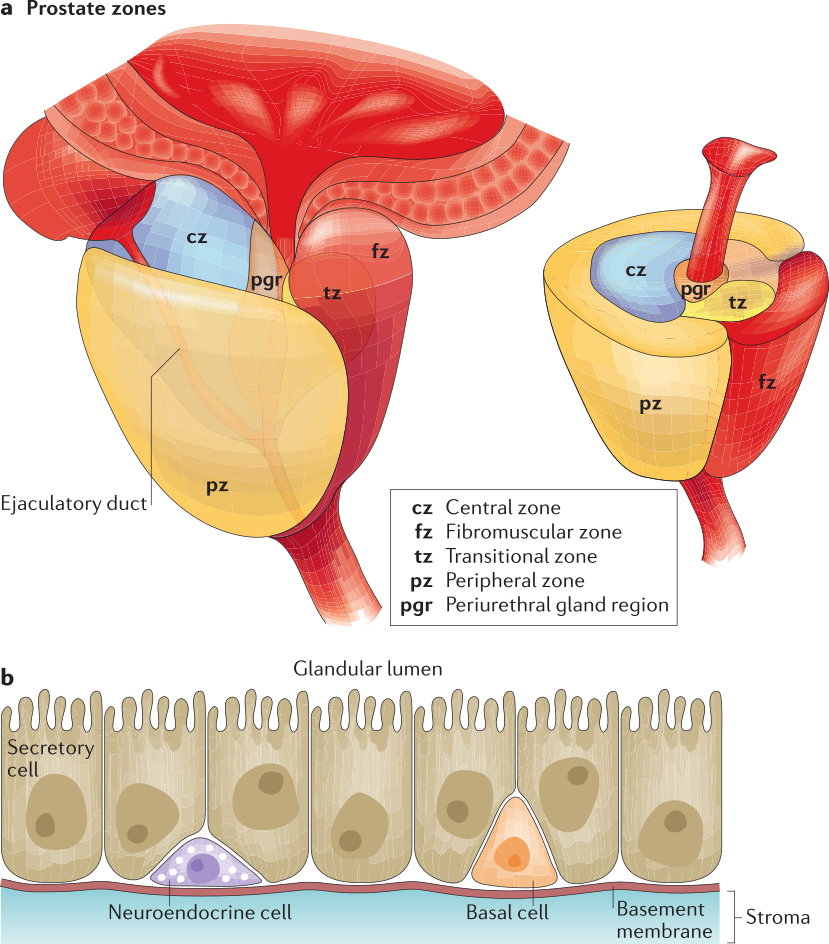
\includegraphics[keepaspectratio,width=\textwidth]{Introduction/Figures/prostateanatomy.png}
        \caption[Anatomy of the prostate gland]{\textbf{Anatomy of the prostate gland}. (\textbf{a}) General anatomical structure of the prostate. (\textbf{b}) Microscopic structure of the prostate. Permission granted for reuse from Springer Nature under license number 5982481051990 \cite{Verze2016Jul}}
        \label{prostateanatomy}
    \end{center}
\end{figure}

\subsubsection{Androgens and AR in prostate development and homeostasis}
The growth of the prostate begins in the foetus and is complete at sexual maturity. The prostate develops from the urogenital sinus (UGS), an epithelial-mesenchymal structure located at the base of the developing bladder, which, at 10-12 weeks postconception, commences prostatic morphogenesis via circulating androgens produced by the fetal testis \cite{Hamilton1959}. In females, the absence of androgens dictates that the UGS forms the lower portion of the vagina and the urethra. Initial prostatic morphogenesis occurs via the growth of epithelial buds from the urogenital sinus epithelium (UGE) into surrounding urogenital sinus mesenchyme (UGM), forming precise patterns of epithelial cords establishing lobular subdivisions of the prostate (Figure \ref{prostatedevelopment}) \cite{Timms1994May}. The epithelium then reorganises into two distinct cell populations: basal epithelial cells located along the basement membrane and tall, luminal cells (Figure \ref{prostateanatomy}b). During this time, the prostatic stroma differentiates into smooth muscle layers surrounding the prostatic ducts \cite{Wang2001Oct}. Once fully formed, the prostate does not undergo exponential differentiation again until puberty, when it reaches its mature size, shifting from stromal AR expression to epithelial AR expression (Figure \ref{prostatedevelopment}). Despite sustained levels of circulating androgens post-puberty, AR signalling in both the epithelium and stroma transitions from growth to a steady-state phase \cite{Vickman2020Jul}. Androgens, namely testosterone, are primarily secreted from the testis and, upon uptake by prostatic cells, are converted to dihydrotestosterone (DHT) via 5$\alpha$-reductase. DHT binds to the AR with two- to five-fold higher affinity than testosterone, yielding 10-fold AR signalling \cite{Gao2005Sep}. Therefore, androgen availability, AR expression and 5$\alpha$-reductase activity are all crucial to normal prostate development. In sexually mature males, the AR remains critical for the maintenance of the prostate. It has been demonstrated that following involution of the prostate, supplementation of androgens restores the prostate to its original size \cite{Isaacs2008Jun}.\par
The AR gene is located on the X chromosome and, like other members of the nuclear receptor family, the AR consists of three functional domains: the N-terminal domain (NTD), the DNA-binding domain (DBD) and the C-terminal ligand-binding domain (LBD), connected to the DBD via a hinge region \cite{Mangelsdorf1995Dec}. The highly conserved DBD links the AR to the promoter and enhancer regions of AR-mediated genes by direct DNA binding, allowing the NTD and LBD to activate transcription of AR genes, maintaining canonical differentiation. Defects in the AR gene can lead to dysregulation in the ratio between proliferation and cell death, of which androgen and AR are master regulators \cite{Denmeade1996Apr}. Defects of the AR gene can be caused by 1) point mutations causing substitutions or premature stop codons, 2) insertions and deletions (INDELs) causing frameshift mutations, 3) complete or partial gene deletion and 4) intronic mutations in splice sites affecting AR RNA splicing \cite{McPhaul2002Dec}. Progression towards prostate cancer (PCa) can be attributed to several AR-linked growth-promoting pathways. In $\sim$50\% of PCa tumours, gene fusions between \textit{TMPRSS2} and ETS family of transcription factors (ETS Transcription Factor ERG (\textit{ERG}) and ETS variant transcription factor 1) confer androgen responsiveness to members of the ETS family, resulting in cell-cycle progression \cite{Rubin2011Aug}. Three well-known cancer pathways (PI3K, Ras-Raf-MEK-ERK, RB) were shown to be dysregulated in primary PCa, however, analysis of AR pathway-associated genes revealed greater alterations when compared to other pathways, suggesting AR is indeed the master-regulator of PCa \cite{Taylor2010Jul}. The reliance of PCa on AR pathway perturbations is the rationale for the use of androgen deprivation therapy to treat PCa, as discussed in the following sections. 

\begin{figure}
    \begin{center}
        %\includegraphics[angle=90,origin=c,width=\textwidth, height=0.7\textheight,keepaspectratio]{Figure1.png}
        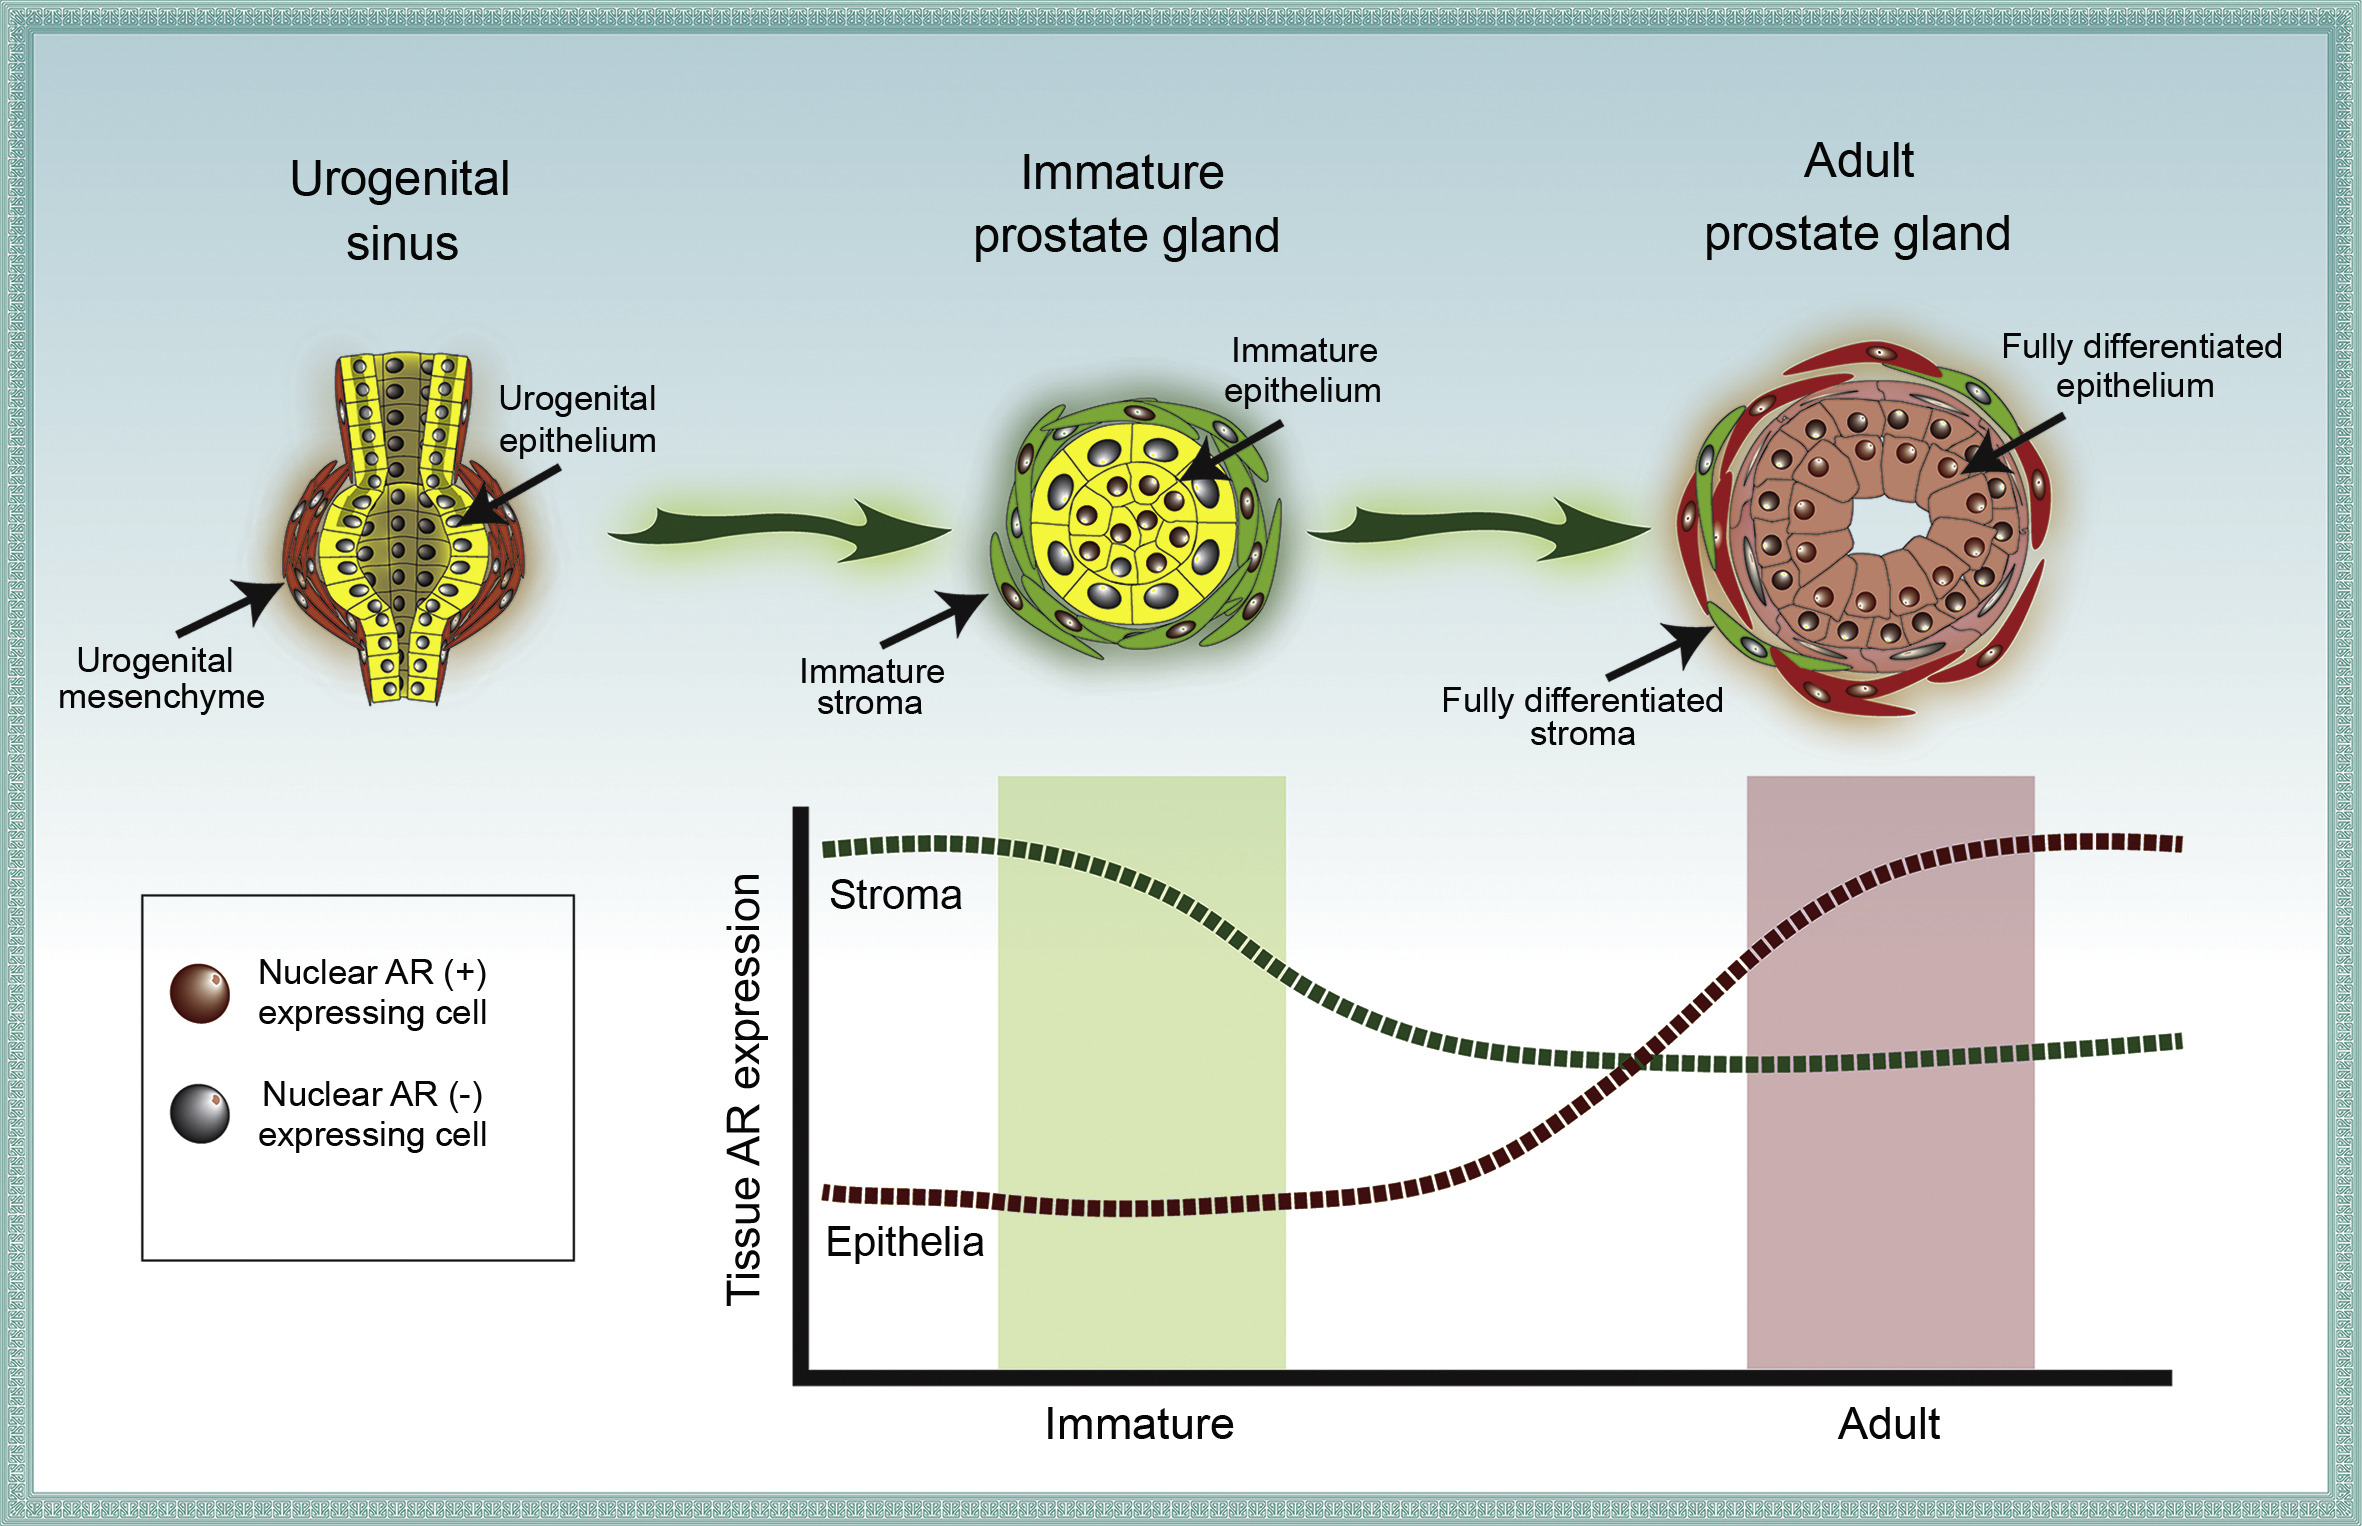
\includegraphics[keepaspectratio,width=\textwidth]{Introduction/Figures/prostatedevelopment.jpg}
        \caption[Development of the prostate]{\textbf{Development of the prostate} initiated by the development of the urogenital sinus (UGS), followed by extensions of prostatic buds to form an immature prostate gland. The adult prostate contains differentiated epithelial and stromal compartments. AR expression transitions from primarily stromal to epithelial during adult development. Figure reused under creative commons license \cite{Vickman2020Jul}}
        \label{prostatedevelopment}
    \end{center}
\end{figure}


\subsection{Prostate Cancer}
\subsubsection{Epidemiology}
PCa is the second most common cancer in men worldwide, accounting for 1 in every 14 cancer diagnoses and 15\% of all male cancers \cite{James2024Apr}, ranking second only to lung cancer in mortality rates \cite{BrayF}. Global incidence varies substantially (Figure \ref{prostatestatistics}), partly attributed to socioeconomic healthcare factors and the extent to which prostate-specific antigen (PSA) testing is used \cite{Culp2020Jan}. Consequently, the highest incidence rates occur in developed regions: Northern and Western Europe, Australia, New Zealand, North America, and Southern Africa (age-standardised rate of 35.5 per 100,000), whilst under-developed countries in regions such as sub-Saharan Africa, parts of South America and Eastern Europe rank the lowest in incidence rates (12.6 per 100,000) \cite{Nyame2020Jan}. Mortality outcomes are strongly influenced by the availability of screening and treatment; thus, regions with lower reported incidence frequently exhibit higher mortality rates, reflecting disparities in healthcare access rather than differences in underlying disease burden \cite{Nyame2020Jan}. Of note, elevated incidence of PCa in Caribbean and sub-Saharan African countries may be linked to genetic variants associated with PCa occurring more frequently in men with West African ancestry \cite{Culp2020Jan, Rebbeck2013Feb}. This is evident in North America, where African American men are twice as likely to contract the disease \cite{Brawley2012Sep}. In Asian countries, incidence and mortality rates are low (Figure \ref{prostatestatistics}); however, when Asian men migrate to the United States, their risk increases \cite{Kimura2012Sep}, indicating that low incidence and mortality rates in Asia are potentially due to a lack of population-based data across most of the countries in this region \cite{Baade2013Jun}.  In Ireland, approximately 4000 men are diagnosed with PCa annually, with 1 in 6 expected to contract the disease in their lifetime \cite{NCRI}. The overall five-year survival rates for Irish men diagnosed with PCa are 92.5\% for primary localised PCa \cite{NCRI}, reflecting advancements in effective treatment and earlier detection through increased testing of Irish men.

\begin{figure}
    \begin{center}
        %\includegraphics[angle=90,origin=c,width=\textwidth, height=0.7\textheight,keepaspectratio]{Figure1.png}
        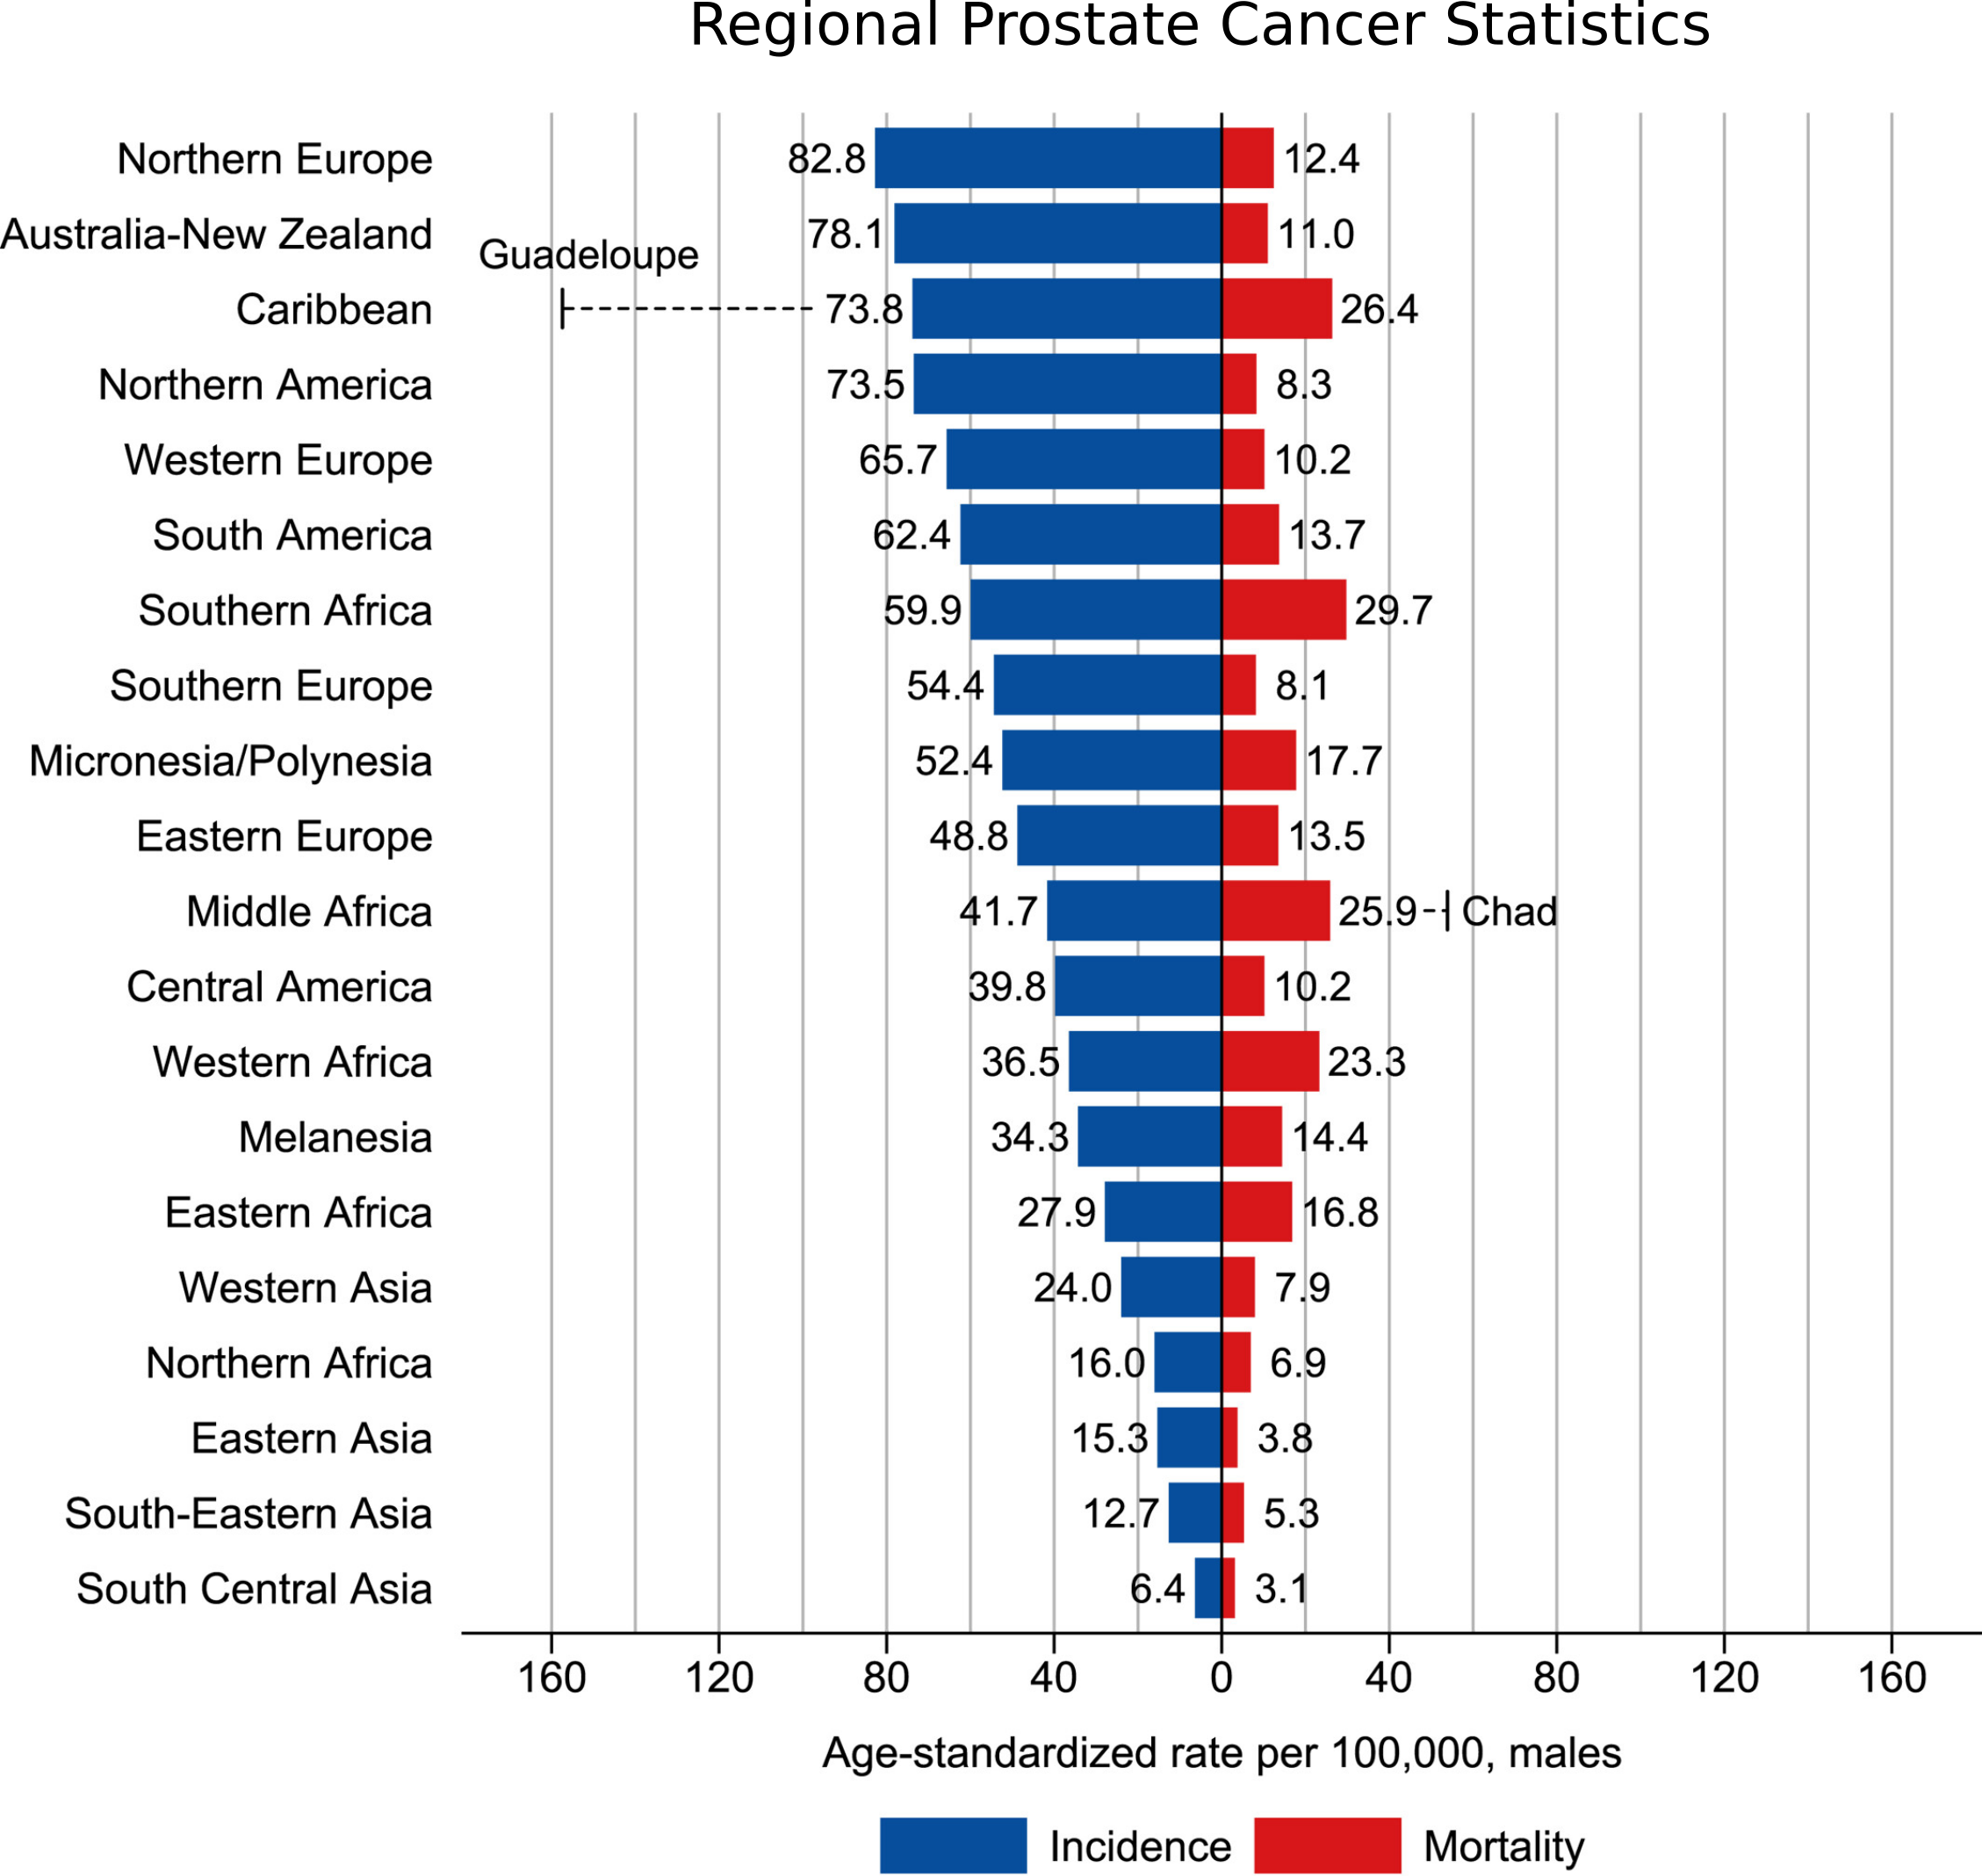
\includegraphics[keepaspectratio,width=\textwidth]{Introduction/Figures/prostatestatistics.png}
        \caption[Region-specific bar chart of prostate cancer incidence]{\textbf{Region-specific bar chart of prostate cancer incidence} and mortality age-standardised rates (GLOBCAN 2022). Permission granted for reuse from John Wiley and Sons under license number 5982410882196 \cite{Bray2024May}}
        \label{prostatestatistics}
    \end{center}
\end{figure}

\subsubsection{Aetiology}
Established risk factors for PCa include age, ethnicity, obesity and family history. Age-specific incidence rates and the aggressiveness of PCa rise after age 55 and peak at ages 70-74 \cite{Gann2002, Milonas2019Sep}. The population-based Surveillance, Epidemiology, and End Results (SEER) study reveals the 10-year risk of PCa increases from 2.3\% at age 50 to 7.3\% at 70. In addition, $\sim$60\% of men diagnosed with PCa are older than 65 \cite{SEER}. Epidemiological studies show African Americans are approximately 60\% more likely to develop PCa and exhibit nearly double the mortality rate when compared to white American males \cite{Gann2002}. It is unclear whether this stems from differences in socioeconomic status variables and access to healthcare or if there exists an inherent difference in the underlying PCa biology of both cohorts \cite{Tewari2005Dec}. As previously mentioned, men of West African descent harbour more genetic variants linked to PCa \cite{Culp2020Jan, Rebbeck2013Feb}; however, it is more likely that an interaction between genetic and environmental factors is responsible for increased PCa risk in African Americans. \par
The terms familial and hereditary PCa imply increased risk but are not analogous. Familial PCa is a result of cancer clustering within a family, often due to shared environmental factors, whilst hereditary PCa is genetic and is defined as a family with 1) three generations affected, 2) three first-degree relatives affected or 3) two relatives affected before age 55 \cite{Potter2000}. The pooled incidence rate ratio for men with an affected brother or father is 2.48 (95\% CI 2.25-2.74), with an affected brother yielding a higher rate ratio of 3.14 (2.37-4.15) than an affected father alone (2.35; 2.02-2.72), and the pooled estimate for two or more affected first-degree members is 4.39 (2.61-7.39). Strikingly, first-degree family history increases the incidence rate in men under 65 (RR:2.87, CI:2.21-3.74) compared to men over 65 with no familial history (1.92, 1.49-2.47) \cite{Kicinski2011Oct}. \par
Studies have revealed a positive correlation between high BMI and high-grade nonmetastatic and metastatic PCa \cite{Rodriguez2007Jan}. Furthermore, patients with a BMI $>$30 are at risk of developing metabolic syndrome (MetS), a cluster of cardiovascular risk factors including hypertriglyceridemia, central adiposity, hypertension, low HDL-C, and insulin resistance \cite{Grundy2004Jan}. MetS has been shown to harbour a positive association with pathologic Gleason score $>$8 and biochemical recurrence (BCR) of the disease \cite{Gacci2017Jun}. BCR is defined as PSA levels of $>$0.2ng/mL confirmed by a secondary measurement following undetectable PSA levels post-surgery \cite{Amling2001Apr}. However, levels exceeding $>$0.4ng/mL appear to more accurately predict the development of distant metastases \cite{Toussi2016Jun}.  

\subsubsection{Disease initiation}
PCa often exhibits high levels of interpatient heterogeneity (ethnic/geographical) and intrapatient heterogeneity. Cells within different tumour foci may arise from cellular ancestors that transformed independently or from a single transformed ancestor clone generating distinct clones and subclonal lineages \cite{Rebello2021Feb, Boyd2012Nov}. Consequently, the true cell of origin for all prostatic adenocarcinomas remains a contentious issue. PCa cells are thought to originate from basal or luminal prostatic epithelial cells, however, non-epithelial cells can also play a role in PCa initiation and progression \cite{Goldstein2010Jul, Chua2014Sep, Lee2015Dec}. Approximately 25\% of men in their 50s and up to 90\% in their 80s may present with abnormal, non-cancerous cell growth and proliferation of luminal epithelial cells in the transition zone, known as benign prostatic hyperplasia (BPH) \cite{Bushman2009Nov}; however, BPH is not considered to be a precursor for PCa cells, which by definition, must possess the capacity to invade the basement membrane to be classified as cancerous \cite{Kristal2010May}. \par 
In contrast to BHP, non-malignant lesions termed high-grade prostatic intraepithelial neoplasia (PIN) are frequently detected adjacent to PCa cells and are considered precursors to PCa \cite{Rebello2021Feb}. PIN occurs in the peripheral regions of the prostate gland and is characterised by intraglandular proliferation of luminal epithelial cells accompanied by compromised integrity of the basal cell layer \cite{Ayala2007Aug, Bostwick2004}. Morphologically, high-grade PIN cells display enlarged nuclei with prominent cytoplasmic basophilia and nucleoli \cite{Bostwick2004Mar}. A series of genomic alterations common to both high-grade PIN and PCa cells may serve as clues to PCa initiation: silencing of GSTP1 enzyme resulting in increased oxidative cell damage \cite{Lee1994Nov}, inactivation of tumour suppressor genes due to loss of heterozygosity on 8p12-21 detected in 63\% of PINs and 90.6\% of PCa cells \cite{Emmert-Buck1995Jul}, loss of \textit{NKX3-1} expression correlating to tumour progression \cite{Asatiani2005Feb} and amplification of \textit{ARNT} \cite{Kim2013Feb}. Jung et al. demonstrated that PCa genomes are direct descendants of high-grade PIN genomes \cite{Jung2016May}, postulating that high-grade PIN genomes require additional genomic modifications, such as \textit{TMPRSS2-ERG} fusions, to progress to PCa \cite{Fraser2017}. \par

\subsubsection{Screening and early detection}
Screening for PCa is the primary method for detecting localised PCa in asymptomatic men at a stage when the disease is potentially curable. Ideally, screening should be able to discriminate between tumours that require immediate action and definitive therapies with intent to cure from tumours that remain indolent and can be managed through active surveillance. The two main screening strategies for PCa are 1) a digital rectal exam (DRE) and 2) a PSA test. The former involves physical palpation of the prostate gland to assess its texture, checking for hard sections or nodules that may be cancerous, whilst the latter is a minimally invasive blood test assessing PSA levels. In men younger than 60, a PSA level of $<$2.5ng/mL is considered normal, while in men over 60, PSA levels $<$4.0ng/mL are considered non-elevated. Increased PSA levels occur naturally with age, however, increased PSA levels are also a marker of PCa due to malignant PCa cells lacking a structurally intact basal layer that otherwise restricts the extravasion of PSA to the prostatic ducts and bloodstream \cite{David2024Sep}. Thus, PSA screening has received negative attention in the literature, as elevated levels of PSA may be due to normal prostate cells or noncancerous conditions such as BPH or prostatitis, resulting in substantial risk of overdiagnosis and overtreatment of clinically indolent PCa \cite{JuliaHayes2014Mar, Ilic2013Jan}. A meta-analysis of published studies relating to the benefits of PSA screening substantiates this point: 570 men were needed for screening to prevent one death from PCa \cite{Tesfai2024May}. Despite this, the European Randomised Study of Screening for Prostate Cancer study (n=182,160) revealed a 20\% reduction in PCa-specific mortality over a follow-up of 16 years, demonstrating the ability of PSA screening to reduce PCa mortality at a population level \cite{Hugosson2019Jul}. \par
In the event of a high PSA reading, clinicians may pursue other avenues to determine if biopsy is necessary. Free PSA tests determine the ratio of PSA bound to antichymotrypsin (ACT) vs. the level of unbound PSA in a blood sample. Christensson et al. reported that PCa patients exhibit higher proportions of PSA-ACT than those with BPH \cite{Christensson1993Jul}, thus a result showing lower percentages of free PSA compared to PSA-ACT may warrant a biopsy. In patients presenting with high PSA levels and a negative biopsy, a molecular test to assess levels of mRNA from the prostate cancer antigen 3 (\textit{PCA3}) gene can be used to adjudicate if a repeat biopsy is required. Regardless of the chosen screening strategy, current guidelines recommend a multivariate approach accounting for factors such as age and family history to make an informed decision-making process for each patient \cite{Mottet2017Apr}.

\subsubsection{Diagnosis}
Pathways for PCa diagnosis when a DRE examination or PSA test results raise suspicion of PCa include sampling the prostate via transrectal ultrasound (TRUS) biopsy. TRUS-guided biopsies systematically sample 10-12 cores for histopathological evaluation, with a 30-40\% chance of detecting PCa in its first pass \cite{Ploussard2014Jan}. Drawbacks of TRUS biopsies include the risk of developing potentially life-threatening Gram-negative sepsis, estimated to be 3\% \cite{Loeb2013Dec}, bleeding, erectile dysfunction, and incomplete sampling of the prostate. By design, samples are taken from the peripheral zone bilaterally from the apex to the base of the gland, omitting parts of the anterior and caudal prostate. This strategy is of concern as the anterior apex has been found to frequently harbour cancerous cells, which when missed, require additional biopsies \cite{Moussa2010May}. More recently, the 3-Tesla multiparametric MRI (mpMRI) and an MRI-targeted transperineal biopsy have superseded the TRUS biopsy. mpMRI considers multiple parameters: 1) T1 and T2 anatomical imaging; 2) diffusion-weighted imaging (assessing the movement of water, known to be restricted in areas of cancer); and 3) contrast-enhanced imaging whereby the enhanced blood supply to cancerous cells takes up and releases the dye more quickly \cite{Moore2013Jan}. MRI results are assessed according to the Prostate Imaging Reporting and Data System (PI-RADS) on the scale of 1-5, with scores greater than or equal to 3 indicative of clinically significant prostate cancer, and a decision regarding biopsy is made \cite{Klotz2021Apr}. Transperineal biopsies carry a lower risk of infection (0.2\%) than transrectal biopsies, as the needle route bypasses the rectal wall, avoiding potential contamination. Nonetheless, the European Association of Urology (EAU) guidelines recommend combining targeted and systematic biopsies regardless of approach \cite{Chernysheva2026Sep}.

    \par
When establishing a diagnosis, each biopsy site is reported individually, including information on location, differentiation grade and extent. Differentiation grading may follow the Gleason scoring system or the International Society of Urological Pathology (ISUP) grading. The Gleason scoring system has been the standard for $>$40 years, in which microscopic evaluation of histological features within the tumour architecture is used to classify the tumour as poorly-differentiated (high grade) or well-differentiated (lower grade) \cite{Gleason1974Jan, Kweldam2019Jan}. The final Gleason score is the summation of the first and second most prominent Gleason pattern grades, with low ($<$6), intermediate (7) or high (8-10) comprising the final Gleason scores. In 2014, the Gleason scores were reorganised into ISUP grades 1-5, primarily to account for the differentiation of Gleason score 7, which may be composed of 3+4 or 4+3 observations (the predominant pattern is recorded first), in addition to the amalgamation of Gleason scores 9 and 10 to ISUP grade 5 \cite{Epstein2015Jul}. The World Health Organisation adopted the ISUP grading system in conjunction with PSA results and clinical T category (cT) to refine patient diagnoses further: patients are classified as low risk (cT1-cT2a, PCa $<$10ng/mL, ISUP grade 1), intermediate risk (cT2b or PSA $>$10-20ng/mL or ISUP grade 2) and high risk ($>$cT2b or PSA $>$20ng/mL or ISUP grade $>$3) \cite{Mottet2017Apr}.

\subsubsection{Disease progression}
PCa progresses in most patients, characterised by rising PSA levels suggestive of elevated AR activity owing to the proliferation of luminal epithelial cells. Early-stage PCa is androgen-dependent; therefore, traditional treatment strategies focus on attenuating the AR signalling pathway by blocking androgen binding to the AR, or via inhibition of transcriptional activity of the AR using androgen-deprivation therapy (ADT) or second-generation antiandrogens \cite{Li2025Feb}. These methods have been shown to greatly enhance progression-free survival rates of patients \cite{Fizazi2017Jul}, yet tumours may still arise from a subpopulation of cells that are resistant de novo or acquire resistance induced by AR antagonists, leading to a castrate-resistant prostate cancer (CRPC) phenotype. These resistant PCa cells re-activate AR signalling through a variety of mechanisms: AR gene amplification, AR mutations (Table \ref{ARmuts}), and AR splice variants such as \textit{AR-V7} \cite{Csizmarik2021Oct}. \par

\subsubsection{Management and Treatment}
Patients diagnosed with localised PCa have 3 options: expectant management, surgery and radiation. Expectant management does not involve a definitive treatment following diagnosis and is typically reserved for low-risk PCa. It can be classified as watchful waiting where symptoms are treated with palliative intent, or active surveillance involving PSA testing, DRE or biopsies with intent to cure patients who develop significant PCa disease \cite{Filson2015Jul}. Age is the primary factor guiding the choice of expectant management strategy, with the final decision typically being patient-led. Active surveillance is the preferred choice for younger men with low-risk PCa (Gleason $\leq$7) \cite{Chen2016Jun}. In the Prostate Testing for Cancer and Treatment (ProtecT) trial, 1643 men with localised PCa were randomised into active monitoring (n=545), surgery (n=553) or radiation (n=545). Whilst the number of men who experienced clinical progression of PCa (112 vs. 46 vs. 46) or experienced metastasis (33 vs. 13 vs. 16) at 120 months was roughly double for men in the active surveillance arm of the study, these results had no statistically significant bearing on overall mortality. Only 8 (1.5\%), 5 (0.9\%) and 4 (0.7\%) of men treated using active surveillance, surgery and radiation, respectively, died from PCa \cite{Hamdy2016Oct, Donovan2016Oct}. \par
For men presenting with Gleason score $>$7 and PSA 10-20ng/mL, surgery and radiation are the primary methods for treatment. The ProtecT trial showed no significant difference between surgery vs. radiation with respect to clinical progression, metastasis and overall survival. Yet, surgical and radiation treatments reduced the risk of clinical progression and metastasis when compared to active surveillance \cite{Hamdy2016Oct, Donovan2016Oct}. Whilst longer-range follow-up data is unavailable in this study, it stands to reason that fewer BCR and metastasis events could lead to improved long-term overall survival at the population level. Furthermore, for men treated with surgery, adjuvant radiation has been shown to reduce the occurrence of BCR in patients with pT3 tumours (HR=0.51, 95\% CI=0.37-0.70, P=$<$0.0001) compared to `wait-and-see' following surgery \cite{Wiegel2014Aug}. \par
Androgen deprivation therapy (ADT) agents remain the mainstay treatment for men with metastatic castrate resistant prostate cancer (mCRPC). ADT agents can act as luteinizing hormone-releasing hormone agonists/antagonists, reducing testosterone production by the testes, or as antiandrogens, preventing testosterone from binding to the AR. Alternatively, they can act as androgen synthesis inhibitors, blocking CYP17. The first ADT agent that showed prolonged survival among men with mCRPC was docetaxel \cite{Sartor2018Feb}. Two phase 3 trials demonstrated significant overall survival benefits of docetaxel vs. control HR=0.76, 95\% CI=0.62-0.94, P=0.009 and HR=0.8, 95\% CI=0.67-0.97, P=0.02 \cite{Petrylak2004Oct, Tannock2004Oct} however, patients assigned to docetaxel experienced fever, cardiovascular events, nausea and vomiting, metabolic disturbances and neurologic events at a higher rate than the control group \cite{Petrylak2004Oct}. Two new second-generation ADT agents, abiraterone and enzalutamide, differ in their actions in the androgen axis: abiraterone acetate inhibits androgen biosynthesis, whilst enzalutamide inhibits AR signalling by binding the AR receptor \cite{Litwin2017Jun}. Both have been shown to slow disease progression and improve overall survival, whether before or after treatment using the first-generation agent docetaxel \cite{deBono2011May, Ryan2013Jan, Scher2012Sep, Beer2014Jul}. \par
Advances in the integration of genomic testing into the diagnostic pathway may facilitate a tailored approach to an individual's specific tumour molecular biology; detecting aberrations in DNA repair genes of the AR can be used to rule out patients who are unlikely to respond to docetaxel, abiraterone or enzalutamide \cite{Mateo2015Oct}. Similarly, detection of the AR-V7 splice variant, which lacks the ligand-binding domain targeted by abiraterone and enzalutamide, has been associated with primary resistance to these agents \cite{Antonarakis2014Sep}. Incorporating these genomic markers into treatment selection may therefore help clinicians avoid ineffective therapies, sparing patients unnecessary toxicity and enabling more rapid transition to a treatment strategy likely to provide clinical benefit.


\paragraph{AR Amplification}
\noindent Clinically, AR amplification is significantly overrepresented in CRPC tumour samples that are refractory to ADT when compared to benign tissue or primary PCa tissue (Figure \ref{armutations}) \cite{Bubendorf1999Feb}, suggesting that CRPC cells undergo selective pressure to circumvent ADT intervention. Mechanistically, AR amplification increases AR expression, resulting in hypersensitivity to low levels of circulating androgens \cite{Waltering2009Oct}. A recent study has detailed a novel interaction between the overexpression of transcription factors MYB and AR, whereby MYB overexpression facilitates ligand-independent nuclear localisation of transcriptionally active AR, sustaining AR transcriptional activity under ADT conditions \cite{Srivastava2012Mar, Srivastava2021Nov}. Notably, AR amplification is more common in patients exhibiting biochemical recurrence after treatment using enzalutamide compared to abiraterone (58\% vs. 17\% P=0.02) \cite{Azad2015May}. Patients with AR gain in cell-free DNA have poorer progression-free survival (HR: 5.52, 95\% CI: 2.57-11.83, P $<$0.0001) and overall survival rates (HR: 12.06, 95\% CI: 4.94-29.49, P $<$0.0001) compared to normal AR status patients when treated with enzalutamide or abiraterone \cite{DelRe2021Jun}. AR amplification may be a useful biomarker for identifying candidates suited to treatment using second-generation ADT. \par

\paragraph{AR Mutations}
\noindent Similar to AR amplification, AR mutations confer a selective advantage for tumor cells in a low androgen environment resulting from hormone therapy. The first AR mutation identified was a missense mutation T877A, located in helix 11 of the AR LBD, which when mutated, showed robust AR transcriptional activity and could not be inhibited by the nonsteroidal antiandrogen bicalutamide \cite{Sun2006Jun}. The replacement of T877 by alanine facilitates promiscuous activity, where the mutant AR can bind to other hormones and analogs such as progestins, estrogens and cortisol. The binding of progesterone, estradiol or flutamide has been shown to activate AR-T877A \cite{Sack2001Apr}. Also located in the LBD, the mutation H874Y increases the size of the ligand-binding pocket, accommodating nonandrogenic steroid ligand activation by nilutamide \cite{Duff2005Dec}. Joseph et al. and Korpal et al. both report antagonist-to-agonist switching of the AR due to the point mutation to the LBD at F876L following patient treatment using enzalutamide \cite{Joseph2013Sep, Korpal2013Sep}. Overall, there is clear evidence that disease progression following ADT therapy can be facilitated by treatment-specific induced mutations to the AR, broadening the ligand specificity of the AR giving rise to a `mutator phenotype' \cite{Steinkamp2009Apr, Bielas2006Nov}. \par

\paragraph{AR Splice Variants}
\noindent Dehm et al. and Hu et al. identified AR splice variants producing a truncated AR protein which remains constitutively active in the absence of androgens \cite{Dehm2008Jul, Hu2009Jan}. AR splice variants are generated from transcribed intronic regions of intron 3, termed `cryptic exons' (CE1, CE2 and CE3) which, due to somatic nonsense mutations, splice a combination of cryptic exons to exon 3 of the AR, generating AR-V1 to AR-V7 splice variants \cite{Hu2009Jan}. Each of these AR variants produce premature termination codons downstream of the AR DBD, resulting in truncated ARs missing a LBD capable of evading nonsense-mediated decay \cite{Ajiboye2017Jun}. Regarding disease progression, elevated expression of AR-V7 is observed in CRW22 patient-derived xenographs refractory to abiraterone and enzalutamide \cite{Li2013Jan, Zhu2020Nov}. \par

Irrespective of the underlying genomic abberations, most patients will acquire resistance to ADT, progressing to CRPC and ultimately metastatic CRPC, which carries a far worse prognosis. Therefore, it is of utmost importance to investigate biomarkers associated with disease progression to effectively stratify patients, identify novel targets and develop personalised treatment strategies for patients. 

\begin{figure}
    \begin{center}
        %\includegraphics[angle=90,origin=c,width=\textwidth, height=0.7\textheight,keepaspectratio]{Figure1.png}
        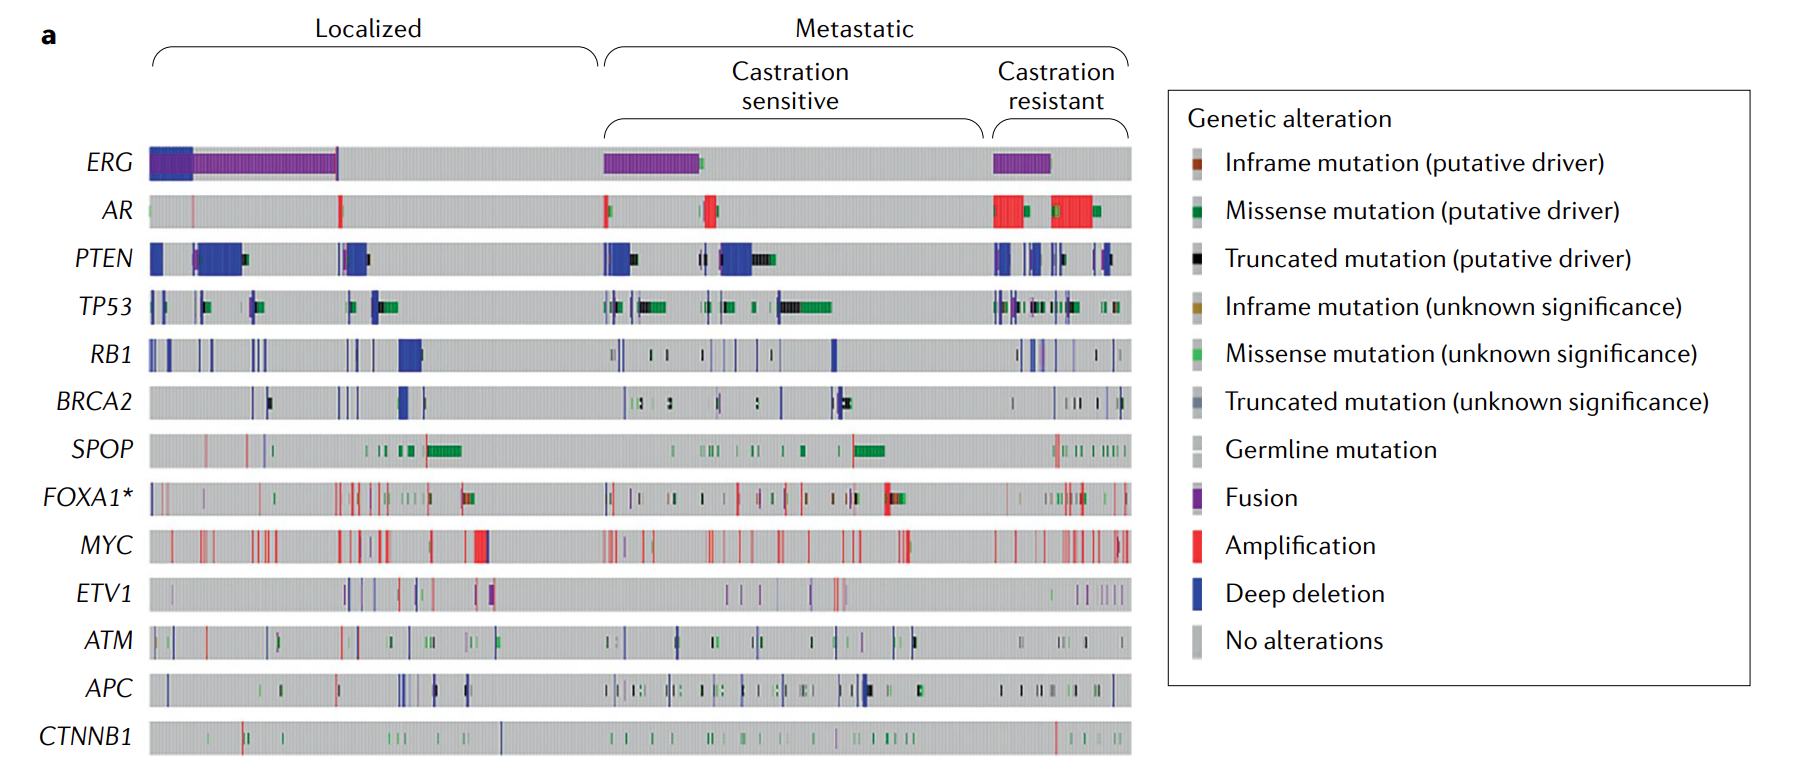
\includegraphics[keepaspectratio,width=\textwidth]{Introduction/Figures/AR_mutations.png}
        \caption[Genetic alterations in prostate cancers]{\textbf{Genetic alterations in prostate cancers}: localized, metastatic castration-sensitive prostate cancer (mCSPC) and metastatic castration-resistant prostate cancer (mCRPC) (localized, 494 samples; mCSPC, 424 samples; mCRPC, 150 samples). Permission granted for reuse from Nature Reviews Disease Primers under license number 5996481096401 \cite{Rebello2021Feb} }
        \label{armutations}
    \end{center}
\end{figure}

\iffalse
Cancer-associated fibroblasts (CAFs) are abundantly present in the prostate tumour microenvironment (TME), with reduced AR expression in CAFs considered a prognostic factor of PCa progression, suggesting CAFs may act as a negative regulator of PCa development \cite{Tang2021Oct}. Palethorpe et al. demonstrated \textit{in vitro} AR activation in human prostate myofibroblasts retarded growth of multiple PCa cell lines (PC3, Du145, C4-2B, LNCaP) \cite{Palethorpe2018Apr} whilst Cioni et al. showed loss of AR in CAFs downregulated \textit{CCL2} and \textit{CXCL8} cytokine expression, facilitating PCa cell migration \cite{Cioni2018Aug}. Second-generation therapies such as enzalutamide inhibit AR-mediated PCa growth, but consequently elevate metastasis-related markers N-cadherin \cite{Jennbacken2010Jun}, Cadherin-11 \cite{Lee2010May, Chu2008Aug} and nestin \cite{Kleeberger2007Oct}. In a phase II study, abiraterone was shown to successfully reduce PSA levels by 50\% or more in 79\% of patients, yet 43.5\% of patients experienced bone scan flare lesions indicative of bone metastases \cite{Ryan2011Jun}. 
\fi

\renewcommand{\arraystretch}{1.4}
\begin{table*}[h!]
\caption[Summary of selected androgen receptor mutations]{\textbf{Summary of selected androgen receptor mutations}. LBD: Ligand-binding domain; Nterm: amino-terminal domain. Full mutation catalogue available at \href{https://androgendb.mcgill.ca/}{https://androgendb.mcgill.ca/} \cite{Gottlieb2012May}.\label{ARmuts}}
\resizebox{\textwidth}{!}{%
\begin{tabular}{llcp{9cm}r}
\toprule
\textbf{Mutation} & \textbf{Position} & \textbf{Exon} & \textbf{Description} & \textbf{Reference} \\
\midrule
Substitution & L701H   & 4/LBD  & Reported in hormone-refractory PCa patients. Highly responsive to AR activation via circulating ligands, cortisol and cortisone. & \cite{vandeWijngaart2009Dec} \\
Substitution & T877A   & 8/LBD  & Exhibits robust AR activity in the presence of antiandrogens. & \cite{Sun2006Jun, Chen2004Jan} \\
Substitution & W741C   & 5/LBD  & Bicalutamide-liganded W741C mutant AR coactivated by $\beta$-catenin. & \cite{Masiello2004Oct} \\
Deletion     & CAG-repeats & 1/Nterm & Shorter repeats correlate with younger diagnosis, higher grade and higher stage PCa. & \cite{Bratt1999Oct} \\
Substitution & F876L   & 8/LBD  & Abolishes antagonistic activity of enzalutamide. & \cite{Joseph2013Sep, Korpal2013Sep} \\
\bottomrule
\end{tabular}%
}
\end{table*}

\subsection{Biomarkers in prostate cancer}
Detection of early stage PCa relies on PSA testing and a DRE, whilst localised advanced PCa can benefit from biopsy tests to establish cancer stage. In an effort to address the transitional stages of PCa progression, several biomarker tests have been developed to date. The prostate health index (PHI) attempts to increase the diagnostic value of PSA by combining total PSA, \% free PSA and [-2]pro-PSA to produce a scoring system \cite{Le2010Apr}. Intended as a diagnostic tool, its recommended use is for patients presenting with PSA levels between 2.0ng/mL and 10ng/mL. The PHI score outperformed each of its constituent parts (0.74 AUC (PHI), 0.72 \%[-2]proPSA, 0.63 [-2]proPSA, 0.61, \%free PSA and 0.56 total PSA) \cite{Stephan2013Jan}. For the diagnosis of advanced PCA, the 4K score was developed combining four different kallikrein markers (total PSA, \%free PSA, intact PSA, human-kallikrien-2 (hK2)), patient age and DRE results \cite{Vickers2010May}. Nordstrom et al. combined the 4K and PHI scoring systems in a study on 513 men with PSA levels ranging from 3.0 - 13.0ng/mL \cite{Nordstrom2015Jul}. Whilst AUC results from the 4K and PHI test were indistinguishable in detecting PCa of any form and advanced PCa, the authors used cut-off values (10\% 4K score, 39 PHI score) to stratify patients effectively. Results of the study demonstrated 29\% of unnecessary biopsies could be spared, however, 10\% of high-grade PCa cases would be missed using the cut-off points. \par
\subsubsection{Messenger RNAs
}
In 2015, the first genetic diagnostic test was developed termed SelectMDx, comprising a two gene panel (\textit{DLX1} and \textit{HOXC6}) PSA, age, history of prostate biopsy and family history \cite{Leyten2015Jul}. It has been shown that the use of SelectMDx in patients with PSA levels $>$3 ng/mL can reduce overdiagnosis and overtreatment and ultimately reduce total costs per patient and increase health-related quality of life \cite{Dijkstra2017Nov}. A secondary panel developed by MDx Health termed ConfirmMDx focuses on epigenetic changes in \textit{GSTP1}, \textit{APC} and \textit{RASSF1} genes in an effort to detect the `halo effect' surrounding tumor foci with abberations to any gene constituting a positive result \cite{Partin2014Apr}. As ConfirmMDx is predecated on detecting cancer, it cannot be used as a tool to rule out clinically significant PCa \cite{Leapman2016Feb}. As such, its recommendation is towards men before repeat biopsy following an initial negative biopsy \cite{Kretschmer2017Dec}. \par
Concerning prognostic tests for PCa, the Oncotype DX Genomic Prostate Score (GPS) assay evaluates 12 cancer-related genes and 5 reference genes to produce a score between 0-100, with 40 being the cut-off point for high-risk disease \cite{Klein2014Sep, Cullen2020Sep}. The Prolaris test, based on work by Cuzick et al. \cite{Cuzick2011Mar} evaluates 31 genes involved in cell cycle progression (CCP) creating a risk score effectively stratifying patients into $\leq$0, $>$0 to $\leq$1, 1 to $\leq$2 and $>$2 CPP score. An increase by one unit of the CCP score was able to independently predict BCR (HR=1.77, 95\% CI=1.40–2.22, P=$<$0.0001). The CCP was also able to significantly predict overall survival (HR=2.57, 95\% CI=1.93–3.43, P=$<$0.0001) \cite{Cuzick2011Mar}. The ProMark test utilises 12 proteomic biomarkers as a prognostic tool to detect aggressive PCa and lethal PCa \cite{Shipitsin2014a, Shipitsin2014b}. In a clinical validation study, the panel was refined to 8 proteomic signatures and using a cut-off score of $\leq$0.33, the authors found positive results in distinguishing low favourable vs. favourable pathology results (AUC 87.2\%) \cite{Blume-Jensen2015Jun}. Finally, the Decipher 22-gene panel based on genes involved in cell proliferation, androgen signalling, immune system modulation, cell cycle progression and cell structure, is primarily used to predict systemic progression of PCa following definitive therapy. The scoring system falls between 0-1, with values $>$0.6 considered high risk for progression \cite{Nakagawa2008May}. In an external evaluation study, Decipher was used to stratify patients into low risk $>$0.4, intermediate risk 0.4-$>$0.6 and high risk $>$0.6, effectively predicting freedom from BCR (0.78 AUC) and metastasis (0.80 AUC) in a cohort of 139 patients who recieved adjuvant or salvage radiotherapy following radical prostectomy \cite{Den2014Aug}. \par
A report from the International Society of Urological Pathology (ISUP) commented that genomic classifiers may provide utility in predicting disease progression under an active surveillance or postradical prostatectomy setting, if the tumor focus harboring the disease is adequately sampled. In addition, the report recommended further studies to assess the performance of the genomic signatures in relation to the heterogeneity inherent to needle biopsy samples, and to provide recommendations for sampling (which biopsy to use, multiple sampling from the same or different tumor foci) \cite{Lotan2020Jul}. Given that current PCa mRNA biomarkers are not a panacea, the research community must continue to search for new biomarkers that can aid in early diagnosis and prognosis of the patient as well as predict patient response to treatments. One such avenue is exploring non-coding RNAs involved in the competing endogenous RNA network, in which circular RNAs, microRNAs and messenger RNAs form a regulatory network capable of influencing gene expression in both normal and disease-based settings. 

\subsubsection{Micro RNAs}
Micro RNAs (miRNAs) are small 18-24 nucleotide non-coding RNAs that regulate the transcription of mRNAs by binding to complementary sequences in target mRNA, consequently blocking mRNA transcription or promoting degradation of the transcript \cite{Valencia-Sanchez2006Mar}. miRNAs can be found in several bodily fluids, including blood, urine, semen, and saliva, among others, exhibiting tissue-specific expression and dysregulation in cancer \cite{Weber2010Nov, Lin2015Jun}. Furthermore, miRNAs can be accurately quantified using techniques such as qRT-PCR, microarrays and small RNA sequencing, making them ideal candidates as biomarkers \cite{Fabris2016Aug}. \par
In PCa, miRNAs play important mechanistic roles, including inhibiting apoptosis, promoting cell proliferation, epithelial to mesenchymal transition (EMT) and growth under androgen-independent settings \cite{Bryant2012Feb} (Table \ref{PCamiRNAs}). Several studies have investigated the role of miRNAs as biomarkers in PCa, finding differentially expressed miRNAs according to PSA level, Gleason score and treatment using docetaxel \cite{Endzelins2017Nov, Mitchell2008Jul, Lin2014May}. Matin et al. demonstrated the diagnostic value of miR-4289, miR-326, miR-152-3p and miR-98-5p in differentiating PCa patients and healthy controls (AUC 0.88) \cite{Matin2018Apr}, whilst Sharova et al utilised miR-106a, miR-130b and miR-223 to distinguish localised PCa vs. BHP (AUC 0.84 vs. PSA only; AUC 0.56), aiding clinical decision making and avoiding unnecessary biopsies \cite{Sharova2016Jun}. \par
In addition to evaluating standalone miRNA signatures, researchers have begun constructing miRNA-mRNA bipartite networks composed of differentially expressed RNAs and predicted miRNA-mRNA pairs exhibiting inverse expression to model the regulatory effects of miRNAs \cite{Naghizadeh2023Jul, Lin2018Dec, Zhang2014Dec}. This `knowledge-based filtering' method has the potential to reveal miRNAs and mRNAs associated with cancers that may otherwise be omitted using traditional machine learning feature selection techniques. 


\begin{table*}[h!]
\centering
\caption[miRNAs upregulated in PCa]{\textbf{miRNAs upregulated in PCa}}
\resizebox{\textwidth}{!}{%
    \begin{tblr}{%
        colspec = {lX[2.5]r} %% put weights for column width in []
        }
        \hline
        \textbf{miRNA} & \textbf{Function} & \textbf{Reference} \\
        \hline
        miR-1290 & Promotes cell proliferation, migration and EMT transition & \cite{Li2022Jun} \\
        miR-141 & Overexpression inhibits SHP, promoting AR activity & \cite{Xiao2012Oct} \\
        miR-143 & Suppresses KRAS expression, regulates EMT transition & \cite{Ngalame2014Apr} \\
        miR-181 & Inhibits negative regulator of androgen receptor DAX-1 &  \cite{Tong2014Oct} \\
        miR-18a & OncomiR targeting tumor suppressor STK4 & \cite{Hsu2014Apr} \\
        miR-20 & Overexpression of miR-20 oncomiR attenuates pro-apoptotic E2F1–3 genes & \cite{Sylvestre2007Jan} \\
        miR-21 & Inhibits apoptosis by targeting PTEN, PDCD4 and promotes androgen-independant growth & \cite{Ribas2009, Yang2010Oct, Lu2008Jul} \\
        miR-221 & Stimulates androgen independent cell growth in LNCaP & \cite{Sun2014May} \\
        miR-375 & Acts as oncomiR in PCa progression, degrades CCND2 & \cite{Costa-Pinheiro2015Dec} \\
        miR-96 & Inhibits apoptosis, cell cycle arrest inducer FOXO1 & \cite{Ma2014Aug, Haflidadottir2013Aug} \\
        \hline
    \end{tblr}%
}
\label{PCamiRNAs}
\end{table*}

\subsubsection{Circular RNAs}
Circular RNAs (circRNAs) are a class of long non-coding RNAs generated via back-splicing of exons during alternative splicing of linear transcripts, producing a covalently closed loop structure resistant to exonuclease degradation \cite{Salzman2012}. circRNAs exhibit approximately a 2.5 times longer half-life than linear RNAs and up to 6 times longer half-life when encapsulated in exosomes \cite{Li2015Aug}, making them remarkably stable biomarkers. Similar to miRNAs, circRNAs can be found in bodily fluids and are detectable using high-throughput sequencing technologies for detection and quantification. \par
Several circRNAs are dysregulated in PCa (Table \ref{PCacircRNAs}) and associated with multiple stages of the disease. CircPDHX is associated with Gleason score, pathological T and overall survival in PCa, and facilitates the proliferation and invasion of PCa cells by sponging miR-378a-3p \cite{Mao2021Jan}. hsa\_circ\_0001165 and hsa\_circ\_0001085 play a regulatory role in the epithelial-mesenchymal transition of PCa cells via miR-187-3p and may indirectly regulate the PI3K-Akt signalling and TGF-$\beta$ signalling pathways through miR-196b-5p \cite{Yan2020Feb}. Lim et al. revealed upregulation of hsa\_circ\_0001275 and its parental gene \textit{PLCL2} in enzalutamide-resistant LNCaP clones \cite{Lim2021Dec}. \par
Whilst there exist multiple studies identifying dysregulated circRNAs in PCa, there is a dearth of statistical models published using circRNA expression data for prediction/classification tasks in PCa. Firstly, the number of total RNA-Seq datasets on PCa patients with suitable power for developing statistical models is scarce, and secondly, circRNAs are lowly expressed in cells compared to linear or miRNAs, making accurate quantification and zero-inflated counts an active challenge in the field. Despite their promise as a biomarker in PCa, there doesn't exist a gold-standard workflow for the accurate preparation and computational quantification of circRNAs to facilitate widespread use of predictive models using circRNAs. 

\begin{adjustwidth}{-1cm}{-1cm}
\footnotesize
    \begin{longtblr}[%
        entry = {circRNAs dysregulated in prostate cancer},
        caption = {\textbf{circRNAs dysregulated in prostate cancer}},
        label = {PCacircRNAs}
        ]{%
        width = \linewidth,
        colspec = {lX[1]X[0.7]X[2]r} %% put weights for column width in []
        }
        \hline
        \textbf{circRNA} & \textbf{CircBase ID} & \textbf{miR target} & \textbf{Function} & \textbf{Reference} \\
        \hline
        circSMARCA5 & hsa\_circ\_0001445 & - & Promotes cell proliferation, inhibits apoptosis & \cite{Kong2017Nov} \\
        circRNA-MYLK & hsa\_circ\_0141940 & miR-29a & Promotes cell proliferation, invasion and migration & \cite{Dai2018} \\
        circCSNK1G3 & hsa\_circ\_0001522 & miR-181b & Promotes cell migration & \cite{Chen2019Feb} \\
        circABCC4 & hsa\_circ\_0030586 & miR-1182 & Promotes cell proliferation & \cite{Huang2020} \\
        circAGO2 & hsa\_circ\_0135889 & - & Promotes cell proliferation, invasion and metastasis & \cite{Chen2019Jul} \\
        circHIPK3 & hsa\_circ\_0000284 & miR-193a-3p, miR-338-3p & Promotes cell migration and invasion & \cite{Chen2019FebII, Cai2019May} \\
        circZNF609 & hsa\_circ\_0000615 & miR-186-5p & Promotes cell proliferation and metastasis & \cite{Jin2019Dec} \\
        circ\_CCNB2 & hsa\_circ\_0035483 & miR-30b-5p & Promotes cell proliferation, autophagy, inhibits apoptosis & \cite{Cai2022Jul} \\
        circFOXO3 & hsa\_circ\_0006404 & miR-29a-3p & Promotes cell proliferation, inhibits apoptosis & \cite{Kong2020Jan} \\
        circ\_SLC19A1 & hsa\_circ\_0062019 & miR-497 & Promotes cell growth and proliferation & \cite{Zheng2020Apr} \\
        circSMARCA5 & hsa\_circ\_0071043 & miR-432 & Promotes cell glycolysis & \cite{Dong2021Feb} \\
        circDDX17 & hsa\_circ\_0063308 & miR-346 & Inhibits cell proliferation, invasion, and EMT & \cite{Lin2020Aug} \\
        circCRKL & hsa\_circ\_0001206 & miR-141 & Inhibits cell cycle, migration and invasion & \cite{Nan2020Nov} \\
        hsa\_circ\_0007494 & hsa\_circ\_0007494 & miR-616 & Inhibits cell migration and invasion & \cite{Zhang2020Oct} \\
        \hline
    \end{longtblr}
\end{adjustwidth}


\subsection{Thesis Outline}
The overarching aim of this thesis was to address current computational limitations in circRNA analysis and to characterise the regulatory role of circRNAs in prostate cancer. Specifically, we asked whether existing computational workflows could reliably detect, quantify and annotate circRNAs from short-read sequencing data, given the conflicting approaches adopted by current tools and databases. Given that no single existing resource or workflow adequately addressed these limitations, we then asked what tools could be built to fill this gap. Chapters 2–4 specifically address this research question, culminating in the development of nf-core/circrna and pycircdb. In our final research question, described in Chapter 5, we asked whether circRNAs, acting within the competing endogenous RNA network alongside miRNAs and mRNAs, contribute towards biochemical recurrence in prostate cancer, and whether this signal could be used to derive a prognostic gene set. 

In Chapter Two, we review the strengths, weaknesses and underlying assumptions of current computational methods for characterising circRNAs in sequencing data. Given that circRNAs represent only 1\% of the transcriptome pool compared to poly(A) RNA molecules, sufficient library preparation protocols and the mitigation of sequencing artefacts remain paramount for reducing false-positive circRNA calls. Next, we describe popular quantification tools utilising segmented-based and pseudo-reference-based approaches to detecting circRNAs using short-read sequencing reads. Given the disparate nature of these quantification tools, we provide a review of increasingly popular integration-based circRNA identification methods, whereby users define a set of filtering parameters to arrive at a set of high-confidence, consensus-based circRNAs.

In Chapter Three, we provide an overview of our novel integration-based circRNA quantification pipeline `nf-core/circrna: a portable workflow for the quantification, miRNA target prediction and differential expression analysis of circular RNAs'. Developed using nextflow, nf-core/circrna reduces the barrier to entry for researchers by providing an easy-to-use, platform-independent and scalable workflow for circRNA analyses. As part of the nf-core suite, nf-core/circrna adheres to standardised guidelines encompassing continuous integration testing, containerisation, and peer review, ensuring portability and reproducibility across computing environments \cite{Ewels2020Mar}.

Chapter Four seeks to address the limitations of current circRNA databases discussed in Chapter Two and extend the functionality of nf-core/circrna with our Python package `pycircdb: integrated circRNA database annotation for computational workflows'. In brief, pycircdb provides rapid, command-line access to multiple publicly available circRNA databases, addressing the ambiguous nomenclature and absence of programmatic interfaces that currently limit their utility. 

Chapter Five examines the role of the competing endogenous RNA network, consisting of circRNAs, miRNAs and mRNAs, in prostate cancer. For each RNA biotype, differential expression analysis is performed in tumour vs normal and enzalutamide-resistant vs sensitive conditions to characterise transcriptional changes associated with biochemical recurrence. Differentially expressed RNAs are used to construct a circRNA-miRNA-mRNA tripartite network, from which a final set of candidate genes is derived for prognostic modelling of 5-year biochemical recurrence.

Finally, in Chapter Six, we present a summary of our work and discuss some general conclusions and potential future directions. 



{\Huge \bfseries \noindent Chapter 2}
\vspace{-1em} 
\section*{\LARGE Computational approaches and challenges in the analysis of circRNA data}
\addcontentsline{toc}{section}{2\quad Computational approaches and challenges in the analysis of circRNA data}
\setcounter{section}{2}
\setcounter{subsection}{0}  % reset so next \subsection is 2.1
% code command
\newcommand{\code}[1]{\texttt{#1}}
\renewcommand{\chapternum}{2}

% Reset figure/table numbering per chapter
\renewcommand{\thefigure}{\chapternum.\arabic{figure}}
\setcounter{figure}{0}
\renewcommand{\thetable}{\chapternum.\arabic{table}}
\setcounter{table}{0}


\begin{center}
    \textit{The content of this chapter has been published as:} \par
    \vspace{0.55cm}
    \textbf{Barry Digby}, Stephen P. Finn, and Pilib Ó Broin. Computational approaches and challenges in the analysis of circRNA data. BMC Genomics 25, 527 (2024). https://doi.org/10.1186/s12864-024-10420-0
\end{center}

\subsection*{Abstract}
Circular RNAs (circRNA) are a class of non-coding RNA, forming a single-stranded covalently closed loop structure generated via back-splicing. Advancements in sequencing methods and technologies, in conjunction with algorithmic development of bioinformatics tools, have enabled researchers to characterise the origin and function of circRNAs. Computational methods developed for circRNA analysis are predicated on detecting the chimeric back-splice junction of circRNAs whilst mitigating false-positive sequencing artefacts. In this review, we discuss in detail the computational strategies developed for circRNA identification, highlighting a selection of tool strengths, weaknesses and assumptions. In addition to circRNA identification tools, we describe methods for characterising the role of circRNAs within the competing endogenous RNA (ceRNA) network, their interactions with RNA-binding proteins, and publicly available databases for rich circRNA annotation.

\subsection{Introduction}
circRNAs were introduced to the lexicon of RNA biology as early as 1976, and were originally detected in pathogenic plant viroids \cite{Sanger1976}, murine respirovirus (Sendai virus) \cite{Kolakofsky1976Aug}, hepatitis $\delta$ virus \cite{Kos1986Oct} and RNA viruses recovered from the cytoplasmic fraction of eukaryotic HeLa cells \cite{Hsu1979Jul}. Following these reports of single-stranded covalently closed viral RNA structures, evidence of alternative forms of circRNAs derived from precursor mRNA (pre-mRNA) splicing events began to emerge \cite{Grabowski1981Feb,Kruger1982Nov,Zaug1983Feb}. During the 1990s and early 2000s, several studies showed that circRNA-producing genes are widespread in eukaryotic cells \cite{Nigro1991Feb,Cocquerelle1992Mar,Qian1992,Cocquerelle1993Jan,Capel1993Jun,Zaphiropoulos1996,Zaphiropoulos1997Jun,Surono1999Mar,Li1999Mar,Houseley2006May,Burd2010Dec} however, due to their lack of translation potential, researchers believed circRNAs to be discarded by-products of splicing events. During the initial adoption of next-generation sequencing (NGS) technologies, circRNAs remained largely unstudied -- with the poly-A selection protocols in RNA-Sequencing (RNA-Seq) technologies preferentially selecting mature messenger RNAs (mRNAs). Recent advancements in bioinformatics methods coupled with a widening range of protocols to interrogate the transcriptome have enabled the detection of circRNAs, with interest in the field being rejuvenated when a landmark study by Salzman et al. (2012) identified RNA transcripts containing `scrambled exons' characteristic of circRNAs in hyperdiploid acute lymphoblastic leukaemia diagnostic bone marrow samples \cite{Salzman2012}. Subsequent studies by Jeck et al. (2012) \cite{Jeck2012Dec}, Hansen et al. (2013), \cite{Hansen2013Mar} and Memczak et al. (2013) \cite{findcirc} identified thousands of circRNAs in metazoans. Moreover, Hansen et al., (2013) \cite{Hansen2013Mar} and Memczak et al. (2013) \cite{findcirc} demonstrated that CDR1as and circSry competitively bind micro RNA (miRNA) sequences via complimentary sites within their mature spliced sequence, suggesting a regulatory role within the competing endogenous RNA (ceRNA) network. These foundational works ushered in a plethora of novel research on circRNAs characterising their origin, biogenesis, structure and functions \cite{Danan2012Apr, Jeck2014May, Ashwal-Fluss2014Oct, Chen2015Apr}. \par


circRNAs exhibit stage and tissue-specific expression \cite{circRNAfinder, Gruner2016, Rybak-Wolf2015Jun} and are enriched in exosomes \cite{Li2015Aug}. Coupled with their high level of stability in contrast to other RNA molecules, circRNAs represent a promising biomarker for disease; circ-ITCH for example, acts as a tumor suppressor in lung cancer by inhibiting the Wnt/$\beta$-Catenin pathway \cite{Wan2016}, and circPVT1 acts as an oncogene in head and neck squamous cell carcinoma, displaying overexpression in tumor samples harbouring TP53 mutations \cite{Verduci2017Dec}. In addition to applications as a biomarker, circRNAs can be constructed to target and sequester overexpressed oncogenic miRNAs. The synthetically generated circRNA \textit{CM21D} was produced via transfer RNA splicing and administered in experimental glioblastoma models, inhibiting miR-21-5p thus restoring the expression of tumor suppressor genes \cite{Bayat2023Jun}. \par

Given their diverse role within cells, there is a growing interest in the devlopment and use of computational tools for the identification and functional annotation of circRNAs using transcriptomic data. Multiple bioinformatics tools exist for identifying circRNAs in RNA-Seq datasets via the detection of chimeric reads representative of circRNA back-splice junctions (BSJ). Once a circRNA has been identified, researchers are often interested in quantifying its expression, predicting it's interactions with other small RNAs and RNA binding proteins (RBPs), examining the ratio of circRNA expression compared to its cognate parent gene, and performing differential circRNA expression analyses. In this review, we discuss the current landscape of bioinformatics tools for circRNA analysis encompassing circRNA identification and annotation, circRNA quantification, and circRNA functional prediction, highlight some of the computational challenges involved. Whilst this review focuses on the computational analysis of circRNAs, we briefly detail the origin, biogenesis and structure of circRNAs as this information is necessary for understanding the algorithms employed by circRNA identification tools. For additional details on circRNA biogenesis, degradation, translation, cellular transport, downstream interactions and evolutionary conservation, we direct readers to a selection of recent reviews \cite{Greene2017Jun, Kristensen2019Nov, Li2018Aug, Ren2022Dec, Yang2021May, Huang2020, Panda2018, Santos-Rodriguez2021Sep}. \par

Finally, we also provide an overview of the currently available circRNA databases containing rich annotations for circRNAs derived from various tissue sources and cell lines using RNA-Seq datasets, predicted miRNA and RBP targets using cross-linking and immunoprecipitation sequencing (CLIP-Seq) and circRNAs associated with diseases. 

\subsection{circRNA biogenesis and structure}
Canonical linear mRNA splicing involves processing pre-mRNA to remove intronic sequences and the joining together of exon sequences to form a mature mRNA transcript. This process is mediated via the spliceosomal machinery composed of small nuclear ribonucleoproteins which recognise conserved 5' splice sites,  3' splice sites and a branch site within the intronic sequence. Spliceosomal machinery binds to the intron's upstream 5' splice donor site, pairing it with the downstream branch site forming a lariat loop structure. Following this, the downstream 3' splice acceptor site of the intron splice site is brought in close proximity to the 3' end of the exon, where, via a process of transesterification, the exon's 3' hydroxyl group attacks the phosphodiester bond of the 3' intron splice acceptor site, covalently joining the exons, producing a mature mRNA and releasing the intron lariat structure \cite{BibEntry2019Dec}. \par

circRNA formation relies on canonical splice site signals and spliceosome machinery \cite{Starke2015Jan} however, in contrast to linear RNAs, circRNAs are formed by a process known as back-splicing in which a downstream 5' splice donor site is reversely joined to an upstream 3' splice acceptor site forming a covalently closed loop structure \cite{Jeck2012Dec, Jeck2014May}. Similarly to linear RNAs, circRNA formation is regulated by \textit{cis/trans} elements, and can be categorised as exonic circRNAs (EcircRNAs), exon-intron circRNAs (ElciRNAs) or circular intronic RNAs (ciRNAs) based on both the genomic position and the circularization process from which they were derived. Several RBPs act as \textit{trans} factors inducing circRNA biogenesis; these include including quaking (QKI) \cite{Conn2015Mar}, muscleblind (MBL/MBNL1) \cite{Ashwal-Fluss2014Oct}, and fused-in-sarcoma (FUS) proteins \cite{Errichelli2017Mar}. By binding specific motifs in the intronic sequences flanking exons, dimerization of RBPs bring the downstream 5' splice donor site in close proximity to an upstream 3' splice acceptor site, facilitating back-splicing and the formation of exon–intron circRNAs (EIcircRNAs) or exonic circRNAs (EcircRNAs) (Figure \ref{biogen}A). Reverse complimentary matches in flanking non-coding \textit{cis} regulatory elements (e.g ALU repeats) can form a hairpin structure that bring the downstream 5' splice acceptor site in close proximity to the upstream 3' acceptor site facilitating back-splicing \cite{Jeck2012Dec, Wilusz2015May, CIRCexplorer} (Figure \ref{biogen}B). Circularization via intronic pairing is highly sensitive to both the composition and length of the hairpin structure --- G-U wobbles and excessive stability hinders circRNA formation \cite{Liang2014Oct}. \par

Lariat-driven circularization (exon skipping) is an event in which during canonical linear RNA splicing, the 3' splice acceptor site of a distal exon is joined to the 5' splice donor site of an upstream exon, forming a lariat loop structure containing skipped exon(s) (Figure \ref{biogen}C). The lariat structure can then be processed to form an EcircRNA or EIcircRNA \cite{Zaphiropoulos1996}. Notably, circulization of long exons (or a sequence of shorter exons) flanked by intronic regions of similar length hosting reverse complementary matches is favoured over shorter exons (average circRNA exon length 670nt \cite{Jeck2012Dec} vs 120nt in mRNA \cite{Mokry2010Jun}) \cite{Li2019Sep,Pisignano2023Sep}. Finally, intron lariats that successfully circularize via the joining of a 11nt C-rich motif in the 5' splice site donor sequence to the downstream 7nt GU-rich motif in the branch point site form a nascent ciRNA (Figure \ref{biogen}D). The RNA structure formed by these specific motifs at the 5' splice site and branch point site are resistant to debranching, releasing a stable ciRNA \cite{Zhang2013Sep,Talhouarne2014Jul}.

\begin{figure}
    \begin{center}
        %\includegraphics[angle=90,origin=c,width=\textwidth, height=0.7\textheight,keepaspectratio]{Figure1.png}
        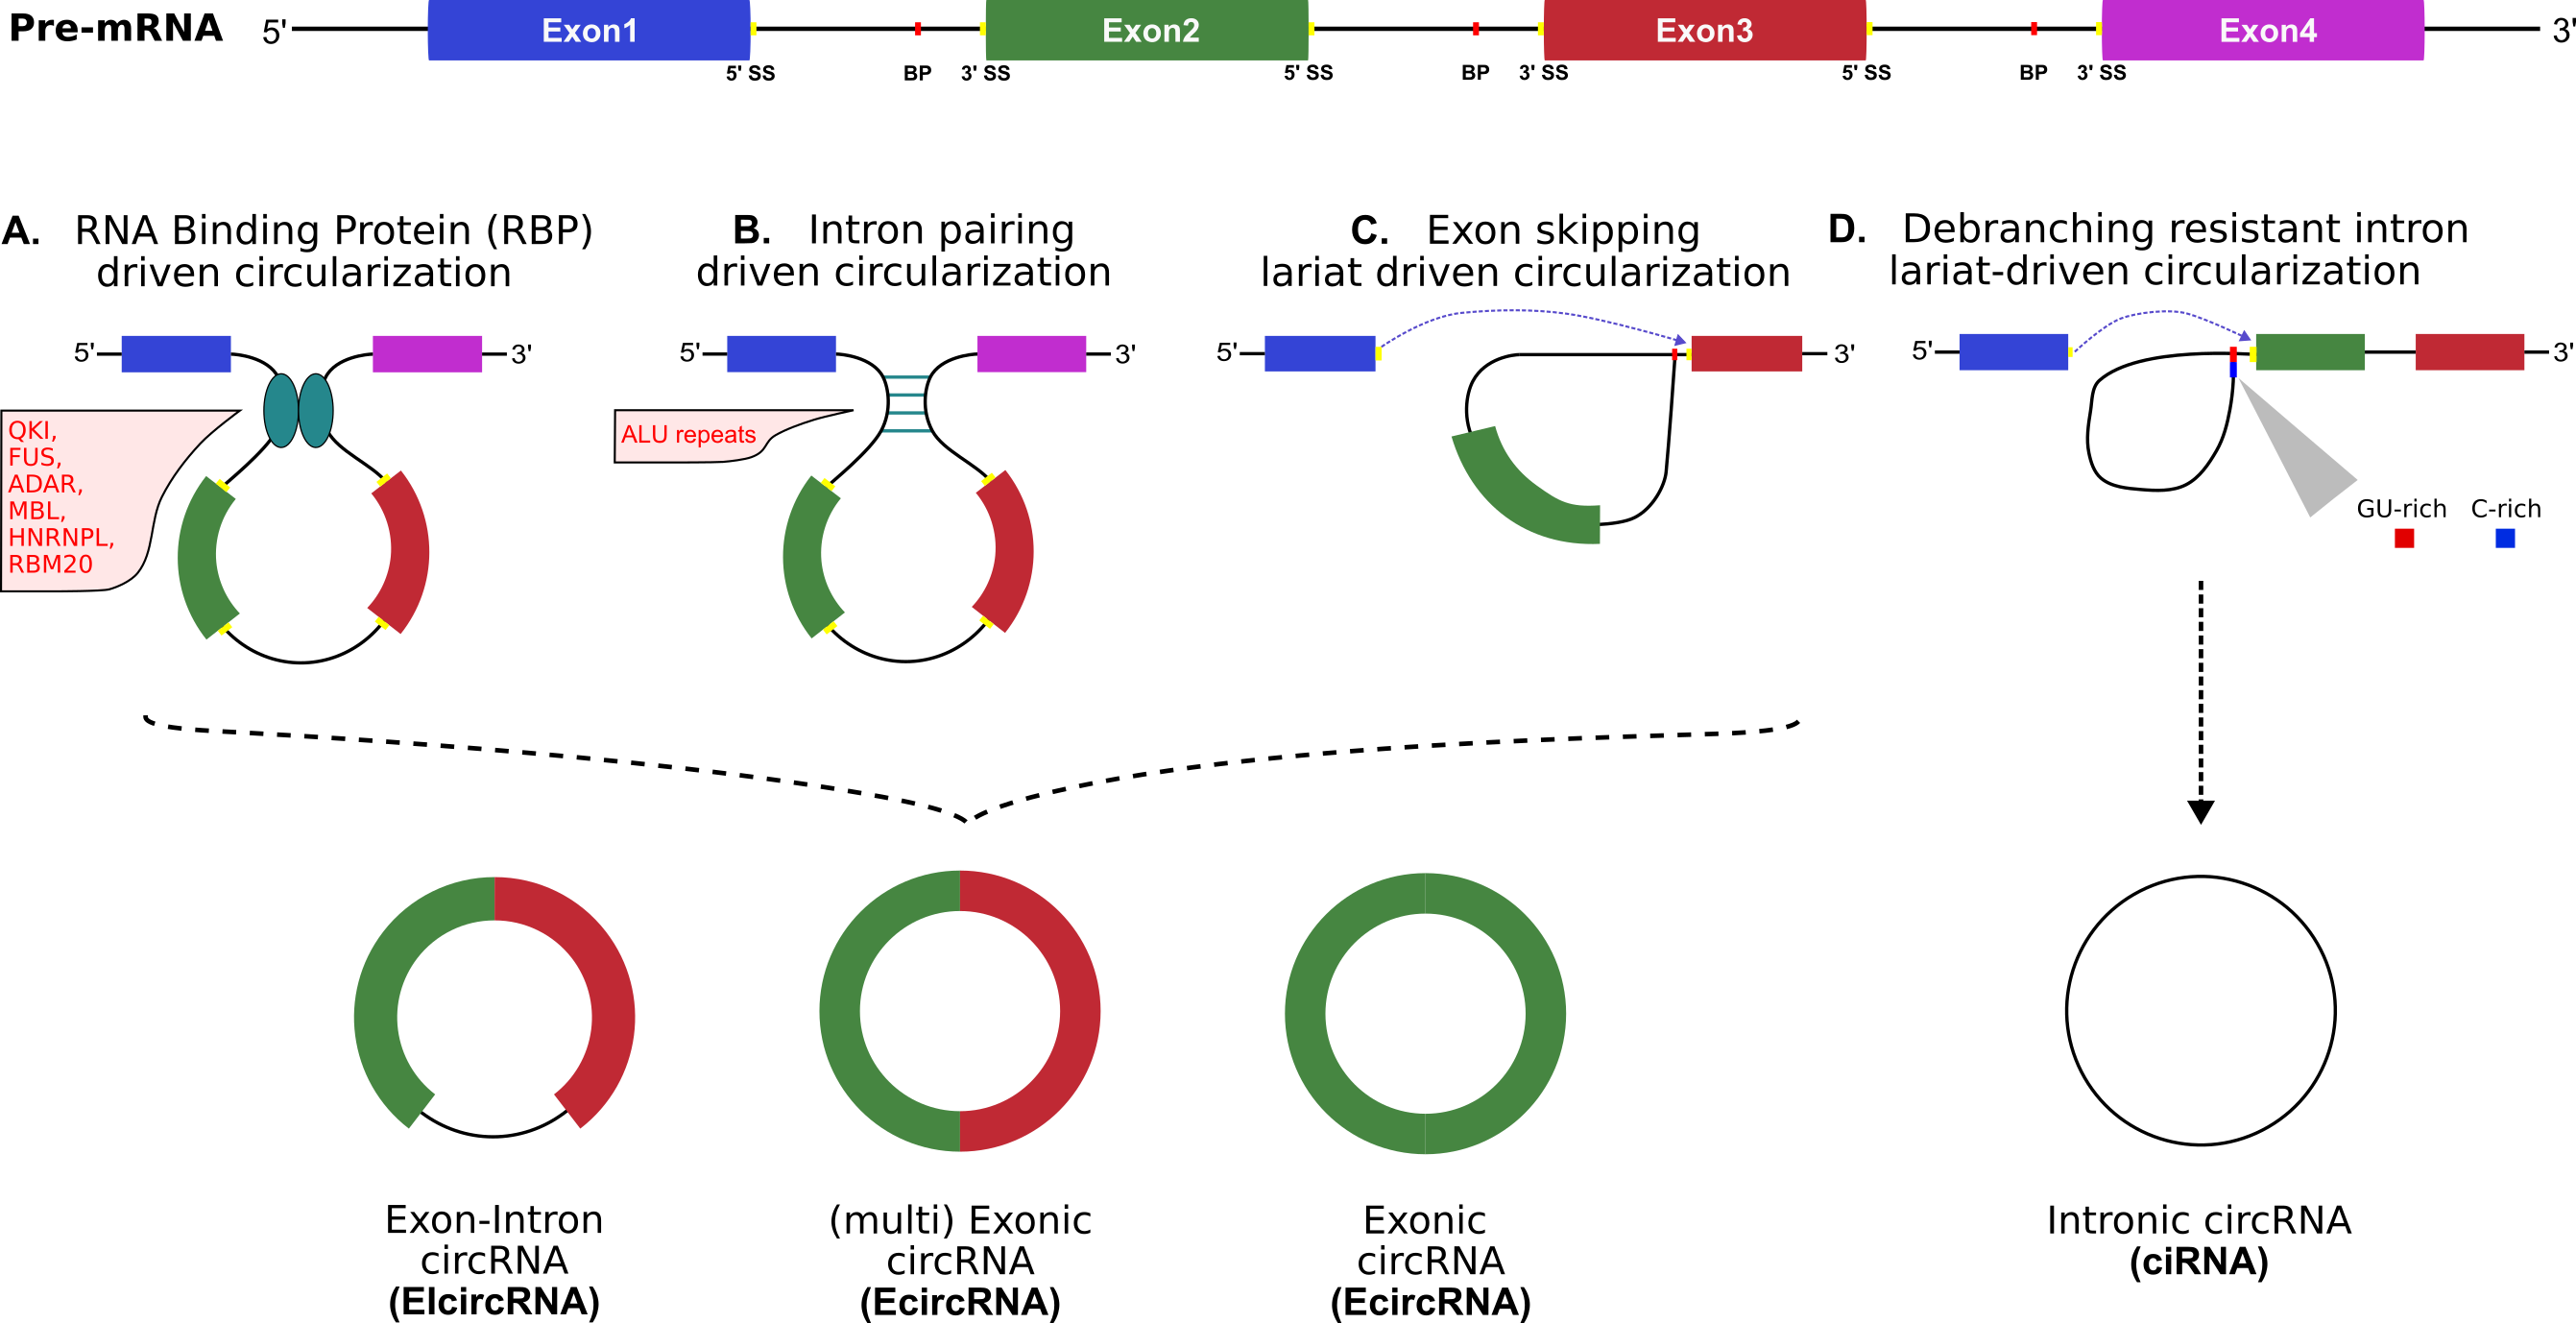
\includegraphics[width=\textwidth]{Chapter1/Figures/Figure1.png}
        \caption[Biogenesis of circRNAs]{\textbf{Biogenesis of circRNAs}. \textbf{A}: RNA binding protein circularization, \textbf{B}: Reverse-complementary matching sequence circularization e.g ALU repeats in humans, \textbf{C}: Lariat-driven circularization, \textbf{D}: Intron lariat circularization. Back-splicing processes \textbf{A, B} and \textbf{C} may undergo additional splicing to remove intronic or exonic sequences.}
        \label{biogen}
    \end{center}
\end{figure}

circRNAs' unique covalently closed loop structure lacking 5' and 3' tails confers resistance to RNase R degradation, granting them a much higher half-life than their linear mRNA counterparts \cite{Suzuki2006May, Enuka2016Feb}. This feature makes circRNAs an attractive biomarker in disease-based settings, with reports of circRNAs exhibiting differential expression in gastric, colorectal, ovarian and lung cancers, and enzalutamide resistant LNCaP cell lines \cite{Li2015Apr, Bachmayr-Heyda2015, Lim2021Dec}. Furthermore, circRNAs can be packaged and exported from the cell to bodily fluid via exosomes \cite{Li2015Aug, Shi2020Mar} facilitating the use of non-invasive liquid biopsies to monitor disease progression \cite{Wang2019Feb, Wu2023Apr, Pan2019Nov, Li2020Mar, Chen2020Apr, Louis2019Nov}. The mechanism of circRNA degradation and clearance remains an active area of research. Studies have found that miRNAs can facilitate the degradation of circRNAs via Argonaute 2 (Ago2)-mediated degradation supporting the hypothesis of circRNAs as active members in the ceRNA network \cite{Hansen2011Sep}. Other works demonstrate RNase H1-mediated degradation of ciRNAs with high GC content \cite{Li2021Nov} and the degradation of circRNAs containing m\textsuperscript{6}A modifications via endoribonucleolytic cleavage \cite{Park2019May}. 

\subsection{Principles and challenges for circRNA identification}

\begin{figure}
    \begin{center}
        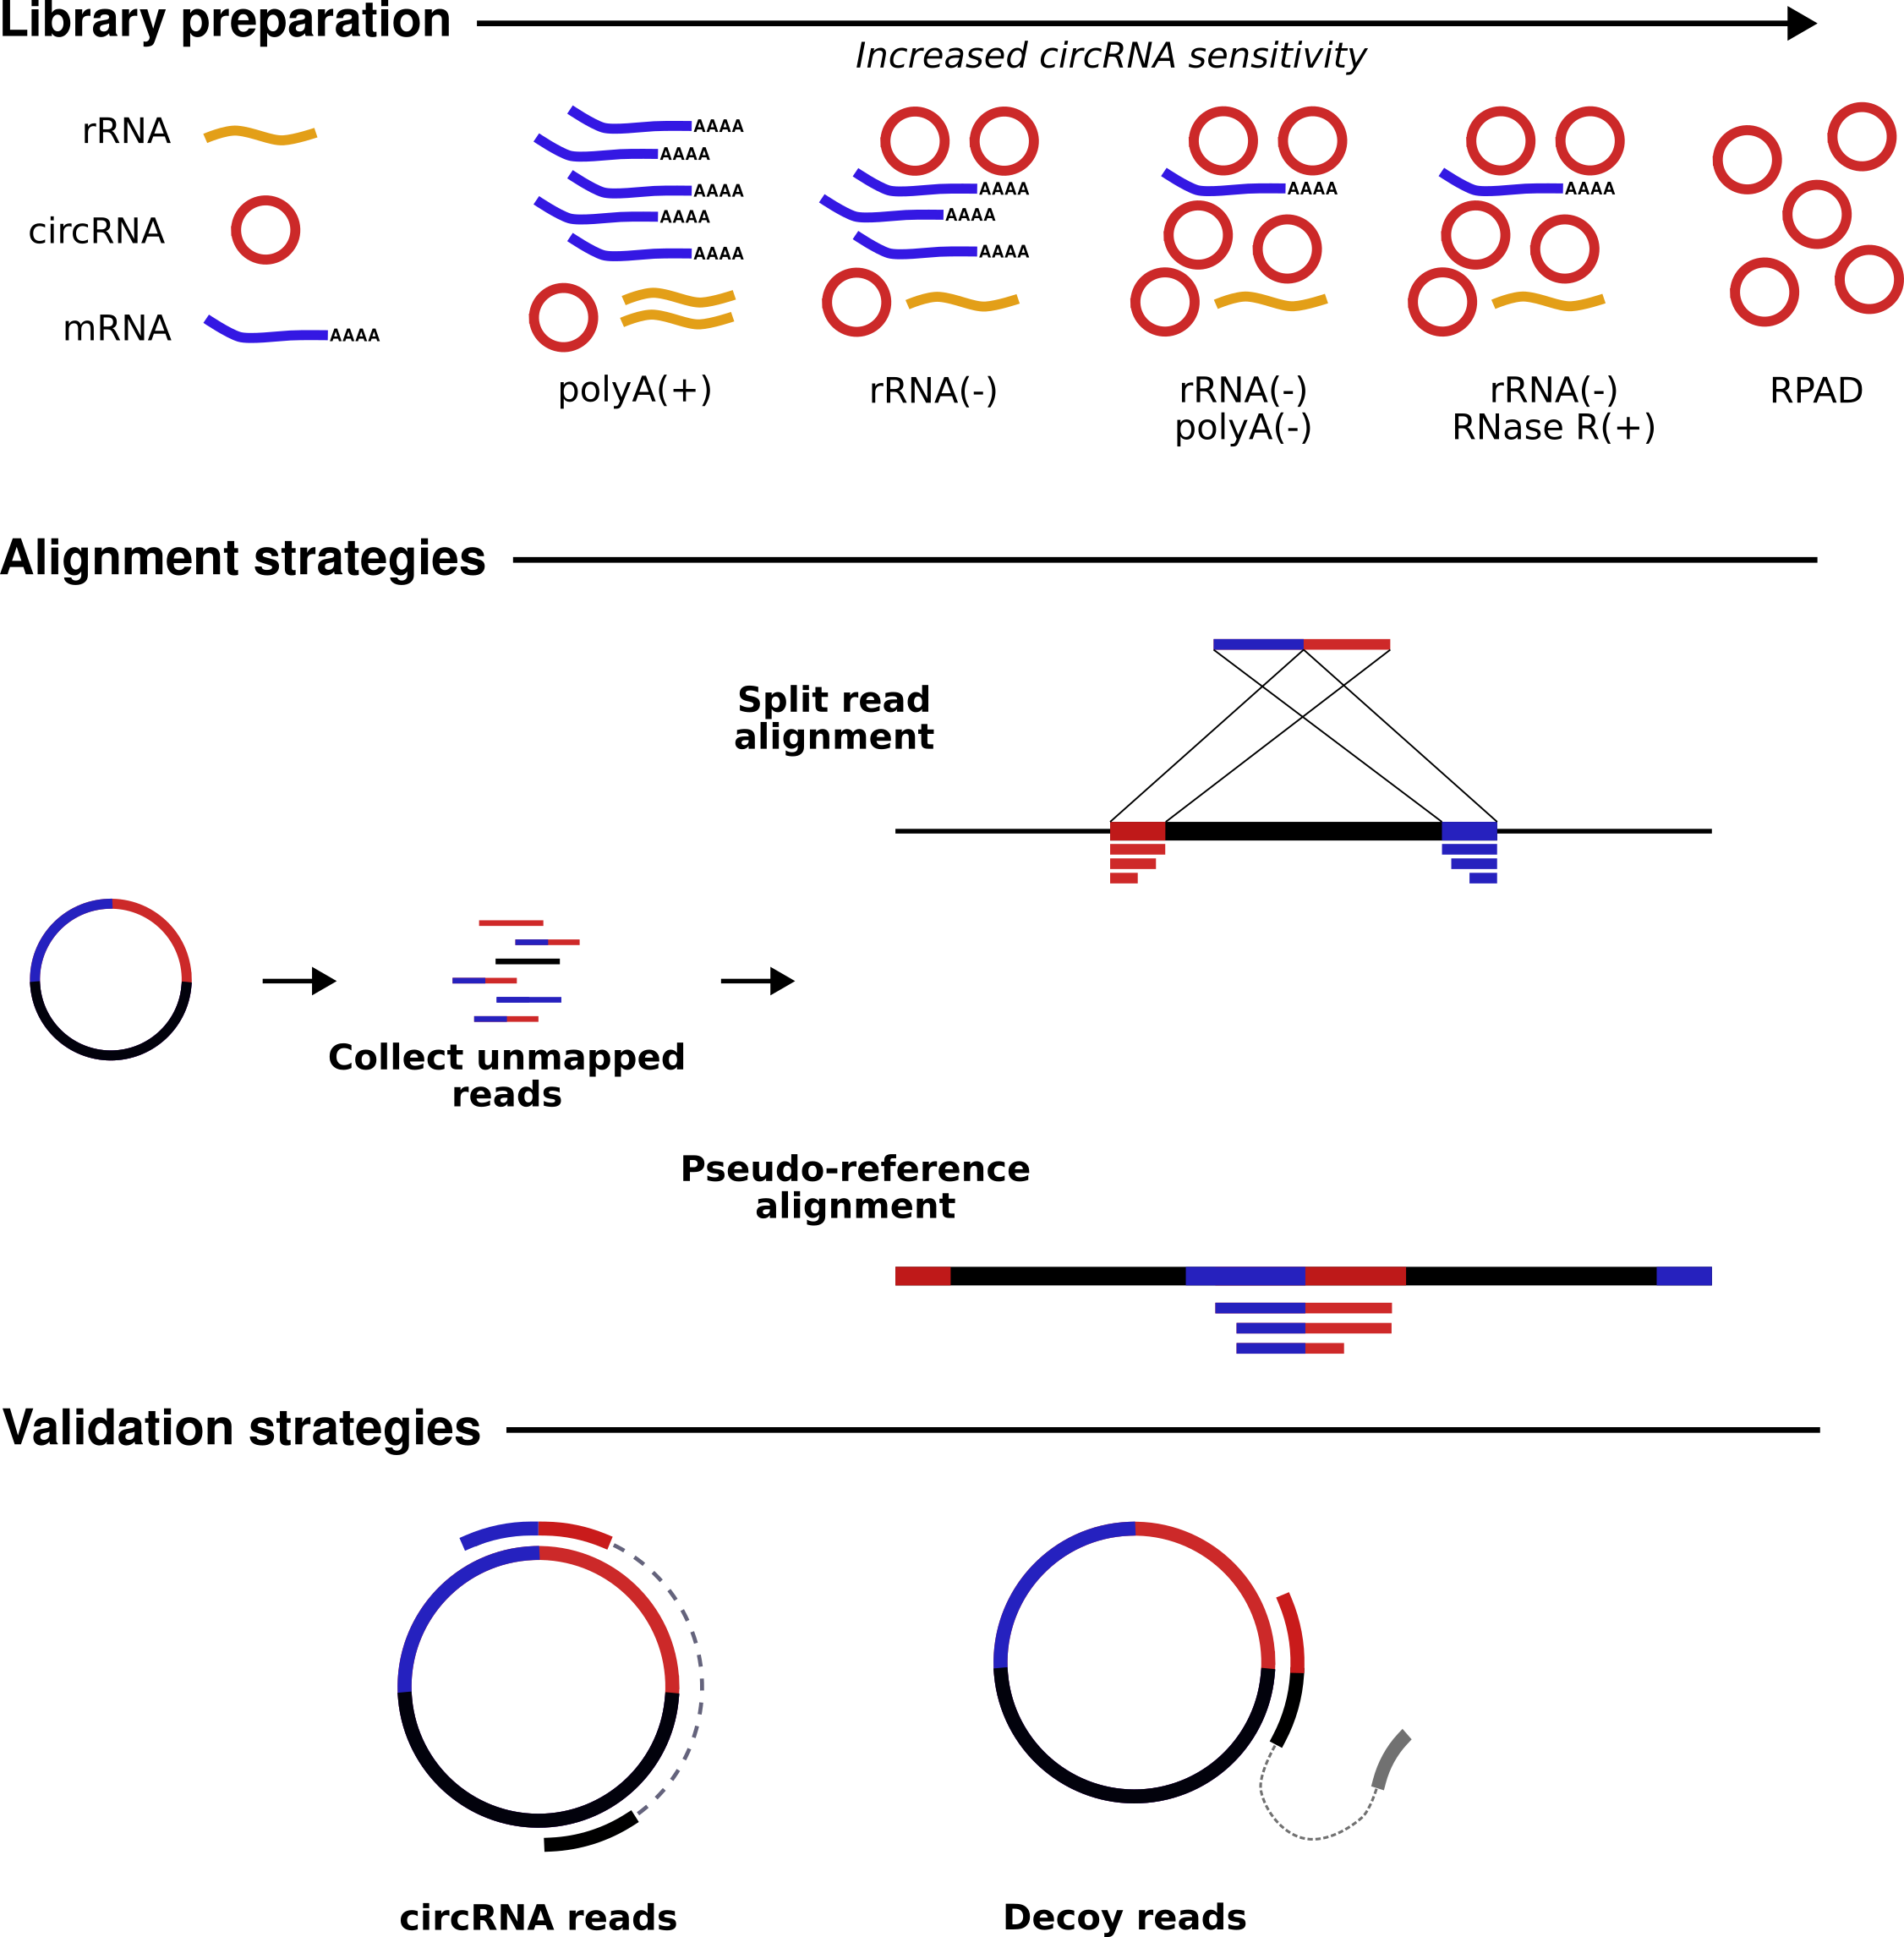
\includegraphics[width=\textwidth]{Chapter1/Figures/Figure2.png}
        \caption[Advancements in biochemical and bioinformatics strategies for circRNA detection]{\textbf{Advancements in biochemical and bioinformatics strategies for circRNA detection}. \textbf{Library preparation}: Left to right, in order of increasing circRNA capture sensitivity; poly(A)(+): unsuitable for circRNA detection, preferentially selects mRNAs; rRNA(-): ribosomal RNA depletion yielding a library with circRNAs and mRNAs; rRNA(-) \& poly(A)(-): ribosomal RNA depletion in conjunction with polyadenylation and depletion of poly(A) transcripts; rRNA(-) \& RNase R(+): ribosomal RNA depletion in conjunction with RNase R ribonuclease treatment depleting mRNAs; RPAD: RNase R treatment followed by polyadenylation and poly(A)\textsuperscript RNA depletion, yielding a highly pure circRNA library. \textbf{Alignment strategies}: Unmapped reads to the reference genome can be used to perform split alignment to identify reads aligning in opposite directions, or to map reads to  a BSJ pseudo-reference. \textbf{Validation strategies}: Paired-end sequencing greatly reduces false-positives, mates that map across the BSJ whose mates reside within the same transcript are indictive of circRNAs.}
        \label{artefacts}
    \end{center}
\end{figure}

\subsubsection{Library preparation}
circRNAs represent approximately 1\% of the transcriptome pool when compared to poly(A) RNA molecules \cite{Salzman2013Sep}, requiring novel strategies to enrich circRNA libraries prior to sequencing (Figure \ref{artefacts}). A typical eukaryotic RNA-Seq library preparation protocol involves the preferential selection of RNAs with poly(A) tails or the depletion of ribosomal RNAs (rRNAs). Due to circRNAs' covalently closed loop structure, poly(A) selection in libraries will almost completely remove all circular transcripts in a sample. By contrast, circRNAs are retained in rRNA-depleted samples and are enriched in samples treated with ribonuclease R (RNase R) to deplete linear RNAs. Random priming is preferred to oligo(dT) priming, as the former generates random oligonucleotide sequences for cDNA synthesis independent of poly(A) sequences, whilst the latter will generate libraries biased towards linear RNAs. One method, termed `RNase R treatment followed by polyadenylation and poly(A)\textsuperscript{+} RNA depletion' (RPAD) has emerged as a leading candidate for circRNA library preparation yielding the highest number of circRNAs and the highest sensitivity in a benchmark study \cite{Shi2022Dec}. RPAD employs the sequential depletion of linear RNAs via RNase R treatment, polyadenylation of remaining linear RNAs and a final round of poly(A)\textsuperscript{+} depletion using oligo(dT) beads followed by ribosomal RNA (rRNA) depletion to yield a high concentration circRNA library for sequencing \cite{Panda2017Jul, Pandey2019Feb}. In the absence of the RPAD method, rRNA depletion or RNase R\textsuperscript{+} are sufficient for generating RNA-Seq datasets for circRNA detection and have been used in benchmark studies analysing the performance of circRNA identification tools \cite{DCC}.

\subsubsection{Sequencing artefacts}
Technical artefacts introduced during sequencing can lead to the generation of false positives during circRNA identification. Reverse transcriptase, an enzyme used to synthesise complementary cDNA strands can undergo a template-switching event when brought in close proximity to a different RNA template with a suitable region for priming \cite{Cocquet2006Jul}. The original, incomplete synthesized strand is carried to the newly `switched' cDNA template where reverse transcriptase continues generating a chimeric molecule capable of mimicking alternative splicing and backsplicing. Alarmingly, these template switching events can account for up to 35-55\% of the isoforms computationally detected for a gene \cite{Roy2015}. Sequencing libraries that use adapter-ligation steps are at risk of generating chimeric sequences -- albeit at a much lower level. Finally, incorrectly called bases at the beginning or end of exons in genes containing highly homologous sequences can generate false positive splice site signals (GU/AG, etc.) \cite{Salzman2014Jun}. With respect to circRNAs, these sequencing errors can lead to sites that are mistakenly identified as backsplice sites when identifying circRNAs in samples. Due to the low levels of circRNA expression in cells when compared to other RNA transcripts, the presence of sequencing artefacts cannot be overcome by simply applying a read depth filter to quantification results. circRNA identification tools typically require paired-end data to overcome this source of error by requiring read 1 to map to the back-splice junction (BSJ) and its corresponding read 2 pair to map in the same transcript within a fixed distance \cite{Salzman2012}.

\subsubsection{BSJ-based circRNA identification}
The main step of any circRNA analysis is the identification of circRNAs in RNA-Seq datasets. This analysis is predicated on the detection of the BSJ, i.e the scrambled exon junctions representing the joining of an upstream 5' donor site to the downstream 3' acceptor site to form a circular structure. The majority of circRNA identification tools can be classed as one of two sub-groups: segmented-based-approach, whereby anchors (fixed-length segments taken from the end of reads) are extracted from unmapped sequencing reads and re-mapped to the genome; or pseudo-reference based in which a custom database of manually curated BSJ sites are generated and used to map the sequencing reads (Figure \ref{artefacts}). The first strategy allows for \textit{de novo} circRNA identification whilst the second is constrained to exons contained within the reference annotation file used for constructing the pseudo-reference database. As circRNA identification tools evolved, developers began to blend the two approaches and incorporate BSJ sequence context to optimize the process of circRNA identification (Table \ref{circtools}). \par
The first circRNA identification analysis performed by Salzman et al. (2012) \cite{Salzman2012} used the pseudo-reference based approach to identify circRNAs in ALL samples. Reads that mapped contiguously to RefSeq annotated genes using Bowtie \cite{Bowtie} were considered representative of linear transcripts and removed from the analysis. Subsequently, the RefSeq database was used to create a custom database of all intragenic exon-exon junctions against which reads that failed to align were mapped. An exon scrambling event was flagged if read 1 mapped to a non-canonical exon-exon junction as defined by the custom RefSeq database and read 2 mapped within the same transcript. The number of reads spanning the scrambled exon junction was used to estimate the relative abundance of candidate circRNAs. In contrast to the pseudo-reference based approach, the first tool created for the purpose of circRNA detection `find\_circ' \cite{findcirc} utilises the segmented-based approach. Firstly, paired-end reads are aligned to the genome to extract reads that do not contiguously align. A customised script then splits unmapped reads to obtain 20 nucleotide anchor sequences originating from the 5` and 3` ends of the reads. The anchors are re-aligned to the genome, with anchors mapping in reverse orientation extended to identify the breakpoint site in the anchor. The resulting BED file is filtered using the following criteria to arrive at a set of circRNAs: 1) splice sites must be flanked by GU/AG signals; 2) unambivalant breakpoints; 3) less than 2 mismatches in the extension procedure; 4) breakpoint cannot reside more than 2 nucleotides inside the anchor; 5) more than 2 reads must support the BSJ site and 6) splice sites must not be more than 100Kb apart. \par
UROBORUS \cite{UROBORUS} adopts a similar approach to `find\_circ', collecting and extracting 20bp anchors from reads that failed to map contiguously to the reference genome using TopHat. Anchor segments representative of a circRNA BSJ site mapped in reverse orientation within the same transcript with an overhang of $>$20bp at either end of both segments are termed `balanced mapped junctions' (BMJ) whilst segments with an overhang $<$20bp in one read are termed `unbalanced mapped junctions' (UMJ) and subject to different extension strategies. Both BMJ reads are separately extended outwards to the nearest splice-site to form paired-end segments, whilst for UMJ reads, the shorter mate is discarded and the single mapped seed is outwardly extended to the nearest splice-site (an extension distance must not exceed the length of the read minus 3bp). Bowtie is then used to remap the paired-end and single extended segments; segments aligning to the reference genome in the opposite orientation with read support $>$2 as detected by the UROBORUS algorithm are representative of circular candidates. \par
Post-transcriptional exon shuffling finder (PTESfinder) \cite{PTESfinder} combines the segment-based approach with the pseudo-reference based approach to identify circular candidates using Bowtie. Briefly, 20bp segment anchors are extracted from the ends of input sequencing reads and mapped to the reference transcriptome. Anchors that map to the same gene but in an inverted orientation are identified and used to construct a pseudo-reference (termed `PTES constructs') by concatenating the last 65bp of the underlying 5' exon and the first 65bp of the 3' exon. Reads are then aligned to the PTES construct, as well as genomic and transcriptomic references in order to generate mapping scores for circular candidate filtering. Candidates are marked as circRNAs when they exhibit high mapping scores to the PTES construct and low scores to the genomic and transcriptome reference. \par 
The concept of mapping reads to genomic, transcriptomic and BSJ databases to filter circRNA candidates was further improved upon by KNIFE \cite{KNIFE}. KNIFE maps reads to rRNA sequences, genomic, transcriptomic and a customised BSJ reference database using Bowtie2 \cite{Langmead2021}, discarding candidates that map with high scores to databases other than the custom BSJ reference. Where paired-end RNA-Seq data is available, the candidate reads spanning the BSJ site are subsetted into circRNA and decoy reads based on mapping information available in order to mitigate against false-positive BSJ reads generated by sequencing errors. For reads that fail to map to any of the databases, a \textit{de novo} analysis is performed using Bowtie coupled with a segment-based approach whereby segments are used to construct a \textit{de novo} index. The unmapped reads are then re-aligned to the \textit{de novo} index using Bowtie2 with the same criteria for pseudo-reference based alignment. KNIFE is one of the first circRNA identification tools to employ a statistical framework by obtaining a posterior probability for each circRNA candidate to predict if it is a true positive by using a logistic generalized linear model (GLM) based on the alignment features of read 1. In contrast to the circRNA identification tools discussed thus far which require extracting anchor sequences to identify putative BSJ sites using Bowtie or Bowtie2, both BWA \cite{BWA} and STAR \cite{STAR} are capable of directly detecting breakpoint events and chimeric fusions during read alignment. circRNA identification tools utilizing BWA or STAR therefore circumvent the need to manually extract anchors for BSJ identification using customized scripts, streamlining the process of circRNA identification and reducing computational overheads. \par 
CircRNA Identifier (CIRI) \cite{CIRI} is one such tool that utilises BWA-MEM sequence alignment mapping (SAM) information to identify reads in which two segments of the read align in chiastic order termed `paired chiastic clipping' (PCC) signals. Subsequent filtering leveraging paired-end mapping (PEM) information, GU/AG splice signals and mapping rates to homologous sequences removes false positives to arrive at a set of high-confidence circRNAs. One shortcoming of CIRI is its handling of unbalanced junction reads. Unbalanced junction reads are segments of length $<$19bp which are ignored by BWA-MEM to prevent multi-mapping and erroneous mapping, therefore lacking the necessary alignment information in the SAM file for CIRI to detect PCC signals. CIRI uses a dynamic programming algorithm to re-map unbalanced junction reads to balanced junction reads originating from the same junctions detected in the first alignment step. This step is computationally expensive and leads to the generation of false positives, an area specifically addressed by its successor, CIRI2 \cite{CIRI2}. CIRI2 is more cautious when addressing unbalanced junction reads and balanced junction reads with low mapping quality by utilising a maximum likelihood estimation (MLE) based on multiple seed matching. The undetermined segment of a putative BSJ read is divided into \textit{n} seeds of length \textit{m} (for example, a 50bp segment divided into five seeds of length 10bp) to determine if the segment belongs to a forward splice region or a back-splice region. The matched-seed numbers derived from the back-splice region ($k$\textsubscript{1}) and the forward-splice region ($k$\textsubscript{2}) are compared to produce two possible results: $k$\textsubscript{1}$>$$k$\textsubscript{2} $=$ back-splice region, and $k$\textsubscript{1}$\leq$$k$\textsubscript{2} $=$ forward-splice region. Since its publication in 2018, CIRI2 has become one of the most popular circRNA identification tools and has since been subsumed by CIRIquant \cite{CIRIquant} which extends its functionality by creating a pseudo-reference based on circular candidates detected by CIRI2, against which candidate reads are re-aligned using HISAT2 \cite{Kim2019Aug}. In addition to improved alignment, CIRIquant performs RNase R correction, linear RNA quantification and automated differential expression analysis of circRNAs. The suite of CIRI, CIRI2 and CIRIquant tools are all capable of calculating the ratio of circRNA BSJ reads and linear mRNA reads at a junction (CIRI2 and CIRIquant output this directly) to delineate the splicing preference in precursor mRNAs. When compared between conditions of interest, users can delineate differential splicing patterns. \par
Sailfish-cir \cite{Sailfishcir} utilises the outputs of CIRI, KNIFE, circRNA\_finder \cite{circRNAfinder}, or circRNA coordinates in BED format to transform candidate circular transcripts to pseudo-linear transcripts. Using the Sailfish model \cite{Patro2014May}, Sailfish-cir estimates the expression of both linear and circular transcripts spanning the pseudo-reference. Users should be aware that Salifish-cir does not report BSJ counts, but rather outputs transcripts per million (TPM). Given that both linear and circular TPM estimates are given for a junction, the circRNA junction ratio can be calculated manually. \par
ACFS \cite{ACFS} is another identification tool that uses BWA, however, its approach to circRNA identification is somewhat unorthodox. ACFS converts paired-end data to single-end data and collapses the reads prior to alignment, borrowing a strategy commonly used for miRNA alignment and quantification. After identifying candidate reads containing segments mapping in inverse orientation, ACFS uses maximum entropy models to predict the underlying BSJ sequence most likely to be generated by splicing. The advantage of this approach is that non-canonical dinucleotide splice sites are considered. The authors also point to the tool's ability to detect fusion circRNAs generated by chromosomal translocation events. This raises the question as to how ACFS controls for sequencing artefacts which can mimic fusion events - particularly when the tool discards paired-end read information. \par
circRNA\_finder and CIRCexplorer \cite{CIRCexplorer} were the first tools to use the outputs from the STAR aligner to identify circRNAs. STAR is capable of directly detecting and writing chimeric reads to the output binary alignment map (BAM) file or separately to a junctions.out tab-separated text file when `--chimSegmentMin' is set to a positive integer. Both circRNA\_finder and CIRCexplorer take advantage of the lightweight junctions.out file which contains within each line the genomic coordinates and CIGAR flags corresponding to each read segment that comprise the chimeric RNA molecule. circRNA\_finder imposes filtering on the putative circRNAs, allowing at most 3 mismatches, uniquely mapped reads, a maximum distance between splice-donor sites of 100kb and the condition that if one read spans the BSJ site, its mate should reside within the interval between the splice donor and acceptor site. Interestingly, CIRCexplorer does not impose such filtering strategies. It instead benefits from using an input reference gene annotation file to annotate putative circRNAs, thereby constraining results to exon-exon boundaries contained within the reference file, reducing the rate of false-positives. CIRCexplorer was superseded by CIRCexplorer2 \cite{CIRCexplorer2}, adding a suite of new modules for circRNA identification including alignment using TopHat-Fusion \cite{TopHatFusion}, annotation of circRNAs, \textit{de novo} assembly of novel circRNAs, characterising alternative-splicing events within circRNAs and support for parsing BWA, MapSplice \cite{MapSplice}, STAR and Segemehl \cite{segemehl} outputs. The deprecation of TopHat and TopHat-Fusion has resulted in CIRCexplorer2 largely becoming a tool for the downstream parsing and annotation of outputs from BWA, MapSplice, Segemehl and STAR. DCC \cite{DCC} is yet another circRNA identification tool that harnesses the power of the STAR aligner. In its recommended workflow, paired-end mates are mapped using STAR and each individual mate is processed in the same manner, generating three output files per sample -- joint mapping, mate1 and mate2 junctions.tab files. \par
DCC also offers a junction ratio test using CircTest to formally test variation in expression between circRNAs and their parent gene. We have noted that the sensitivity of circRNA identification tools using STAR can be drastically increased by implementing STAR 2-Pass mode, in which the chimeric junctions detected in all samples during the first mapping stage can be collected and incorporated into the reference genome on the fly during the second pass mapping stage for a sample. This method comes at the cost of increased false positives \cite{Engstrom2013Dec} and as such we recommend users adopt an ensemble approach or set suitably strict filtering parameters on detected circRNAs when employing STAR 2-Pass mode with circRNA\_finder, CIRCexplorer2 or DCC. \par
Finally, there exist splice-aware aligners that are capable of directly handling unmapped reads for detecting circRNAs during the alignment step. Non-co-linear scan (NCLscan) \cite{NCLscan} and Segemehl are two popular tools for this task, however, as NCLscan uses the proprietary aligner Novoalign, it's use is dependent on an active Novocraft licence. For this reason, Segemehl is considered the more popular tool in academic circles and has been incorporated into CIRCexplorer2 and intergration-based tools.

\subsubsection{Integration-based identification methods} \label{Integration-based identification methods}
A study by Hansen et al. (2016) \cite{Hansen2016Apr} highlighted the discrepancies in results generated by the most popular circRNA identification tools at the time (circRNA\_finder, CIRCexplorer, CIRI, find\_circ and MapSplice). Strikingly, only 854 circRNAs were identified by all tools out of the 5071 unique circRNAs detected, indicating that the choice of circRNA identification tool drastically impacts analyses. Furthermore, the use of RNase R\textsuperscript{+} and RNase R\textsuperscript{-} libraries from the same samples permitted the calculation of false positives returned by each tool. By analysing each paired combination of circRNA identification tools, the authors show that circRNA\_finder + CIRI had the highest rate of false positives (12.9\%), whilst circRNA\_finder + MapSplice achieved the lowest false-positive rate amongst analysed pairs (8.3\%). Perhaps the biggest takeaway from the study was that the combination of all tools yielded a false positive rate of 6.56\%, trading increased precision at the cost of reduced sensitivity. In 2018 Hansen \cite{Hansen2018} performed the same analysis again, this time using 11 circRNA identification tools (ACFS, CIRCexplorer, CIRCexplorer2, CIRI, CIRI2, DCC, find\_circ, KNIFE, MapSplice and UROBORUS). Results echoed those from 2016, with Hansen providing the following key recommendation when adopting an ensemble approach: users should combine results from circRNA identification tools that utilise different aligners to avoid biases. One such example is circRNA\_finder and DCC, which both use the STAR aligner. These two algorithms are thus less suited for pairing as the false positives generated are likely to be inherent to the aligner used. The analyses performed by Hansen et al. set new standards for best practices surrounding circRNA detection, ushering in a new class of circRNA identification pipelines termed `integrated tools' in which the user can select one or multiple tools for circRNA identification analysis with an automated intersection of results based on user-defined parameters. \par
CirComPara, developed by Gaffo et al. (2017) \cite{CirComPara} represents the first integration-based identification tool offering users the choice of CIRI, CIRCexplorer (STAR, BWA or Segemehl) and find\_circ. Results are configurable by requiring detected circRNAs to have \textit{n} reads spanning their BSJ site or circRNAs to be called by at least \textit{n} tools. Requiring only input sequencing reads, a reference FASTA file and a reference annotation file, the workflow streamlines the process of circRNA identification for users by automatically generating the required genome indices, reformatting reference annotation files and executing scripts for the analysis. The authors have also made the considerable effort to create a docker container with all of the necessary software for the analysis included, circumventing the need to install any tools from source. Gaffo et al. made substantial upgrades to CirComPara in 2022 by releasing CirComPara2 \cite{CirComPara2}. In addition to offering updated circRNA identification tools to the user (CIRI2, CIRCexplorer2 (BWA, Segemehl, STAR, TopHat), DCC and find\_circ), the workflow includes an improved expression estimate step when consolidating results from multiple tools. In CirComPara, circRNA abundances from multiple methods were calculated using the median of library-normalized BSJ counts across tools. In CirComPara2, the authors identify, for each method, the number of unique reads spanning the BSJ site of a circRNA thereby preserving the information returned by each tool used. Similar to CirComPara, CirComPara2 is packaged in a docker container facilitating rapid execution for users. \par
Several other integration tools exist for circRNA identification \cite{circRNAwrap, DEBKS, circmeta, circRNAprofiler, FcircSEC}, however they operate by using as input previously generated results from circRNA identification tools, unlike CirComPara and CirComPara2 which produce results directly from raw sequencing reads. Another novel integration tool that works with raw sequencing data is nf-core circrna, a workflow for the quantification, miRNA target prediction and differential expression analysis of circRNAs \cite{Digby2023Dec}. The workflow takes as input raw sequencing reads, a reference FASTA, reference gene annotation file and performs all of the preprocessing steps and execution scripts required for a circRNA analysis using circRNA\_finder, CIRIquant, CIRCexplorer2 (STAR), DCC, find\_circ, MapSplice and Segemehl. Similarly to CirComPara, the user can specify custom filtering parameters dictating the intersection strategies used on results. With support for 18 species, the workflow additionally performs automatic miRNA target prediction using miRanda and TargetScan, and automated differential expression analysis of circRNAs between phenotypes of interest provided in an optional metadata file. Developed using nextflow DSL2, the workflow requires Java version $>$8, the latest version of nextflow and a container client which will automatically download software packages for each analysis step (Docker, Apptainer, Conda) facilitating rapid `out-of-the-box' deployment using a single command.

\subsubsection{Full circle reconstruction} \label{Full circle reconstruction}
The first iteration of circRNA detection tools discussed above are predicated on identifying circRNAs via the presence of BSJ reads in sequencing data. Whilst this is an effective method to detect and quantify circRNAs in RNA-Seq data, the underlying mature spliced sequence (i.e the internal structure) of circRNAs remained opaque. circRNAs are subject to internal splicing events and intron retention (EIcircRNAs), therefore assuming that all of the underlying exons are retained within a circRNA will lead to false positives when predicting their targets based on sequence alignment against miRNA and RBP databases. To overcome this limitation and elucidate circRNA isoforms, coverage of paired-end RNA-Seq reads through the circRNA are utilised to characterise read densities amongst exons within the circular transcript. \par
The first tool developed capable of delineating circular isoforms via \textit{de novo} construction of circRNA exons, CIRI-AS \cite{CIRI-AS}, was developed by the same group that produced CIRI2. Using the outputs from CIRI2 and a BAM file generated by BWA-MEM, the algorithm works by analysing local alignment positions of segments within candidate BSJ reads and its paired mate to identify forward spliced junctions representative of joined circular exons. For each circexon candidate, sequencing depth variation, BSJ read pair coverage and splice junctions from non-BSJ reads are taken into account. CIRI-AS can be performed without a reference GTF file, permitting flexible usage with non-reference organisms. In addition to detecting circexons, CIRI-AS can detect intronic or intergenic circRNA fragments (ICFs) when adequate sequencing depth is provided. CIRI-full \cite{CIRI-full} builds on CIRI2 and CIRI-AS for full resolution of circRNAs internal structure. The main premise of CIRI-full revolves around the detection of reverse overlap (RO) reads. During reverse transcription, the circular structure of circRNAs can cause continuous circumnavigation of reverse transcriptase within the circRNA, producing read pairs that overlap in reverse orientation. Moreover, the presence of a 3'-RO overlap in both RO reads indicates the full circle has been transcribed facilitating full circRNA reconstruction. For RO reads that do not overlap due to insert size length, CIRI-full borrows information from CIRI2 (BSJ sites) and CIRI-AS (circexons) to produce a reconstructed circRNA. Next, a forward-splice graph (FSG) is constructed by assembling BSJ and RO reads within a detected circRNA BSJ site to model the read coverage of each path using Monte Carlo simulations, providing resolution of circRNA isoforms. \par
Full characterization of circRNAs (FUCHs) \cite{FUCHS} is yet another tool capable of detecting circular isoforms, accepting as input results from  circRNA\_finder, CIRI2, CIRCexplorer2, and DCC in conjunction with a BAM file containing chimeric reads, linear reads and unmapped reads. The first step is to isolate circular reads from the BAM file, then identify splicing events within the circular transcript by detecting exon-skipping events in reads. The coordinates of the skipped exons are used to generate coverage statistics, assigning reads to one of two circular isoforms. The output files generated detail the circular candidate's genomic location coupled with read depth for each underlying exon. In this way, researchers can delineate the spliced transcript by removing exons with a read count of 0. \par

\subsubsection{circRNA identification using long-read sequencing}
Long-read sequencing technologies developed by Oxford Nanopore Technologies (ONT) or Pacific Biosciences (PacBio) are capable of producing sequencing reads several thousand nucleotides in length, providing full resolution of internal exon structure of linear transcripts \cite{Rhoads2015Oct,Deamer2016May,Byrne2017Jul,vanDijk2018Sep}. This technology represents a promising avenue for full circle reconstruction of circRNAs over short-read based algorithms which struggle to identify circRNA FSJ sites located at distance from the BSJ reads \cite{CIRI-AS,CIRI-full,FUCHS}. However, in most cases cDNA sequencing is performed using oligo(dT) primers which are unsuitable for circRNAs lacking poly(A) tails, therefore requiring an adaptation of the amplification step prior to sequencing. \par
IsoCirc \cite{isoCirc} is a strategy for characterising full-length circRNA isoforms using rolling circle amplification (RCA) followed by ONT sequencing. Here, samples are first treated with rRNA depletion and RNase R to deplete linear RNAs. Next, cDNA/circRNA double-stranded hybrids are generated using random hexamer priming in conjunction with reverse transcriptase, after which overhangs present in the cDNA circle are removed using Mung Bean endonuclease. The cDNA circle is then ligated using SplintR ligase to form a circular template for the generation of long concatemeric ssDNAs for sequencing via RCA. The strategy to generate concatemeric ssDNAs is a key step in the isoCirc protocol, as it allows for the generation of a final `consensus' circRNA sequence thereby minimising the error rates associated with ONT sequencing \cite{Jain2015Apr}. Computationally, the consensus circRNA sequence is generated using Tandem Repeats Finder \cite{Benson1999Jan}. Two copies of all consensus sequences that pass filtering are concatenated and used for downstream mapping to the reference genome via minimap2 \cite{Li2018Sep}. Subsequent filtering strategies are used to identify both the optimal alignment record per consensus sequence and the optimal consensus sequence per long read. Only candidate circRNAs with high quality BSJ and FSJ sites are reported as full-length circRNA isoforms, whilst single-exon circRNAs require only high confidence BSJ sites. \par
In contrast to the RCA amplification method employed by isoCirc, CIRI-long \cite{CIRIlong} utilises rolling circle reverse transcription (RCRT) to synthesise circRNA cDNA. First, circRNAs are enriched using a customised approach for RNA-seq library preparation. rRNA depletion is performed using a RiboZero kit followed by poly(A)-tailing prior to RNase R digestion to increase linear RNA degradation \cite{Xiao2019Sep}.
The remaining circRNAs in the library are amplified using random primers and SMARTer reverse transcriptase to initiate RCRT and cDNA synthesis. This step generates long cDNA fragments, within which exists multiple copies of full-length circRNA sequences. SMARTer sequencing adapters are added to each cDNA fragment to enable effective amplification in the absence of poly(A) tails. Once cleaned circRNA reads have been obtained, CIRI-long has two main steps: 1) candidate circRNA identification and 2) isoform colapsing. Step 1 involves using \textit{k-mers} to search for repetitive sequences and the boundaries of circRNA fragments within the long reads. Next, a cyclic consensus sequence (CSS) for each read is generated using the SPOA library \cite{Vaser2017May}, with an 80\% similarity score as defined by the Levenshtein distance used to filter high-confidence circRNA candidates. CSSs of length $>$150bp are then mapped to the reference genome using minimap2, whilst shorter reads are mapped using BWA MEM. An iterative alignment strategy is used during CSS alignment, whereby unmapped segments residing in the head or tail region of the CSS are appended to the opposite end of the CSS. Subsequent realignment determines if the re-ordered CSS obtains better scores than the previous alignment. This iterative process converges once the transformed CSS is fully aligned to the reference genome with high scores. In step 2, candidate circRNA isoforms are detected by clustering reads based on their location within the reference genome. All sequences within a cluster are subject to hierarchical clustering based on pairwise sequence similarity, producing consensus sequences for each cluster representative of a circRNA isoform. \par

circFL-seq \cite{circFLseq} is another tool for detecting circRNAs using long reads, sharing similarities with CIRI-long in terms of library preparation and the generation of circRNA cDNA templates using RCRT. The bioinformatics component is divergent, relying on a pseudo-reference based approach after identifying consensus sequences. Reads are initially aligned to the reference genome using minimap2 to identify chiastic overlapping segments indicative of candidate circRNA reads (CCR). During this step, CCRs are classified as normal, fusion on same chromosome or fusion on different chromosome. The boundary of the chiastic segment of the CCR are used as a proxy for BSJs, and subsequently used to concatenate two sequences 150bp upstream to 150bp downstream of the BSJ to generate a pseudo reference sequence for each read. CCRs are then aligned against the pseudo reference, corrected using multiple aligned BSJ sites, reference annotations and canonical splicing motifs. Full length circRNAs are produced leveraging the BSJ and FSJ information for a given circRNA. circFL-seq offers two optional modules for low quality reads; \textit{De novo} self-correction (DNSC): consensus sequences of reads are detected using TideHunter \cite{Gao2019Jul}. Following removal of consensus sequences containing long repetitive elements using Tandem Repeats Finder \cite{Benson1999Jan}, a set of filtered consensus sequences are available for downstream processing. cRG mode: using the self-corrected CSs, RG mode is re-run using a query sequence of three copies of the corrected CS. The authors of circFL-seq found that cRG correction reduced the error rate of both indels and mismatches in the consensus sequence, and thus should be run for all deployments of circFL-seq.\par 

In comparisons between the tools \cite{circFLseq,Rahimi2021Dec}, the RCA method was shown to produce longer reads than the RCRT method (up to 50kb vs. 1kb). Whilst more expensive, the longer reads produced by the RCA method allow for error correction during the consensus sequence identification step. Of note, the ligation step by isoCirc may introduce false positives via the ligation of residual linear RNA or truncated circRNA cDNA fragments that are difficult to resolve computationally. The RCRT method coupled with anchor priming or template switching employed by circFL-Seq and CIRI-long, respectively, are more resistant to this issue. In a direct comparison using HEK293 cells and mouse brain tissue, circFL-Seq was shown to be more sensitive than CIRI-long (HEK293: 27869 vs. 15242; mouse: 18396 vs. 9258 known BSJ sites), with similar rates of precision \cite{circFLseq}. Conversely, in comparison with isoCirc with deep sequencing libraries, circFL-Seq was less sensitive than isoCirc (34046 vs. 79312 known BSJ sites). IsoCirc recovered far more circRNAs expressed at low levels (38846 vs. 2511, read count=1) indicating that whilst more expensive, isoCirc is the most sensitive method for detecting circRNAs from long-read sequencing.

\subsubsection{Machine learning circRNA identification}
circRNA biogenesis can be attributed to hallmarks within the flanking intronic regions: reverse complimentary matching (RCM) sequences \cite{Ivanov2015Jan} (also referred to as inverted repeats \cite{Dubin1995Dec}), and more specifically, ALU and tandem repeat motifs in humans \cite{Jeck2012Dec} facilitating the generation of RNA hairpin structures that bring distal splice sites within close spatial proximity. These hallmarks coupled with evolutionary conservation scores, secondary structure information and the density of single nucleotide polymorphisms (SNP) within conserved miRNA binding sites \cite{Thomas2014Aug} have been identified as predictive features for discriminating circRNAs from other classes of long non-coding RNAs (lncRNAs) using statistical and machine learning (ML) based approaches \cite{PredcircRNA,circDeep,StackCirRNAPred,CirRNAPL}. Released in 2015, PredcircRNA \cite{PredcircRNA} represents the earliest attempt at leveraging multiple layers of contextual sequence information to discriminate circRNAs vs. lncRNAs. The 188 features extracted from transcripts for training and testing the PredcircRNA model fall under one of four categories: 1) Graph features from RNA structures: nodes represent nucleotides and edges provide higher level information such as sequence backbone connection or bonds between base pairs \cite{GraphProt}. To reduce the dimensions of the graph Random Forest (RF) was applied to extract the top 101 features. 2) Sequence conservation scores were computed using PhyloP conservation tracks \cite{PhyloP}, wherein the mean, variance, and maximum conservation scores within each transcript were determined. Additionally, the authors calculated the cumulative successive conservation score and the frequencies of nucleotides surpassing binned score thresholds. 3) Component composition scores: tri-nucleotide composition, GC content, sequence length, the presence of GT, AG, GTAG and AGGT motifs were extracted. 4) ALU, tandem repeats, ORFS and SNP: genome tracks for ALU sites, ORF sequences and SNP sites were downloaded and qunatified at the transcript level. The 188 extracted features were ranked in terms of importance using RF, with conservation features, GT/AG motifs and component composition scores identified as the most influential features for circRNA classification. The authors next utilised three machine learning classifiers, RF, support vector machines (SVM) and multiple kernel learning (MKL) to predict circRNAs, with the MKL method providing the best results in both the training and the independent test sets. Similarly to PredcircRNA, circDeep \cite{circDeep} leverages sequence features to classify circRNAs. The authors developed three novel descriptors to classify circRNAs; 1) RCM descriptor: a \textit{H}-score which represents the presence of RCMs, 2) Conservation descriptor: utilising phastCons \cite{phastCons}, the maximum, mean and median value of averaged conservation scores per exon are calculated (intronic transcripts are treated as a single exon) in addition to analysing the number of successive bases whose scores are above a given threshold, and 3) Asymmetric convolutional neural network - bidirectional long short-term memory network (ACNN-BLSTM) descriptor: a deep learning model that learns the local sequence context of transcripts as well as long-range dependencies between sequence features learned by ACNN layers. Using each of these three descriptors, the authors developed a fusion model to combine the three heterogeneous modalities termed `feature fusion fine-tuned' which boasts greatly improved run times over PredcircRNA (largely due to the absence of GraphProt in the pipeline) and an impressive 12\% increase in accuracy. \par
A limitation of these methods is that splice site and back-splice junctions are ignored, focusing instead on surrounding sequence context and classification tasks delineating mRNAs vs. lncRNAs vs. circRNAs. Given the unique BSJ of circRNAs, it is key to understand the properties and relationships between splice sites that constitute canonical linear splicing and a circular back-splicing event. DeepCirCode \cite{DeepCirCode} analyzes the nucleotide sequences of two splice sites and predicts whether the two splice sites produce a back-splicing event characteristic of circRNAs. Briefly, the DeepCirCode model was trained using 50nt sequences surrounding each back-splicing instance in a custom dataset (back-splice sites detected by at least two computational methods present in circRNADb \cite{circrnadb} or circBase \cite{circbase}) and fed to a convolutional neural network (CNN). By leveraging the position weight matrices (PWMs) learned by DeepCirCode, users can predict the likelihood of a given sequence to produce a back-splicing event. Junction encoders and deep interation (JEDI) among splice sites \cite{JEDI} is a tool that optimizes a deep learning model for circRNA prediction in the absence of annotated back-splice sites as training data (zero-shot learning). Unlike its predecessors, JEDI is not limited to interrogating only two splice sites. In this way, it can model the sequence context and flanking regions of all splice sites within an transcript, making it an effective tool for classifying circRNAs that are derived from genes which also produce linear transcripts.\par
The latest addition to the suite of circRNA machine learning tools, CIRI-deep \cite{CIRIdeep}, infers differentially spliced circRNA (DSC) events between tissues/samples of interest in various types of datasets by leveraging the previously published Deep-learning Augmented RNA-seq analysis of Transcript Splicing (DARTS) framework \cite{DARTS}. Briefly, the CIRI-deep neural network model was constructed by running CIRIquant \cite{CIRIquant} on 397 filtered samples from RNA Atlas \cite{RNAAtlas} and CircAtlas \cite{circatlas} to obtain back-splice junction (BSJ) counts and forward-splice junction (FSJ) counts representative of cirRNA and linear mRNA reads spanning junction sites. Dataset labels were generated in a pairwise fashion using DARTS Bayesian Hypothesis Testing with an uninformative prior (DARTS BHT-flat) wherein the junction ratios were used to assign high-confidence differential or unchanged splicing events between samples. Next, 3527 relevant circRNA \textit{cis} sequence features were extracted in addition to the expression levels of 1499 \textit{trans} RBPs associated with circRNA biogenesis-related genes, splicing factors and RNA degradation enzymes. The design and underlying model employed by CIRI-deep offers a two-fold advantage for users: 1) By developing a model trained on approximately 25 million DSC events and both \textit{cis} and \textit{trans} factors, CIRI-deep can predict DSC events independent of BSJ reads by incorporating a Bayesian prior (DARTS BHT-info). This permits the usage of CIRI-deep on datasets with low replicates, low sequencing depth and 10X single cell or spatial transcriptomics datasets in which circRNA BSJ reads are sparsely detected. 2) CIRI-deepA, a variant of CIRI-deep, was trained on \textit{trans} RBP gene expression data from poly(A) selected datasets in RNA Atlas, permitting the detection of DSC events in large cohort datasets such as GTEx \cite{GTExConsortium2013Jun} and TCGA \cite{TCGA}. The authors of CIRI-deep conceed that the model is not without limitations, particularly in the context of cancer samples in which mutations to \textit{cis} elements and dysregulation of \textit{trans} factors are not suitable for use by a model trained on reference genomes. 

\subsubsection{Overview of computational challenges}
Hypotheses generated about the genome-wide role of circRNAs must be based on accurate quantification of circRNAs to mitigate the propagation of false positives in published literature. In this section, we discuss current computational methods used by researchers to arrive at a set of high confidence circRNAs.

\subsubsection{circRNA detection strategies}
Researchers should be aware that tools will generally fall under one of two categories: 1) segmented based circRNA detection or 2) pseudo-reference based circRNA detection. In the segmented based approach, unmapped reads (i.e reads that do not contiguously align to the reference) are collected and split into segments in order to identify reads that map to the back-splice junction. Whilst this method permits the discovery of \textit{de novo} circRNAs and is more suited for organisms with incomplete or poorly annotated reference genomes, the method is less sensitive \cite{Jeck2014May}. Researchers should therefore investigate the methods used by the quantification tool to mitigate these erroneous circRNA calls and if absent, apply filters manually. Possible methods for reducing false positives in segmented-based circRNA detection are: 1) Requiring the mate of a candidate BSJ read to be within a suitable distance and mapped within the same transcript. This method removes decoy reads generated by genomic rearrangements or sequencing artefacts that mimick the BSJ of circRNAs \cite{circRNAfinder}. 2) Filter BSJ sites to keep candidates that are flanked by canonical splice site motifs (e.g GU/AG) \cite{findcirc}. Alternatively, users can inlcude non-canonical splice sites in their search and apply a ranking system e.g GC/AG U2-type, AT/AC U12-type \cite{CIRIlong} in order to score \textit{de novo} circRNAs. 3) Enforce high quality mapping around the BSJ site, e.g requiring no more than \textit{n} mismatches, insertions or deletions in \textit{n}-bp each side of the BSJ junction. By combining metrics 2 and 3, researchers can produce a ranked list of circRNAs instead of applying hard filters. \par
For the pseudo-reference based approach, there are two methods by which a pseudo-reference database can be designed which will greatly influence the circRNAs detected by such a tool. The first method is to generate a database of all intragenic exon-exon junctions using the reference GTF/GFF file, thereby creating every possible combination of back-splicing events. This method is restricted to species that provide an annotated reference genome file and can only detect circRNAs that share splice sites with linear RNAs. The second method is more favourable to unannotated organisms, whereby circular candidates collected in the first alignment step are tandemly duplicated to construct a pseudo-reference circRNA transcriptome against which the circular candidate reads are mapped against. This method reduces the rate of false positives by requiring the circular candidate reads to be linearly and fully aligned to the BSJ region of the pseudo-reference \cite{CIRIquant,Sailfishcir,PTESfinder}. \par
Due to the discrepancies in the two approaches, high variance between sets of circRNAs called by individual tools inevitably develops due to computational `blind spots' inherent in each approach \cite{Szabo2016Oct}. Users will therefore be tempted to apply multiple circRNA quantification tools to their chosen dataset, particularly with the advent of integrated based tools \cite{RAISE,CirComPara,CirComPara2,Digby2023Dec,circRNAwrap}. Whilst combinatorial approaches to circRNA identification will greatly increase the precision of the results, users should be aware that the sensitivity of different tool combinations will vary greatly \cite{Hansen2016Apr,Szabo2016Oct,Hansen2018,Zeng2017Jun,Vromman2023Aug}.

\subsubsection{circRNA identification tools exhibit high variance}
Perhaps the most striking statistic that researchers will encounter when employing one or more circRNA quantification tools is the disparity in agreement amongst tools. Whilst individual tools have been shown to exhibit high precision, their ability to detect all true positive circRNAs in the benchmarking pool (i.e sensitivity) fluctuates \cite{Vromman2023Aug,Zeng2017Jun}. We describe three publications: Zeng et al. (2017) benchmarking 11 circRNA identification tools individually \cite{Zeng2017Jun}; Gaffo et al. (2022) benchmarking combinations of 7 circRNA identification methods \cite{CirComPara2} and Vromman et al. (2023) benchmarking 16 circRNA identification tools in conjunction with orthogonal validation techniques \cite{Vromman2023Aug} to highlight this point. \par

\paragraph*{Zeng et al. 2017}
The authors evaluated CIRCexplorer \cite{CIRCexplorer}, circRNA\_finder \cite{circRNAfinder}, CIRI \cite{CIRI}, DCC \cite{DCC}, find\_circ \cite{findcirc}, KNIFE \cite{KNIFE}, MapSplice \cite{MapSplice}, NCLScan \cite{NCLscan}, PTESFinder \cite{PTESfinder}, Segemehl \cite{segemehl} and UROBORUS \cite{UROBORUS} circRNA identification tools in order to assess the precision, sensitivity, F1 scores and AUC of each tool in both simulated and real datasets. In a simulated positive dataset containing 14689 HeLa circRNAs deposited in circBase \cite{circbase}, most tools achieved high precision ($>$94\%). However, the sensitivity of each tool varied, ranging from 52\%-93\%. The authors then calculated the harmonic mean of precision and sensitivity (F1 score) to determine the best performing tools. Only four tools had an F1 score $\geq$0.9 --- KNIFE (0.96), CIRI (0.92), PTESFinder (0.91) and Segemehl (0.91). KNIFE was the best performing tool in the simulated positive dataset, capturing 92\% of the available circRNAs at a precision rate of 99.66\%. \par

The authors then generated a background simulated linear RNA dataset to assess the fraction of false positive circRNAs called by each tool (NCLScan was omitted due to its inability to construct a noncollinear reference from linear reads). Alarmingly, Segemehl (1084), find\_circ (712), UROBORUS (620) and KNIFE (554) called a high rate of false positive circRNAs in the background dataset. The simulated positive dataset was then added to the background dataset to generate a mixed dataset. Interestingly, Segemehl (87\%), UROBORUS (88\%) and find\_circ (92\%) exhibited dramatic drops in precision compared to the positive dataset analysis, whilst all other tools achieved precision rates above 96\% in the mixed dataset. NCLScan boasted impressive precision rates in each dataset (99\%) however this score is undermined by the fact NCLScan detected only $\sim$7740 circRNAs from the pool of 14689, reflected in poor sensitivity scores (52\% positive and mixed). Using the simulated datasets the authors have demonstrated the underlying variance in sets of circRNAs called by each tool, underpinning the fact each tool has its own blind spots. \par

Next, the authors obtained HeLa RNaseR\textsuperscript{-}, HeLa RNaseR\textsuperscript{+} and Hs68 RNaseR\textsuperscript{-}, Hs68 RNaseR\textsuperscript{+} datasets with the goal of identifying the percentage of `true circles' detected by tools in RNase R\textsuperscript{-} samples i.e called circRNAs that were not then depleted in RNase R\textsuperscript{+} samples. MapSplice, which had shown high precision and relatively poor sensitivity in the simulated datasets captured the highest percentage of true circRNAs (54\% HeLa, 76\% Hs68) indicating that whilst conservative, MapSplice captures a high proportion of true positives. Finally, the authors identified the top 100 expressed circRNAs identfied by each tool in the RNase R\textsuperscript{-} datasets to ascertain if high BSJ read counts are a reliable proxy for `true circles' as performed by Hansen et al. 2016 \cite{Hansen2016Apr}. In the HeLa dataset, KNIFE (75), CIRCexplorer (73), CIRI (72), circRNA\_finder (72) and DCC (71) captured the highest proportion of true circRNAs exhibiting high expression. Conversely in the Hs68 dataset which had much higher coverage, eight of the circRNA identification tools top 100 circRNAs were well represented ($>$70) in the RNase R\textsuperscript{+} samples. This demonstrates high BSJ read counts are not necessarily indicative of true circRNAs, thus the common practice of applying BSJ count filters will not fully remove false positives. Furthermore, researchers should use caution when selecting circRNA identification tools for analysing sequencing libraries with lower coverage. \par

\paragraph*{Gaffo et al. 2022}
The demonstration of high variance in individual sets of circRNAs called by circRNA identification tools \cite{Hansen2016Apr,Zeng2017Jun} led the research community to experiment with combinatorial approaches in an effort to increase sensitivity without sacrificing precision. In 2018, Hansen et al. \cite{Hansen2018} performed a combinatorial analysis of 11 circRNA identification tools, concluding that combining tool outputs generally reduced the number of highly and lowly expressed algorithm specific false positive circRNAs. In 2022, Gaffo et al. \cite{CirComPara2} released CirComPara2, a tool that integrates seven circRNA identification methods (CIRI2 \cite{CIRI2}, CIRCexplorer2 \cite{CIRCexplorer2} (parsing the outputs of BWA \cite{BWA}, Segemehl \cite{segemehl}, STAR \cite{STAR} and TopHat2/TopHat-Fusion \cite{TopHat2,TopHatFusion}), DCC \cite{DCC} and find\_circ \cite{findcirc} --- circRNA\_finder \cite{circRNAfinder} and Segemehl \cite{segemehl} were omitted from the combinatorial analysis) to automate the identification of circRNAs from raw sequencing reads. To advise users on the optimal parameters required for running CirComPara2, the authors performed an analysis using both simulated and real datasets. \par

Firstly, a simulated dataset containing 5680 circRNAs was generated to characterise the false negatives in each identification method. On average 49\% of the false negatives exhibited expression levels higher than the median expression level of true positives, whilst the expression level of false positives was low. Next, the authors identified the 1945 circRNAs that went undetected by one or more methods i.e the `false negative set'. They found that only 4\% of the false negative set went undetected by all methods, whilst 95\% of the false negative set could be detected using combinations of two or more methods. The results of the simulated analysis suggest that the computational `blind-spots' (i.e inability to detect the false negative set) inherent in each method can be mitigated by supplementing results in concert. \par

To identify the optimal combination of methods for users to employ, the authors evaluated the number of recovered false negatives against the fraction of false positives introduced using all possible combinations of methods via precision, sensitivity and F1 score. Due to findings in the simulated dataset that combining circRNA\_finder or Segemehl with other methods increased the number of false positives, these methods were omitted from the analysis. Unsurprisingly, the set of results produced by all individual methods yielded the highest sensitivity (0.99) and the lowest precision (0.90). Evaluation of sets produced by at least two conjoined methods yielded a marked increase in precision (0.99) at the cost of marginally reduced sensitivity (0.98). The authors demonstrate that increasing the required number of methods a circRNA must be called by (three or more conjoined methods) increases precision, however sensitivity drops considerably (0.96-0.69). The authors therefore recommend using all seven circRNA identification methods, requiring circRNAs to be called by at least two methods. This is the default setting for CirComPara2. \par

In our previous work \cite{Digby2023Dec}, we observed a similar inflection point in F1 scores when combining the results of multiple tools (CIRIquant, CIRCexplorer2\_STAR, circRNA\_finder, DCC, find\_circ, MapSplice, Segemehl). Our analysis revealed optimal F1 scores when using three or four quantification tools in addition to requiring circRNAs to be called by at least two methods. Increases in F1 scores were observed when using five or more tools, however the increased computational cost may not justify the marginal gains in precision. It should be noted that nf-core circrna users are discouraged from including DCC due to the high rate of false positives based on our findings. \par

Finally, the authors collected RNase R\textsuperscript{-} and RNase R\textsuperscript{+} datasets in human, mice and macaque species. Similarly to Zeng et al. 2017, true positives are defined as circRNAs detected in both untreated and treated matched samples. CirComPara2 was run using the default settings vs. all of its individual constituent methods, outperforming each method (0.86 median sensitivity, 0.91 median F1 score) with a negligable loss in precision compared to the best performing individual method (0.01 median reduction). In summary, the work by Gaffo et al. 2022 highlights the utility of a combinatorics approach to circRNA identification, mitigating the challenge of false negatives and false positives encountered by researchers.

\paragraph*{Vromman et al. 2023}
The authors invited the developers of 16 circRNA identification tools (CIRCexplorer3 \cite{CIRCexplorer3}, CirComPara2 \cite{CirComPara2}, circRNA\_finder \cite{circRNAfinder}, circseq\_cup \cite{circseqcup}, CircSplice \cite{CircSplice}, circtools \cite{circtools}, CIRI2 \cite{CIRI2}, CIRIquant \cite{CIRIquant}, ecircscreen (unpublished), find\_circ \cite{findcirc}, KNIFE \cite{KNIFE}, NCLScan \cite{NCLscan}, NCLcomparator \cite{NCLcomparator}, PFv2 \cite{PFv2}, Sailfish-cir \cite{Sailfishcir} and Segemehl \cite{segemehl}) to detect circRNAs using their own tool given a dataset of three deeply sequenced total RNA cancer cell lines. Of particular note in this work is the evaluation of each circRNA identification tools using an orthogonal approaches: quantitative reverse transcription polymerase chain reaction (RT-qPCR), RNase R treatment and amplicon sequencing. In agreement with previous works, the authors found that the number of detected circRNAs varies between tools, the majority of circRNAs (86\%) are characterised by low BSJ counts ($\leq$5) and each tool predicts differing sets of circRNAs. \par

For external validation, the authors aimed to select 80 highly expressed circRNAs (BSJ $\geq$5) and 20 lowly expressed circRNAs ($<$5) for each tool. After removing duplicate circRNAs selected by chance, the authors arrived at a final set of 1516 circRNAs. Using RT-qPCR, 1479 (97.6\%) could be validated. Low abundance circRNAs exhibited higher variance in individual tool precision (median 95\%, range 80-100\%) compared to high abundance circRNAs (median 98.8\%, range 90-100\%). With respect to RNase R\textsuperscript{+} treatment, 112 circRNAs were discarded due to low abundance in the RNase R\textsuperscript{-} samples. Of the remaining 1404 circRNAs, 1319 (93.9\%) were validated using RT-qPCR on RNase R\textsuperscript{+} samples. Highly abundant circRNAs had high RNase R\textsuperscript{+} precision (median 96.3\%, range 74-100\%) whilst lowly expressed circRNAs had lower precision (median 86.7\%, range 50-100\%). Generally, the precision rates calculated using RNase R\textsuperscript{+} is similarly high amongst tools. Amplicon sequencing was performed on a random subset (1179) of the 1516 circRNAs, with 86\% readily validated using this technique. Echoing previous results, highly expressed circRNAs were more readily validated (median 95.5\%, range 30-100\%) compared to lowly expressed circRNAs (median 73.3\%, range 17-94\%). \par

The authors next postulated that external validation techniques be used in concert, evaluating to what extent each method supports the other. Of the 1103 circRNAs available for all three methods, 957 passed all validations, 128 failed one of two validation methods, whilst 18 failed all three. These results were used to generate the compound precision for each tool whereby true positives represent circRNAs validated by three methods and false positives represent circRNAs that failed any one validation method. The theoretical number of true positives was then calculated by multiplying the compound precision by the number of circRNAs detected by a tool. By using a high-quality set of circRNAs, the authors could discern what computational strategies produce the most reliable results. \par

Interestingly, circRNAs containing canonical splice site signals surrounding the BSJ site and circRNAs originating from regions with an annotated linear RNA have a higher chance of being successfully validated. Furthermore, pseudo-based reference approaches exhibited higher validation rates over segmented-based approaches, whilst single-exon circRNAs had lower validation rates than multi-exon circRNAs. Additionally, tools that report circRNAs surrounded by canonical splice sites showed higher sensitivity.
In terms of combinatorial approaches to circRNA identification, Vromman et al. revealed circRNAs detected by at least two tools (the default setting for CirComPara2 and nf-core circrna) had a higher chance of being validated. However, this method is not without flaws, as 0.5\% failed all three validation methods and 9.9\% failed at least one method. Finally, the authors investigated different combinations (pairs and triples) of tools. The findings were highly pertinent to users considering an integrated analysis approach: 1) Combining a pseudo-reference based tool with a segmented-based tool yielded a 61.1\% median increase in the number of detected circRNAs vs. 35.4\% when using two tools with the same alignment strategy and 2) Combining tools with differing splice site settings (canonical vs. non-canonical) yielded a 76.2\% median increase in the number of detected circRNAs vs. 32.6\% when using tools with the same splice site settings. \par

The works described above point to the most common challenges facing researchers identifying circRNAs in silico. The high variance in sets of circRNAs called by individual tools, the necessity of employing multiple tools to increase sensitivity and the utility of combinatorial approaches to circRNA identification are key points to consider when designing/choosing a circRNA identification pipeline.


\begin{adjustwidth}{-1cm}{-1cm}
\footnotesize
    \begin{longtblr}[
            entry = {Bioinformatic tools for circRNA analysis},
            caption = {\textbf{Bioinformatic tools for circRNA analysis}: identification, quantification, isoform detection, full circle reconstruction, target prediction and differential expression analysis.},
            label = {circtools},
            note{\textsuperscript{*}} = {\textit{DEA} = Differential expression analysis},
            note{\textsuperscript{**}} = {\textit{Manual}, requires one of source installation from GitHub, compilation using make, prerequisite software to be previously installed or a combination of all three. \textit{BioContainers}, all Conda packages are automatically converted to container images hosted on \href{https://biocontainers.pro/}{BioContainers}. Available via container clients such as singularity, docker etc.},
            note{\textsuperscript{***}} = {\textit{NA} refers to downstream tools that consume previously generated circRNA identification tool outputs as input, or classification tools that leverage experimentally validated interactions for prediction tasks.}
            ]{
            colspec = {lX[3.0]X[1.2]X[1]X[1]r} %% put weights for column width in [] 
            }
            \hline
            \textbf{Tool} & \textbf{Description}\textsuperscript{*} & \textbf{Installation}\textsuperscript{**} & \textbf{Aligner}\textsuperscript{***} & \textbf{Language} & \textbf{Ref} \\
            \hline
            \href{https://github.com/arthuryxt/acfs}{ACFS} & Identification \& quantification of circRNAs & Manual & BWA, BLAT & Perl & \cite{ACFS} \\
            \href{https://github.com/tgen/ACValidator}{ACValidator} & Assembly based circRNA detection & Manual, pip & BWA, Bowtie2 & Python2 & \cite{ACValidator} \\
            \href{https://annogesic.readthedocs.io/en/latest/}{ANNOgesic} & Archael/bacterial circRNA identification & Manual, pip3, Docker & Segemehl & Python3 & \cite{ANNOgesic} \\
            \href{https://github.com/chanzhou/AutoCirc}{AutoCirc} & Fast identification of circRNAs & Manual & Bowtie2 & C++,Perl & \cite{AutoCirc} \\
            \href{https://github.com/pmenzel/biq}{BIQ} & Identify circRNAs using k-mers spanning BSJ & Manual & k-mer & C++,Perl, JavaScript & \cite{BIQ} \\
            \href{https://github.com/xiaofengsong/CircAST}{CircAST} & Full circle reconstruction, assemble \& quantify circular isoforms & Manual & TopHat & Python2 & \cite{CircAST} \\
            \href{https://github.com/lxwgcool/CircDBG}{CircDBG} & De Bruijn graph detection of circRNAs & Manual & k-mer & C++ & \cite{CircDBG} \\
            \href{https://github.com/UofLBioinformatics/circDeep}{circDeep} & circRNA ifdentification using deep learning & Manual & k-mer & Python3 & \cite{circDeep} \\
            \href{https://github.com/YangLab/CIRCexplorer}{CIRCexplorer} & Identify, quantify \& annotate circRNAs & Conda, pip, BioContainers & {STAR,\\TopHat} & Python2 & \cite{CIRCexplorer} \\
            \href{https://github.com/YangLab/CIRCexplorer2}{CIRCexplorer2} & Identify, quantify \& annotate circRNAs with updated \textit{De novo} module & Conda, pip, BioContainers & BWA, MapSplice, Segemehl, STAR, TopHat & Python2 & \cite{CIRCexplorer2} \\
            \href{https://github.com/YangLab/CLEAR}{CIRCexplorer3} & Compare circRNA \& linear expression & Manual & Hisat2, StringTie, CIRCexplorer2 & Python3 & \cite{CIRCexplorer3} \\
            \href{https://github.com/yangence/circfull}{circFL-seq} & Detect circRNA isoforms from nanopore reads & Manual, pip & minimap2 & Python3 & \cite{circFLseq} \\
            \href{https://github.com/Peppags/circLGB-circMRT}{circLGB-circMRT} & Predicting circRNA regulatory interactions by machine learning & Manual & \textit{NA} & Python2 & \cite{circLGB-circMRT} \\
            \href{https://github.com/lichen-lab/circMeta}{circMeta} & Downstream functional analysis of circRNAs & devtools & \textit{NA} & R & \cite{circmeta} \\
            \href{https://github.com/lxwgcool/CircMarker}{CircMarker} & Fast identification of circRNAs & Manual & k-mer & C++, JavaScript & \cite{CircMarker} \\
            \href{https://github.com/egaffo/CirComPara}{CirComPara} & Automated detection of circRNAs usign integrated approach & Manual, Docker & Multiple & Python2, R & \cite{CirComPara} \\
            \href{https://github.com/egaffo/CirComPara}{CirComPara2} & Automated detection of circRNAs using integrated approach & Manual, Docker & Multiple & Python2, R & \cite{CirComPara2} \\
            \href{https://bis.zju.edu.cn/CircPro/}{CircPro} & circRNA coding potential using RNA-Seq \& Ribo-Seq reads & Manual & BWA & Perl & \cite{CircPro} \\
            \href{https://github.com/orzechoj/circRNA_finder}{circRNA\_finder} & Identification of circRNAs & {Conda,\\BioContainers} & STAR & Perl & \cite{circRNAfinder} \\
            \href{https://github.com/duolinwang/CircRNAFisher}{circRNAFisher} & Identification of circRNAs using statistical framework & Manual & Bowtie2 & Perl & \cite{circRNAFisher} \\
            \href{https://bioconductor.org/packages/release/bioc/html/circRNAprofiler.html}{circRNAprofiler} & Downstream functional analysis of circRNAs & BiocManager & \textit{NA} & R & \cite{circRNAprofiler} \\
            \href{https://github.com/liaoscience/circRNAwrap}{circRNAwrap} & Automated detection, abundance, isoform \& DE analysis & Manual & Multiple & UNIX & \cite{circRNAwrap} \\
            \href{https://jakobilab.org/research/circtools/}{circtools} & Suite of tools to identify, quantify, visualise \& perform DEA & Docker, pip3 & STAR & Python3,R & \cite{circtools} \\
            \href{https://github.com/bioinplant/circseq-cup}{circseq\_cup} & Full-length characterisation of circRNAs & Manual & {TopHat,\\STAR,\\Segemehl} & Python2 & \cite{circseqcup} \\
            \href{http://gb.whu.edu.cn/CircSplice/userguide.html}{CircSplice} & Detect alternative splicing events & Manual & STAR & Perl & \cite{CircSplice} \\
            \href{https://sourceforge.net/projects/ciri/files/}{CIRI} & Identification \& quantification of circRNAs & Manual & BWA & Perl & \cite{CIRI} \\
            \href{https://sourceforge.net/projects/ciri2/files/}{CIRI2} & Identification \& quantification of circRNAs & Manual & BWA & Perl & \cite{CIRI2} \\
            \href{https://sourceforge.net/projects/ciri/files/CIRI-AS/}{CIRI-AS} & Alternative circRNA splicing & Manual & BWA & Perl & \cite{CIRI-AS} \\
            \href{https://github.com/gyjames/CIRI-deep}{CIRI-deep} & Predict differentially spliced circRNAs & Conda & \textit{NA} & Python3 & \cite{CIRIdeep} \\
            \href{https://sourceforge.net/projects/ciri/files/CIRI-full/}{CIRI-full} & Full circle reconstruction & Manual & BWA & JavaScript & \cite{CIRI-full} \\
            \href{https://sourceforge.net/projects/ciri/files/CIRI-long/}{CIRI-long} & Identify circRNAs in Nanopore reads  & Manual, pip & {BWA,\\minimap2} & C++, Python3 & \cite{CIRIlong} \\
            \href{https://sourceforge.net/projects/ciri/files/CIRIquant/}{CIRIquant} & Identification, quantification, RNAase R correction, DEA of circRNAs & Manual, pip & BWA, HISAT2 & Python2 & \cite{CIRIquant} \\
            \href{https://sourceforge.net/projects/ciri/files/CIRI-vis/}{CIRI-vis} & Visualising circRNA alignments \& isoforms & Manual & \textit{NA} & JavaScript & \textit{NA} \\
            \href{http://www.bioinformatics.team}{CirRBP} & Stacked generalization ensemble deep learning model to identify RBP binding sites & Web server & \textit{NA} & \textit{NA} & \cite{CirRBP} \\
            \href{http://server.malab.cn/CirRNAPL/}{CirRNAPL} & circRNA identification using machine learning & Web server & \textit{NA} & \textit{NA} & \cite{CirRNAPL} \\
            \href{https://github.com/kavin525zhang/CRIP}{CRIP} & Predict circRNA-RBP interactions using neural networks \& stacked codon-encoding & Manual & \textit{NA} & Python3 & \cite{CRIP} \\
            \href{https://github.com/stiv1n/CYCLeR}{CYCLeR} & Reconstruct \& quantify circRNAs & Docker & BWA, STAR, kallisto & R & \cite{CYCLeR} \\
            \href{https://github.com/dieterich-lab/DCC}{DCC} & Identify \& quantify circRNAs & {Conda,\\BioContainers} & STAR & Python2 & \cite{DCC} \\
            \href{https://github.com/yangence/DEBKS}{DEBKS} & Downstream differential circRNA analysis & Conda, pip & \textit{NA} & Python3 & \cite{DEBKS} \\
            \href{https://github.com/BioDataLearning/DeepCirCode}{DeepCirCode} & circRNA ifdentification using deep learning & Manual & \textit{NA} & Pyton2, R & \cite{DeepCirCode} \\
            \href{https://github.gersteinlab.org/exceRpt/}{exceRpt} & extracellular circRNA profiling & Manual, Docker & Bowtie2, STAR & JavaScript, UNIX & \cite{exceRpt} \\
            \href{https://github.com/tofazzal4720/FcircSEC}{FcircSEC} & Full sequence reconstruction & {CRAN,\\devtools} & \textit{NA} & R & \cite{FcircSEC} \\
            \href{https://github.com/marvin-jens/find_circ}{find\_circ} & Identification \& quantification of circRNAs & {Conda,\\BioContainers} & Bowtie2 & Python2 & \cite{findcirc} \\
            \href{https://github.com/dieterich-lab/FUCHS}{FUCHS} & Alternative circRNA splicing & Manual & \textit{NA} & Python2, R & \cite{FUCHS} \\
            \href{https://github.com/NextGenBioinformatics/hppRNA}{hppRNA} & Workflow for mRNA, lncRNA, circRNA identification \& quantification & Manual & STAR & Perl & \cite{hppRNA} \\
            \href{https://github.com/Xinglab/isoCirc}{isoCirc} & Full length circRNA isoform reconstruction & Manual, pip & Minimap2 & Python3, R & \cite{isoCirc} \\
            \href{https://github.com/hallogameboy/JEDI}{JEDI} & circular RNA prediction based on junction encoders and deep interaction among splice sites & Manual & \textit{NA} & Python3 & \cite{JEDI} \\
            \href{https://github.com/lindaszabo/KNIFE}{KNIFE} & Statistical based circRNA identification & Manual & Bowtie, Bowtie2 & Python, R & \cite{KNIFE} \\
            \href{https://github.com/davidroberson/MapSplice2}{MapSplice2} & Splice-aware aligner & {Conda,\\BioContainers} & Bowtie & C++ & \cite{MapSplice} \\
            \href{https://github.com/eandresleon/miARma-seq}{miARma} & circRNA quantification, miRNA targets \& DEA & Manual & BWA & Perl & \cite{miARma} \\
            \href{https://github.com/TreesLab/NCLcomparator}{NCLcomparator} & Screening of NCLscan results & Manual & \textit{NA} & Python2, R, UNIX & \cite{NCLcomparator} \\
            \href{https://github.com/TreesLab/NCLscan}{NCLscan} & Identification of non-co-linear transcripts & Manual & BWA, BLAT & {Perl\\Python2} & \cite{NCLscan} \\
            \href{https://github.com/nf-core/circrna}{nf-core circrna} & Autmated circRNA quantification, miRNA target prediction \& DEA & Conda, Docker & Multiple & nextflow & \cite{Digby2023Dec} \\
            \href{https://github.com/Lilab-SNNU/Pcirc}{Pcirc} & Random forest plant circRNA identification & Manual & Bowtie2, TopHat2 & Python3, R & \cite{Pcirc} \\
            \href{https://github.com/bioinplant/PcircRNA_finder}{PcircRNA\_finder} & Plant circRNA identification & Manual & \textit{NA} & {Perl,\\Python2} & \cite{PcircRNAfinder} \\
            \href{http://www.bioinfor.org/tool/PRAPI}{PRAPI} & circRNA identification from PacBio Iso-Seq & Manual & GMAP & Python2 & \cite{PRAPI} \\
            \href{https://github.com/xypan1232/PredcircRNA}{PredcircRNA} & Classification of circRNAs using hybrid features & Manual & \textit{NA} & Python2 & \cite{PredcircRNA} \\
            \href{https://sourceforge.net/projects/predicircrnatool/files/}{PredcircRNATool} & circRNA detection based on thermodynamic properties of flanking introns & Manual & \textit{NA} & Python2 & \cite{PredcircRNATool} \\
            \href{https://sourceforge.net/projects/ptesfinder-v1/}{PTESfinder} & Identify post-transcriptional exon shuffling events & Manual & Bowtie & JavaScript, UNIX & \cite{PTESfinder} \\
            \href{https://github.com/osagiei/pfv2/tree/master}{PFv2} & Annotation free circRNA detection & Manual & {STAR,\\Bowtie2} & Python3, Java & \cite{PFv2} \\
            \href{https://github.com/liaoscience/RAISE}{RAISE} & Identification, quantification \& internal structure & Manual & Bowtie2, BWA, HISAT2, STAR, StringTie & UNIX & \cite{RAISE} \\
            \href{https://github.com/smangul1/rop}{ROP} & Identify RNAs in unmapped reads & Manual & \textit{NA} & Python2 & \cite{ROP} \\
            \href{http://legacy.bioinf.uni-leipzig.de/Software/segemehl/}{Segemehl} & Short read mapper capable of detecting circRNAs & {Conda,\\BioContainers} & Segemehl & C++ & \cite{segemehl} \\
            \href{https://github.com/xwang1427/StackCirRNAPred}{StackCirRNAPred} & Classification of circRNAs using Random Forest, LightGBM \& XGBoost & Manual & \textit{NA} & \textit{NA} & \cite{StackCirRNAPred} \\
            \href{https://github.com/LosicLab/starchip}{STARChip} & Identify circRNAs from STAR junction files & Manual & \textit{NA} & Perl, UNIX & \cite{STARChip} \\
            \href{https://github.com/VCCRI/Ularcirc}{Ularcirc} & Rshiny visualisation of circRNAs & devtools & \textit{NA} & R & \cite{Ularcirc} \\
            \href{https://github.com/WGLab/UROBORUS}{UROBORUS} & circRNA identification & Manual & Bowtie & Perl & \cite{UROBORUS} \\
            \hline
    \end{longtblr}
\end{adjustwidth}


\subsection{Differential expression analysis}
Once the circRNA transcriptome has been characterised in samples, it is often the goal of researchers to perform differential expression analysis (DEA) between phenotypes of interest using the generated circRNA count matrix. DEA can be performed manually using popular tools such as DESeq2 \cite{Love2014Dec}, EdgeR \cite{Robinson2010Jan} and limma-voom \cite{Law2014Feb}. Both DESeq2 and EdgeR fit a negative binomial distribution to the counts matrix and use generalized linear models to perform statistical tests, whereas limma-voom computes observational weights for a linear model using mean-variance relationship between samples on the logarithmic scale. A common filtering step prior to DEA is to require $\geq$2 reads spanning the BSJ site of quantified circRNAs. Whilst this will result in a count matrix with higher confidence circRNAs, there remains the problem of multiple zero values present in columns (samples) in which the high confidence circRNAs were not detected resulting in a sparse matrix. In our experience, providing a sparse matrix to the DESEq2/EdgeR/limma-voom packages will result in an error when calculating the library size factors for normalization. To remedy this, we suggest applying a pseudocount to the sparse matrix prior to performing DEA. \par
A major factor of DEA that has only recently been considered is the increasingly popular use of multiple quantification tools to generate the final count matrix \cite{Hansen2018, CirComPara2, Digby2023Dec}. This comes with the upside of increasing the recall rate of the quantification analysis by overlapping the calls of multiple quantification tools, however the number of called reads spanning the BSJ site for a circRNA are likely divergent across the quantification tools employed \cite{Hansen2016Apr,Hansen2018}. This presents the issue of which function to apply when consolidating reads from multiple tools; should researchers average circRNA expression across multiple tools? Perhaps they may be inclined to take the maximum read count value returned for a circRNA. Regardless of the function applied, there will at the very least be a loss of information and at worst, a significant overestimation of a circRNAs expression by selecting highly expressed outliers. To overcome this issue, Buratin et al. (2022) \cite{Buratin2022} perform DEA by modelling the effect of the phenotype of interest whilst simultaneously modelling the variance of circRNA reads between different quantification tools as a random effect using generalized linear mixed models e.g: $\sim$ phenotype group + (1$\vert$quantification tool 1) + (1$\vert$quantification tool 2) etc. In this manner, one can obtain robust differentially expressed circRNAs estimates without discarding any of the information obtained from mutliple quantification tools. We recommend users adopt this approach when using a consensus based approach to calling circRNAs, a method that has been shown to increase accuracy in the quantification step \cite{Hansen2018}. \par
Considerable efforts have been made to automate the process of differential expression analysis of circRNAs for researchers. CIRIquant and nf-core circrna (\cite{CIRIquant,Digby2023Dec}) offer automated differential expression analysis of circRNAs using edgeR and DESeq2, respectively. The main drawback of using automated differential expression analysis pipelines are the constraints placed on the complexity of the model design; these methods are only capable of analyzing the predictor variable whilst controlling for the effect of covariates, and do not facilitate more complex designs with additive, interactive or nested effects. For complex designs, we recommend users perform differential expression analysis manually. \par
Finally, CIRI, CIRI2, CIRIquant, Sailfish-cir and DCC (via the CircTest module) are all capable of calculating the circular RNA/linear RNA ratio at a junction site \cite{CIRI, CIRI2, CIRIquant, DCC}. This ratio can be used to perform differential splicing analysis between samples of interest to identify conditions in which transcripts favour circularization over canonical linear splicing. CIRIquant and CircTest automate this process for users, greatly reducing the time required to perform the analysis. CIRIquant can directly perform differential splicing analysis between two samples using the `CIRI\_DE' module via the rate-ratio.test R package \cite{Fay2022May}. CircTest offers the distinct advantage over CIRIquant of being able to perform differential splicing analysis between multiple samples. Users can apply the CircTest module directly to the output directory of DCC, or manually supply previously generated circRNA count matrices and linear RNA count matrices in addition to a phenotype file with sample descriptions. CircTest uses a beta binomial distribution to model the data (circRNA/circRNA + linear RNA) and performs an ANOVA test to identify differential splicing events between conditions using the AOD R package \cite{Lancelot2022Apr}. We stress that users only perform differential splicing analysis using total RNA-Seq datasets, as RNase R libraries deplete linear RNA.

\subsection{circRNA interactions}

\subsubsection{ceRNA networks}
circRNAs can function as miRNA sponges when they enter the cytoplasm \cite{Hansen2013Mar, findcirc}, affecting the ceRNA network by competitively binding miRNAs and sequestering the degradation of its mRNA target. The predicted interactions of circRNA-miRNAs and miRNA-mRNAs targets can be used to create a tri-partite ceRNA network representing the circRNA-miRNA-mRNA interplay in cells (Figure \ref{network}). Researchers can achieve this by using existing databases, performing manual predictions using sequence alignment tools against databases, or a combination of both. Several publicly available databases exist which contain predicted circRNA-miRNA interactions in downloadable files such as circBase \cite{circbase} and CSCD \cite{CSCD}. Additionally, starBase \cite{starbase} offers an API function to submit requests for predicted circRNA-miRNA targets. Once the circRNA-miRNA pairs have been generated, the miRNAs can be used as inputs for deriving miRNA-mRNA interactions. Given that miRNAs have been studied since the early 1990s (compared to the more recent revivial of interest in circRNAs in 2012), there exist multiple databases for predicting miRNA-mRNA pairs. miRBase \cite{mirbase}, miRTaRBase \cite{mirtarbase}, miRNet \cite{mirnet} and TargetScan \cite{Targetscan} represent a selection of the available databases for this task. \par
To predict circRNA-miRNA and miRNA-mRNA targets manually, users can avail of multiple sequence alignment tools miRanda \cite{miranda} and TargetScan \cite{Targetscan}. The full mature spliced sequence of each circRNA can be scanned for miRNA response element (MRE) sites by passing the sequence in FASTA format to each tool. TargetScan offers the advantage of reporting each miRNA match as a 6-mer, 7-mer or 8-mer, detailing the number of matching nucleotides in the circRNA MRE site and the miRNA seed region. To reduce the number of false positives in the analysis, users can adopt three strategies: 1) remove 6-mers sites that are considered poorly conserved in comparison to 7-mer and 8-mers; 2) overlap results between miRanda and TargetScan; or 3) overlap predicted MRE sites with AGO2 binding sites. These filtering steps can be applied to circRNA-miRNA and miRNA-mRNA predictions alike. Finally, in the event expression data between phenotypes is available for circRNAs, miRNAs and mRNAs, users may wish to apply filtering to conform to the ceRNA hypothesis by selecting circRNA-miRNA-mRNAs subgraphs in which the circRNA exhibits up-regulation, its target miRNA is down-regulated and the target mRNA of the down-regulated miRNA is up-regulated. The inverse filtering expression can be applied to generate a ceRNA network modelling up- and down-regulated circRNAs. Tripartite networks can then be visualised and analysed using Cytoscape \cite{cytoscape} and its numerous plugins for network analysis. The main challenge in performing manual circRNA-miRNA predictions is providing an accurate mature spliced sequence to each tool, details of which are discussed in section \ref{Full circle reconstruction}.

\begin{figure}
    \begin{center}
        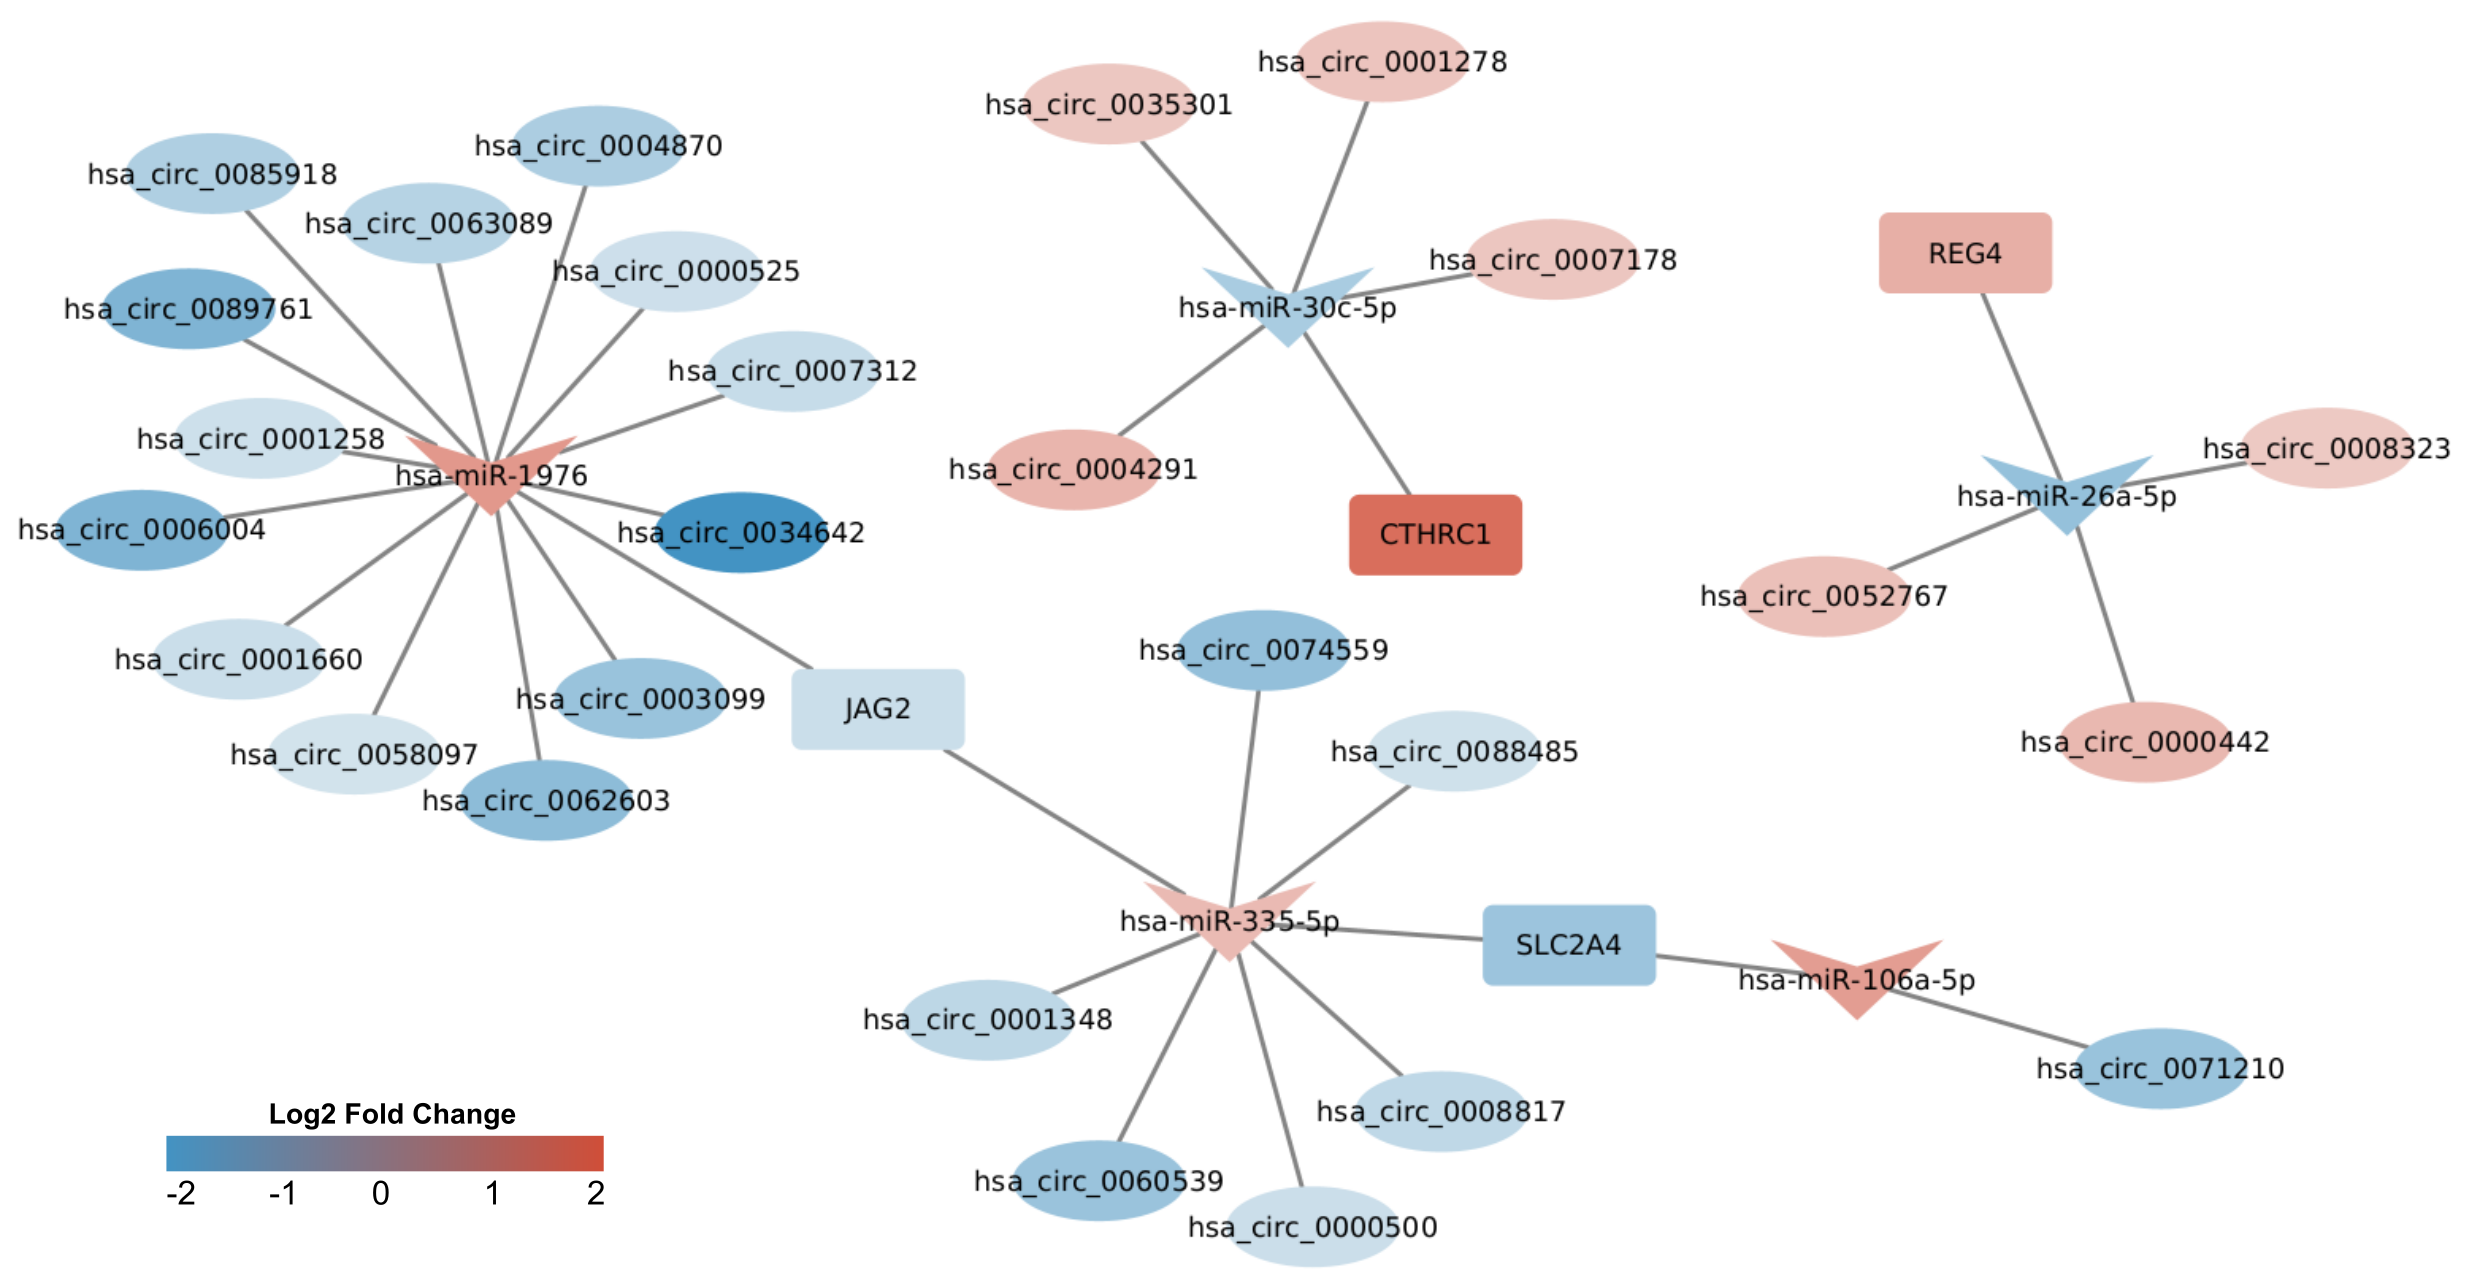
\includegraphics[width=\textwidth]{Chapter1/Figures/Figure3.png}
        \caption[Cytoscape visualisation of a ceRNA network]{\textbf{Cytoscape visualisation of a ceRNA network}. CircRNAs are represented as ellipse nodes, miRNAs as arrow nodes and mRNAs as rectangular nodes. Edges represent interactions predicted by both miRanda and TargetScan. The network has been filtered to select circRNA-miRNA-mRNA subgraphs representing circRNA sponging of miRNAs whereby upregulation of one biotype influences the expression of downstream targets.}
        \label{network}
    \end{center}
\end{figure}

\subsubsection{circRNA-RBP prediction}
Whilst circRNA-miRNA binding is the most studied functionality of circRNAs, there is increasing evidence to suggest circRNAs interact with multiple RBPs during their life cycle. Quaking (QKI), FUS, HNRNPL, RBM20 and Muscleblind are all RBPs which bind to specific intronic motifs, promoting the formation of circRNAs \cite{Ashwal-Fluss2014Oct, Conn2015Mar, Errichelli2017Mar, Fei2017Jun, Khan2016Oct}, whilst ADAR1 and DHX9 have been shown to destabilize inverted Alu repeats, supressing back-splicing \cite{Ivanov2015Jan, Aktas2017Apr}. \textit{CircPABPN1} has been shown to modulate the transcription of its cognate mRNA \textit{PABPN1} by competitively binding and reducing the availability of HuR, a translational activator protein \cite{Abdelmohsen2017Feb}. Additionally, \textit{circFoxo3} binds p21 and CDK2 RBPs, forming ternary complexes inhibiting cyclin E/CDK2 complex formation, arresting cells in G1 phase \cite{Du2016Apr}. \par
circRNA-RBP interactions can be characterised using cross-linking and immunoprecipitation (CLIP-seq) datasets however, the assay suffers from limitations. Firstly, CLIP-Seq reads are produced via enzymatic degredation, producing single-end reads of length $<$50bp. These short, single-end reads are unsuitable for traditional circRNA identification tools developed for RNA-Seq data which suffer from poor mapping estimates when using short reads and in the absence of paired-end reads, will generate high rates of false-positives. To accurately identify circRNAs in CLIP-Seq data, researchers can use Clirc, a computational tool capable of detecting BSJ sites bound to RBPs \cite{Clirc}. Clirc collapses reads to remove PCR duplicates prior to constructing a psuedo-reference based on publicly available human, mouse and drosophila circRNAs and circRNAs detected in ENCODE datasets using CIRI2. Reads that contiguously align to the reference genome are discarded, whilst reads mapping to the pseudo-reference are indicative of BSJ sites in circRNAs. The authors concede that Clirc is constrained to detecting circRNAs in the pseudo-reference and cannot detect circRNAs \textit{de novo}. Additionally, Clirc can only detect RBPs that directly bind to the BSJ site as distinguishing RBPs binding to `linear' sequences in circRNAs/mRNAs remains intractable. \par
Databases such as CircInteractome \cite{circinteractome} and starBase \cite{starbase} host results of circRNA-RBP interactions validated using CLIP-Seq experimental data. Due to the costs associated with CLIP-seq, there have been several computational methods developed to predict circRNA-RBP interactions by analysing motif sequences. CircRNAs Interact with Proteins (CRIP) is tool that represents circRNA-RBP interactions as a binary classification problem. The authors have developed a novel sequence encoding scheme whereby RNA triplets are represented as pseudo-amino acids, one-hot encoded and passed to a convolutional neural network (CNN) and a bidirectional long- and short-term memory (LSTM) network to exploit sequence information of 37 RBPs and the corresponding 32,216 circRNAs they bind \cite{CRIP}. Source code and training data are freely available, allowing users to leverage the information provided by CircInteractome to predict circRNA-RBP interactions using their own circRNA sequence data. This does however, require a high degree of computational competency to run, in which case users may find CirRBP \cite{CirRBP} a more suitable alternative. CirRBP utilizes a stacked ensemble deep learning model to predict RBP binding sites within a user supplied circRNA sequence, sourcing circRNA-RBP binding information from CircInteractome, starBase and CSCD2. The authors have packaged the underlying algorithm and models used for CirRBP as a publicly available webserver \cite{cirRBP-website} greatly reducing the computational barrier to entry for researchers to perform circRNA-RBP predictions. 


\subsection{circRNA databases}
Multiple circRNA databases currently exist providing users with circRNA annotations, predicted interactions, mature spliced sequence and expression estimates across cell lines (Table \ref{circdb}). Typically, these databases are derived from a selection of published ribosomal depleted RNA-Seq datasets \cite{findcirc,Salzman2012,Jeck2012Dec,Salzman2014Jun,Ivanov2015Jan,Rybak-Wolf2015Jun,Ashwal-Fluss2014Oct,Maass2017Nov} and are processed using a circRNA identification pipeline. It is worth noting that there is no universal `gold standard' pipeline for circRNA identification, thus each database will vary in their results. For example, circBase \cite{circbase} and CIRCpedia exclusively use find\_circ and CIRCexplorer2, respectively, whilst CSCD2 \cite{CSCD2} employs CIRI2, CIRCexplorer2, circRNA\_finder and find\_circ to produce its database, allowing users to identify which circRNAs have been called by multiple tools. Other databases such as circRNADb \cite{circrnadb} host circRNA annotations collated from published literature, removing biases inherent to specific pipelines. With respect to the functional interactions of circRNAs, the starBase \cite{starbase} and TRCirc \cite{TRCirc} databases contain RNA-RNA interactions and RNA-protein interactions using CLIP-Seq and CHIP-Seq data, respectively. Researchers can also search disease specific circRNAs backed by experimental findings in published literature via Circ2Disease \cite{circ2disease}. \par
One of the key challenges facing researchers when using circRNA databases is the lack of a standardised naming format for circRNAs. Chen et al. (2023) \cite{Chen2023Jan} use the example of the functional \textit{FAM20A} circRNA to depict the wide discrepancies between nomenclature: HSA\_CIRCpedia\_64725 in CIRCpedia, hsa-FAM120A\_0006 in circAtlas, hsa\_circFAM120A\_007 in circBank, and hsa\_circ\_0001875 in circBase. With `hsa' being the only common string between the four identifiers, Chen et al. proposed a novel naming convention for circRNAs. They provide examples for classic exonic circRNAs, EIcircRNAs and ciRNAs: 1) \textit{circCOX5A(2,3)} an exonic circRNA derived from the \textit{COX5A} gene that uses exons 2 and 3; 2) \textit{circCAMSAP1(2,RI,3)} an exonic-intronic circRNA derived from the \textit{CAMSAP1} gene that uses exons 2 and 3, with a retained intron (RI) between exons 2 and 3; 3) \textit{ciANKRD52(2)} an intronic circRNA derived from the \textit{ANKRD52} gene that retains the second intron. CircAtlas (version 3.0) \cite{circatlas3} provides users with mapping keys between circRNA positional, circBank, circBase and CIRCpedia identifiers to the latest 'uniform ID' values suggested by Chen et al. (2023). Whilst we agree that the standardisation of circRNA identifiers is a useful endeavour, we believe it may take several years to adopt. The main hurdle we observe is that the most popular circRNA identification tools that are currently in use by researchers are solely based on identifying BSJ reads in RNA-Seq data. These tools cannot fully resolve the internal structure of circRNAs, thus researchers are not able to accurately annotate internal exon/intron usage required to conform to the proposed naming convention. Secondly, circBase, CSCD2 and CIRCpedia remain hugely popular databases for circRNAs. Finally, the research community must agree on the reference used for reporting circRNAs (e.g ENSEMBL \cite{ENSEMBL2023}, RefSeq \cite{RefSeq}) and make clear which reference annotation files were used for circRNA annotation in order to make results reproducible.



\captionsetup[table]{labelfont=bf}
\begin{adjustwidth}{-1cm}{-1cm}
    \footnotesize
    \begin{longtblr}[
        entry = {Publicly available online circRNA databases},
        caption = {\textbf{Publicly available online circRNA databases}.},
        label = {circdb},
        note{1} = {Species abbreviations: ade, \textit{Actinidia deliciosa}; ath, \textit{Arabidopsis thaliana}; bdi, \textit{Brachypodium distachyon}; bta, \textit{Bos taurus}; cel, \textit{Caenorhabditis elegans}; csi, \textit{Camellia sinensis}; dme, \textit{Drosophila melanogaster}; dre, \textit{Danio rerio}; gar, \textit{Gossypium arboreum}; gga, \textit{Gallus gallus}; ghi, \textit{Gossypium hirsutum}; gma, \textit{Glycine max}; gra, \textit{Gossypium raimondii}; gsp, \textit{Gossypium spp.}; hsa, \textit{Homo sapiens}; hvu, \textit{Hordeum vulgare}; lch, \textit{Latimeria chalumnae}; lme, \textit{Latimeria menadoensis}; mml, \textit{Macaca mulatta}; mmu, \textit{Mus musculus}; nbe, \textit{Nicotiana benthamiana}; ocu, \textit{Oryctolagus cuniculus}; osa, \textit{Oryza sativa}; osi, \textit{Oryza sativa ssp. indica}; pbe, \textit{Pyrus betulifolia}; ptr, \textit{Poncirus trifoliata}; rno, \textit{Rattus norvegicus}; sly, \textit{Solanum lycopersicum}; ssc, \textit{Sus scrofa}; stu, \textit{Solanum tuberosum}; sly, \textit{Solanum lycopersicum}; tae, \textit{Triticum aestivum}; zma, \textit{Zea mays}},
        note{\textsuperscript{*}} = {URL not accessible at time of drafting review}
        ]{
        colspec = {lX[5]Xr} %% put weights for column width in [] 
        }
        \hline
        \textbf{Database} & \textbf{Data available} & \textbf{Organisms}\textsuperscript{1} & \textbf{Reference} \\
        \hline
        \href{https://deepbiology.cn/circRNA/}{AtCircDB} & A. thaliana circRNAs, miRNA targets & ath &  \cite{atcircdb} \\
        \href{https://ngdc.cncb.ac.cn/circatlas/}{circAtlas} & circRNA sequences, conservation score, miRNA \& RBP targets, isoforms, expression in tissues, junction ratio, reported diseases & hsa, mml, mmu, rno, ocu, clf, fca, ssc, oar, gga & \cite{circatlas} \\        
        \href{http://www.circbase.org/}{circBase} & circRNA sequences, circRNA expression in cell lines/tissues & hsa, mmu, cel, lch, lme & \cite{circbase} \\
        \href{http://www.circbank.cn/}{CircBank}\textsuperscript{*} & miRNA targets, m\textsuperscript{6}A modifications, conservation, mutations and coding potential & hg19 & \cite{circbank} \\
        \href{https://circinteractome.nia.nih.gov/}{CircInteractome} & miRNA \& RBP targets, primer design, siRNA sites & hsa & \cite{circinteractome} \\
        \href{https://awi.cuhk.edu.cn/~CircNet/php/index.php}{CircNet} & miRNA \& RBP targets, ceRNA networks construction, coding potential & hsa & \cite{circnet} \\
        \href{https://bis.zju.edu.cn/CircFunBase/index.php}{CircFunBase} & circRNA predicted function, miRNA \& RBP targets, visual representation of ceRNA network & ath, osa, tae, sly, gsp, hvu, ade, hsa, mml, rno, mmu, gga, ssc, bta, dme, ocu & \cite{circfunbase} \\
        \href{http://yang-laboratory.com/circpedia}{CIRCpedia} & circRNA exprression in cells and tissues & hsa, mmu, cel, dme, dre, rno & \cite{circpedia} \\
        \href{http://gb.whu.edu.cn/CSCD2/}{CSCD2} & circRNAs in cancer, target miRNAs \& RBP, coding potential & hsa & \cite{CSCD2} \\
        \href{http://reprod.njmu.edu.cn/cgi-bin/circrnadb/circRNADb.php}{circRNADb} & exonic circRNAs, coding potential & hsa & \cite{circrnadb} \\
        \href{https://hanlab.uth.edu/cRic/}{CircRiC}\textsuperscript{*} & circRNAs in cancer & hsa & \cite{CircRiC} \\
        \href{http://bioinformatics.zju.edu.cn/Circ2Disease/}{Circ2Disease} & circRNAs associated with diseases & hsa & \cite{circ2disease} \\
        \href{http://bioinfo.snnu.edu.cn/CircR2Disease/}{CircR2Disease} & circRNAs associated with diseases & hsa & \cite{circr2disease} \\
        \href{http://gyanxet-beta.com/circdb/}{Circ2Traits}\textsuperscript{*} & circRNA-miRNA disease associations & hsa & \cite{circ2traits} \\
        \href{http://cgga.org.cn:9091/circRNADisease/}{circRNADisease}\textsuperscript{*} & circRNAs associated with diseases & hsa & \cite{circrnadisease} \\
        \href{http://deepbiology.cn/crop/}{CropCircDB} & circRNAs in maize \& rice & osa, zma & \cite{cropcircdb} \\
        \href{https://rna.sysu.edu.cn/deepbase3/}{DeepBase} & circRNA, lncRNA, miRNAs in tissues and cancers & hsa & \cite{deepbase} \\
        \href{http://www.exorbase.org/}{exoRBase} & Atlas of mRNAs, lncRNAs,\& circRNAs in extracellular vesicles & hsa & \cite{exoRBase} \\
        \href{https://mioncocirc.github.io/}{MiOncoCirc} & Compendium of circRNA datasets in cancer & hsa & \cite{mioncocirc} \\
        \href{https://voineagulab.github.io/NeuroCirc/}{NeuroCirc} & circRNA expression in brain regions, circQTLs & hsa & \cite{neurocirc} \\
        \href{https://bis.zju.edu.cn/plantcircnet/index.php}{PlantCircNet}\textsuperscript{*} & ceRNA regulatory networks & ath, gma, hvu, osa, sly, tae, zma, bdi & \cite{plantcircnet} \\
        \href{http://ibi.zju.edu.cn/plantcircbase/}{PlantcircBase} & circRNAs in plants, ceRNA regulatory network & ath, gma, hvu, osa, sly, tae, zma, gar, ghi, gra, ptr, stu, csi, nbe, pbe, osi & \cite{plantcircbase} \\
        \href{https://rnasysu.com/encori/}{starBase} & RNA-RNA interactions based on CLIP-Seq data & 23 species & \cite{starbase} \\
        \href{https://bio.liclab.net/TRCirc/view/index}{TRCirc} & Transcriptional regulation of circRNAs using CHIP-Seq data & hsa & \cite{TRCirc} \\
        \hline
    \end{longtblr}
\end{adjustwidth}

\subsection{Concluding remarks}
circRNAs are a class of non-coding RNAs which are gaining recognition for their roles in cellular processes as transcriptional regulators. Despite circRNAs representing an increasingly popular area of research, there still remain several challenges in accurately characterising circRNAs computationally. This is perhaps most apparent in a subset of widely utilised circRNA identification tools that are entirely predicated on detecting the BSJ of circRNAs in sequencing data. Whilst these tools are useful for detecting and quantifying circRNAs, they struggle to fully resolve the full circRNA sequence or delineate circRNA isoforms generated from the same BSJ. Furthermore, these tools suffer from varying rates of sensitivity and depending on the underlying methods used, can be prone to false positives. Integrated methods have been developed to address this issue however, these tools can hardly be considered a panacea given recent studies have shown circRNAs called by multiple tools can fail external validation. The development of a gold standard set of circRNAs is a necessary step to benchmark the performance of current and future circRNA identification tools, diagnosing their inherent blind spots. Another striking absence in the field of circRNA research is the lack of a reference GTF/GFF file of known circRNAs. In our opinion this goes hand in hand with the development of a gold standard set of circRNAs and the unification of circRNA nomenclature. Once developed, the research community can report circRNAs in a consitent manner and develop rapid pseudo-alignment based tools mimicking those in the space of RNA-Seq (Kallisto\cite{kallisto}, Salmon\cite{Salmon}). Third-generation sequencing represents a promising avenue for full circle characterisation of circRNAs and accurate prediction of interactions with miRNAs and RBPs. However, few computational tools consider the final tertiary structure of circRNAs which can greatly influence its capacity to bind miRNAs and RBPs or form scaffold structures. \par
In conclusion, our work provides an accessible guide for researchers to navigate the landscape of computational circRNA research. We have provided a comprehensive overview of the tools available for circRNA identification, full circle reconstruction, differential expression analysis, circRNA interactions and databases, highlighting the limitations of current tools and suggesting solutions to common pitfalls. \par
In the next chapter, we detail the development and benchmarking of nf-core/circrna, our own solution for integration-based circRNA identification. nf-core/circrna takes as input raw RNA-Seq data and automatically downloads reference genome and annotations files, with support for up to 18 species. Users can avail of up to 7 circRNA quantification tools coupled with robust filtering methods to obtain high confidence circRNAs for downstream miRNA target prediction and differential expression analysis. Developed using nextflow and incorporated within the nf-core suite of gold-standard pipelines, nf-core/circrna comes with comprehensive documentation and an active research community driving continuous refinement and development of workflows. 
{\Huge \bfseries \noindent Chapter 3}
\vspace{-1em} 
\section*{\LARGE nf-core/circrna: a portable workflow for the quantification, miRNA target prediction and differential expression analysis of circular RNAs}
\addcontentsline{toc}{section}{3\quad nf-core/circrna: a portable workflow for the quantification, miRNA target prediction and differential expression analysis of circular RNAs}
\setcounter{section}{3}
\setcounter{subsection}{0}  % reset so next \subsection is 2.1
\renewcommand{\chapternum}{3}

% Reset figure/table numbering per chapter
\renewcommand{\thefigure}{\chapternum.\arabic{figure}}
\setcounter{figure}{0}
\renewcommand{\thetable}{\chapternum.\arabic{table}}
\setcounter{table}{0}


\begin{center}
    \textit{The content of this chapter has been published as:} \par
    \vspace{0.55cm}
    \textbf{Barry Digby}, Stephen P. Finn, and Pilib Ó Broin. “nf-core/circrna: a portable
workflow for the quantification, miRNA target prediction and differential ex-
pression analysis of circular RNAs”. In: BMC Bioinf. 24.1 (Dec. 2023), pp. 1-15.
ISSN: 1471-2105. DOI: 10.1186/s12859-022-05125-8.
\end{center}

\subsection*{Abstract}

Circular RNAs (circRNAs) are a class of covalently closed non-coding RNAs that have garnered increased attention from the research community due to their stability, tissue-specific expression and role as transcriptional modulators via sequestration of miRNAs. Currently, multiple quantification tools capable of detecting circRNAs exist, yet none delineate circRNA-miRNA interactions, and only one employs differential expression analysis. Efforts have been made to bridge this gap by way of circRNA workflows, however these workflows are limited by both the types of analyses available and computational skills required to run them.


We present nf-core/circrna, a multi-functional, automated high-throughput pipeline implemented in nextflow that allows users to characterise the role of circRNAs in RNA Sequencing datasets via three analysis modules: (1) circRNA quantification, robust filtering and annotation (2) miRNA target prediction of the mature spliced sequence and (3) differential expression analysis. nf-core/circrna has been developed within the nf-core framework, ensuring robust portability across computing environments via containerisation, parallel deployment on cluster/cloud-based infrastructures, comprehensive documentation and maintenance support. nf-core/circrna reduces the barrier to entry for researchers by providing an easy-to-use, platform-independent and scalable workflow for circRNA analyses. Source code, documentation and installation instructions are freely available at \href{https://nf-co.re/circrna}{https://nf-co.re/circrna} and \href{https://github.com/nf-core/circrna}{https://github.com/nf-core/circrna}.


\subsection{Introduction}

CircRNAs are a class of non-coding RNAs (ncRNAs) formed by the back-splicing of precursor messenger RNA (pre-mRNA) to create a single-stranded covalently closed RNA loop structure. Initially discovered in plant viroids \cite{Sanger1976}, yeast mitochondrial RNAs \cite{Arnberg1980Feb}, and the hepatitis $\delta$ virus \cite{Kos1986Oct}, circRNAs were believed to be a by-product of aberrant splicing or intermediates discarded from intron-lariat debranching \cite{Cocquerelle1993Jan,Qian1992}, going largely unstudied during the formative years of RNA-Seq due to poly-A selection protocols. Recent advancements in bioinformatics methods have facilitated the detection of circRNAs in RNA-Seq datasets, with interest in the field revitalised when Salzman et al. identified circRNAs in cancer and non-cancer cell lines \cite{Salzman2012} resulting in a shift in the paradigm of RNA-Seq protocols enabling detection of circRNAs (total RNA-Seq, ribosomal RNA (rRNA) depleted RNA-Seq). \par
Several characteristics of circRNAs make them ideal candidates as clinical biomarkers for cancers and diseases; lack of 5' and 3' ends conferring resistance to RNase degradation granting much higher half-lives than their linear counterparts \cite{Salzman2012,findcirc}, tissue- and developmental-stage specific expression, and abundance in blood, serum, plasma and exosomes \cite{Memczak2015, Bahn2015}. Recent evidence has accumulated demonstrating circRNAs viability as a biomarker, with reports of circRNAs exhibiting differential expression in gastric cancer \cite{Li2015Apr}, colorectal cancer \cite{Bachmayr-Heyda2015}, bladder cancer \cite{Zhong2016}, cardiovascular disease \cite{Tan2016} and Alzheimer's disease \cite{Panda2017} amongst many others. circRNAs have also been shown to harbour functionally active and evolutionarily conserved microRNA response elements (MREs) within their mature spliced sequence \cite{Hansen2013Mar,Thomas2014Aug}, suggesting a regulatory role within the competing endogenous RNA (ceRNA) network by titrating the limited pool of endogenous miRNAs available to mRNAs \cite{Denzler2014Jun}. One such example is circCCDC66, which is hypothesized to play a protective role for the MYC oncogene by binding to miR-33b and miR-99 in colorectal cancer. Knockdown of circCCDC66 displayed reduced MYC expression, whilst administration of miR-33b and miR-99 reversed the knockdown effect, inferring circCCDC66 is capable of modulating mediating MYC expression via the ceRNA network \cite{Hsiao2017}.
\par
Regarding the quantification, miRNA target prediction and differential expression analysis of circRNAs, several workflows currently exist (Table \ref{tab:c2workflowtables}). However, the majority of these workflows are limited by the type of analysis they can perform, often acting as either: 1) a downstream analysis toolkit requiring the user to supply circRNA quantification results, or 2) a workflow offering multiple quantification tools to generate high confidence circRNA calls. Both scenarios necessitate in-house computational expertise to supplement the missing elements of the analysis, resulting in a high barrier to use for both novice and seasoned researchers alike due to the non-standardised input requirements to each workflow.\par


\begin{centering}
\begin{table}[h!]
    \caption[List of current circRNA analysis workflows]{\textbf{List of current circRNA analysis workflows}.}
    \resizebox{\textwidth}{!}{%
    \begin{tabular}{lllcccc}
    \toprule
    \textbf{Pipeline} & \textbf{Published} & \textbf{Dependencies} & \textbf{CQ} & \textbf{MP} & \textbf{DE} & \textbf{Installation} \\ \toprule 
    CirComPara \cite{CirComPara} & 2017 & \begin{tabular}[c]{@{}c@{}}Python, R\\ or Docker\end{tabular} & \cmark & \xmark & \begin{tabular}[c]{@{}l@{}}linear\\ RNA\end{tabular} & \begin{tabular}[c]{@{}c@{}}Source code,\\ DockerHub\end{tabular} \\
    CirComPara2 \cite{CirComPara2} & 2021 & \begin{tabular}[c]{@{}l@{}}Python, R\\ or Docker\end{tabular} & \cmark & \xmark & \xmark & \begin{tabular}[c]{@{}c@{}}Source code,\\ DockerHub\end{tabular} \\
    DEBKS \cite{DEBKS} & 2021 & Python & \xmark & \xmark & \cmark & \begin{tabular}[c]{@{}c@{}}Source code,\\ Conda, pip\end{tabular} \\
    FcircSec \cite{FcircSEC} & 2020 & R & \xmark & \xmark & \xmark & CRAN \\
    circRNAProfiler \cite{circRNAprofiler} & 2020 & R & \xmark & \cmark & \cmark & Bioconductor \\
    circtools \cite{circtools} & 2019 & Python, R & \cmark & \xmark & \cmark & Conda, Pypi \\
    circMeta \cite{circmeta} & 2020 & R & \xmark & \xmark & \cmark & \begin{tabular}[c]{@{}c@{}}Source code\\ via devtools\end{tabular} \\
    circRNAwrap \cite{circRNAwrap} & 2019 & Perl, Python, R & \cmark & \xmark & \cmark & \begin{tabular}[c]{@{}c@{}}Manual\\ Installation\end{tabular} \\
    Ularcirc \cite{Ularcirc} & 2019 & R, R Shiny & \xmark & \cmark & \xmark & Bioconductor \\
    \textbf{nf-core/circrna} \cite{Digby2023Dec} & \textbf{2023} & \textbf{\begin{tabular}[c]{@{}c@{}}nextflow, java,\\ Docker/Apptainer\end{tabular}} & \textbf{\cmark} & \textbf{\cmark} & \textbf{\cmark} & \textbf{DockerHub} \\ \toprule
    \multicolumn{7}{l}{\begin{tabular}[c]{@{}l@{}}\textbf{\textit{CQ}} circRNA quantification\\ \textbf{\textit{MP}} miRNA prediction\\ \textbf{\textit{DE}} differential expression\end{tabular}}
    \end{tabular}}
\label{tab:c2workflowtables}
\end{table}
\end{centering}

To address these shortcomings, we present nf-core/circrna, a workflow for the quantification, miRNA target prediction and differential expression analysis of circRNAs in RNA-Seq data developed using nextflow \cite{DiTommaso2017}. The pipeline has been developed under the specifications of the nf-core framework \cite{Ewels2020Mar}, ensuring best practices in pipeline development and maintenance.

\subsection{Implementation}
\subsubsection{nf-core/circrna architecture}
The workflow is modularised via processes, whereby each process represents an individual task within the workflow. Nextflow automatically distributes each process in an isolated environment where task execution is performed within a container, ensuring efficient utilization and scaling of computing resources user-defined via configuration files. By utilising containers, the arduous task of installing and satisfying software dependencies has been completely removed, thereby facilitating rapid `out of the box' deployment and ensuring reproducible analyses through pinned software versions.
\par
nf-core/circrna is configured to run on local machines, high performance compute clusters and cloud infrastructures alike, facilitating most deployment scenarios via customisable configuration profiles. Profiles for popular platforms (AWS, Azure, Google Cloud) and multiple research institutions can be found at (\url{https://github.com/nf-core/configs}). In the event ones institution is not represented, users are encouraged to fork the nf-core/circrna repository and make the appropriate changes to the configuration profile, reflecting the task scheduler and min/max computational resources available before attempting to deploy the workflow.
\par
Comprehensive documentation including instructions to perform a test dataset analysis can be found at \url{https://nf-co.re/circrna}. Furthermore, the nf-core community harbours an active Slack channel where users can contact the authors directly with queries regarding the workflow, or open an issue on the workflows github page. Three dependencies are required to run nf-core/circrna: Java ($>$=8), the latest version of nextflow \cite{DiTommaso2017} and a software container client such as Docker \cite{Docker} or Apptainer (formerly Singularity) \cite{Apptainer}.

\subsubsection{nf-core/circrna functionality}
The functionality of nf-core/circrna can be summarized by three core analysis modules: 1) circRNA discovery and quantification 2) miRNA target prediction and 3) differential expression analysis (Figure \ref{fig:1}). The circRNA discovery module is required, however users may choose to include or omit the miRNA prediction or differential expression modules to suit their analysis needs. Pre-processing steps are optional, depending on the format and quality of the input data supplied to the workflow.
\par
The pipeline accepts paired-end RNA-Seq data in the form of FASTQ files or BAM files as inputs to the workflow. In the event BAM files are supplied, the workflow will automatically revert the BAM files to paired end FASTQ files for back-splice junction detection. Summary statistics of read quality, sequencing artefacts and adapter contamination are generated using FastQC \cite{Andrews}, with an optional parameter available to perform adapter removal and read filtering using BBDUK \cite{Bushnell}, allowing the user to pass raw or trimmed reads to the circRNA discovery module. 
\par
Reference annotation files (FASTA, GTF) are automatically downloaded via the Illumina iGenomes database, with 18 species currently supported by the workflow in ENSEMBL, UCSC and NCBI annotations where available. In addition to providing correctly formatted reference files to the workflow, the iGenomes database hosts genome index files compatible with multiple aligners, significantly reducing the computational cost of analyses. In the event the user is working with a non-model organism, reference files can be supplied to the workflow manually.

\begin{figure}[h!]
    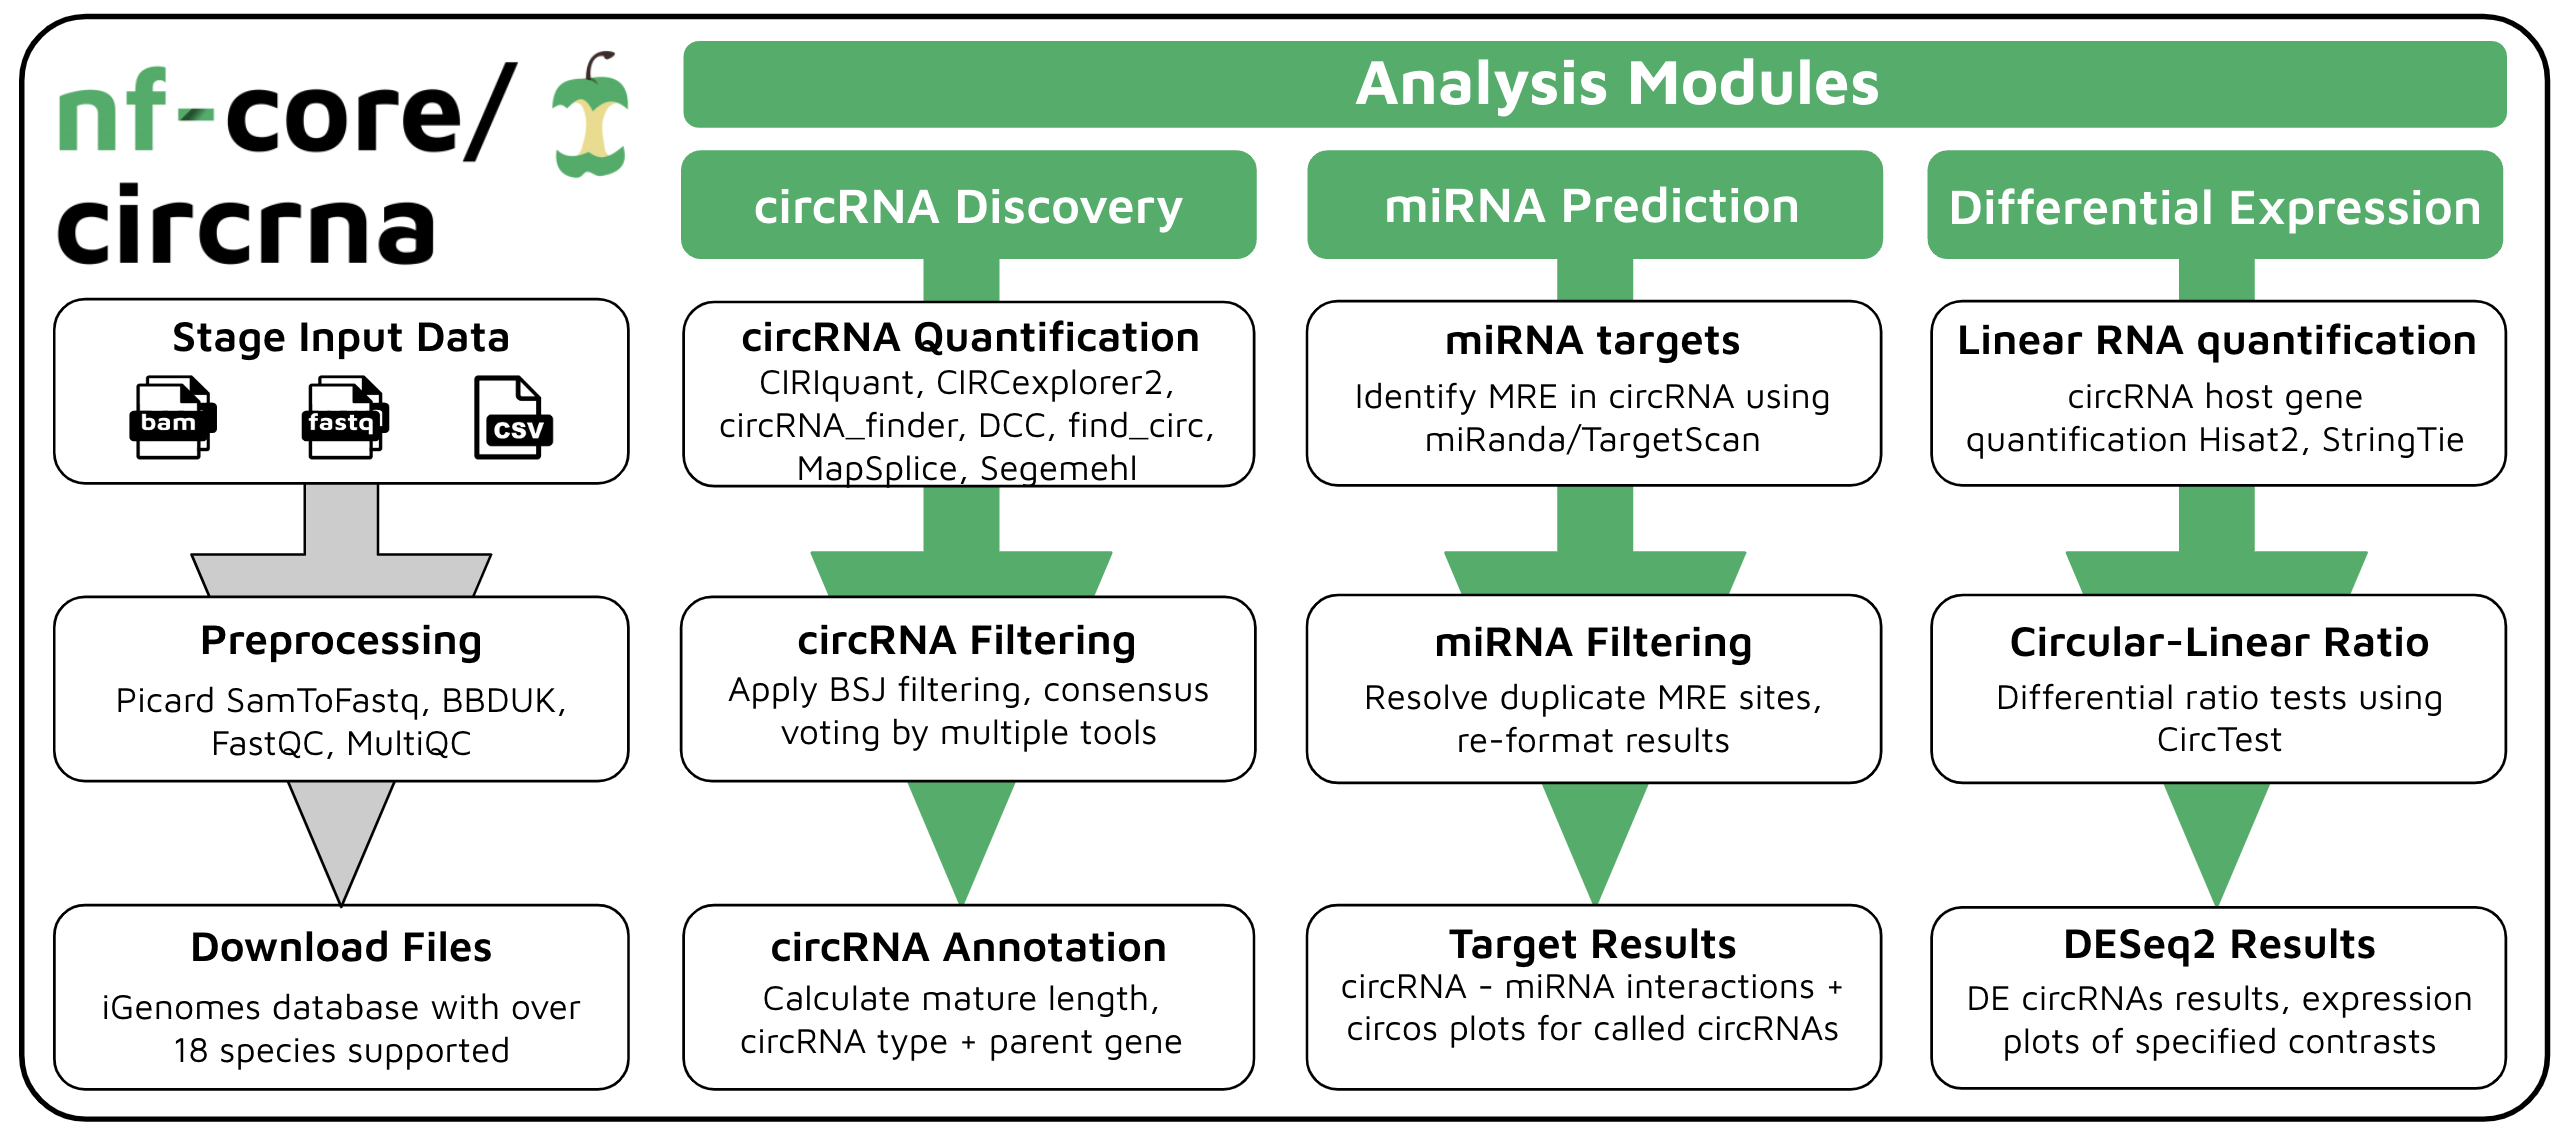
\includegraphics[width=\textwidth]{Chapter2/Figures/figure1.png}
    \vspace{-5mm}
    \caption[Schematic overview of nf-core/circrna analysis modules]{\textbf{Schematic overview of nf-core/circrna analysis modules}.}
    \label{fig:1}
\end{figure}

\subsubsection{circRNA Discovery}
nf-core/circrna currently offers seven circRNA quantification tools: CircExplorer2 \cite{CIRCexplorer2}, circRNA\_finder \cite{circRNAfinder}, DCC \cite{DCC}, CIRIquant \cite{CIRIquant}, MapSplice \cite{MapSplice}, find\_circ \cite{findcirc} and Segemehl \cite{segemehl}. As both CIRCexplorer2 and CIRIquant can parse the outputs from multiple aligners, we define CIRCexplorer2 as utilising STAR \cite{STAR} 2-pass mode prior to parsing, whilst CIRIquant utlises its canonical BWA \cite{BWA} - CIRI2 \cite{CIRI2} workflow. The user may select one, all or any combination of circRNA tools available in the workflow by providing a list to the `\code{-{}-tool}' parameter. In the scenario where more than one quantification tool has been selected, the parameter `\code{-{}-tool\_filter}' accepts as input a positive integer \textit{n} to perform consensus based filtering on called circRNAs, requiring circRNAs to be called by at least \textit{n} quantification tools during the count matrix generation step. Users can also apply one of two aggregation functions to circRNAs called by multiple tools using the `\code{-{}-}duplicates\_fun' parameter, which accepts `max' or `mean' returning the highest count value or averages, respectively. To reduce spurious circRNA candidates, the parameter `\code{-{}-bsj\_filter}' filters circRNAs based on the number of reads spanning the back-splice junction site during parsing of the raw quantification tool outputs.
\par 
Candidates that satisfy the filtering thresholds are passed to an in-house reference-guided circRNA annotation script detailing circRNA type, parent gene, underlying exons and mature spliced length, producing an extended BED-12 output file. The in-house script considers the four following cases for circular candidates: \textit{Circular candidates start and end positions overlap exon boundaries}: If circular candidates start and end positions perfectly overlap exon boundaries, the
candidate is marked as an exonic circRNA, or simply `circRNA'. \textit{Circular candidates start and end positions imperfectly overlap exon boundaries}: If the start and end positions are suitably within range ($<$ 200bp) of an exon boundary, the candidate is assumed to be a circRNA. However, if one of the start or end position reside outside of the range of an exon boundary ($>$ 200bp), the circular candidate is assumed to be an exon-intron circRNA (EI-circRNA). Users can toggle the 200bp distance via the `\code{-{}-exon\_boundary}' parameter. \textit{Circular candidate resides within a gene, but does not overlap any exon boundaries}: These circular candidates are marked as intronic circular RNAs (ciRNAs). \textit{Circular candidates do not overlap any features in the reference GTF file}: Such candidates are assumed to be intergenic circRNAs and will have an `NA' description for underlying transcripts and parent gene in the output file. Due to the scripts reliance on reference annotations, the workflow is suitable only for analyses of species for which a reference GTF file exists.
\par
Finally, utilising the information held in the BED12 file, the circRNA\_discovery module outputs the mature spliced sequence of each called circRNA in FASTA format and generates a circRNA count matrix for downstream statistical testing, which are used as inputs for the `miRNA\_prediction' and `differential\_expression' modules, respectively. To access the raw output files generated by each quantification tool, users can toggle the `\code{-{}-save\_intermediates} boolean parameter to copy files from the work directory to the specified results directory.
\par

\subsubsection{miRNA prediction}
To elucidate the regulatory role of circRNAs, nf-core/circrna offers a miRNA prediction module to identify miRNA response element (MRE) sites within the mature spliced sequence and back-splice junction site of detected circRNAs using both miRanda \cite{miranda} and TargetScan \cite{Targetscan} prediction algorithms. To reduce the number of spurious calls, target miRNAs must be called by both target prediction algorithms. The predictions are output in a results file per sample, detailing circRNA-miRNA node/edge membership complete with miRanda scores, minimum free energy (Kcal/mol) and site type (6mer, 7mer-m8, 7mer-A1, 8mer). Should the user wish to apply strict post-hoc filtering, we suggest users remove 6mers and miRNAs with a minimum free energy score of $>=$-20.00Kcal/Mol \cite{Clark2018}.

\subsubsection{Differential expression analysis}
nf-core/circrna offers a differential expression module to detect differentially expressed circRNAs and model changes in circRNA expression relative to its host gene guided by the phenotype.csv file provided by the user. It is important to note that pre-filtered datasets with linear RNAs removed are not suitable for the differential expression module. \par Firstly, linear RNAs are quantified using Hisat2 and StringTie \cite{Pertea2016} to determine both host gene expression and library size factors, which are utilised to normalize the circRNA count matrix. Following normalization, quality control plots are generated to assess sample heterogeneity: analysis of principal components via PCA plots and hierarchical clustering of samples via heatmaps and dendograms. The workflow automates differential expression analysis for all possible combinations of the levels provided under the column `condition', whilst controlling for additional covariates added to the phenotype design file using DESeq2 \cite{Love2014Dec}. For each contrast, the workflow reports both up-regulated and down-regulated circRNAs, plots of global expression patterns via heatmaps, volcano and MA plots, and the distribution of adjusted and non-adjusted p-values. Furthermore, for each differentially expressed circRNA returned by the contrast, boxplots are generated displaying the normalized expression between experimental conditions. To compliment the circRNA results, the workflow concurrently performs linear RNA-Seq differential expression analysis. \par
The CircTest \cite{DCC} R package employs a beta-binomial model to test differences between circRNA and host gene expression to identify cases of enrichment or depletion of circRNA relative to the linear transcripts from the same host genes. The module outputs PDF plots of circRNA-host gene line plots, ratio plots and a table of the statistical results for users.

\subsection{Results and discussion}
\subsection*{nf-core/circrna demonstration full dataset}
To showcase the utility of nf-core/circrna in a single execution, we recapitulated a previously published study investigating the effect of mutant RNA binding homolog FUST-1 on circRNA biogenesis in total RNA seq samples of \textit{C. elegans} (PRJNA742881) \cite{Cao2021} Table \ref{tab:celdataset}. \par

\begin{table}[h!]
\centering
\caption[Run information using PRJNA742881 dataset]{\textbf{Run information using PRJNA742881 dataset}}
\label{tab:celdataset}
\resizebox{\textwidth}{!}{%
\begin{tabular}{cccccc}
\toprule
\shortstack{\textbf{Project}\\\textbf{Accession}} & \shortstack{\textbf{Genome}\\\textbf{Build}} & \shortstack{\textbf{Run}\\\textbf{Time}} & \shortstack{\textbf{CPU}\\\textbf{Hours}} & \shortstack{\textbf{Sample}\\\textbf{ID}} & \shortstack{\textbf{Number of}\\\textbf{reads}} \\
\midrule
\multirow{6}{*}{PRJNA742881} & \multirow{6}{*}{WBcel235} & \multirow{6}{*}{18h 21m 20s} & \multirow{6}{*}{1566} & N2\_1 & 72651039 \\
    &   &   &   & N2\_2  & 92546415  \\
    &   &   &   & N2\_3  & 82870805   \\
    &   &   &   & fust1\_1 & 70194536 \\
    &   &   &   & fust1\_2 & 89945035 \\
    &   &   &   & fust1\_3 & 86470345  \\
\bottomrule
\end{tabular}%
}
\end{table}


Setting up the analysis required minimal effort -- raw sequencing data was retrieved using nf-core/fetchngs \cite{fetchngs} by providing the sequencing archive project accession number, a sample CSV file was constructed specifying the sample ID's and sample paths, a phenotype CSV file was designed detailing sample metadata for DESeq2 and both the `WBcel235' and `cel' strings were passed to the workflow to automatically download ENSEMBL reference annotation and miRNA database files, respectively. The analysis was run on a local SLURM HPC cluster with maximum ncpu and cpu memory limits set to 8 and 60 GB, representing a moderate level of resources feasible for most research labs. \par

\begin{figure}
    \makebox[\textwidth][c]{
    \includegraphics[width=1.2\textwidth]{Chapter2/Figures/figure2.png}
    }
    \vspace{5mm}
    \caption[Comparison of filtered PRJNA742881 circRNAs]{\textbf{Comparison of filtered circRNAs} \textbf{(A)} circRNAs called by each quantification tool in this study. \textbf{(B)} common circRNAs in this study vs. PRJNA742881. Filtered circRNAs were required to have at least 15 BSJ reads called by CIRIquant. \textbf{(C)} Genomic distribution of 4435 common filtered circRNAs (outer layer), 2420 additional circRNAs discovered by nf-core/circrna (middle layer) and 521 circRNAs unique to PRJNA742881 (inner layer).}
    \label{fig:2}
\end{figure}

\begin{centering}
\begin{figure}[h!]
    \makebox[\textwidth][c]{
    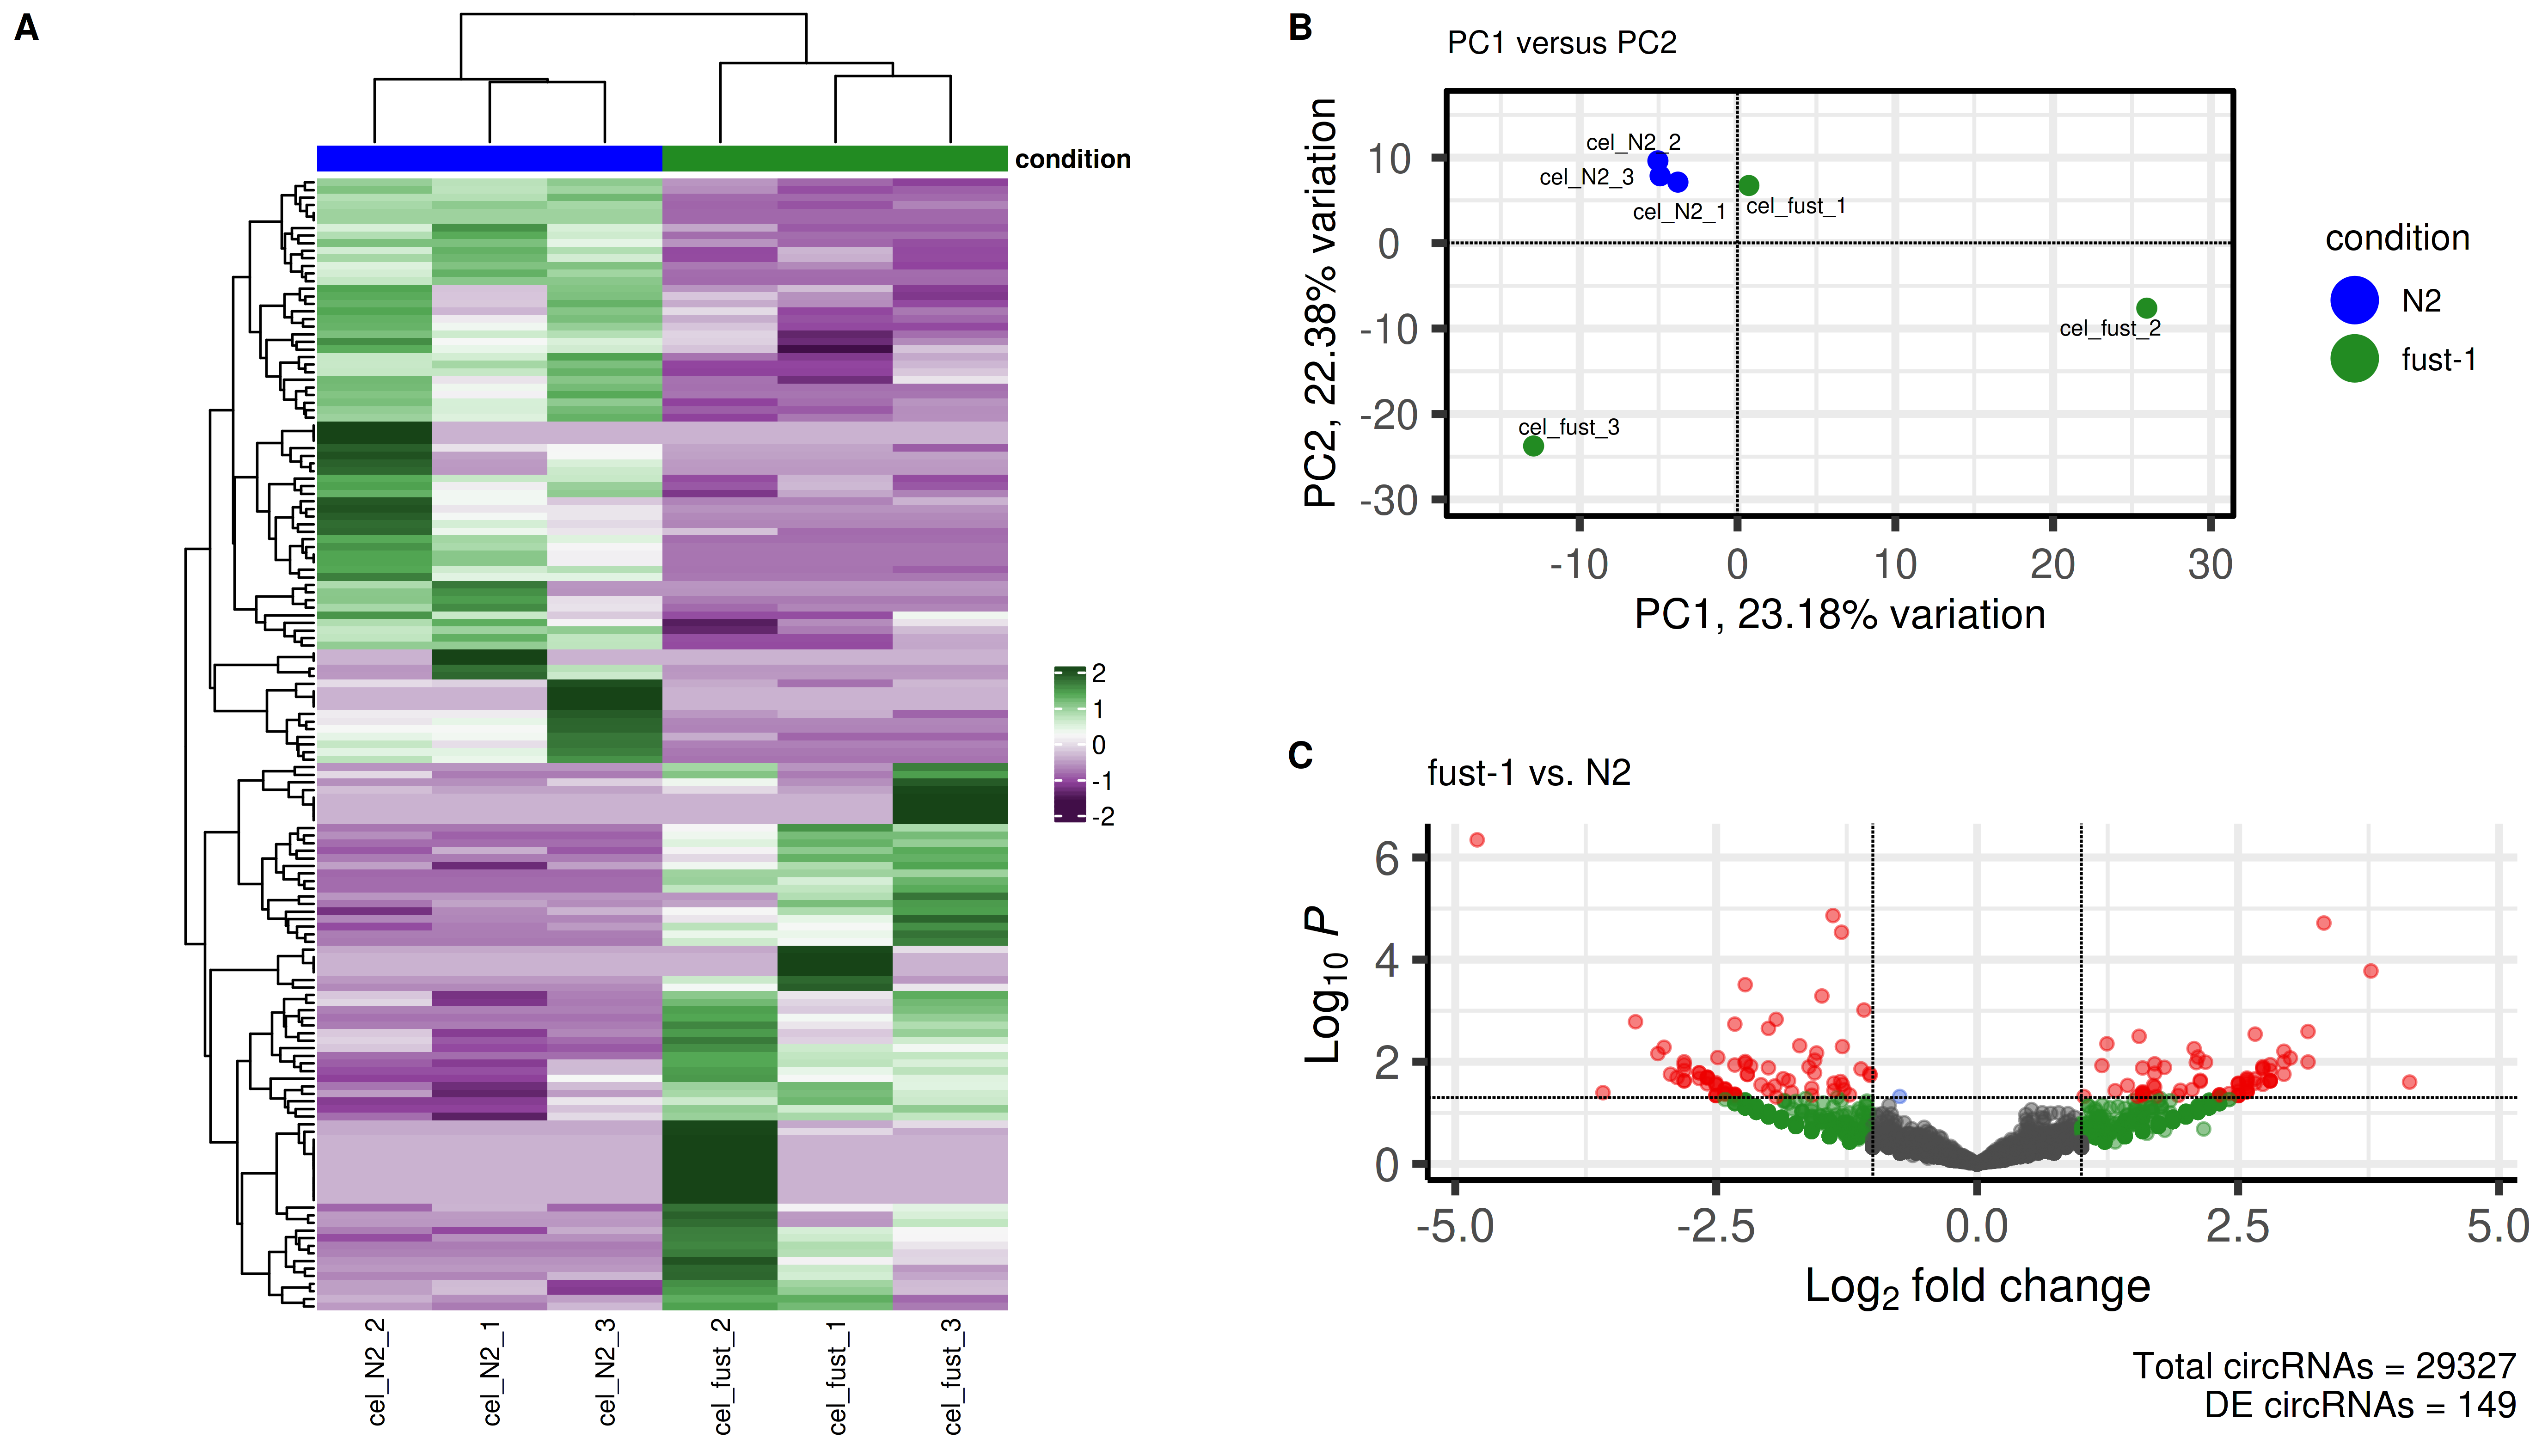
\includegraphics[width=1.2\textwidth]{Chapter2/Figures/figure3.png}
    }
    \vspace{5mm}
    \caption[Workflow outputs (PRJNA742881)]{\textbf{nf-core/circrna sample outputs (PRJNA742881)}: \textbf{(A)} Heatmap of differentially expressed circRNAs \textbf{(B)} Principal component bi-plot of PRJNA742881. \textbf{(C)} Volcano plot of differentially expressed circRNAs.}
    \label{fig:3}
\end{figure}
\end{centering}

Based on the results of the simulated dataset (Table \ref{tab:metrics}), CIRCexplorer2, CIRIquant, find\_circ and MapSplice were chosen for circRNA quantification due to their high F1 scores ($>$ 91\%). The original analysis by Cao et. al used CIRCexplorer2, DCC and CIRI2. The justification for not using CIRI2 and DCC are as follows: CIRIquant is the successor to CIRI2, acting as a wrapper script around CIRI2 and as such, CIRI2 remains the underlying circRNA detection software. DCC requires an extremely high amount of RAM (analysis failed with 120GB RAM allocated to DCC processes), most likely caused by the exceptionally high coverage of circRNAs in the RNase R Treatment, Polyadenylation, and Poly(A)$+$ RNA Depleted (RPAD) dataset. Due to it's computational inefficiency and high false positive rate in Table \ref{tab:metrics}, we reasoned that the analysis would not suffer due to its omission. \par
In less than 19 hours, a single execution of nf-core/circrna produced a comprehensive profile of circRNAs in N2 and fust1 \textit{C. elegans} samples, recovering 4,435 filtered circRNAs detected by Cao et al. and an additional 2,420 circRNAs that passed stringent filtering parameters (Figure \ref{fig:2}). A selection of outputs from the `differential\_expression' module are given in Figure \ref{fig:3}, demonstrating the workflow's ability to generate interpretable results for end users. 

\subsection{nf-core/circrna performance evaluation}
\subsubsection{Computational cost}
To assess the performance and resource consumption of nf-core/circrna, the run-time and memory (RAM) usage during the analysis of PRJNA742881 was recorded for each process (Figure \ref{fig:4}) with trivial tasks such as file reformatting are omitted from the figure. Per-process usage statistics revealed the most memory intensive processes were the alignment steps for both find\_circ and CIRIquant (38.26 GB, 37.37GB). All other processes in the workflow required minimal resources ($<$ 10 GB). With respect to process run-times, the alignment steps for MapSplice and CIRIquant averaged 209 and 139 minutes, respectively. The customised annotation script averaged a 131 minute run time, however this process is sensitive to the number of circRNA candidates provided to the process, which can be refined using the `-{}-bsj\_reads' parameter. Overall, the performance showcases the efficiency of nf-core/circrna in appropriating tasks in a timely and memory efficient manner, thus making the pipeline deployable on most computing environments. 

\begin{figure}[h!]
    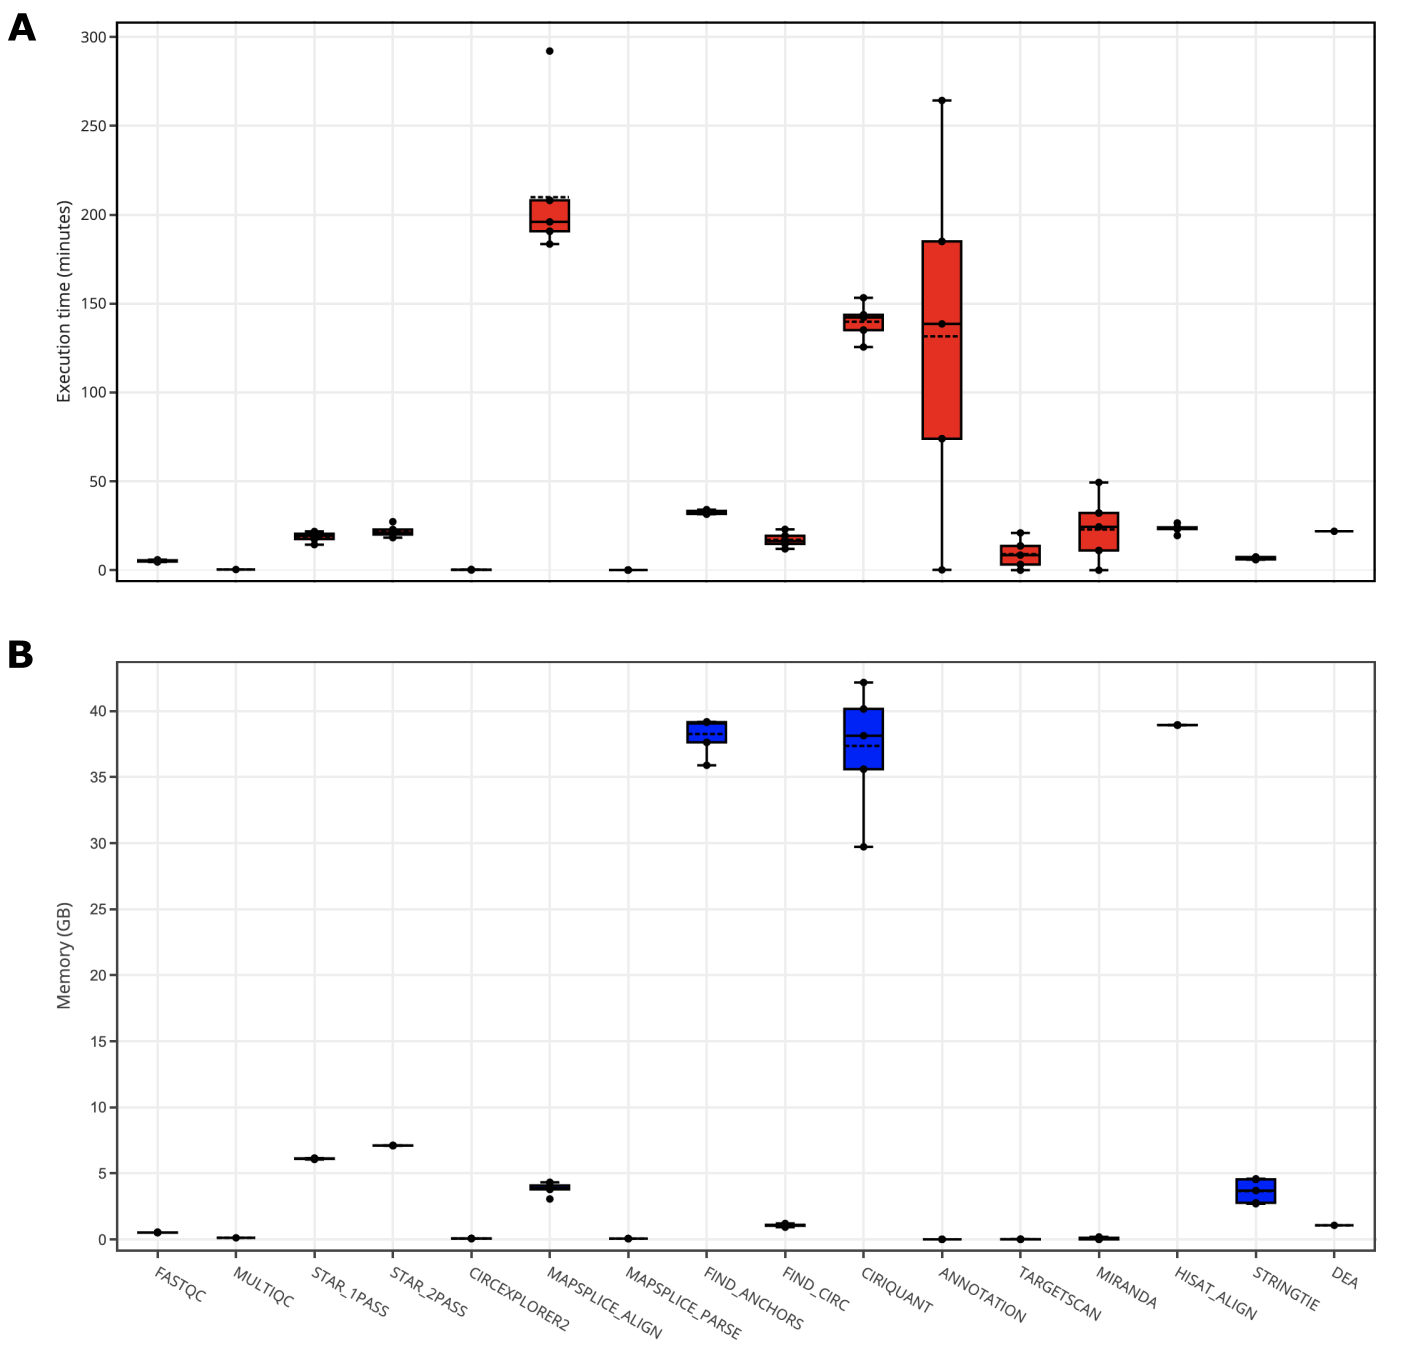
\includegraphics[width=\textwidth]{Chapter2/Figures/figure4.png}
    \vspace{-10mm}
    \caption[Computational performance (PRJNA742881)]{\textbf{nf-core/circrna computational performance (PRJNA742881)}. \textbf{A}. Time elapsed per-process in minutes. \textbf{B.} RAM memory consumed per-process in gigabytes.}
    \label{fig:4}
\end{figure}


\subsubsection{Quantification tool performance}
To assess the performance of nf-core/circrna and it's constituent quantification tools, the workflow was run on a simulated dataset to calculate precision, sensitivity and F1 score performance metrics. The simulated circRNA dataset comprising 1,450,328 synthetic paired-end reads of 101bp in length and 350bp insert size was derived using an overhauled version of CIRIsimulator.pl \cite{CIRI} designed by Zeng et al. \cite{Zeng2017Jun}. This re-worked version of the tool can accept as input circRNA database files from CircBase \cite{circbase}, allowing users to recapitulate \textit{bona fide} circRNAs based on verified back-splice junction coordinates as opposed to the generation of synthetic circRNA reads via the joining of 2 non-collinear exons at random. \par 
7,445 glioblastoma circRNAs were downloaded from circRNADb \cite{circrnadb} and reformatted to conform to CircBase specifications before being supplied as inputs to CIRIsimulator.pl. A total of 7,267 glioblastoma circRNAs were generated by the tool for use in the analysis. As there are no true negatives in the simulated dataset, and all non-true positives are viewed as a false positive, the fraction of relevant instances retrieved by a tool is given by precision, the fraction of relevant instances retrieved relative to the number available instances is given by sensitivity, and the F1 score represents the harmonic mean of precision and sensitivity.  \par
The results of the simulated analysis are given in Table \ref{tab:metrics}. It is important to note sensible filtering parameters were applied to each set of quantification tool results - called circRNAs were required to have at least 2 reads spanning the back-splice junction site. In addition to assessing the performance of each individual quantification tool, circRNAs that had been called by at least two quantification tools via the `\code{-{}-tool\_filter}' parameter were extracted from each set of individual results. The resulting set produced scores of 99.83\%, 96.12\% and 97.94\% for precision, sensitivity and F1, respectively, demonstrating the efficacy of a consensus-based approach to circRNA quantification. 


\begin{table}[h!]
\caption[Performance metrics (glioblastoma dataset)]{Performance metrics of nf-core/circrna quantification tools on the simulated glioblastoma dataset.\label{tab:metrics}}
\centering
\footnotesize
\resizebox{\textwidth}{!}{%
\begin{tabular}{lccccccr}
\toprule
\textbf{Tool} & \textbf{Detected} & \shortstack{\textbf{True}\\\textbf{Positives}} & \textbf{Precision} & \textbf{Sensitivity} & \textbf{F1} & \shortstack{\textbf{Run}\\\textbf{Time}} & \textbf{Memory} \\
\midrule
CIRCexplorer2   & 6270 & 6259 & 99.82\% & 86.13\% & 92.47\% & 7m  & 20 GB \\
CIRIquant       & 6668 & 6663 & 99.93\% & 91.69\% & 95.63\% & 13m & 65 GB \\
circRNA\_finder & 6171 & 5997 & 97.18\% & 82.52\% & 89.25\% & 7m  & 20 GB \\
DCC             & 8397 & 6344 & 75.55\% & 87.30\% & 81.00\% & 34m & 21 GB \\
find\_circ      & 6217 & 6202 & 99.76\% & 85.34\% & 91.99\% & 6m  & 3 GB  \\
MapSplice       & 6155 & 6153 & 99.97\% & 84.67\% & 91.69\% & 9m  & 6 GB  \\
Segemehl        & 4655 & 4558 & 97.92\% & 62.72\% & 76.46\% & 6m  & 50 GB \\
\bottomrule
\end{tabular}%
}
\end{table}


Another useful metric for users to consider when selecting quantification tools for nf-core/circrna is the proportion of common candidates called by each quantification tool. Previously described by Zeng et al. \cite{Zeng2017Jun}, the proportion of common circRNAs shared between two quantification tools $i$ and $j$ can be represented as $C(i,j)$, with the total number of candidates detected by each tool is $N_i$ and $N_j$, respectively. Thus, for tool $i$, the proportion of common candidates is $P(i,j) = C(i,j)/N_i$ and for tool $j$ the proportion of common candidates is $P(j,i) = C(j,i)/N_j$. Pairwise comparisons for all tools in the simulated dataset were generated and represented using a heatmap (Figure \ref{fig:5}). The heatmap can be read in two directions, permitting the bidirectional query of overlapping sets between two quantification tools. When focusing on a specific column, each cell reflects the proportion of common candidates detected by the column tool that were also detected by the corresponding row tool. Conversely, for each row, the cells represent the proportion of common candidates detected by the corresponding column tool that were also recovered by the row tool. \par
Segemehl detected 4,655 circRNAs with 97.92\% precision in the filtered simulated dataset however, it was unable to recover a high proportion of circRNAs detected by other tools, indicating a conservative approach to calling circRNAs. In contrast, DCC detected 8,397 circRNAs, the highest amount detected by any tool in the simulated dataset. DCC produced a high proportion of circRNAs that were not covered by other tools, suggesting a high rate of false positives - confirmed by its 75.55\% precision score. When using the proportion of common candidates to inform quantification tool choices, users should take caution when using DCC by applying sensible filtering parameters to reduce the number of false positives, and supplement Segemehls conservative results with other quantification tools. Encouragingly, CIRCexplorer2, CIRIquant, find\_circ and MapSplice results were all found to have high agreement - a high proportion of circRNA candidates detected by these methods were frequently detected by one another - and high precision scores, indicating robust methods for detecting circRNAs.

\begin{figure}[h!]
    \centering
    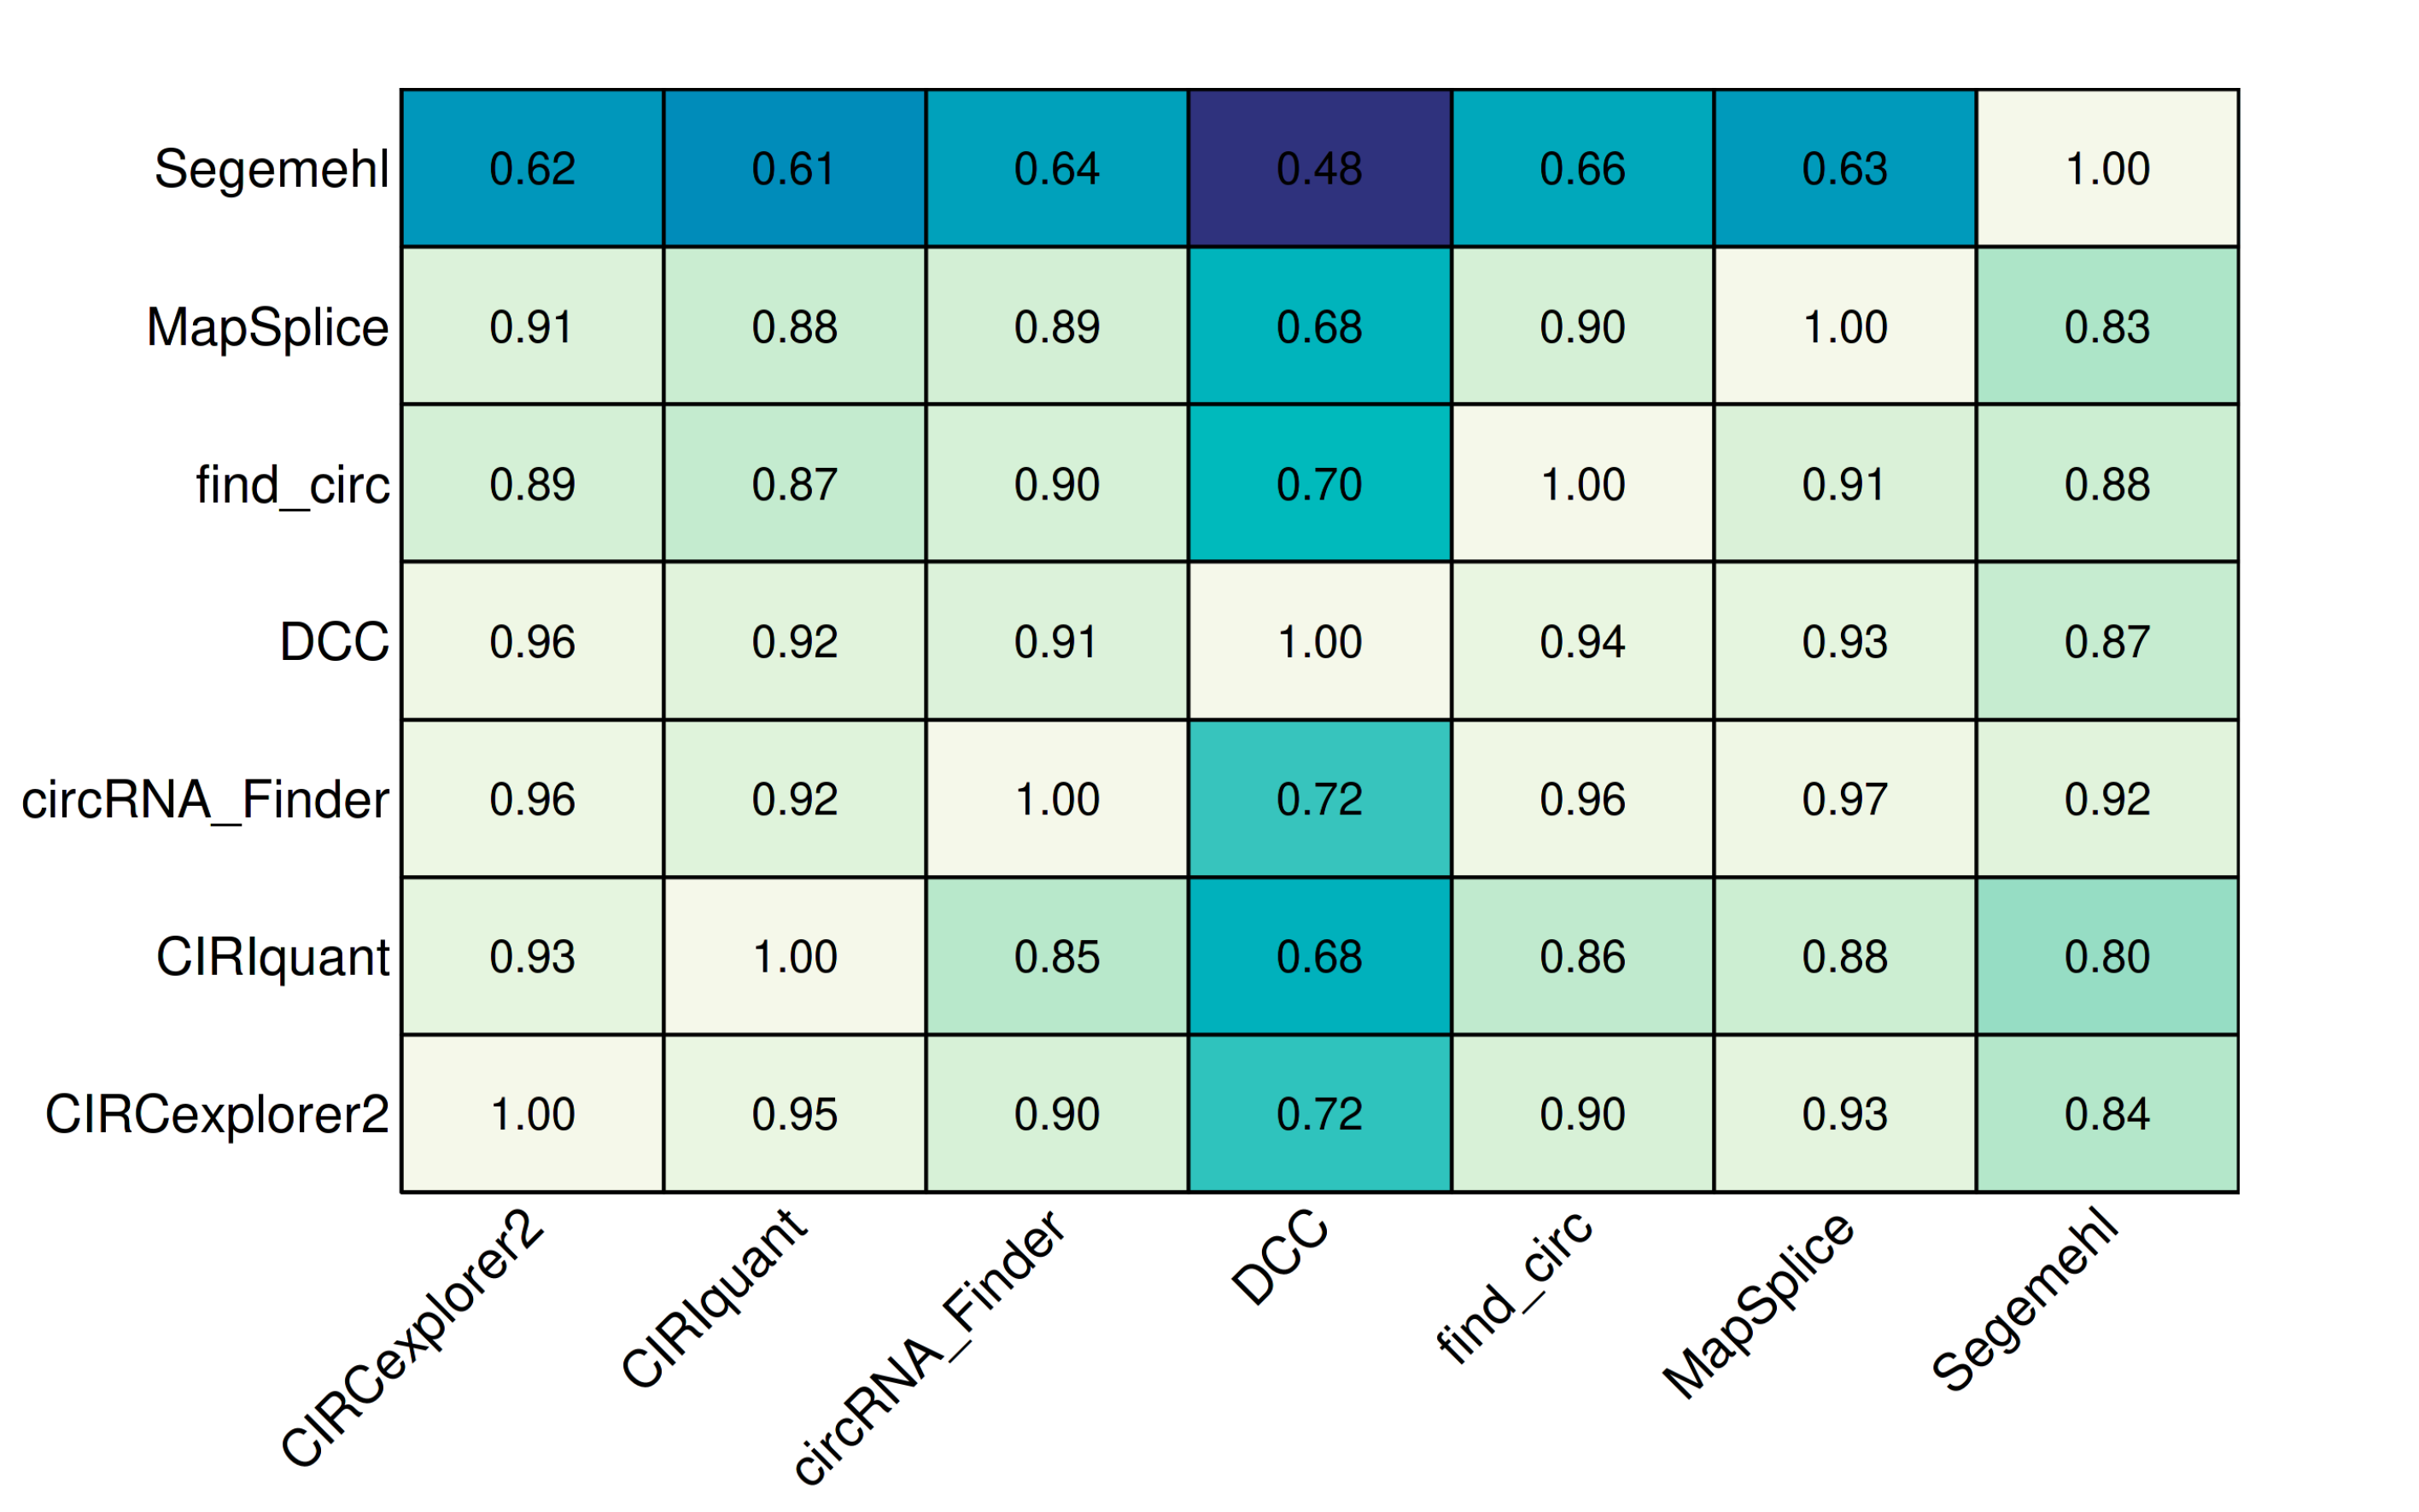
\includegraphics[width=\textwidth]{Chapter2/Figures/figure5.png}
    \vspace{5mm}
    \caption[Proportion of common candidates (glioblastoma dataset)]{The proportion of common circRNA candidates called by each quantification tool in the simulated glioblastoma dataset. }
    \label{fig:5}
\end{figure}

\subsubsection{Optimal parameter selection}
To further advise users on optimal parameter selections for the circrna\_discovery module, we performed an analysis on every possible combination of tools using the simulated dataset coupled with iterative filtering using the `\code{-{}-tool\_filter}' parameter. Our goal was to identify parameters which achieve high performance at the lowest computational cost (i.e requiring the fewest amount of quantification tools in a run).  Briefly, a combinatorics approach was taken whereby each set of quantification tool results were used as inputs to generate all possible combinations: $ _{n}C_{k} = \frac{n!}{(n-k)!}$ where $n = 6$ and $k = 1 \dots 6$, resulting in 126 unique sets after the removal of duplicates. In Figure \ref{fig:6}A, the x-axis depicts the number of quantification tools included in the combinatoric sets, whilst the y-axis displays the corresponding mean value for precision, sensitivty and F1 score. Each colored line represents the value selected for the parameter `\code{-{}-tool\_filter}', requiring circRNAs in sets to be called by at least \textit{n} tools. \par

\begin{figure}[h!]
    \centering
    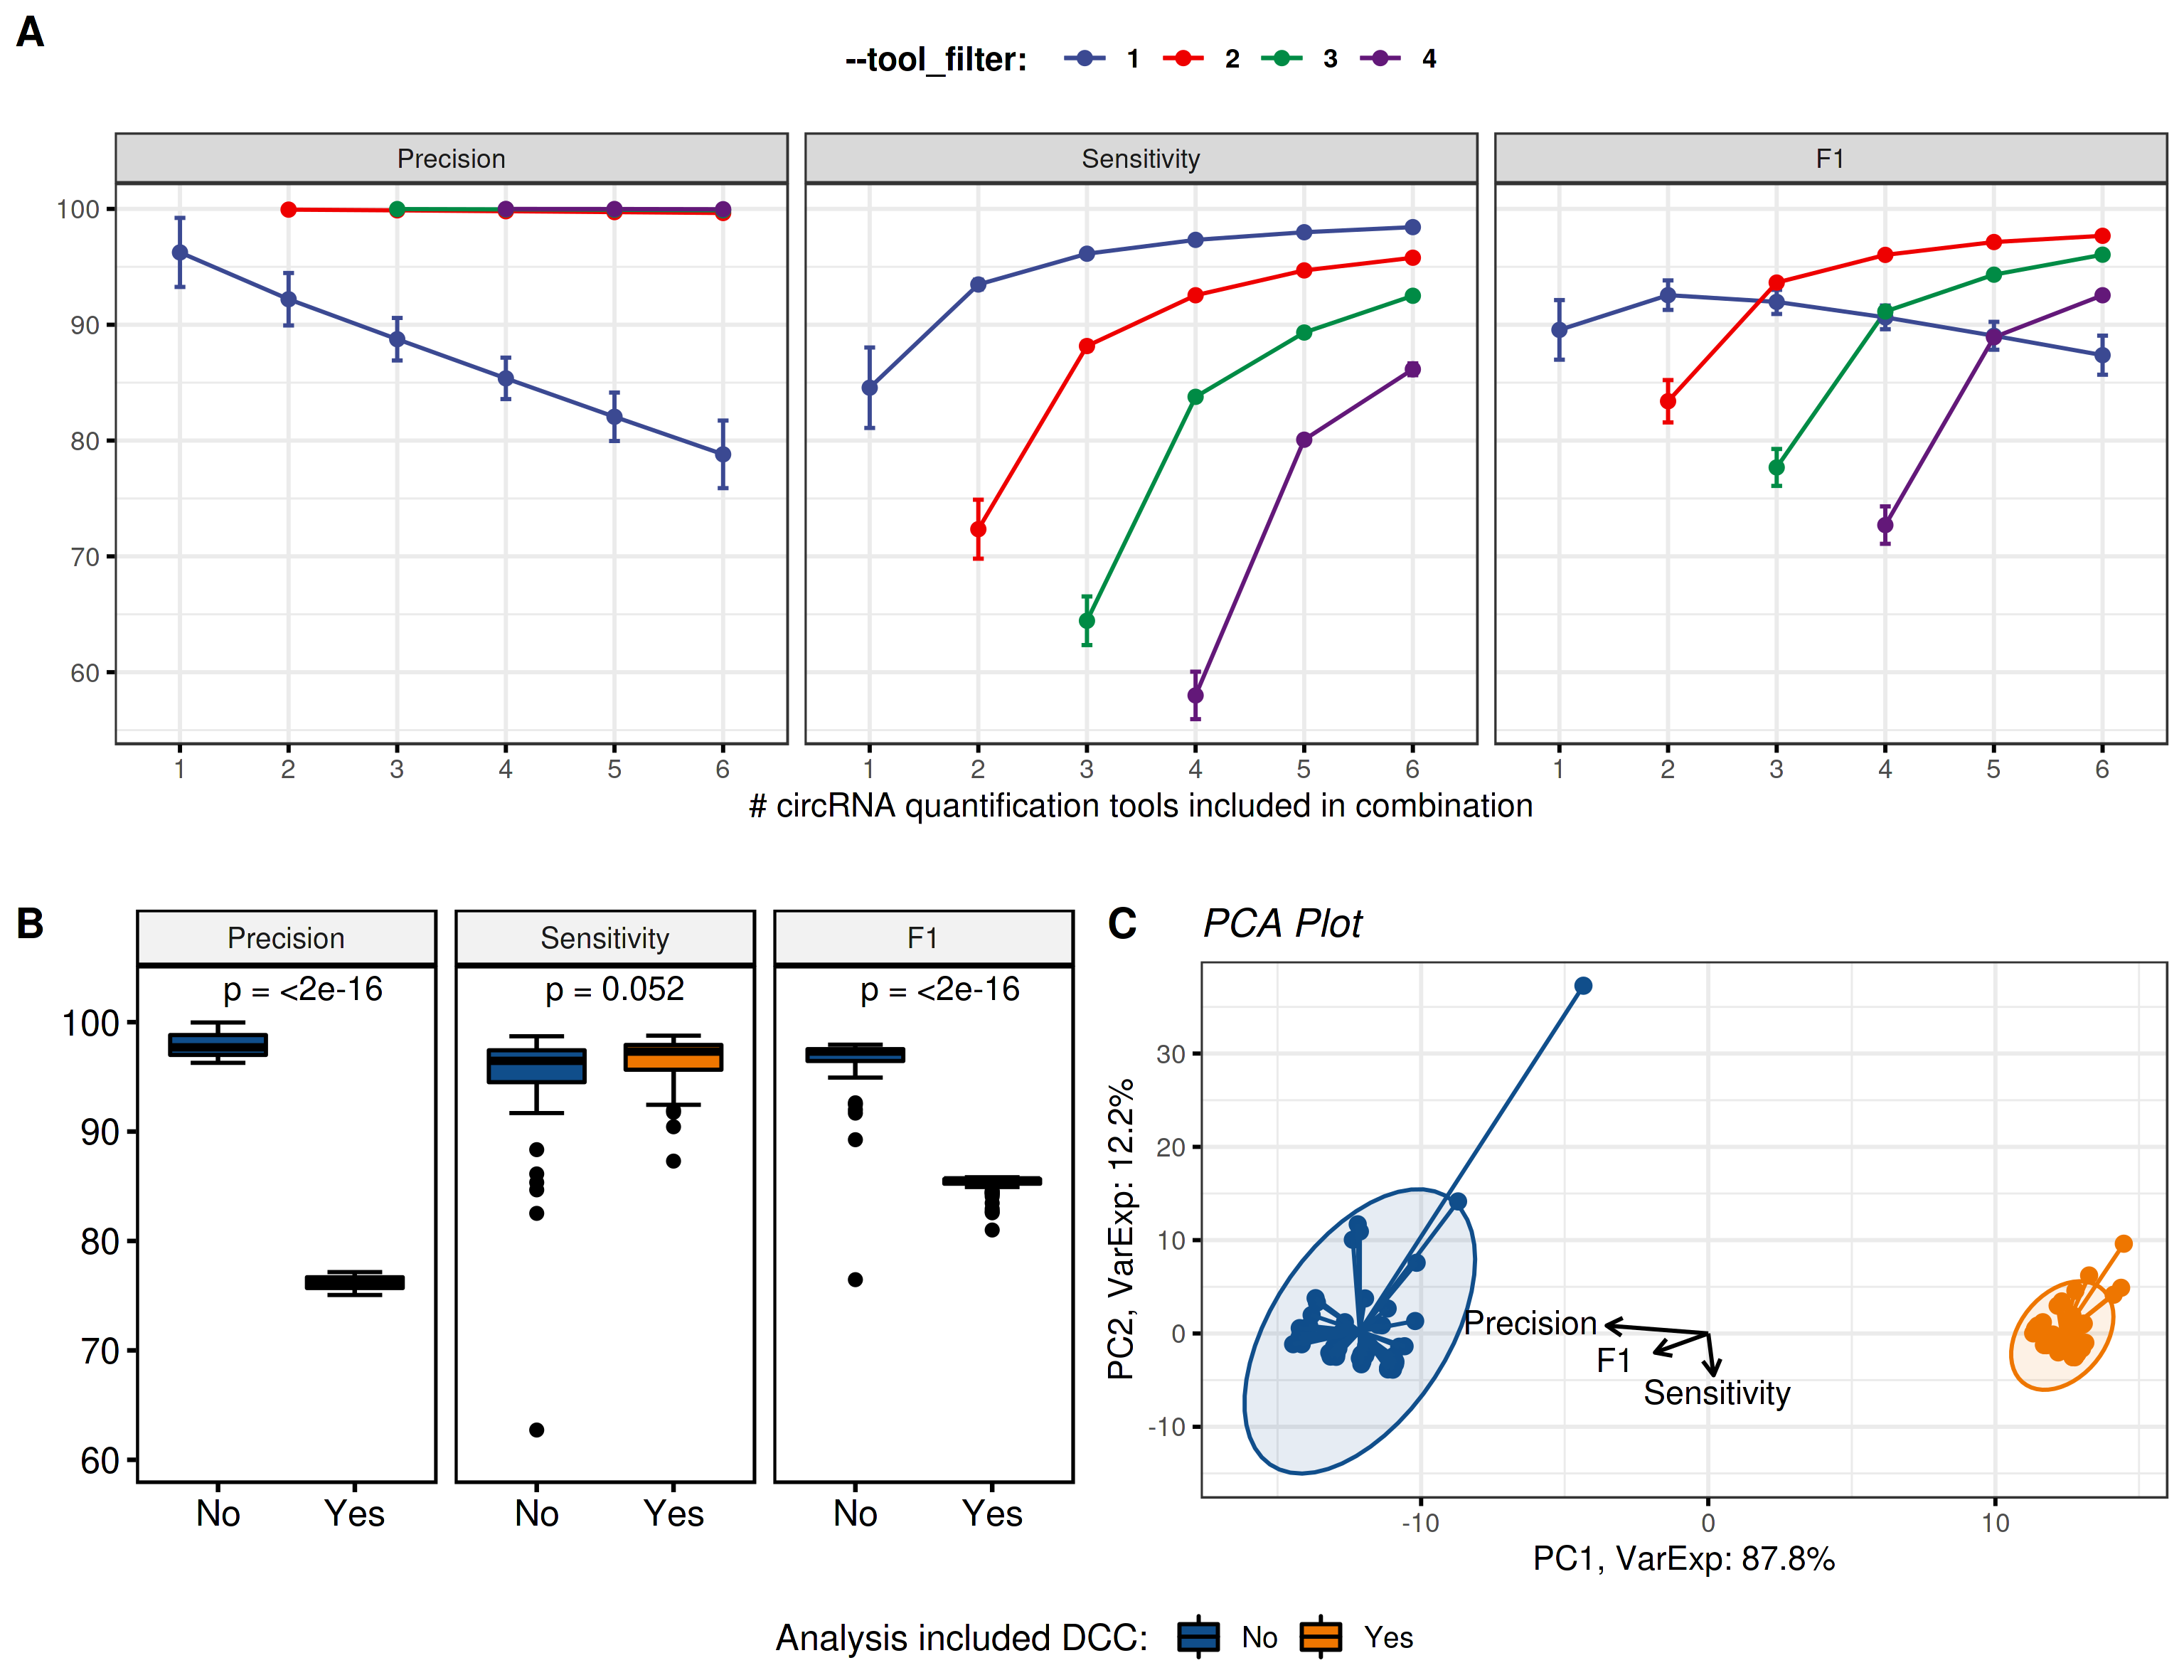
\includegraphics[width=\textwidth]{Chapter2/Figures/figure6.png}
    \vspace{-10mm}
    \caption[Optimal parameter selection]{\textbf{nf-core/circrna optimal parameter selection}(\textbf{A}) Performance metrics for each combinatorics set of results demonstrating the effect of `-{}-tool\_filter' and number of quantification tools included. (\textbf{B}) T-test of all sets including DCC vs. those without DCC for precision, sensitivity and F1 score. (\textbf{C}) Principal component analysis of the sets, displaying the loadings for precision, sensitivity and F1 score.}
    \label{fig:6}
\end{figure}

We observed an inflection point in the lineplot for F1 scores when three quantification tools were selected and `-{}-tool\_filter' was set to two. Increasing the number of quantification tools resulted in minimal performance gains, whilst applying stricter filtering thresholds via `-{}-tool\_filter' greatly reduced sensitivity. The top ten performing combinations of set size three and `-{}-tool\_filter 2' ranked by F1 score are given in Table \ref{table:topcombinations}. Full performance metric results for all iterations of `-{}-tool\_filter' are available in Supplementary file \hyperlink{chp2suppfile1}{1}.
\par 

\begin{table}[t!]
\caption[Top quantification tool combinations]{Top 10 performing quantification tool combinations at the lowest computational cost in the simulated dataset, ranked by F1 score.}
\centering
\footnotesize
\resizebox{\textwidth}{!}{
\begin{tabular}{lccr}
  \toprule
\textbf{Combination} & \textbf{Precision} & \textbf{Sensitivity} & \textbf{F1} \\ 
  \midrule
CIRCexplorer2,CIRIquant,Segemehl & 98.47\% & 97.21\% & 97.83\% \\ 
  CIRIquant,MapSplice,Segemehl & 98.55\% & 96.99\% & 97.76\% \\ 
  CIRCexplorer2,CIRIquant,find\_circ & 99.59\% & 95.89\% & 97.70\% \\ 
  CIRCexplorer2,CIRIquant,MapSplice & 99.74\% & 95.54\% & 97.60\% \\ 
  CIRIquant,find\_circ,MapSplice & 99.70\% & 95.57\% & 97.59\% \\ 
  CIRCexplorer2,find\_circ,Segemehl & 98.33\% & 96.57\% & 97.45\% \\ 
  CIRCexplorer2,MapSplice,Segemehl & 98.50\% & 96.41\% & 97.44\% \\ 
  CIRIquant,find\_circ,Segemehl & 98.37\% & 96.46\% & 97.41\% \\ 
  CIRCexplorer2,find\_circ,MapSplice & 99.61\% & 95.28\% & 97.40\% \\ 
  CIRCexplorer2,CIRIquant,circRNA\_finder & 97.51\% & 97.18\% & 97.35\% \\ 
   \midrule
\end{tabular}}
\label{table:topcombinations}
\end{table}

Furthermore, we were interested in identifying quantification tools that negatively impacted the performance in each of the sets. Clustering analysis of the matrix containing precision, sensitivity and F1 score for all 126 unique sets revealed sets containing results from the tool DCC negatively impacted performance metrics. This was formally tested using a t-test (Figure \ref{fig:6}B) and depicted using principal component analysis whereby the first principal component clearly displays sets containing DCC and negatively correlated with the loadings for precision and F1 score, respectively. DCC is the only quantification tool that utilises STAR 2-pass mode, greatly increasing the sensitivity around splice junction sites at the cost of false positives \cite{Engstrom2013Dec}. Users should take this information into consideration when selecting quantification tools for their own analysis and apply sensible filtering parameters to reduce spurious calls. 


\subsection{Conclusion}
nf-core/circrna is the first portable workflow capable of performing the quantification, miRNA target prediction and differential expression analysis of circRNAs in a single execution. Its ease of use greatly reduces the barrier to entry for users seeking to characterise the role of circRNAs in the ceRNA network. We look forward to the workflows release and subsequent engagement with the research community - as the field of circRNA analyses advances, we will effort to incorporate user feedback, suggestions and requests to maintain the vitality and contemporary status of the workflow. 

\subsection{Supplementary Files}
\hypertarget{chp2suppfile1}{}

Supplementary File 1 is available online at the following \href{https://link.springer.com/article/10.1186/s12859-022-05125-8#Sec16}{link}
{\Huge \bfseries \noindent Chapter 4}
\vspace{-1em} 
\section*{\LARGE pycircdb: integrated circRNA database annotation for computational workflows}
\addcontentsline{toc}{section}{4\quad pycircdb: integrated circRNA database annotation for computational workflows}
\setcounter{section}{4}
\setcounter{subsection}{0}  % reset so next \subsection is 2.1
\renewcommand{\chapternum}{4}

% Reset figure/table numbering after chapter 4 supplementary overrides
\renewcommand{\thefigure}{\chapternum.\arabic{figure}}
\setcounter{figure}{0}
\renewcommand{\thetable}{\chapternum.\arabic{table}}
\setcounter{table}{0}

\begin{center}
    \textit{The contents of this chapter have been accepted for publication in Bioinformatics Advances}
\end{center}



\subsection*{Abstract}
\textbf{Motivation}: Currently, multiple databases exist for the annotation of circular RNAs, providing descriptions of their genomic features, FASTA sequences, predicted microRNA targets and RNA-binding protein interactions. Despite the availability of these resources, annotation remains cumbersome. Conflicting identifiers and genomic coordinates for circular RNAs across databases pose a challenge to reproducibility for users. Furthermore, current databases primarily provide access via web-based graphical user interfaces, bulk downloads and limited programmatic access, rendering their use in computational workflows challenging. \\
\textbf{Results}: We present pycircdb, a Python command-line interface tool that accepts genomic coordinates of human circular RNAs as input, facilitating rapid queries of multiple curated circRNA databases for reproducible annotation. Each pycircdb database has been normalised to a common 0-based representation and cross-mapped between the hg19 and hg38 assemblies, accepting as input circular RNA coordinates from 0-based and 1-based sources using a tolerant matching strategy. pycircdb utilises Apache Hamilton in conjunction with Parquet files, providing a modular, parallelised workflow with minimal disk space requirements.   \\
\textbf{Availability}: pycircdb is available for download via PyPI \href{https://pypi.org/project/pycircdb/}{https://pypi.org/project/pycircdb} under the GPL-3.0 license with source code and documentation available at \href{https://github.com/BarryDigby/pycircdb}{https://github.com/BarryDigby/pycircdb} and \href{https://pycircdb.readthedocs.io/en/latest/}{https://pycircdb.readthedocs.io/en/latest}, respectively.\\


\subsection{Introduction}

Initially discovered in plant viroids \cite{Sanger1976}, yeast mitochondrial RNAs \cite{Arnberg1980Feb}, and the hepatitis $\delta$ virus \cite{Kos1986Oct}, circular RNAs (circRNAs) were believed to be by-products of aberrant splicing or intermediates discarded from intron-lariat debranching \cite{Cocquerelle1993Jan}. Advancements in bioinformatics techniques and RNA-Sequencing protocols enabled the detection of circRNAs, with interest in the field invigorated when a landmark study by Salzman et al. identified circRNAs in hyperdiploid acute lymphoblastic leukaemia diagnostic bone marrow samples \cite{Salzman2012}. 

Originating from the same precursor messenger RNA as their linear RNA transcripts, circRNAs are formed through a process known as back-splicing in which a downstream 5' splice donor site is reversely joined to an upstream 3' splice acceptor site, forming a covalently closed loop structure \cite{Jeck2012Dec}. Although the functions of most circRNAs have yet to be revealed, evidence suggests circRNAs harbour functionally active and evolutionarily conserved microRNA (miRNA) response elements within their mature spliced sequence \cite{Hansen2013Mar}, suggesting a regulatory role within the competing endogenous RNA network by sequestering endogenous miRNAs \cite{Denzler2014Jun}. Furthermore, circRNAs can form a scaffold with RNA-binding protein(s) (RBP), acting as modulators of transcription and splicing, and as templates for translation \cite{Shi2025}.

\begin{figure*}[ht!]
    \centering
    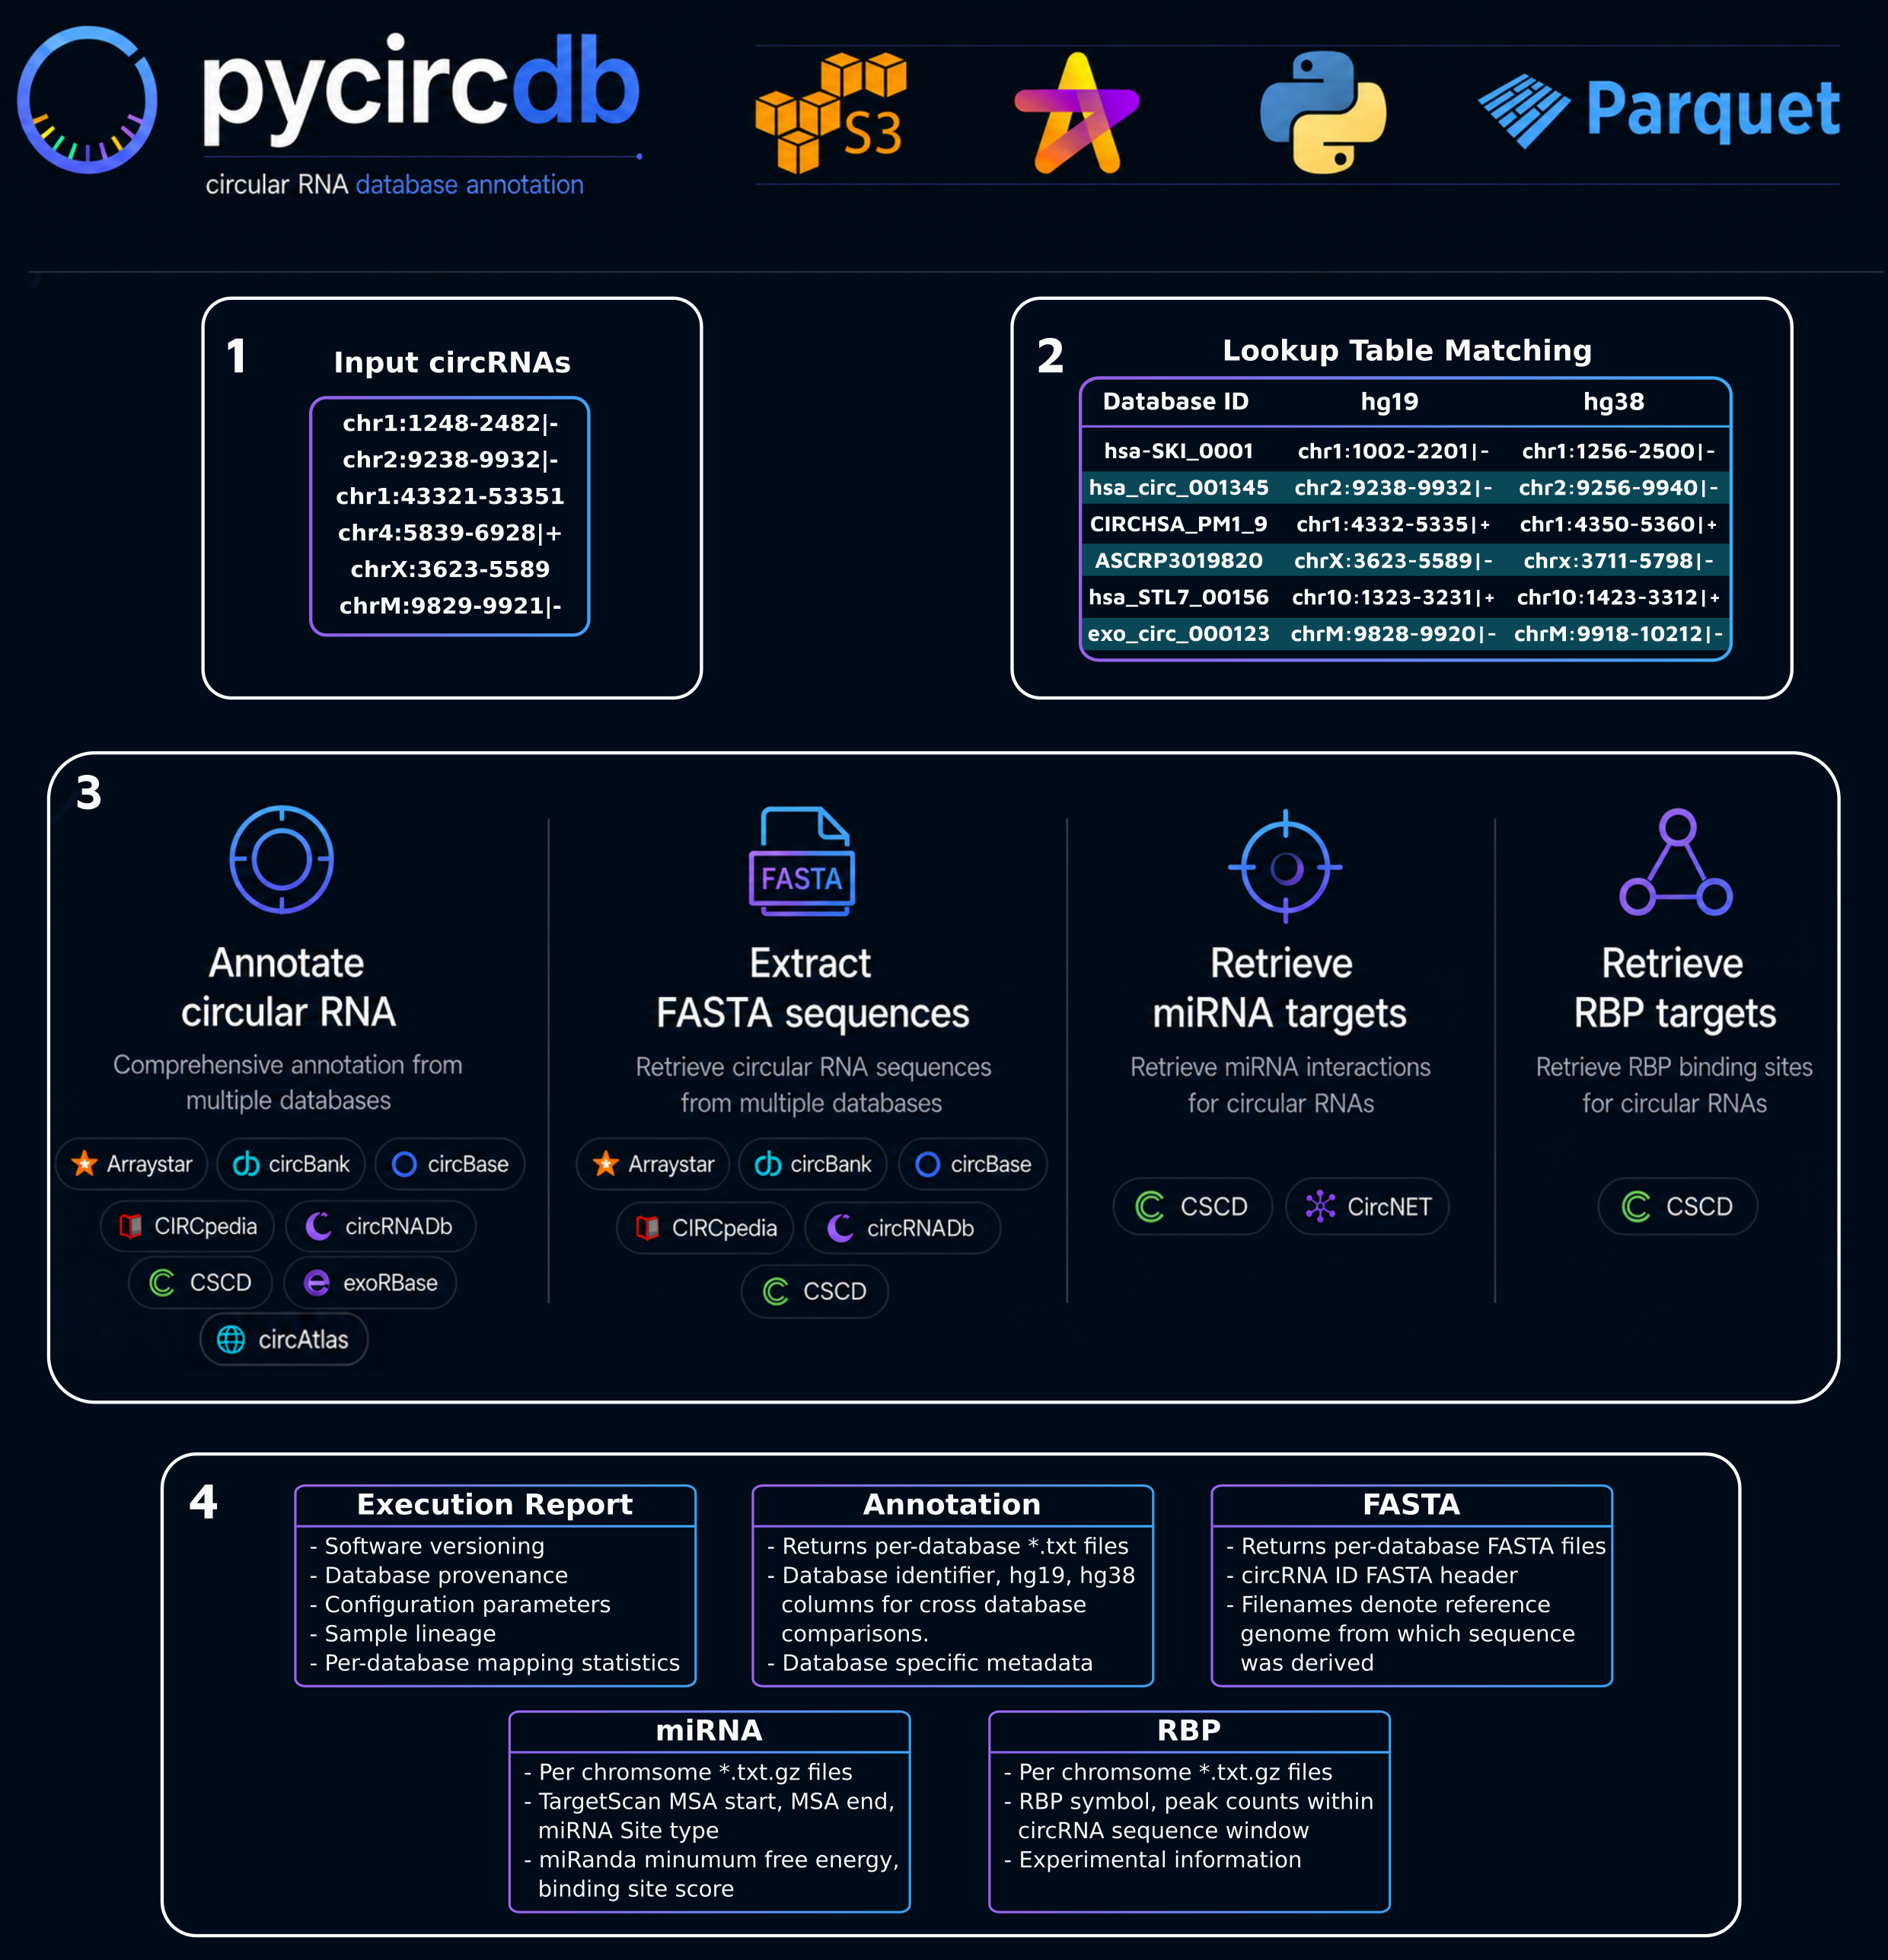
\includegraphics[width=\linewidth]{Chapter4/Figures/Figure_1.png}
    \caption[Overview of pycircdb Python tool]{\textbf{Overview of the pycircdb Python tool}. 1: Input hg19 circRNAs in \texttt{chr:start-end$\vert$strand} format provided in a single-column text file (strand optional, configuration file not shown). 2: Perform matching against pycircdb lookup tables. Exact matching (\texttt{chr2:9238-9932$\vert$-}), strand ambiguous matching (\texttt{chrX:3623-5589}) and tolerant coordinate matching (\texttt{chrM:9829-9921$\vert$-}). 3: Lookup hits are used as inputs to the \texttt{annotate}, \texttt{fasta}, \texttt{mirna} and \texttt{rbp} modules. 4: Summary of output files generated by pycircdb.}
    \label{fig:pycircdb}
\end{figure*}

Due to their circular topology, circRNAs lack a poly(A) tail and 5' and 3' ends, conferring resistance to RNase degradation, resulting in a stable RNA structure with a higher half-life compared to their linear counterparts \cite{Salzman2012}. Several studies have identified circRNAs in human biofluids, including saliva, plasma, serum, and in exosomes, making them attractive candidate biomarkers for non-invasive liquid biopsy approaches \cite{Memczak2015}. circRNAs further exhibit stage and tissue-specific expression \cite{Gruner2016} and are dysregulated across a wide range of cancers \cite{Conn2024Sep}.

These discoveries have motivated the development of numerous bioinformatics pipelines for circRNA detection, and in turn, dedicated databases have emerged to consolidate the circRNAs reported by these pipelines across human studies \cite{Digby2024Dec}. Whilst these databases are valuable resources, they suffer from a lack of a standardised naming convention for their circRNA identifiers. For example, the hg19 circRNA \texttt{chr1:27087346-27089776$\vert$+} returns the following identifiers: ASCRP3003018 (Arraystar), hsa-ARID1A\_0002 (circAtlas), hsa\_ARID1A\_0003300 (circBank), hsa\_circ\_0006913 (circBase). Compounding this problem is the fact that individual databases are built against different reference genome assemblies and adopt inconsistent coordinate conventions, mixing 0-based and 1-based systems. Most significantly, a subset of databases support only single circRNA queries, making systematic annotation of experimentally detected circRNAs an arduous process.

No existing resource addresses all three barriers (Supplementary Table \ref{pycircsupptab1}). Individual databases provide web-based interfaces or bulk downloads, but none offers a unified programmatic interface that queries multiple databases concurrently, normalises coordinates across genome assemblies and base conventions, and returns results in a format directly consumable by downstream analysis scripts. BioMart \cite{biomart} provides general genomic annotation but has not yet integrated circRNA-specific resources; circAtlas \cite{circinteractome} in addition to other databases, supports only single-query submissions; the CircFunBase API accepts only single circRNA queries; and bulk-download files from individual databases still require users to independently reconcile conflicting identifiers and coordinate systems before any cross-database comparison is possible.

We present pycircdb, a Python tool that takes as input hg19 or hg38 circRNA coordinates from multiple samples and performs a lookup of nine manually reformatted circRNA databases, returning circRNA annotations, FASTA sequences, and precomputed miRNA and RBP interactions (Figure \ref{fig:pycircdb}). As a command-line interface (CLI) tool, pycircdb can be integrated into computational workflows as part of a quantification pipeline or used as a post-hoc tool to query circRNAs. pycircdb is open-source, with source code freely available at \href{https://github.com/BarryDigby/pycircdb}{https://github.com/BarryDigby/pycircdb}. 


\subsection{Implementation}
\subsubsection{Database Design}
Publicly available human hg19/hg38 circRNA database files from Arraystar, circAtlas \cite{circatlas}, circBank \cite{circbank}, circBase \cite{circbase}, CircNet \cite{circnet}, CIRCpedia \cite{circpedia}, circRNADb \cite{circrnadb}, CSCD \cite{CSCD2} and exoRBase \cite{exoRBase} were downloaded from their respective sources (Table \ref{pycircdbsumm}). Reformatting of each database was performed manually, encompassing conversion of 1-based genomic coordinates to a common 0-based representation and cross-mapping between hg19 and hg38 using UCSC liftOver \cite{ucscliftover} with the \texttt{hg19ToHg38.over.chain.gz} and \texttt{hg38ToHg19.over.chain.gz} chain files at default settings. CSCD records required additional handling. Briefly, CSCD records detected by CIRI and circRNA\_finder can have multiple entries for a record: 1) a circRNA record with $\geq$2 quantification tools as evidence, of which CIRI and/or circRNA\_finder are members; 2) the same record reported on the antisense strand with only circRNA\_finder as evidence; and 3) a 1-based version of the record supported by only CIRI. We removed the 1-based CIRI entries and circRNA\_finder antisense entries to prevent duplicate annotation records in the pycircdb output. The removal of antisense circRNA\_finder entries is validated by the circBase identifiers retained in CSCD: since circBase identifiers are strand-specific, a circBase ID cannot legitimately annotate entries on opposing strands. We therefore applied the same filtering logic to analogous CIRI and circRNA\_finder entries lacking a circBase identifier. During the conversion from hg19 to hg38, segmentally duplicated and repetitive-rich regions within the genome produced `one-to-many' hg19 to hg38 coordinates, which are accounted for in pycircdb by retaining multi-mapped coordinates rather than collapsing identifiers to one region (Supplementary Figure \ref{pycircsuppfig1}); the number of records successfully mapped, failing liftover, and producing one-to-many mappings is reported per database in Supplementary Table \ref{pycircsupptab1}.

\begin{table*}[!ht]
\centering
\caption[Summary of circRNA databases integrated in pycircdb and their use in corresponding modules]{\textbf{Summary of circRNA databases integrated in pycircdb and their use in corresponding modules}. `Entries' is the total number of circRNA records in each pycircdb annotation lookup table. CSCD provides 177,600,389 circRNA-miRNA and 106,438,146 circRNA-RBP entries, respectively. For databases with circRNA sequences (FASTA module), the number of records is identical to `Entries' and is therefore not repeated. Liftover failure and one-to-many mapping counts per database are reported in Supplementary Table \ref{pycircsupptab2}}
\label{pycircdbsumm}
\resizebox{\textwidth}{!}{%
\begin{tabular}{llcllrcccc}
\toprule
Database & Reference & Coordinates & Version & Accessed & Entries & Annotation & FASTA & miRNA & RBP \\
\midrule
Arraystar   & hg19 & 1-based & 2.0   & Jan 2025 & 13,154    & \cmark & \cmark & \xmark & \xmark \\
circAtlas   & hg38 & 1-based & 3.0   & Jan 2026 & 768,986   & \cmark & \xmark & \xmark & \xmark \\
circBank    & hg19 & 1-based & 1.0   & Jan 2026 & 828,802   & \cmark & \cmark & \xmark & \xmark \\
circBase    & hg19 & 0-based & 1.0   & Jan 2026 & 92,369    & \cmark & \cmark & \xmark & \xmark \\
CircNet     & hg19 & 1-based & 2.0   & Jan 2026 & 6,913,950 & \xmark & \xmark & \cmark & \xmark \\
CIRCpedia   & hg38 & 0-based & 3.0   & Oct 2025 & 849,495   & \cmark & \cmark & \xmark & \xmark \\
circRNADb   & hg19 & 1-based & 1.0   & Mar 2026 & 32,942    & \cmark & \cmark & \xmark & \xmark \\
CSCD        & hg38 & 1-based & 2.0   & Jan 2026 & 2,749,897 & \cmark & \cmark & \cmark & \cmark \\
exoRBase    & hg38 & 1-based & 3.0   & May 2026 & 126,816   & \cmark & \xmark & \xmark & \xmark \\
\bottomrule
\end{tabular}%
}
\end{table*}

Next, lookup tables were constructed for each database containing the original database identifier alongside the corresponding hg19 and hg38 coordinates (Supplementary Figures \ref{pycircsuppfig2} and \ref{pycircsuppfig3}; Supplementary Tables \ref{pycircsupptab3} and \ref{pycircsupptab4}). The lookup tables are used to match user-provided circRNA inputs and serve as the basis for querying the annotation, FASTA, miRNA, and RBP database tables based on user-supplied commands supplied at runtime. \par

Annotation, miRNA and RBP tables were modified to include both hg19 and hg38 lookup keys in addition to their original columns, whilst FASTA tables were reformatted to a two-column format containing the original database identifier and the circRNA sequence. FASTA sequences were retained in their original reference genome sequence; Arraystar, circRNADb, circBank, and circBase are hg19-based, while CIRCpedia and CSCD are hg38-based. Sequences are retrieved exactly as provided by the original databases and are not regenerated from input coordinates. The reference assembly is encoded in each output filename (e.g. \texttt{arraystar\_hg19.fasta}, \texttt{cscd\_hg38.fasta}), making the source assembly unambiguous without requiring cross-reference to external documentation. Summaries of shared circRNA coordinates in FASTA database tables are available in Supplementary Figure 4 and Supplementary Table 5, respectively.


All lookup, annotation, sequence, miRNA and RBP tables are stored as Apache Parquet files in a publicly accessible AWS S3 bucket. The complete database occupies 3.6 GB of disk space; however, pycircdb only downloads the files required for a given run - those corresponding to the databases specified by the user and, for the miRNA and RBP resources, only the chromosome tables matching the chromosomes present in the input data.

Databases were selected on the basis of publicly available human data for bulk download. Several candidate resources were evaluated but excluded: CircInteractome was omitted because its circRNA set overlaps substantially with circBase without providing additional annotation; CircFunBase was excluded owing to its limited human entry count (3,799 records at the time of access); and multiple databases were inaccessible (Supplementary Table \ref{pycircsupptab1}). Databases providing only sample-level membership information without coordinate-level annotation (MiOncoCirc, NeuroCirc) were also excluded as they would not enrich pycircdb outputs. Database files are versioned independently of the pycircdb package using a \texttt{db\_version.txt} file shipped with the package. This file specifies the current database version and is used to resolve the correct S3 directory at runtime (e.g. \texttt{v1\_0/} for database version 1.0, \texttt{v1\_1/} for 1.1). Prior database snapshots are retained on S3 indefinitely, ensuring that any past release of pycircdb continues to query the same database it was originally distributed with. Database updates are communicated via GitHub releases and a version badge in the repository README.

To confirm that coordinate-based lookup correctly resolves database-specific identifiers, the six circRNAs comprising pycircdb's \texttt{init-demo} demonstration dataset - each present in all eight annotation databases - were queried; pycircdb returned the expected identifier in every database without exception (Supplementary Table \ref{pycircsupptab6a}).


\subsubsection{pycircdb Design}
At its core, pycircdb utilises Apache Hamilton, a declarative framework that maps dependencies between individual Python functions to construct a directed acyclic graph (DAG). This approach facilitates configuration-driven, parallel execution of the DAG code. pycircdb's codebase is composed of several modules: 1) ingest user inputs, download all lookup tables and return lookup hits; 2) download the requisite annotation, FASTA, miRNA and RBP files based on user command parameters, and for database files split by chromosome, downloading only the partitions corresponding to chromosomes represented in the lookup hits; 3) pool hg19/hg38 circRNA coordinates from each lookup table for use in downstream subsetting steps; 4) subset the annotation database tables and write to files; 5) subset the FASTA database tables using pooled circRNA coordinates and their corresponding database identifiers and write to files; 6) subset the miRNA database tables and write to gzip-compressed files; and 7) subset the RBP database tables and write to gzip-compressed files. 

Given that circRNA quantification tools report coordinates in either 0-based or 1-based outputs and, in some cases, omit strand information, pycircdb applies a tolerant coordinate matching strategy to accommodate the output of any quantification tool run on human samples once converted to the expected format. For each input circRNA, three candidate start positions are generated (original, $-1$\,bp, $+1$\,bp) whilst the end coordinate is held fixed, capturing the single-base offset introduced by 0-based versus 1-based conventions. When strand is provided, matching is performed exactly against the database coordinate including strand; when strand is omitted, the strand suffix is stripped from database entries prior to matching, and all strand information at matching positions is returned. Users need only consolidate the chromosome, start, end and (optionally) strand into pycircdb's \texttt{chr:start-end$\vert$strand} format for inputs. Chromosome names require the \texttt{chr} prefix; supported chromosomes are chr1--chr22, chrX, chrY and chrM. chrM is supported by the \texttt{annotate} and \texttt{fasta} commands but excluded from the \texttt{mirna} and \texttt{rbp} modules, as chromosome-level predictions for chrM are absent from the source databases. 

Each matched entry produces one output row per circRNA-database pair in the designated output `database hits' file; a single input circRNA may return multiple rows where it maps to multiple coordinates via one-to-many liftover. Currently, \texttt{pycircdb} documents multi-mapping circRNAs in the execution report summary file; however, coordinate-tolerant matches and strand-ambiguous matches are not distinguished in outputs

\subsubsection{pycircdb Invocation}
pycircdb is configured via a JSON file, specifying both global and sample-level parameters for a workflow run. 

Global parameters include: 1) \texttt{max\_tasks}: the number of concurrent threads for Apache Hamilton parallelism (default: 1); 2) \texttt{output\_dir}: the output directory to write results to using relative or full paths (default: \texttt{results/}); and 3) \texttt{tmp\_dir}: the directory used to store downloaded database files. When running on Cloud/HPC, we recommend using a shared storage space accessible to other users for subsequent runs (default: \texttt{tmp/}).

Sample parameters can be specified multiple times under the \texttt{samples} parent key. Each child collection includes the sample name used to name the subdirectories of the output directory, the \texttt{file\_path} parameter providing the relative or full path to the input sample file containing circRNAs and the \texttt{reference} parameter specifying the reference genome used to generate the input circRNAs (hg38 or hg19).

pycircdb contains global click options, click commands and click command-level options. Global options include \texttt{-c/--config} denoting the configuration file, which is mandatory. The \texttt{-v/--verbose} option is set to 0, 1 and 2, respectively, with higher integers representing more verbose output. Five commands are available to users: 1) \texttt{init-demo}: creates a minimal test configuration file complete with a toy dataset; recommended for first-time users to inspect outputs generated by pycircdb; 2) \texttt{annotate}: return all database hits from Arraystar, circAtlas, circBank, circBase, CIRCpedia, circRNADb, CSCD and exoRBase, providing comprehensive information of circRNAs; 3) \texttt{fasta}: return all predicted circRNA sequences from Arraystar, circBank, circBase, CIRCpedia, circRNADb and CSCD; 4) \texttt{mirna}: retrieve precomputed circRNA-miRNA interactions from CircNet and CSCD, generated using miRanda, PITA and TargetScan; and 5) \texttt{rbp}: retrieve precomputed circRNA-RBP interactions from CSCD database. Both the \texttt{annotate} and \texttt{fasta} commands accept the command-level option \texttt{-d/--database}, where users can specify specific databases to query instead of the default of all databases. The \texttt{mirna} command accepts the option \texttt{-a/--algorithm}, permitting users to subset circRNA-miRNA results to miRanda, PITA or TargetScan, or any combination thereof (Supplementary Table \ref{pycircdbsupptab7}). 

\begin{table*}[!ht]
\centering
\caption[pycircdb benchmarking results]{\textbf{pycircdb benchmarking results.} Inputs marked $^\dagger$ are high-confidence circRNA candidates ($\geq$3 back-splice junction reads, detected by $\geq$3 of seven quantification tools); remaining inputs are circRNAs with no filtering applied for performance scaling assessment. Annotation and FASTA columns report unique circRNAs across results (rate of annotation multi-mapping circRNAs are in superscript); miRNA and RBP report unique hg38 coordinates with miRNA/RBP interactions. Database files (3.6\,GB) were pre-cached; download time is excluded.}
\label{pycircbenchmarking}
\resizebox{\textwidth}{!}{%
\begin{tabular}{llrrrrrr}
\toprule
Input & Annotation & FASTA & miRNA & RBP & Wall clock (s) & Peak RAM (GB) & Results Disk (MB) \\
\midrule
100$^\dagger$     &    96 &    96 &     96 &    96 &  13.7 & 2.3 &   2.6 \\
1,000$^\dagger$   &   974 &   974 &   964 &   962 &  16.2 & 2.5 &  23.4 \\
10,000$^\dagger$  & 9,789\textsuperscript{(7)} & 9,789 &  9,685 &  9,685 & 25.8 & 2.7 & 228.8 \\
100,000           & 14,123\textsuperscript{(30)} & 14,104 & 13,273 & 13,223  & 35.0 & 3.1 & 240.5 \\
200,000           & 28,307\textsuperscript{(45)} & 28,271 & 26,368 & 26,241  & 52.9 & 3.3 & 469.8 \\
300,000           & 42,530\textsuperscript{(63)} & 42,476 & 39,298 & 39,108  & 66.7 & 3.8 & 690.7 \\
\bottomrule
\end{tabular}%
}
\end{table*}

\subsubsection{pycircdb outputs}
pycircdb produces five categories of output, all written to a user-specified directory.

\textbf{Execution report.}
A plain-text execution report (\texttt{execution\_report\_<timestamp>.txt}) is generated after every run, recording the run timestamp, software and database bundle versions, the configuration used, per-sample inputs and reference genomes, the databases and miRNA prediction algorithms selected, and database provenance (native genome build, version, and access date). Per-database mapping statistics are provided as the ratio of input to database hits (one-to-one). Multi-mappers, if present, are also reported.

\textbf{Annotation.}
For each selected annotation database (Arraystar, circAtlas, circBank, circBase, CIRCpedia, circRNADb, CSCD, and exoRBase) a tab-delimited file is written containing the database-native circRNA identifier, coordinates in both hg19 and hg38, and database-specific metadata. Common fields across databases include chromosomal coordinates, strand, host gene symbol, circRNA biotype (exonic, intronic, intergenic, or exon-intron circRNA), and transcript of origin where available. CSCD additionally reports subcellular localisation, detection algorithms, read counts per sample, alternative splicing events, and circular-to-linear expression ratios.

\textbf{FASTA sequences.}
For databases that provide spliced circRNA sequences (Arraystar, circBank, circBase, CIRCpedia, circRNADb, and CSCD), a FASTA file is written containing the circular RNA sequence for each circRNA.

\textbf{miRNA interactions.}
Predicted miRNA binding sites are reported in a per-chromosome \texttt{*.txt.gz} tab-delimited file aggregating results from CircNet and CSCD across the miRanda, PITA, and TargetScan algorithms, with columns for binding site coordinates, site type, score, and minimum free energy where available.

\textbf{RBP interactions.}
RBP interactions derived from CSCD are reported in a per-chromosome \texttt{*.txt.gz} tab-delimited file containing the RBP symbol, binding site coordinates, number of RBPs predicted to bind at the site coordinates and tissue context (normal, cancer, or common).

A full description of pycircdb outputs, including detailed descriptions of each database column, is provided in the documentation: \href{https://pycircdb.readthedocs.io/en/latest/outputs.html}{https://pycircdb.readthedocs.io/en/latest/outputs.html}.

\subsubsection{pycircdb Testing and Performance}
pycircdb is tested via a cross-platform continuous integration (CI) pipeline on GitHub Actions, executing all five commands (\texttt{init-demo}, \texttt{annotate}, \texttt{fasta}, \texttt{mirna} and \texttt{rbp}) across Ubuntu, macOS, and Windows using Python 3.10--3.14. Benchmarking was performed using circRNA candidates from two human glioblastoma RNA-seq samples (SRR5133906 and SRR5133907) detected with seven quantification tools: CIRCexplorer2, CIRIquant, DCC, find\_circ, circRNA\_finder, MapSplice and Segemehl. Annotation yield was evaluated on high-confidence inputs of 100, 1,000 and 10,000 circRNAs ($\geq$3 back-splice junction reads, detected by $\geq$3 tools independently \cite{Digby2023Dec}), returning annotations for $>$97\% of candidates across all four modules. Runtime and memory scaling were assessed on randomly sampled inputs of 100,000--300,000 circRNAs; pycircdb processed 300,000 circRNAs across all four modules in 66 seconds at a peak of 3.8\,GB RAM, with database files pre-cached locally (Table \ref{pycircbenchmarking}).



\subsection{Conclusion}
We have developed a Python package enabling rapid, CLI access to multiple publicly available circRNA databases, addressing the ambiguous nomenclature and absence of programmatic interfaces that currently limit their utility. pycircdb is currently limited to human circRNAs based on hg19 and hg38 assemblies; extension to additional species and genome assemblies represents a natural avenue for future development. Given the modular architecture of pycircdb's codebase, we anticipate that additional databases will be incorporated as the field expands. Furthermore, Chen et al. have proposed a standardised nomenclature for circRNAs \cite{Chen2023Jan}; pycircdb's capacity to reconcile annotations across existing databases positions it as a practical resource for translating current catalogues to this emerging standard.



\subsubsection{Conflicts of interest}
The authors declare that they have no competing interests.

\subsubsection{Funding}
This work was funded by Science Foundation Ireland, grant number 18/CRT/6214.

\subsubsection{Data availability}
All database files discussed in the manuscript are available for download in Parquet format by running pycircdb. Benchmarking scripts are available on GitHub under the \texttt{benchmarking/performance} directory with a seed for reproducibility. 



\subsection{Supplementary Tables}

% Figures
\renewcommand{\thefigure}{\chapternum.S\arabic{figure}}
\setcounter{figure}{0}

% Tables
\renewcommand{\thetable}{\chapternum.S\arabic{table}}
\setcounter{table}{0}


\begin{table}[htbp]
  \centering
  \caption[Feature comparison of circRNA databases supporting circRNAs in \textit{Homo
    sapiens}]{Feature comparison of circRNA databases supporting circRNAs in \textit{Homo
    sapiens}}
  \label{pycircsupptab1}
  \footnotesize
  \resizebox{\textwidth}{!}{
  \begin{tabular}{lcccccccc}
    \toprule
    Resource
      & \rotatebox{0}{Annotation\strut}
      & \rotatebox{0}{FASTA\strut}
      & \rotatebox{0}{miRNA\strut}
      & \rotatebox{0}{RBP\strut}
      & \rotatebox{0}{API\strut}
      & \rotatebox{0}{Batch queries\strut}
      & \rotatebox{0}{Multiple species\strut} \\
    \midrule
    \href{https://ngdc.cncb.ac.cn/circatlas/}{circAtlas}~\cite{circatlas}                             & \cmark & \cmark & \cmark & \cmark & \xmark & \xmark & \cmark \\
    \href{http://www.circbase.org/}{circBase}~\cite{circbase}                                         & \cmark & \cmark & \xmark & \xmark & \xmark & \cmark & \cmark \\
    \href{http://www.circbank.cn/}{CircBank}~\cite{circbank}                                          & \cmark & \cmark & \cmark & \xmark & \xmark & \xmark & \cmark \\
    \href{https://circinteractome.nia.nih.gov/}{CircInteractome}~\cite{circinteractome}               & \cmark & \shortstack[]{via\\circBase} & \cmark & \cmark & \xmark & \xmark & \xmark \\
    \href{https://awi.cuhk.edu.cn/~CircNet/php/index.php}{CircNet}~\cite{circnet}                     & \cmark & \cmark & \cmark & \cmark & \xmark & \xmark & \xmark \\
    \href{https://bis.zju.edu.cn/CircFunBase/index.php}{CircFunBase}~\cite{circfunbase}               & \cmark & \xmark & \xmark & \xmark & \xmark & \xmark & \cmark \\
    \href{http://yang-laboratory.com/circpedia}{CIRCpedia}~\cite{circpedia}                           & \cmark & \cmark & \xmark & \xmark & \xmark & \cmark & \cmark \\
    \href{http://gb.whu.edu.cn/CSCD2/}{CSCD}~\cite{CSCD2}                                           & \cmark & \cmark & \cmark & \cmark & \xmark & \xmark  & \xmark \\
    \href{http://reprod.njmu.edu.cn/cgi-bin/circrnadb/circRNADb.php}{circRNADb}~\cite{circrnadb}      & \cmark & \cmark & \xmark & \xmark & \xmark & \xmark & \xmark \\
    \href{https://hanlab.uth.edu/cRic/}{CircRiC\notav}~\cite{CircRiC}                                      & --- & --- & --- & --- & --- & ---  & --- \\
    \href{http://bioinformatics.zju.edu.cn/Circ2Disease/}{Circ2Disease\notav}~\cite{circ2disease}           & --- & --- & --- & --- & --- & --- & --- \\
    \href{http://bioinfo.snnu.edu.cn/CircR2Disease/}{CircR2Disease\notav}~\cite{circr2disease}              & --- & --- & --- & --- & --- & --- & --- \\
    \href{http://gyanxet-beta.com/circdb/}{Circ2Traits\notav}~\cite{circ2traits}                            & --- & --- & --- & --- & --- & --- & --- \\
    \href{https://cgga.org.cn/circRNADisease/}{circRNADisease}~\cite{circrnadisease}              & \cmark & \xmark & \cmark & \xmark & \xmark & \xmark & \cmark \\
    \href{https://rna.sysu.edu.cn/deepbase3/}{DeepBase\notav}~\cite{deepbase}                              & --- & --- & --- & --- & --- & --- & --- \\
    \href{http://www.exorbase.org/}{exoRBase}~\cite{exoRBase}                                        & \cmark & \xmark & \xmark & \xmark & \xmark & \xmark  & \xmark \\
    \href{https://mioncocirc.github.io/}{MiOncoCirc}~\cite{mioncocirc}                               & \xmark & \xmark & \xmark & \xmark & \xmark & \xmark  & \xmark \\
    \href{https://voineagulab.github.io/NeuroCirc/}{NeuroCirc}~\cite{neurocirc}                       & \cmark & \xmark & \xmark & \xmark & \xmark & \xmark & \xmark \\
    \href{https://rnasysu.com/encori/}{starBase}~\cite{starbase}                                      & \cmark & \shortstack[]{via\\circBase} & \cmark & \cmark & \cmark & \cmark & \cmark \\
    \href{https://bio.liclab.net/TRCirc/view/index}{TRCirc\notav}~\cite{TRCirc}                             & --- & --- & --- & --- & --- & --- & --- \\
    \midrule
    \textbf{pycircdb}                                                                   & \cmark & \cmark & \cmark & \cmark & \cmark & \cmark & \xmark \\
    \bottomrule
  \end{tabular}}
\begin{tablenotes}
\item[] \notav Indicates the database was not available at the time of drafting the manuscript. 
\end{tablenotes}
\end{table}

\clearpage



\begin{table*}[h!]
  \centering
  \caption[Lookup table breakdown between hg19 and hg38 coordinates]{Lookup table breakdown between hg19 and hg38 coordinates. }
  \label{pycircsupptab2}
  \footnotesize
  \resizebox{\textwidth}{!}{
  \begin{tabular}{lrrrrrr}
  \toprule
  \textbf{Database} & \textbf{Total} & \textbf{Unique hg19} & \textbf{Unique hg38} & \textbf{hg19-only} & \textbf{hg38-only} & \textbf{Multi-mapped} \\
  \midrule
  Arraystar   & 13,154    & 13,154    & 13,142    & 12    & 0     & 0   \\
  circRNADb & 32,914    & 32,914    & 32,865    & 38 & 0     & 11  \\
  circAtlas   & 768,986   & 767,654   & 768,986   & 0     & 1,311 & 21  \\
  circBank    & 828,802   & 828,802   & 828,289   & 478   & 0     & 35  \\
  circBase    & 92,369    & 92,369    & 92,079    & 258   & 0     & 32  \\
  CIRCpedia   & 849,495   & 847,230   & 849,495   & 0     & 1,928 & 337 \\
  CSCD        & 2,749,897 & 2,745,905 & 2,749,897 & 0     & 3,863 & 129 \\
  exoRBase    & 126,816   & 126,360   & 126,816   & 0     & 378   & 78  \\
  \bottomrule
  \end{tabular}}
\end{table*}


\noindent \textbf{Reconciling hg19 and hg38 coordinate counts}\\
Each pycircdb lookup table stores every circRNA in both hg19 and hg38 genome builds. The number of distinct coordinates is not identical between builds, for two independent reasons captured in Supplementary Table \ref{pycircsupptab2}. First, some entries carry a coordinate in only one build (hg19-only or hg38-only) - these are circRNAs for which a cross-build mapping was unavailable (e.g. a coordinate that failed to lift over), contributing to one build's count but not the other. The direction of these single-build entries reflects each database's native assembly: hg19-native resources (Arraystar, circRNADb, circBank, circBase) retain unmapped coordinates as hg19-only, whereas hg38-native resources (circAtlas, CIRCpedia, CSCD, exoRBase) retain them as hg38-only. Second, multiple coordinates in the source build may converge to the same coordinate in the target build after liftover (Multi-mapped), typically where circRNAs fall within segmentally duplicated or repeat-rich loci. This means the number of unique coordinates in the target build is lower than the number of rows in the origin build. All such multi-mappings are retained rather than collapsed, to avoid discarding genuine alternative placements. The small differences between the hg19 and hg38 counts arise from entries mapped in only one build together with a handful of one-to-many coordinate mappings, and do not affect lookups.

Worked example for circRNADb of hg19 origin: 32,914 unique hg19 records. 38 failed to map to hg38 (32,876 one-to-one mappings), with 11 records in hg38 mapping to one or more hg19 values. 32,914 - (38 + 11) = 32,865. Worked example for exorBase of hg38 origin: 126,816 unique hg38 records. 378 failed to map to hg19 (126,438 one-to-one mappings), with 78 records in hg19 mapping to one or more hg38 values. 126,816 - (378 + 78) = 126,360.

\clearpage

\begin{table}[ht]
  \centering
  \caption[Pairwise circRNA overlap between lookup databases (hg19 coordinates)]{Pairwise circRNA overlap between lookup databases (hg19 coordinates). `\% of A' and `\% of B' give the share of each database's circRNAs found in the other; Jaccard is the intersection over union.}
  \label{pycircsupptab3}
  \footnotesize
  \begin{adjustbox}{max width=\textwidth}
  \begin{tabular}{llrrrr}
    \toprule
    Database A & Database B & Shared & \% of A & \% of B & Jaccard \\
    \midrule
    Arraystar & circRNADb & 7,800 & 59.3\% & 23.7\% & 20.4\% \\
    Arraystar & circAtlas & 10,698 & 81.3\% & 1.4\% & 1.4\% \\
    Arraystar & circBank & 12,798 & 97.3\% & 1.5\% & 1.5\% \\
    Arraystar & circBase & 10,171 & 77.3\% & 11.0\% & 10.7\% \\
    Arraystar & CIRCpedia & 10,288 & 78.2\% & 1.2\% & 1.2\% \\
    Arraystar & CSCD & 11,290 & 85.8\% & 0.4\% & 0.4\% \\
    Arraystar & exoRBase & 9,269 & 70.5\% & 7.3\% & 7.1\% \\
    circRNADb & circAtlas & 27,171 & 82.6\% & 3.5\% & 3.5\% \\
    circRNADb & circBank & 28,130 & 85.5\% & 3.4\% & 3.4\% \\
    circRNADb & circBase & 14,782 & 44.9\% & 16.0\% & 13.4\% \\
    circRNADb & CIRCpedia & 29,421 & 89.4\% & 3.5\% & 3.5\% \\
    circRNADb & CSCD & 28,609 & 86.9\% & 1.0\% & 1.0\% \\
    circRNADb & exoRBase & 20,170 & 61.3\% & 16.0\% & 14.5\% \\
    circAtlas & circBank & 766,585 & 99.9\% & 92.5\% & 92.4\% \\
    circAtlas & circBase & 36,670 & 4.8\% & 39.7\% & 4.5\% \\
    circAtlas & CIRCpedia & 273,879 & 35.7\% & 32.3\% & 20.4\% \\
    circAtlas & CSCD & 378,482 & 49.3\% & 13.1\% & 11.6\% \\
    circAtlas & exoRBase & 103,440 & 13.5\% & 81.9\% & 13.1\% \\
    circBank & circBase & 92,054 & 11.1\% & 99.7\% & 11.1\% \\
    circBank & CIRCpedia & 288,436 & 34.8\% & 34.0\% & 20.8\% \\
    circBank & CSCD & 391,062 & 47.2\% & 13.6\% & 11.8\% \\
    circBank & exoRBase & 104,528 & 12.6\% & 82.7\% & 12.3\% \\
    circBase &CSCD & 45,359 & 49.1\% & 1.6\% & 1.5\% \\
    circBase & exoRBase & 23,004 & 24.9\% & 18.2\% & 11.8\% \\
    CIRCpedia & CSCD & 422,104 & 49.8\% & 14.7\% & 12.8\% \\
    CIRCpedia &  circBase & 49,461 & 53.5\% & 5.8\% & 5.6\% \\
    circBase & exoRBase & 81,386 & 9.6\% & 64.4\% & 9.1\% \\
    CSCD & exoRBase & 111,023 & 3.9\% & 87.9\% & 3.8\% \\
    \bottomrule
  \end{tabular}
  \end{adjustbox}
\end{table}

\clearpage

\begin{table}[ht]
  \centering
  \caption[Pairwise circRNA overlap between lookup databases (hg38 coordinates)]{Pairwise circRNA overlap between lookup databases (hg38 coordinates). `\% of A' and `\% of B' give the share of each database's circRNAs found in the other; Jaccard is the intersection over union.}
  \label{pycircsupptab4}
  \footnotesize
  \begin{adjustbox}{max width=\textwidth}
  \begin{tabular}{llrrrr}
    \toprule
    Database A & Database B & Shared & \% of A & \% of B & Jaccard \\
    \midrule
    Arraystar & circRNADb & 7,796 & 59.3\% & 23.7\% & 20.4\% \\
    Arraystar & circAtlas & 10,698 & 81.4\% & 1.4\% & 1.4\% \\
    Arraystar & circBank & 12,786 & 97.3\% & 1.5\% & 1.5\% \\
    Arraystar & circBase & 10,159 & 77.3\% & 11.0\% & 10.7\% \\
    Arraystar & CIRCpedia & 10,289 & 78.3\% & 1.2\% & 1.2\% \\
    Arraystar & CSCD & 11,306 & 86.0\% & 0.4\% & 0.4\% \\
    Arraystar & exoRBase & 9,271 & 70.5\% & 7.3\% & 7.1\% \\
    circRNADb & circAtlas & 27,169 & 82.7\% & 3.5\% & 3.5\% \\
    circRNADb & circBank & 28,112 & 85.5\% & 3.4\% & 3.4\% \\
    circRNADb & circBase & 14,767 & 44.9\% & 16.0\% & 13.4\% \\
    circRNADb & CIRCpedia & 29,421 & 89.5\% & 3.5\% & 3.4\% \\
    circRNADb & CSCD & 28,637 & 87.1\% & 1.0\% & 1.0\% \\
    circRNADb & exoRBase & 20,171 & 61.4\% & 15.9\% & 14.5\% \\
    circAtlas & circBank & 766,320 & 99.7\% & 92.5\% & 92.2\% \\
    circAtlas & circBase & 36,667 & 4.8\% & 39.8\% & 4.4\% \\
    circAtlas & CIRCpedia & 274,268 & 35.7\% & 32.3\% & 20.4\% \\
    circAtlas & CSCD & 379,350 & 49.3\% & 13.2\% & 11.6\% \\
    circAtlas & exoRBase & 103,636 & 13.5\% & 81.7\% & 13.1\% \\
    circBank & circBase & 91,765 & 11.1\% & 99.7\% & 11.1\% \\
    circBank & CIRCpedia & 288,310 & 34.8\% & 33.9\% & 20.7\% \\
    circBank & CSCD & 391,068 & 47.2\% & 13.6\% & 11.8\% \\
    circBank & exoRBase & 104,492 & 12.6\% & 82.4\% & 12.3\% \\
    circBase & CIRCpedia & 49,458 & 53.7\% & 5.8\% & 5.5\% \\
    circBase & CSCD & 45,432 & 49.3\% & 1.6\% & 1.5\% \\
    circBase & exoRBase & 23,004 & 25.0\% & 18.1\% & 11.7\% \\
    CIRCpedia & CSCD & 423,292 & 49.8\% & 14.7\% & 12.8\% \\
    CIRCpedia & exoRBase & 81,576 & 9.6\% & 64.3\% & 9.1\% \\
    CSCD & exoRBase & 111,477 & 3.9\% & 87.9\% & 3.8\% \\
    \bottomrule
  \end{tabular}
  \end{adjustbox}
\end{table}

\clearpage 

\begin{table}[ht]
  \centering
  \caption[Pairwise coordinate-level overlap among databases with available FASTA sequences (hg38 coordinates)]{Pairwise coordinate-level overlap among databases with available FASTA sequences (hg38 coordinates). Sequence identifiers were mapped to hg38 via each database's lookup table; overlap is assessed at the coordinate level, not by sequence identity. `Shared' is the number of circRNAs sharing an hg38 coordinate between databases; `\% of A'/`\% of B' are that count relative to each database; Jaccard is intersection over union.}
  \label{pycircsupptab5}
  \footnotesize
  \begin{adjustbox}{max width=\textwidth}
  \begin{tabular}{llrrrr}
    \toprule
    Database A & Database B & Shared & \% of A & \% of B & Jaccard \\
    \midrule
    Arraystar  & circRNADb & 7,703 & 58.6\% & 26.9\% & 22.6\% \\
    Arraystar  & circBank & 12,786 & 97.3\% & 1.5\% & 1.5\% \\
    Arraystar  & circBase & 10,159 & 77.3\% & 11.0\% & 10.7\% \\
    Arraystar  & CIRCpedia & 10,289 & 78.3\% & 1.2\% & 1.2\% \\
    Arraystar  & CSCD & 11,306 & 86.0\% & 0.4\% & 0.4\% \\
    circRNADb  & circBank & 27,263 & 95.2\% & 3.3\% & 3.3\% \\
    circRNADb  & circBase & 14,463 & 50.5\% & 15.7\% & 13.6\% \\
    circRNADb  & CIRCpedia & 28,093 & 98.1\% & 3.3\% & 3.3\% \\
    circRNADb  & CSCD & 28,650 & 100.0\% & 1.0\% & 1.0\% \\
    circBank   & circBase & 91,765 & 11.1\% & 99.7\% & 11.1\% \\
    circBank   & CIRCpedia & 288,310 & 34.8\% & 33.9\% & 20.7\% \\
    circBank   & CSCD & 391,068 & 47.2\% & 13.6\% & 11.8\% \\
    circBase   & CIRCpedia & 49,458 & 53.7\% & 5.8\% & 5.5\% \\
    circBase   & CSCD & 45,432 & 49.3\% & 1.6\% & 1.5\% \\
    CIRCpedia  & CSCD & 423,292 & 49.8\% & 14.7\% & 12.8\% \\
    \bottomrule
  \end{tabular}
  \end{adjustbox}
\end{table}

\noindent Please note that comparisons between sequences were assessed at the hg38 coordinate level, not the sequence level. The FASTA sequences themselves will differ greatly given that Arraystar, circRNADb, circBank, and circBase are hg19-based, whilst CIRCpedia and CSCD are hg38-based. 


\clearpage

\begin{table}[p]
  \renewcommand{\thetable}{\chapternum.S\arabic{table}a}
  \centering
  \small
  \caption[Database identifiers returned by pycircdb for six circRNAs present in all eight annotation databases]{Database identifiers returned by pycircdb for six circRNAs present in all eight annotation databases (hg19 coordinates, 0-based), part 1 of 2. The \textit{ARID1A} circRNA corresponds to the worked example in Section 1 of the main manuscript. All identifiers were verified against the downloaded database files.}
  \label{pycircsupptab6a}
  \setlength{\tabcolsep}{6pt}
  \footnotesize
  \resizebox{\textwidth}{!}{
  \begin{tabular}{lccc}
    \toprule
    \raisebox{0.6ex}{Database} &
    \shortstack[c]{chr1:27087346\\$-$27089776$|$+} &
    \shortstack[c]{chr1:100459092\\$-$100464971$|$+} &
    \shortstack[c]{chr1:100515464\\$-$100535241$|$+} \\
    \midrule
    Gene        & ARID1A               & SLC35A3               & HIAT1 \\
    Arraystar   & ASCRP3003018         & ASCRP3010801          & ASCRP3013340 \\
    circAtlas   & hsa-ARID1A\_0002     & hsa-SLC35A3\_0011     & hsa-MFSD14A\_0001 \\
    circBank    & hsa\_ARID1A\_0003300 & hsa\_SLC35A3\_0000400 & hsa\_HIAT1\_0002000 \\
    circBase    & hsa\_circ\_0006913   & hsa\_circ\_0013298    & hsa\_circ\_0000096 \\
    CIRCpedia   & CIRCHSA\_ARID1A\_2   & CIRCHSA\_SLC35A3\_1   & CIRCHSA\_ENSG00000283761\_1 \\
    circRNADb   & hsa\_circ\_09021     & hsa\_circ\_07782      & hsa\_circ\_25841 \\
    exoRBase    & exo\_circ\_001879    & exo\_circ\_005667     & exo\_circ\_005686 \\
    \raisebox{0.6ex}{CSCD (hg38)} & \shortstack[c]{chr1:26760855\\$-$26763285$|$+} & \shortstack[c]{chr1:99993536\\$-$99999415$|$+} & \shortstack[c]{chr1:100049908\\$-$100069685$|$+} \\
    \bottomrule
  \end{tabular}}
\end{table}

\begin{table}[p]
  \addtocounter{table}{-1}
  \renewcommand{\thetable}{\chapternum.S\arabic{table}b}
  \centering
  \small
  \caption[Database identifiers returned by pycircdb for six circRNAs present in all eight annotation databases]{Database identifiers returned by pycircdb for six circRNAs present in all eight annotation databases, part 2 of 2.}
  \label{pycircsupptab6b}
  \setlength{\tabcolsep}{6pt}
  \footnotesize
  \resizebox{\textwidth}{!}{
  \begin{tabular}{lccc}
    \toprule
    \raisebox{0.6ex}{Database} &
    \shortstack[c]{chr1:100889777\\$-$100908552$|$+} &
    \shortstack[c]{chr1:101372407\\$-$101379362$|$+} &
    \shortstack[c]{chr1:101372407\\$-$101387397$|$+} \\
    Gene        & CDC14A               & SLC30A7               & SLC30A7 \\
    \midrule
    Arraystar   & ASCRP3001224         & ASCRP3004745          & ASCRP3010903 \\
    circAtlas   & hsa-CDC14A\_0001     & hsa-SLC30A7\_0008     & hsa-SLC30A7\_0001 \\
    circBank    & hsa\_CDC14A\_0004500 & hsa\_SLC30A7\_0001600 & hsa\_SLC30A7\_0001800 \\
    circBase    & hsa\_circ\_0000097   & hsa\_circ\_0013339    & hsa\_circ\_0000098 \\
    CIRCpedia   & CIRCHSA\_CDC14A\_1   & CIRCHSA\_SLC30A7\_5   & CIRCHSA\_SLC30A7\_1 \\
    circRNADb   & hsa\_circ\_02823     & hsa\_circ\_16037      & hsa\_circ\_11632 \\
    exoRBase    & exo\_circ\_005756    & exo\_circ\_005783     & exo\_circ\_005785 \\
    \raisebox{0.6ex}{CSCD (hg38)} & \shortstack[c]{chr1:100424221\\$-$100442996$|$+} & \shortstack[c]{chr1:100906851\\$-$100913806$|$+} & \shortstack[c]{chr1:100906851\\$-$100921841$|$+} \\
    \bottomrule
  \end{tabular}}
\end{table}
\renewcommand{\thetable}{\chapternum.S\arabic{table}}

\clearpage


\begin{table}[ht]
  \centering
  \caption[Breakdown of miRNA database]{Breakdown of miRNA database containing 184,125,383 circRNA-miRNA pairs. CSCD provides the majority of entries: 177,600,389, with CircNet supplementing 6,913,950. 388,956 miRanda entries are present in both sources; for these overlapping entries, the miRanda score and minimum free energy are taken from CSCD.}
  \label{pycircdbsupptab7}
  \begin{tabular}{lrr}
    \toprule
    Algorithm & circRNA-miRNA \\
    \midrule
    TargetScan & 94,435,439  \\
    miRanda & 45,090,877  \\
    miRanda,TargetScan & 39,447,094  \\
    PITA & 4,358,990 \\
    miRanda,PITA & 667,676 \\
    miRanda,PITA,TargetScan & 72,601 \\
    PITA,TargetScan & 52,706 \\
    \bottomrule
  \end{tabular}
\end{table}

\clearpage


\subsection{Supplementary Figures}


\begin{figure}[htbp]
  \centering

  \footnotesize
  \resizebox{0.9\textwidth}{!}{%
  \begin{tabular}{lll}
    \toprule
    Direction & Input & Output \\
    \midrule
    hg19$\to$hg38 & \texttt{chr10:47121120-47122996$|-$} & \texttt{chr10:46426759-46428634$|+$} \\
    hg38$\to$hg19 & \texttt{chr10:46426759-46428634$|+$} & \texttt{chr10:47121120-47122996$|-$} \\
    hg38$\to$hg19 & \texttt{chr10:47956026-47957901$|-$} & \texttt{chr10:47121120-47122996$|-$} \\
    \bottomrule
  \end{tabular}%
  }\\
  \vspace{0.3em}
  \small (A)

  \vspace{1em}

  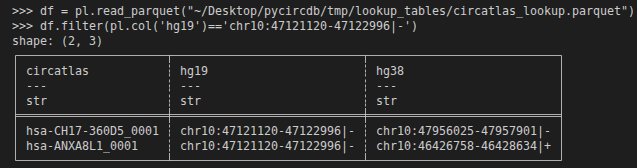
\includegraphics[width=0.8\linewidth]{Chapter4/Figures/Supp_Figure_1a.png}\\
  \small (B)

  \vspace{1em}

  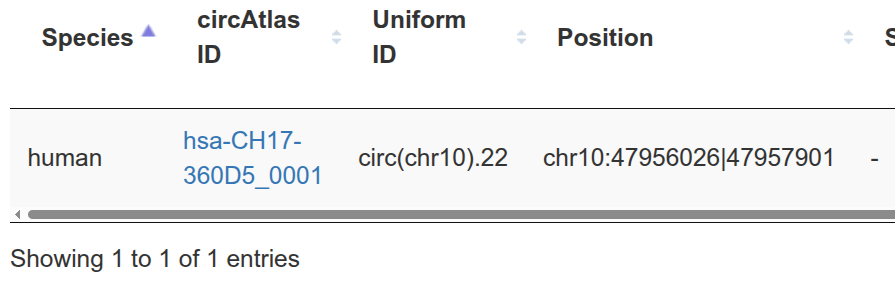
\includegraphics[width=0.8\linewidth]{Chapter4/Figures/Supp_Figure_1b.png}\\
  \small (C)

  \vspace{1em}

  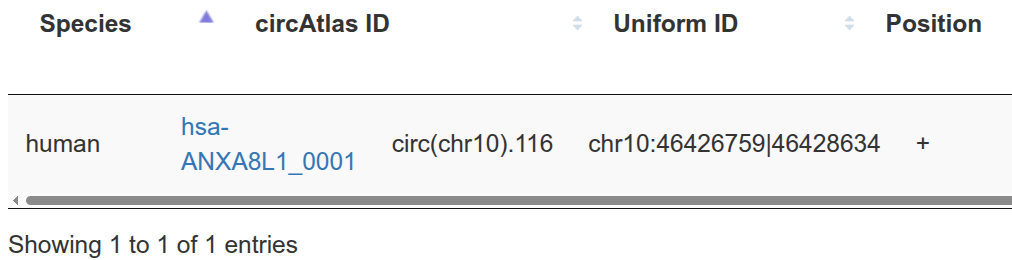
\includegraphics[width=0.8\linewidth]{Chapter4/Figures/Supp_Figure_1c.png}\\
  \small (D)

  \caption[One-to-many hg38 mapping for the hg19 locus chr10:47121120-47122996$|-$]{One-to-many hg38 mapping for the hg19 locus chr10:47121120-47122996$|-$. (A) UCSC liftOver results for the locus. The forward liftover (hg19$\to$hg38) returns a single hg38 coordinate, even with the \texttt{-multiple} flag. However, the reverse liftover (hg38$\to$hg19) shows that two independent hg38 coordinates each map back to the same hg19 coordinate, reflecting a segmental duplication present in hg38 but collapsed in hg19. pycircdb captures this asymmetry by running the reverse lift-over from each hg38-native database entry; both mappings are retained rather than collapsed. Note: UCSC liftOver and circAtlas display coordinates in 1-based convention; pycircdb normalises all coordinates to 0-based. (B) pycircdb lookup table retaining both hg38 mappings under the same hg19 key. (C) circAtlas entry for hsa-CH17-360D5\_0001, confirming the first hg38 mapping (chr10:47956026-47957901$|-$). (D) circAtlas entry for hsa-ANXA8L1\_0001, confirming the second hg38 mapping (chr10:46426759-46428634$|+$).}
  \label{pycircsuppfig1}
\end{figure}

\clearpage

\begin{figure}[ht]
  \centering
  \begin{adjustbox}{width=0.85\paperwidth,center}
    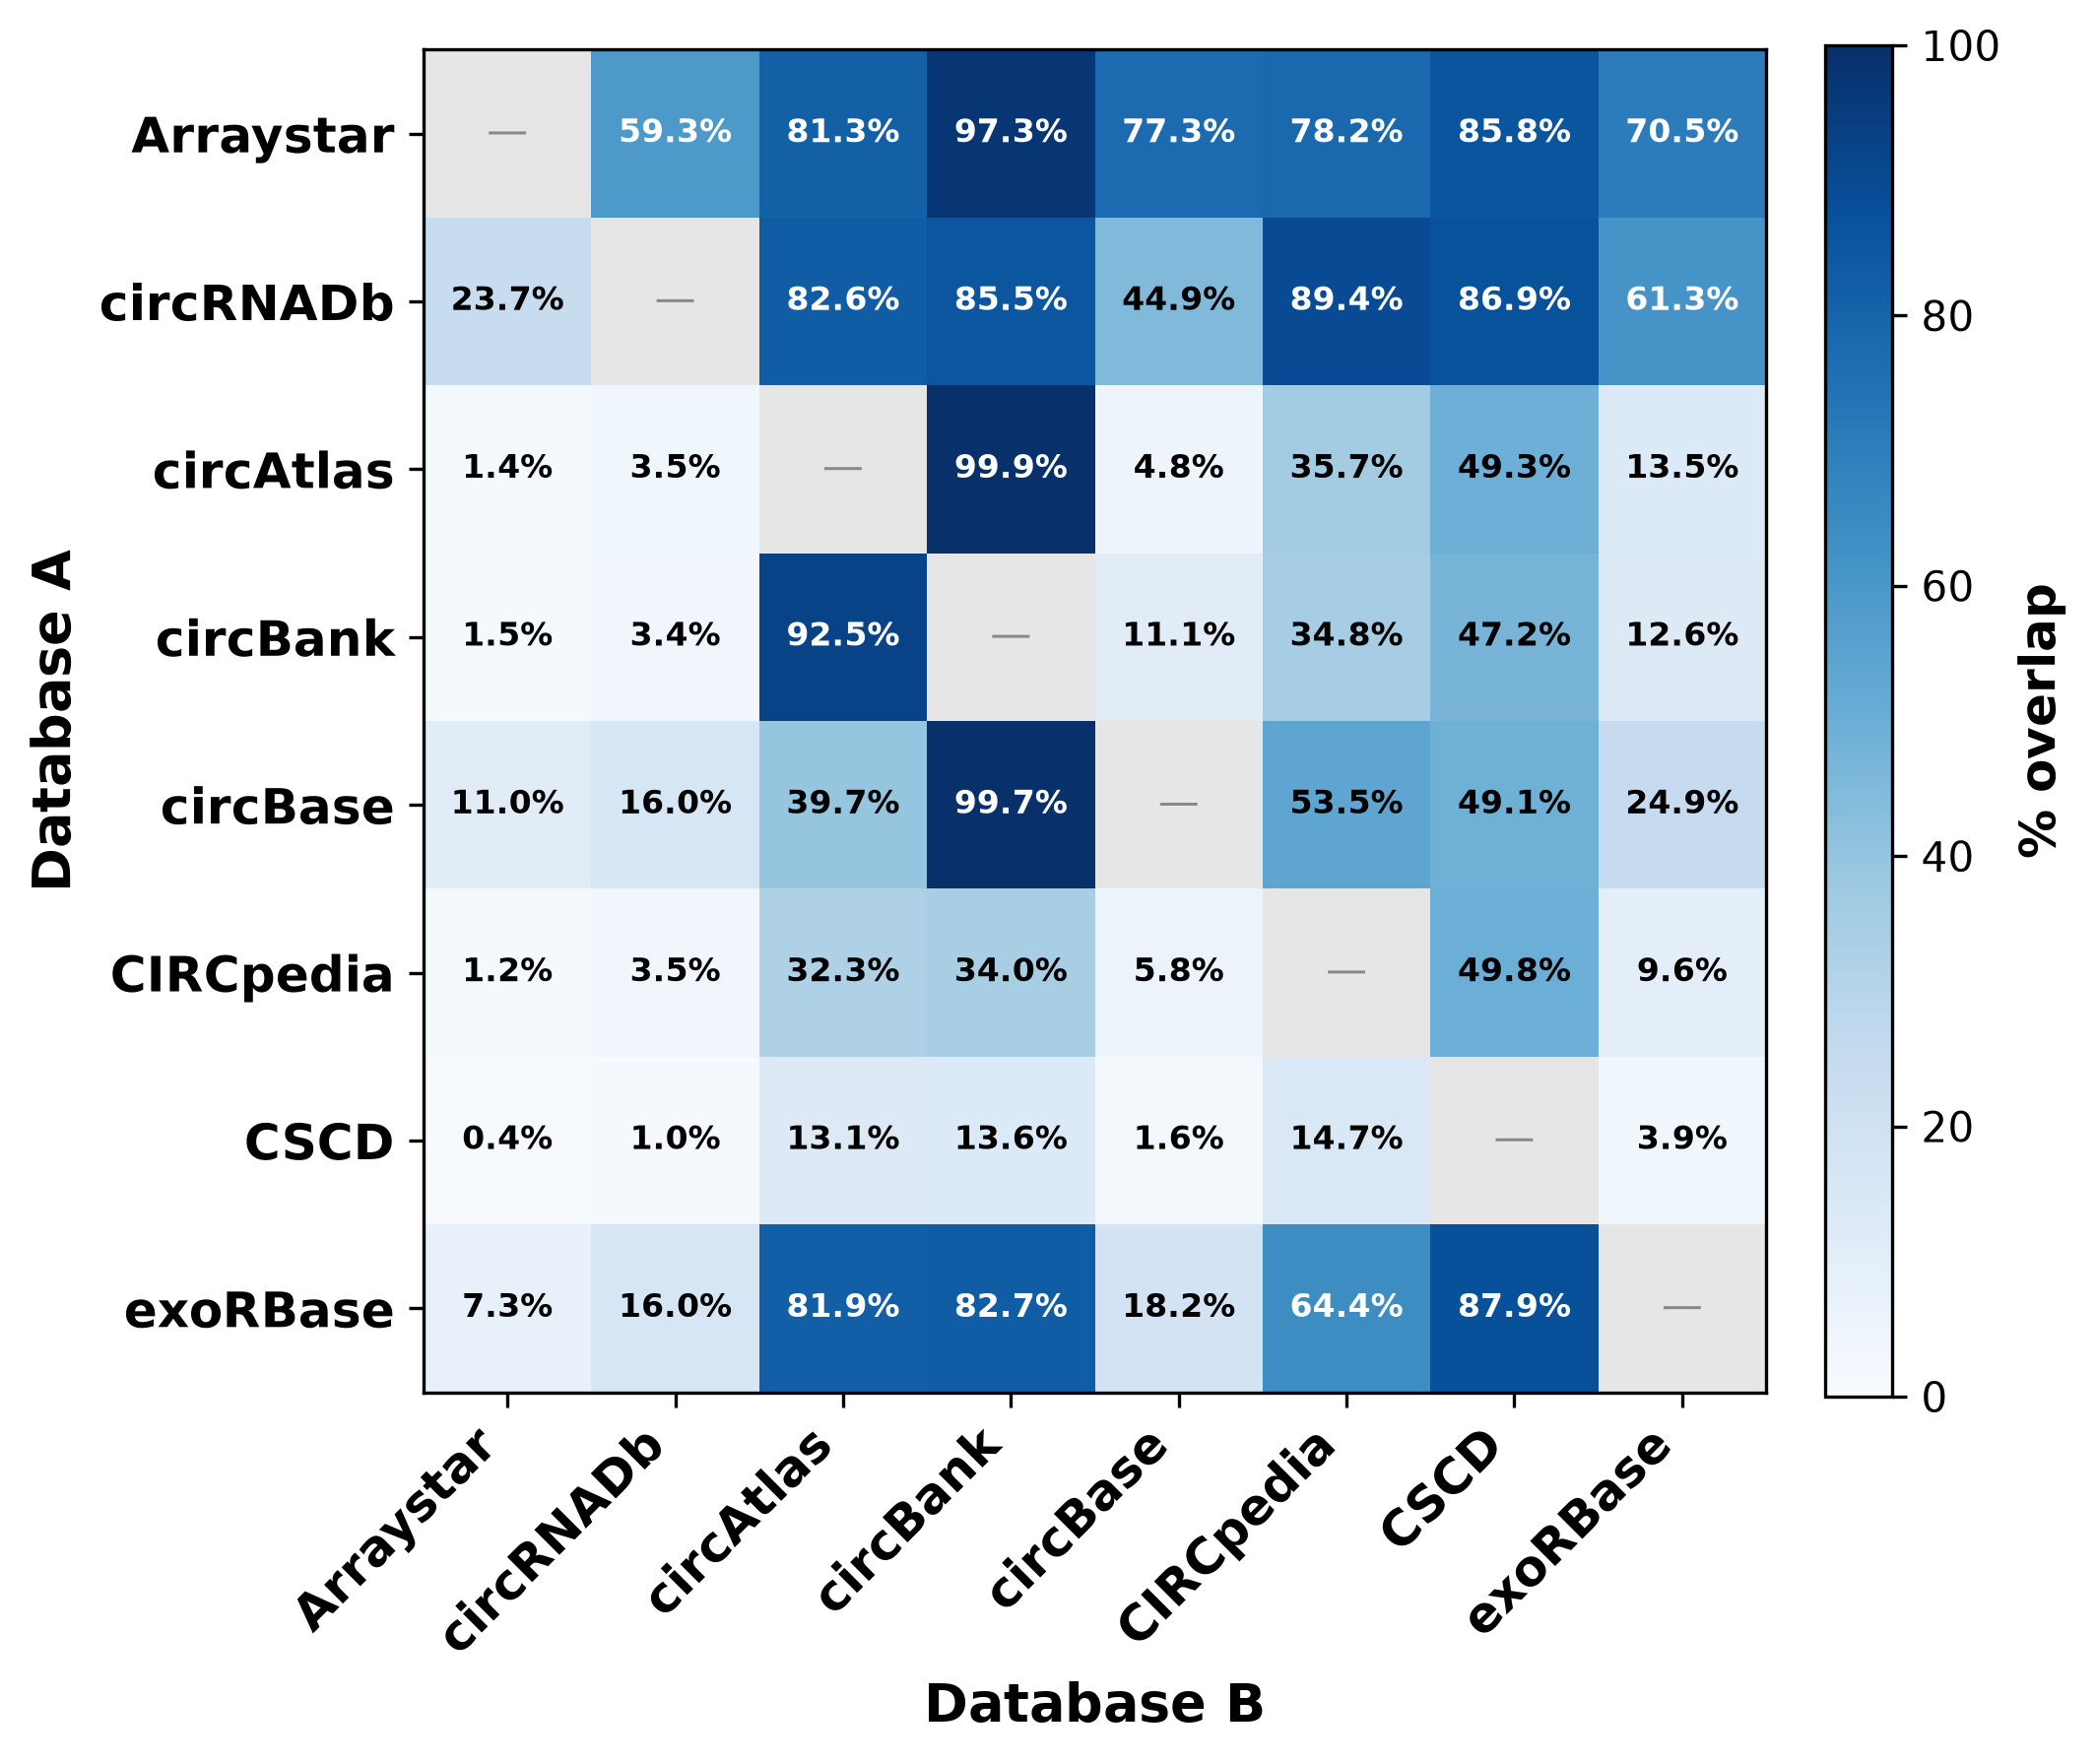
\includegraphics{Chapter4/Figures/Supp_Figure_2.png}
  \end{adjustbox}
  \caption[Pairwise hg19 circRNA overlap between pycircdb lookup tables]{Pairwise hg19 circRNA overlap between pycircdb lookup tables. Each cell gives the percentage of row database A's circRNAs that are also present in column database B.}\label{pycircsuppfig2}
\end{figure}

\clearpage

\begin{figure}[ht]
  \centering
  \begin{adjustbox}{width=0.85\paperwidth,center}
    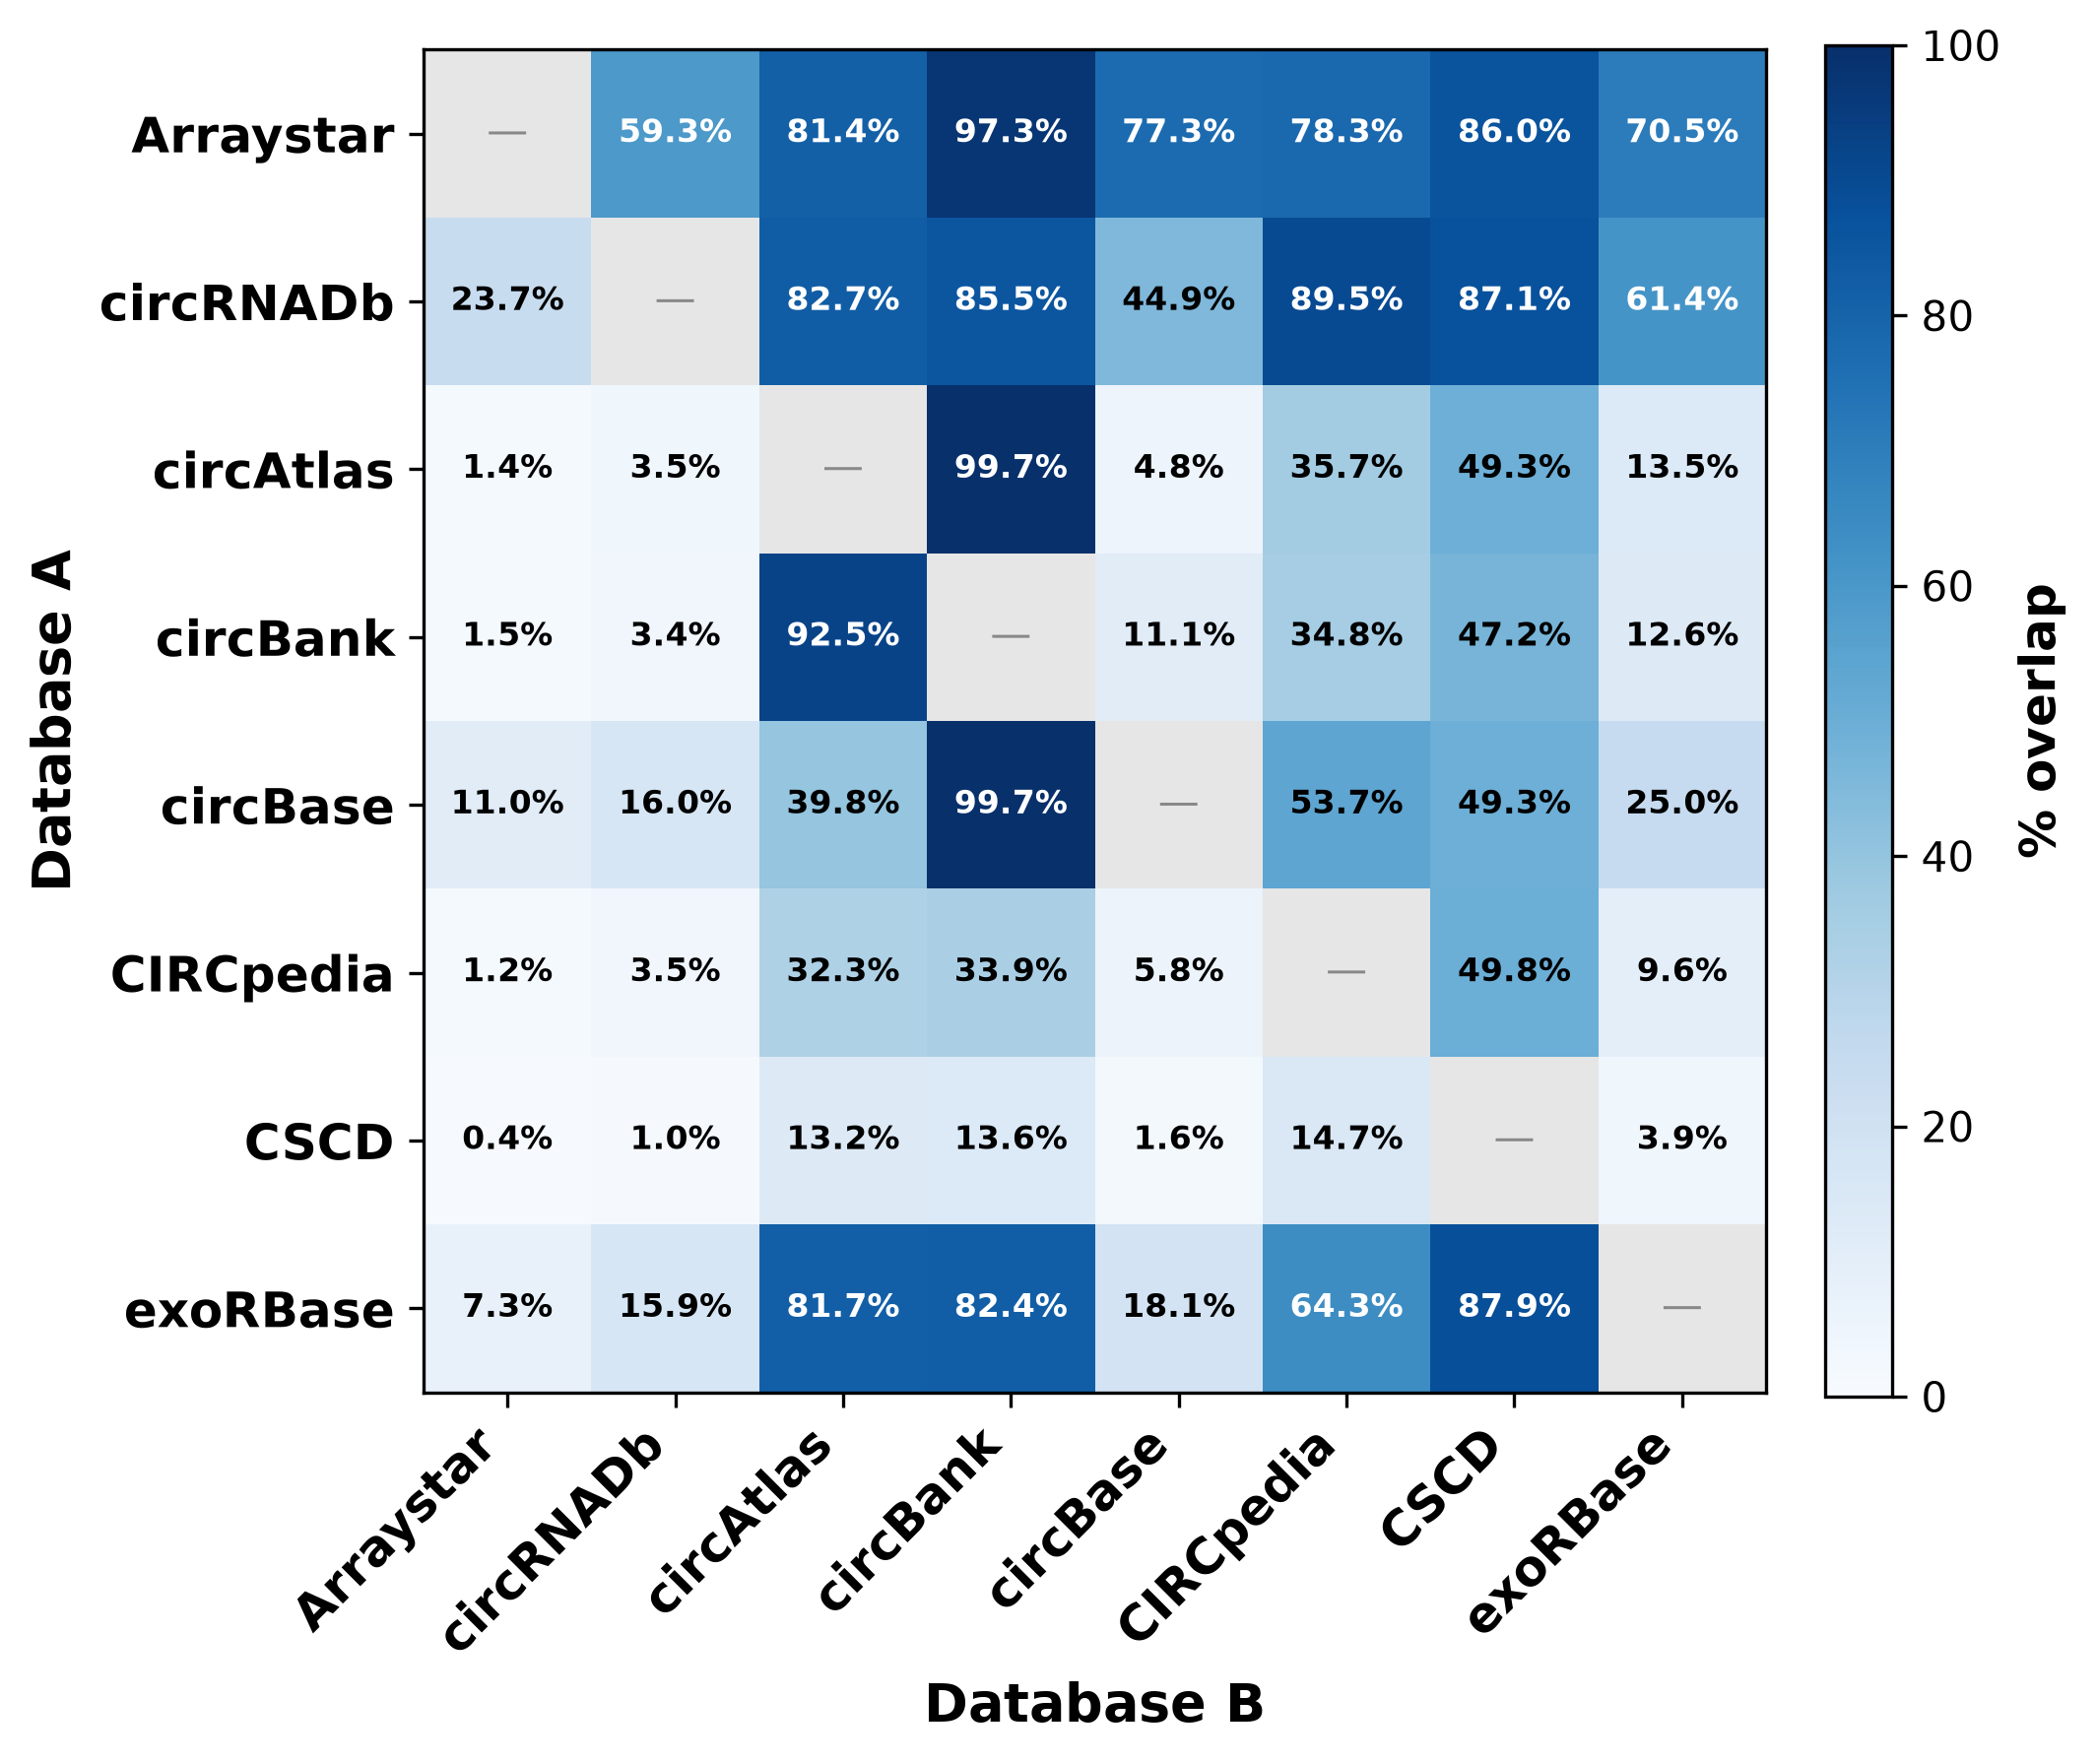
\includegraphics{Chapter4/Figures/Supp_Figure_3.png}
  \end{adjustbox}
  \caption[Pairwise hg38 circRNA overlap between pycircdb lookup tables]{Pairwise hg38 circRNA overlap between pycircdb lookup tables. Each cell gives the percentage of row database A's circRNAs that are also present in column database B.}\label{pycircsuppfig3}
\end{figure}

\clearpage

\begin{figure}[ht]
  \centering
  \begin{adjustbox}{width=0.85\paperwidth,center}
    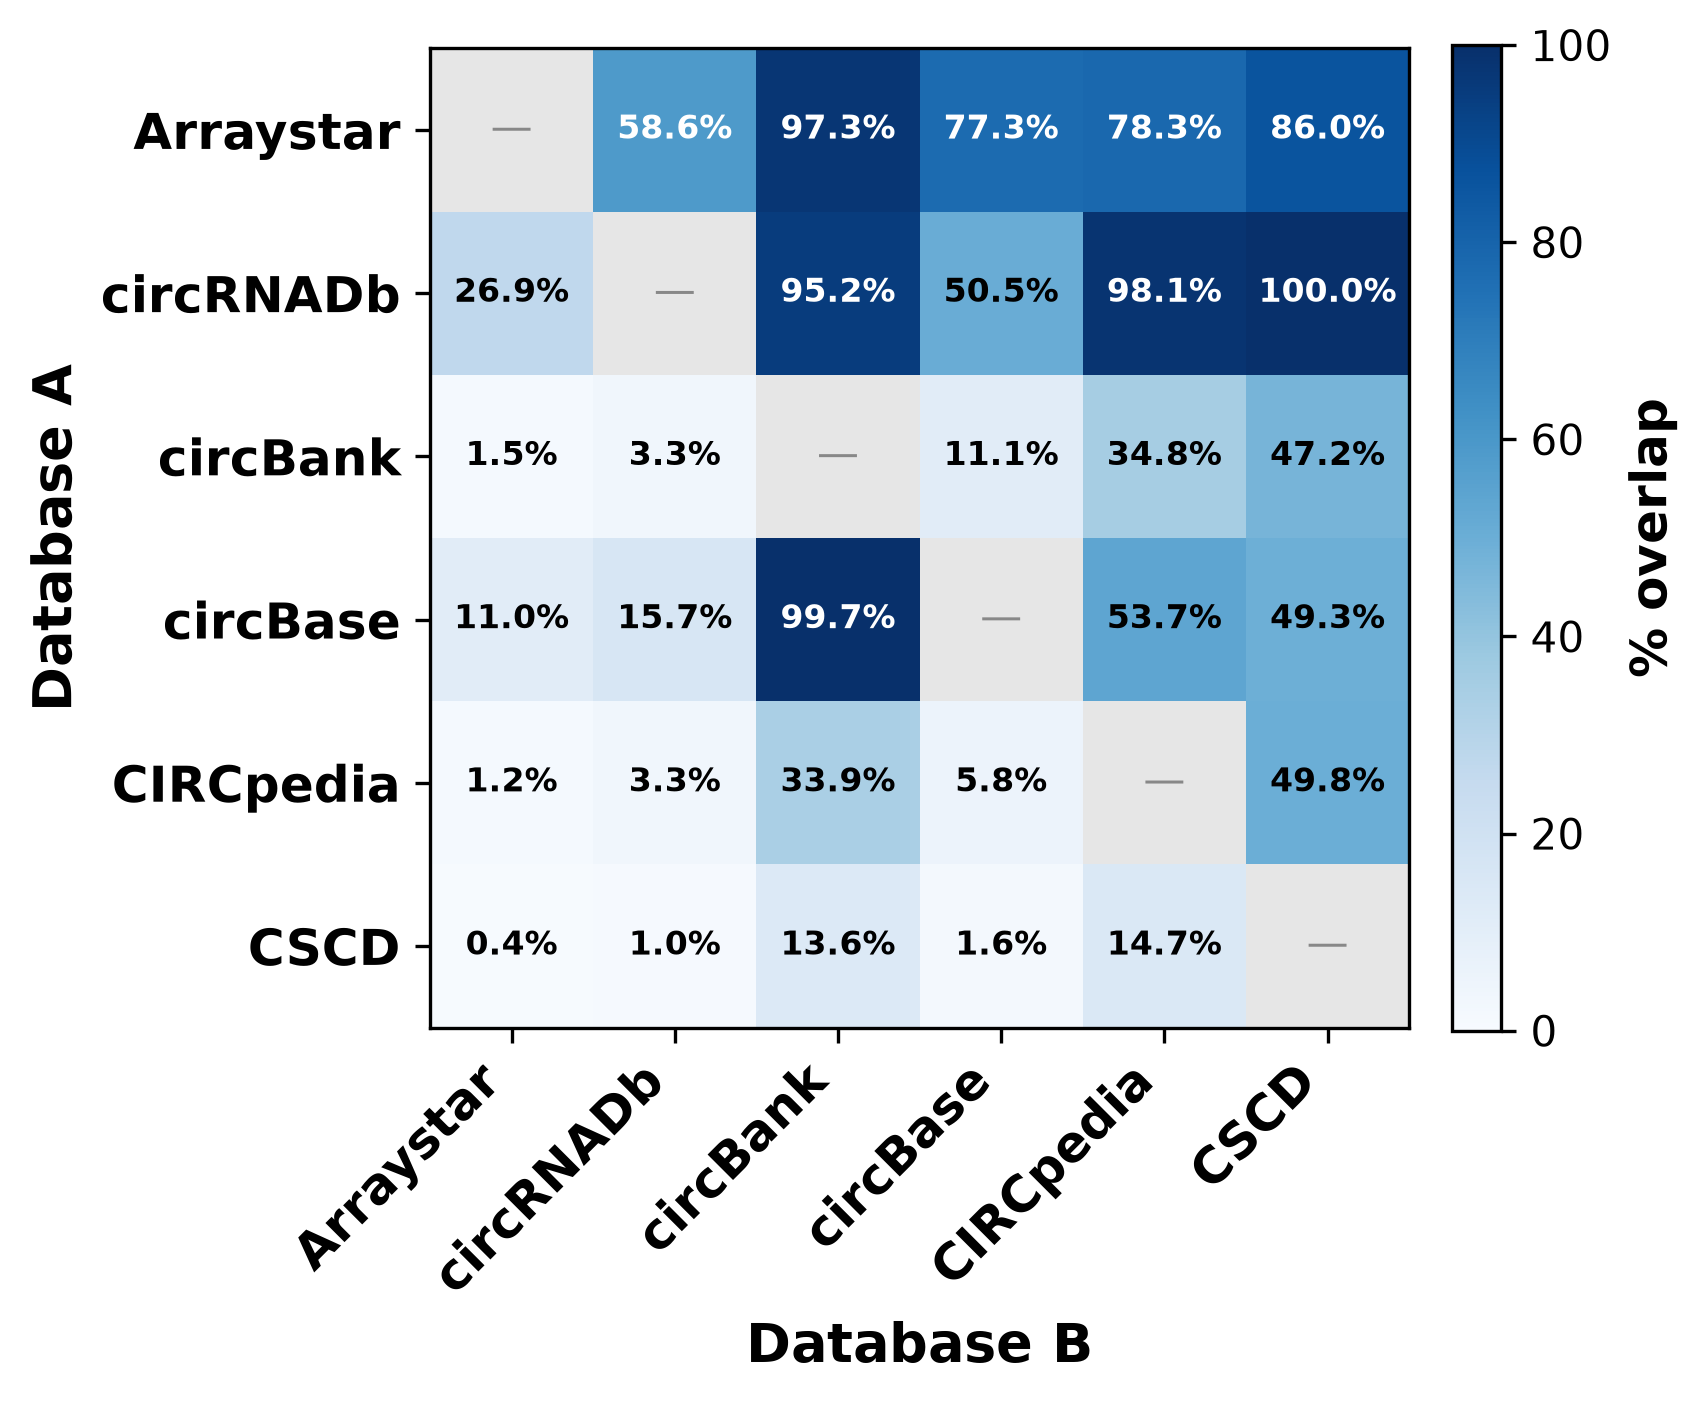
\includegraphics{Chapter4/Figures/Supp_Figure_4.png}
  \end{adjustbox}
  \caption[Pairwise coordinate-level overlap among databases with available FASTA sequences (hg38 coordinates)]{Pairwise coordinate-level overlap among databases with available FASTA sequences (hg38 coordinates). Each cell gives the percentage of row database A's circRNAs that share an hg38 coordinate with column database B. Note: overlap is assessed at the coordinate level, not by sequence identity.}\label{pycircsuppfig4}
\end{figure}

\clearpage


{\Huge \bfseries \noindent Chapter 5}
\vspace{-1em} 
\section*{\LARGE Competing endogenous RNA axis defines a prognostic signature for biochemical recurrence in prostate cancer}
\addcontentsline{toc}{section}{5\quad Competing endogenous RNA axis defines a prognostic signature for biochemical recurrence in prostate cancer}
\setcounter{section}{5}
\setcounter{subsection}{0}  % reset so next \subsection is 2.1
\renewcommand{\chapternum}{5}

% Reset figure/table numbering after chapter 4 supplementary overrides
\renewcommand{\thefigure}{\chapternum.\arabic{figure}}
\setcounter{figure}{0}
\renewcommand{\thetable}{\chapternum.\arabic{table}}
\setcounter{table}{0}


\begin{center}
    \textit{The contents of this chapter are currently under peer review at Scientific Reports}
\end{center}


\subsection*{Abstract}
Androgen deprivation therapy is the mainstay for the treatment of localised prostate cancer, yet one in three patients progress towards a castrate-resistant prostate cancer phenotype. Second-generation anti-androgen drugs such as enzalutamide show overall benefits to survival in castrate-resistant prostate cancer patients; however, patients ultimately acquire resistance to enzalutamide, progressing to metastatic castrate-resistant prostate cancer. In this study, we constructed a circular RNA–micro RNA–messengerRNA competing endogenous RNA network by integrating transcriptomic profiles from enzalutamide-resistant LNCaP cell lines and prostate cancer patients experiencing biochemical recurrence. Messenger RNAs within this shared regulatory network were used to derive a prognostic gene signature across nine independent prostate cancer cohorts with time-to-biochemical recurrence metadata. Model robustness and generalisability were assessed using internal–external cross-validation, bootstrap resampling, validation in an independent external dataset and comparisons to published signatures. We present a 23-gene prognostic signature that predicts biochemical recurrence within five years and is largely distinct from previously published signatures, highlighting the utility of modelling transcriptomic signatures through the lens of regulatory RNA interactions.




\subsection{Introduction}\label{sec1}
Prostate Cancer (PCa) is the second most frequently occurring cancer and the fifth leading cause of cancer-associated deaths in men \cite{Sung2021}. Radical prostatectomy, external beam radiotherapy or brachytherapy are the mainstay of treatment for localised PCa. Approximately 35\% of men experience biochemical recurrence (BCR) after treatments defined by three consecutive rises in prostate-specific antigen (PSA) levels 1 week apart \cite{Rans2022}, progressing to castrate-resistant prostate cancer (CRPC), increasing the risk of distant metastasis and poor survival outcome \cite{Shore2024}. Enzalutamide is a second-generation androgen deprivation therapy drug administered to patients experiencing postoperative recurrence events, competitively binding the androgen receptor (AR), impeding AR signalling and arresting PCa growth \cite{Koochekpour2010}. Despite overall survival benefits of 4.8 months in patients, between 20\%-40\% are intrinsically resistant, whilst all patients will eventually acquire resistance to the drug as measured by increasing PSA levels \cite{Scher2012Sep, Cornford2017}. There is therefore an increasing need to identify biomarkers associated with biochemical recurrence to guide treatment options for PCa patients, improving quality of life and overall survival.

Next-generation sequencing (NGS) provides researchers with a powerful tool to detect biomarkers in clinical samples. The preparation times, sequencing time, and costs associated with NGS technologies are consistently reducing, making NGS a cost-effective tool for biomarker discovery \cite{Lopez2015}. RNA biomarkers are of particular interest, as they provide a snapshot of dynamic cellular states compared to DNA biomarkers and also exhibit superior sensitivity and specificity compared to protein biomarkers \cite{Nimse2016, Xi2017}. The ENCODE project revealed that 76\% of the human genome is transcribed, but only 1.2\% of this represents protein-coding genes \cite{Consortium2012, Djebali2012}, resulting in an increased interest in non-coding RNAs (ncRNAs) and their role in gene regulation. 

Non-coding RNAs (ncRNAs) can be categorised as small ncRNAs ($\le$200nt length) comprising micro RNAs (miRNAs), piwi-interacting RNAs (piRNAs), small nucleolar RNAs (snoRNAs), and long non-coding RNAs (lncRNAs) ($\geq$200nt length). More recently, circular RNAs (circRNAs), originally believed to be aberrant by-products of splicing \cite{Cocquerelle1993Jan, Qian1992}, have emerged as a class of ncRNAs. circRNAs harbour functionally active and evolutionarily conserved miRNA response elements (MRE) within their mature spliced sequence, which are capable of sequestering miRNAs and have been shown to act as competitive endogenous RNAs (ceRNAs) in circRNA-miRNA-mRNA regulatory networks \cite{Thomas2014Aug, Hansen2013Mar, Denzler2014Jun}. Several studies detailing the role of ncRNAs in PCa have since emerged, identifying potential molecular biomarkers and new therapeutic strategies advancing our understanding of disease progression \cite{Aird2018, Bolton2014, Ghiam2017, Ding2021, Takayama2015}.

Recently, several studies have sought to identify prognostic markers by exploring the ceRNA network in diseases \cite{He2022Dec, Song2020Aug, Huang2023Oct, Zhang2023Dec, Guo2020Jul, Shang2025May}. This strategy reduces the input feature space for prognostic modeling by performing differential expression analysis at three levels (circRNA, miRNA, and mRNA), predicting RNA–RNA interactions, and filtering by direction of fold change to construct tri-partite circRNA–miRNA–mRNA graphs that reflect predicted ceRNA network activity. In contrast, traditional approaches that rely on differential expression analysis, dimension reduction, supervised machine learning, or any combination thereof solely at the gene level, may overlook regulatory interactions between RNA biotypes.

Whilst such studies are novel in the sense of incorporating regulatory networks, they are not immune to the common pitfalls of reporting model transparency \cite{Dhiman2021Oct}. Authors typically report the prognostic model's validation in the training dataset and external validation results, which can be severely overoptimistic in studies lacking appropriate power due to overfitting \cite{Steyerberg2015Apr}. Furthermore, authors may neglect to report heterogeneity in model performance across relevant patient groups, thereby omitting information regarding model generalizability \cite{Riley2016Jun}.

In this study, we develop a prognostic model capable of predicting BCR and validate our prognostic model through internal-external cross-validation, bootstrap resampling, optimism-corrected apparent performance, and external validation to ensure transparency in model performance. The code used to perform the analysis is available at \href{https://github.com/BarryDigby/pca_network}{BarryDigby/pca\_network}, facilitating reuse and adaptation to future research.


\subsection{Methods}\label{sec2}

\subsubsection{Data collection}\label{methods1}
Differential expression analysis and subsequent ceRNA network construction were performed using two circRNA datasets, seven miRNA datasets, and five mRNA datasets (Supplementary Table \ref{chp4supptable1}, Supplementary Table \ref{chp4supptable2}, Supplementary File \hyperlink{chp4suppfile1}{1}). Each RNA biotype group included at least one dataset comparing primary PCa to normal tissue, and at least one dataset comparing enzalutamide-resistant to enzalutamide-sensitive samples. Prognostic model development and validation were performed using ten survival PCa datasets containing time to BCR, Gleason score and PSA level metadata (Supplementary Table \ref{chp4supptable3}).

\subsubsection{Data processing}\label{methods2}
Quantile normalized, log2 transformed circRNA, miRNA and mRNA microarray datasets (GSE113153, GSE118959, GSE45604, GSE46738, GSE143408 and GSE78201) were downloaded using GEOquery \cite{Davis2007} and analysed in R (version 4.2.0). GSE21036, GSE23022 and GSE36803 miRNA and mRNA raw CEL files were downloaded from ArrayExpress \cite{Parkinson2007}, RMA normalised, and Log2 transformed using the oligo package \cite{Carvalho2010} prior to differential expression analysis. GSE88752, TCGA-PRAD miRNA and TCGA-PRAD mRNA count data were normalised with respect to library size using edgeR \cite{Robinson2010Jan} and transformed using limma-voom \cite{Law2014Feb}. 

In-house LNCaP small RNA-Sequencing data were processed using custom scripts available on GitHub. Briefly, the reference miRBase hairpin FASTA file was downloaded and converted to DNA sequences using \textit{seqkit seq --rna2dna} before indexing using Bowtie \cite{Bowtie, Shen2016}. Next, raw sequencing reads were subject to adapter removal using the TruSeq smallRNA adapter sequence, clipping 4 bases from the 5' and 3' ends of reads and filtering to remove reads of length $<$17nt or $>$30nt \cite{Krueger2023}. The processed reads were collapsed using \textit{seqcluster collapse} and aligned to the reference hairpin file using Bowtie \cite{Pantano2016, Bowtie}. For each read, 2 mismatches were allowed in the seed region, and the optimal alignment was selected from the 50 reported alignments using \textit{-n 2 -k 50 --best --strata}. Candidate miRNAs were quantified against the miRBase GFF file using \textit{mirtop} with default parameters \cite{Desvignes2020}. In-house LNCaP RNA-Sequencing samples were processed using the `STAR-Salmon' transcript quantification subworkflow in nf-core/rnaseq v3.12.0 \cite{Patel2023}. 

Pre-normalised log2 CPM RDS files were downloaded from PCaDB and used for prognostic model development \cite{Li2022Jan}. Each dataset was centred and scaled, with duplicate gene identifiers collapsed to select the highest variance.

\subsubsection{Identification of co-expressed differentially expressed RNAs}\label{methods3}
Limma \cite{Ritchie2015} was used to identify differentially expressed circRNAs, miRNAs and mRNAs in each respective dataset, with an adjusted \textit{P} value $\leq$0.05 after Benjamini-Hochberg multiple testing correction deemed statistically significant. Co-expressed circRNAs, miRNAs and mRNAs were identified by selecting probes/genes that are present in both PCa vs. normal and enzalutamide-resistant vs. enzalutamide-sensitive limma TopTable results, and exhibit the same fold change direction. Custom scripts were used to convert both Arraystar human circRNA microarray V2 probes to circbase IDs and outdated miRNA probe IDs to their latest miRBase aliases, ensuring standardisation of results and compatibility with downstream target prediction analysis.

\subsubsection{circRNA, miRNA, mRNA target prediction}\label{methods4}
The predicted miRNA targets of screened differentially expressed (DE) circRNAs were obtained using the CircBase database \cite{circbase} and the Cancer-Specific CircRNA Database \cite{CSCD}, generating database-guided circRNA-miRNA pairs. DE-miRNAs were subsetted using the intersection of the predicted circRNA-miRNA targets. Finally, the gene targets of DE-miRNAs were obtained using miRBase \cite{mirbase}, miRTarBase \cite{mirtarbase}, miRNet \cite{mirnet}, and TargetScan \cite{Targetscan}. Predicted miRNA-mRNA targets were intersected with DE-mRNAs to produce a DE-circRNA/DE-miRNA/DE-mRNA tripartite graph of predicted interactions.

\subsubsection{Construction of ceRNA network}\label{methods5}
In addition to identifying circRNA-miRNA and miRNA-mRNA pairs via sequence-specific context, the expression profiles of each pair were incorporated to deduce the final ceRNA network by selecting pairs with opposite fold change direction. The resulting circRNA-miRNA-mRNA tripartite graphs passing filtering exhibited downregulated-upregulated-downregulated and upregulated-downregulated-upregulated expression patterns, respectively.

\subsubsection{Prognostic model development}\label{methods6}
Prognostic model development using DE-mRNAs in the ceRNA network in addition to the clinical covariates Gleason score and PSA, was carried out using a dataset comprising the Belfast, CIT, CMap, CPC, DKFZ, GSE54460, Stockholm, TCGA, and Taylor datasets—henceforth referred to as the derivation dataset. The CoxBoost algorithm was chosen for feature selection with parameters \textit{minstepno} and \textit{maxstepno} set to 5 and 35, respectively, to generate a model with \textit{n} predictors that would satisfy the number of events per predictor ranging from 15-50 \cite{Harrellbook, Ogundimu2016Aug, Wynants2015Dec, Austin2014Nov}. The coefficients of the final model were extracted and used in a multivariate Cox proportional hazards model to assess the Schoenfeld residuals \cite{Schoenfeld1982}; predictors violating the assumptions were removed from the final prognostic model. 

\subsubsection{Prognostic model evaluation}\label{methods7}
\paragraph{Performance in derivation and external validation dataset}\label{methods71}
The discriminative power, overall model fit and predictive accuracy of the prognostic model in the derivation and validation datasets were calculated as detailed in Royston et. al \cite{Royston2013}: 1) The calibration slope in the validation dataset was computed and compared to the slope of the derivation dataset. A calibration slope $<$1 suggests less discriminative power, whilst a slope $>$1 indicates superior discriminative power in the validation dataset. 2) The overall fit of the prognostic model in the validation dataset was computed via a joint test of all predictors whilst constraining the prognostic index to 1. A small Chi-squared test value and a non-significant \textit{P} value indicate a good fit of the prognostic index in the validation dataset. 3) Harrell's C-index was computed for both the derivation and validation datasets; agreement between the two datasets being indicative of similar predictive performance. 4) Kaplan-Meier survival curves between risk group strata, as defined by the median prognostic index value, were plotted in conjunction with the log-rank \textit{P} value to provide empirical evidence of discrimination. 5) Hazard ratios for the high-risk groups were computed in the validation and derivation datasets. Ideally, the hazard ratio in the derivation dataset should be well maintained in the validation dataset and remain statistically significant. 6) ROC analysis revealed the overall predictive accuracy of the model via AUC. 

\paragraph{Optimism-corrected performance using bootstrap}\label{methods72}
Model optimism was estimated following the procedure described by Harrell et al. \cite{Harrell1996Feb}. 1) A model was fitted to the full derivation dataset to calculate the apparent discrimination $(c_{\text{app}})$. 2) Two hundred bootstrap samples ($M=200$) were generated using resampling with replacement from the derivation dataset. 3) For each bootstrap sample $(m=1, \ldots, M)$, predictor selection and model fitting were performed using the same approach as in step 1 to generate a bootstrap model. The model was then applied to its corresponding bootstrap sample to calculate discrimination $(c_{\text{boot}}^{\phantom{(}}(m))$. 4) For each bootstrap model, discrimination on the original derivation dataset $(c_{\text{orig}}^{\phantom{(}}(m))$ was also calculated. Coefficients from step 3 were fixed to estimate the degree of overfitting due to variable selection. 5) For each iteration, model optimism was calculated as $o^{\phantom{(}}(m) = c_{\text{orig}}^{\phantom{(}}(m) - c_{\text{boot}}^{\phantom{(}}(m)$. The average optimism across all bootstrap samples was computed to obtain the overall optimism of the original model. 6) Finally, the optimism-corrected performance of the model was reported as $c_{\text{adj}} = c_{\text{app}} - o$, providing an estimate of the expected discrimination in external validation.


\paragraph{Internal-external cross-validation}\label{methods8}
To further assess the generalizability of our model, we conducted internal-external cross-validation across the nine studies in the derivation dataset. In each iteration, one study was held out as an independent validation set, while the model was trained using the remaining studies. Importantly, the model coefficients were fixed after training on each combination of development studies and were then directly applied to the held-out dataset, without any refitting or recalibration. This ensures that performance metrics reflect true external validation, avoiding optimistic bias from adapting the model to each test set. Model discrimination was evaluated in each dataset using the steps described in section \ref{methods71}. Calibration slope and Harrell's C-index metrics were pooled across all folds using random-effects meta-analysis to provide an overall summary of performance and an estimate of model heterogeneity.

\paragraph{Comparison to published signatures}\label{methods9}
30 published PCa prognostic signatures (Supplementary Table \ref{chp4supptable4}) were collected and used to create multivariate Cox proportional hazards models representative of each signature. Each signature's performance was assessed as described in section \ref{methods71} using the external validation dataset and compared to our prognostic model derived using a ceRNA network. Coefficients for the published PCa signatures were largely unavailable; thus, comparisons between each model is based on feature selection alone and does not include analysis of coefficient estimation. Notably, the published signatures did not include any clinical covariates.


\subsection{Results}
\subsubsection{Identification of ceRNA network}\label{results1}
The contrasts used in the DE analysis of each RNA dataset and the summary of their results are provided in Table \ref{table1}. Differential circRNA expression analysis revealed 232 DE-circRNAs (168 up-regulated, 64 down-regulated). Target prediction of DE-circRNAs was performed using the CircBase and CSCD databases, returning 30,727 predicted circRNA-miRNA pairs. The intersection of the 30,727 predicted circRNA-miRNA interactions with 42 DE-miRNAs (16 up-regulated, 26 down-regulated) yielded a final set of 42 DE-miRNAs. TargetScan, miRNet, miRTarBase, and miRBase returned 61,193 miRNA-mRNA target predictions based on the 42 input DE-miRNAs. Predictions were intersected using 1,310 DE-mRNAs returned by differential gene expression analysis (691 up-regulated, 619 down-regulated), resulting in a set of 1,090 DE-mRNAs. The preliminary ceRNA network consisting of 232 circRNAs, 42 miRNAs, and 1,090 mRNAs was filtered based on the ceRNA hypothesis --- circRNA-miRNA and miRNA-mRNA pairs were filtered to include pairs exhibiting inverse expression as determined by log fold change sign --- to generate a ceRNA network consisting of 124 circRNAs, 38 miRNAs, and 817 mRNAs. The ceRNA network, including logFC values, is available in the Supplementary\_3.csv file.


\subsubsection{Prognostic model development}
The 817 DE-mRNAs identified in the ceRNA network were used to derive a model predictive of BCR in PCa. 679 DE-mRNAs were present in the derivation dataset, which in combination with the clinical covariates Gleason score and PSA, resulted in 681 predictors used as input to the Coxboost algorithm. 26 non-zero coefficients were returned by the model, with 3 predictors removed for violating proportional hazards assumptions. The 23-gene signature is presented with exponentiated coefficients, confidence intervals and \textit{P} values in Figure \ref{Figure1}A. \par


\begin{table*}[ht!]
\caption[Differentially expressed RNA biotypes]{\textbf{Differentially expressed RNA biotypes} returned by Limma and unique overlapping RNAs with the same fold change direction.\label{table1}}

\begin{adjustwidth}{-0.0in}{-0.0in}
\tabcolsep=0pt%%
\footnotesize
\resizebox{\textwidth}{!}{
\begin{tabular*}{\textwidth}{@{\extracolsep{\fill}}lllrr@{\extracolsep{\fill}}}
\toprule
\textbf{Data type} & \textbf{Series} & \textbf{Contrast} & \textbf{DE-up} & \textbf{DE-down} \\
\midrule
  circRNA & GSE113153 & Gleason high vs. low & 2,608 & 1,979
  \\
  circRNA & GSE118959 & Clone 1 vs. control & 591 & 729 
  \\ 
  circRNA & GSE118959 & Clone 9 vs. control & 20 & 74
  \\ 
  \midrule
  & & Unique overlapping circRNAs: & 168 & 64
  \\
  \midrule
  miRNA & GSE21036 & Tumor vs. normal & 153 & 145
  \\ 
  miRNA & GSE23022 & Tumor vs. normal & 17 & 8 
  \\ 
  miRNA & GSE36803 & Tumor vs. normal & 36 & 92
  \\ 
  miRNA & GSE45604 & Tumor vs. normal & 22 & 67 
  \\
  miRNA & GSE46738 & Tumor vs. normal & 68 & 68
  \\
  miRNA & GSE312115 & Clone 1 vs. control & 146 & 110 
  \\ 
  miRNA & GSE312115 & Clone 9 vs. control & 4 & 1
  \\
  miRNA & TCGA-PRAD & Tumor vs. normal & 130 & 128
  \\
  \midrule
  & & Unique overlapping miRNAs: & 16 & 26
  \\
  \midrule 
  mRNA & GSE143408 & 7 days ENZ treated vs. 0 days & 3,829 & 3,458
  \\
  mRNA & GSE143408 & 14 days ENZ treated vs. 0 days & 5,693 & 4,792
  \\
  mRNA & GSE143408 & 21 days ENZ treated vs. 0 days & 6,128 & 4,977
  \\
  mRNA & GSE78201 & 6 months ENZ treated vs. control & 518 & 571
  \\
  mRNA & GSE88752 & ENZ-resistant vs. ENZ-sensitive & 3,564 & 2,942
  \\
  mRNA & LNCaP & Clone 1 vs. control & 4,686 & 4,379 
  \\
  mRNA & LNCaP & Clone 9 vs. control & 1,420 & 1,303
  \\
  mRNA & TCGA-PRAD & Tumor vs. normal & 3,860 & 4,506 
  \\
  \midrule
  & & Unique overlapping mRNAs: & 691 & 619 
  \\
\bottomrule
\end{tabular*}}
\end{adjustwidth}
\begin{tablenotes}%
\item[] DE: Differential Expression. Clone 1: Highly enzalutamide-resistant LNCaP cell lines. Clone 9: Moderately enzalutamide-resistant LNCaP cell lines. ENZ: enzalutamide
\end{tablenotes}
\end{table*}


\subsubsection{Evaluation of the prognostic model}
\paragraph{Derivation dataset}
Model performance in the derivation dataset demonstrated good prognostic value. The prognostic index stratified patients into high- and low-risk groups, showing clear and significant separation in Kaplan–Meier survival curves (log-rank test \textit{P} $<$ 0.0001; Figure \ref{Figure1}B). Cox proportional hazards regression analysis was performed to assess the effect size of the high-risk group, revealing a significant association with BCR outcome (HR = 1.385, 95\% CI = 1.15–1.62, \textit{P} = 4.29e-31; Table \ref{table2}). Time-dependent ROC analysis at 1, 3, and 5 years showed consistent AUCs of 0.75, reflecting stable discriminatory performance (Figure \ref{Figure1}C). Furthermore, a Harrell’s C-index of 0.73 in the derivation dataset indicates reasonable discriminative ability for predicting time to BCR (Table \ref{table2}). 

Calibration curve analysis at 1, 3, and 5 years (Supplementary Figure \ref{chp4suppfigure1}) revealed systematic deviations between predicted and observed risk. Across all time horizons, calibration curves lie below the optimal line for lower predicted probabilities, indicating initial overestimation of absolute risk before crossing above the optimal line at higher predicted probabilities, reflecting underestimation in higher-risk patients.


\paragraph{Bootstrap validation}
To assess the stability of genes in our prognostic model, we examined the frequency with which each gene was selected using the CoxBoost algorithm across 200 bootstrap samples using resampling with replacement in the derivation dataset. The top-ranking genes included RNASEH2C (105), SSTR1 (102), and SPARC (94), indicating consistent inclusion across resampled datasets. Several other genes such as BGN (84), LIX1 (68), and NEU3 (60) were also frequently selected. In contrast, features like MAPK8IP2 (21) and B4GALT1 (16) were less stable. These results highlight a core subset of genes with robust selection frequencies, supporting their potential relevance to the prognostic signal. Notably, Gleason score was the most frequently selected feature during bootstrap sampling (118), yet it was not retained during model development on the original derivation dataset. A full table of gene frequencies over the 200 bootstrap iterations is available in Supplementary Table \ref{chp4supptable5}. 
\par
Next, we assessed model performance using the optimism-corrected Harrell’s C index as described in section \ref{methods71} to account for potential overfitting. Averaging $o^{\phantom{(}}(m) = c_{\text{orig}}^{\phantom{(}}(m) - c_{\text{boot}}^{\phantom{(}}(m)$ across all bootstrap samples yielded a mean optimism of 0.04725. Subtracting this optimism from the model’s apparent Harrell’s C index of 0.7291 on the full derivation dataset produced an optimism-corrected Harrell’s C index of 0.6818. This adjusted value provides a more realistic estimate of the model’s predictive discrimination when applied to new, unseen data.

\paragraph{Internal-external cross-validation}
Overall, the prognostic model was sensitive to the effects of heterogeneity between studies in the derivation dataset. The calibration slope for external validation using the Belfast dataset was 2.28, and as low as 1.19 in the CMap dataset (Figure \ref{Figure2}). This is reflected in the calibration slope pooled estimate confidence intervals (1.61, 95\% CI=1.35-1.86). Furthermore, an $I^2$ value of 43.3\% indicates moderate heterogeneity, suggesting that a proportion of the variability in calibration slopes is attributable to differences between studies rather than sampling error.

\par

Although Harrell's C-index values varied across validation datasets (range: 0.68–0.84), the random-effects meta-analysis yielded an $I^2$ of 0.0\%, $\tau^2 = 0$, and \textit{P} = 0.89, indicating no statistical significance in between-study heterogeneity. This likely reflects the wide confidence intervals and limited number of studies, which reduces the power to detect true differences. As such, visual and numerical differences in discrimination performance across studies should still be considered when assessing model transportability. The full table displaying summary statistics for internal-external cross-validation is available in Supplementary Table \ref{chp4supptable6}.

\par

To further explore heterogeneity at the predictor level, gene-specific random slope variances were estimated using mixed-effects Cox models incorporating study as a random effect \cite{Therneau2024Aug}. The majority of genes demonstrated low variance in effect estimates across studies, indicating stable prognostic associations (Supplementary Table \ref{chp4supptable7}). However, a subset of genes exhibited moderate to high random slope variances, highlighting potential heterogeneity in their effect sizes between cohorts. For example, genes PHYHD1, LIX1, MTERF4, and SPARC showed elevated variance estimates (up to 0.13), suggesting variable influence on outcome depending on study context. Overall, 18 of 23 genes exhibit low variance, indicating the model can be generalised to unseen datasets. 


\begin{figure*}[!t]%
\centering
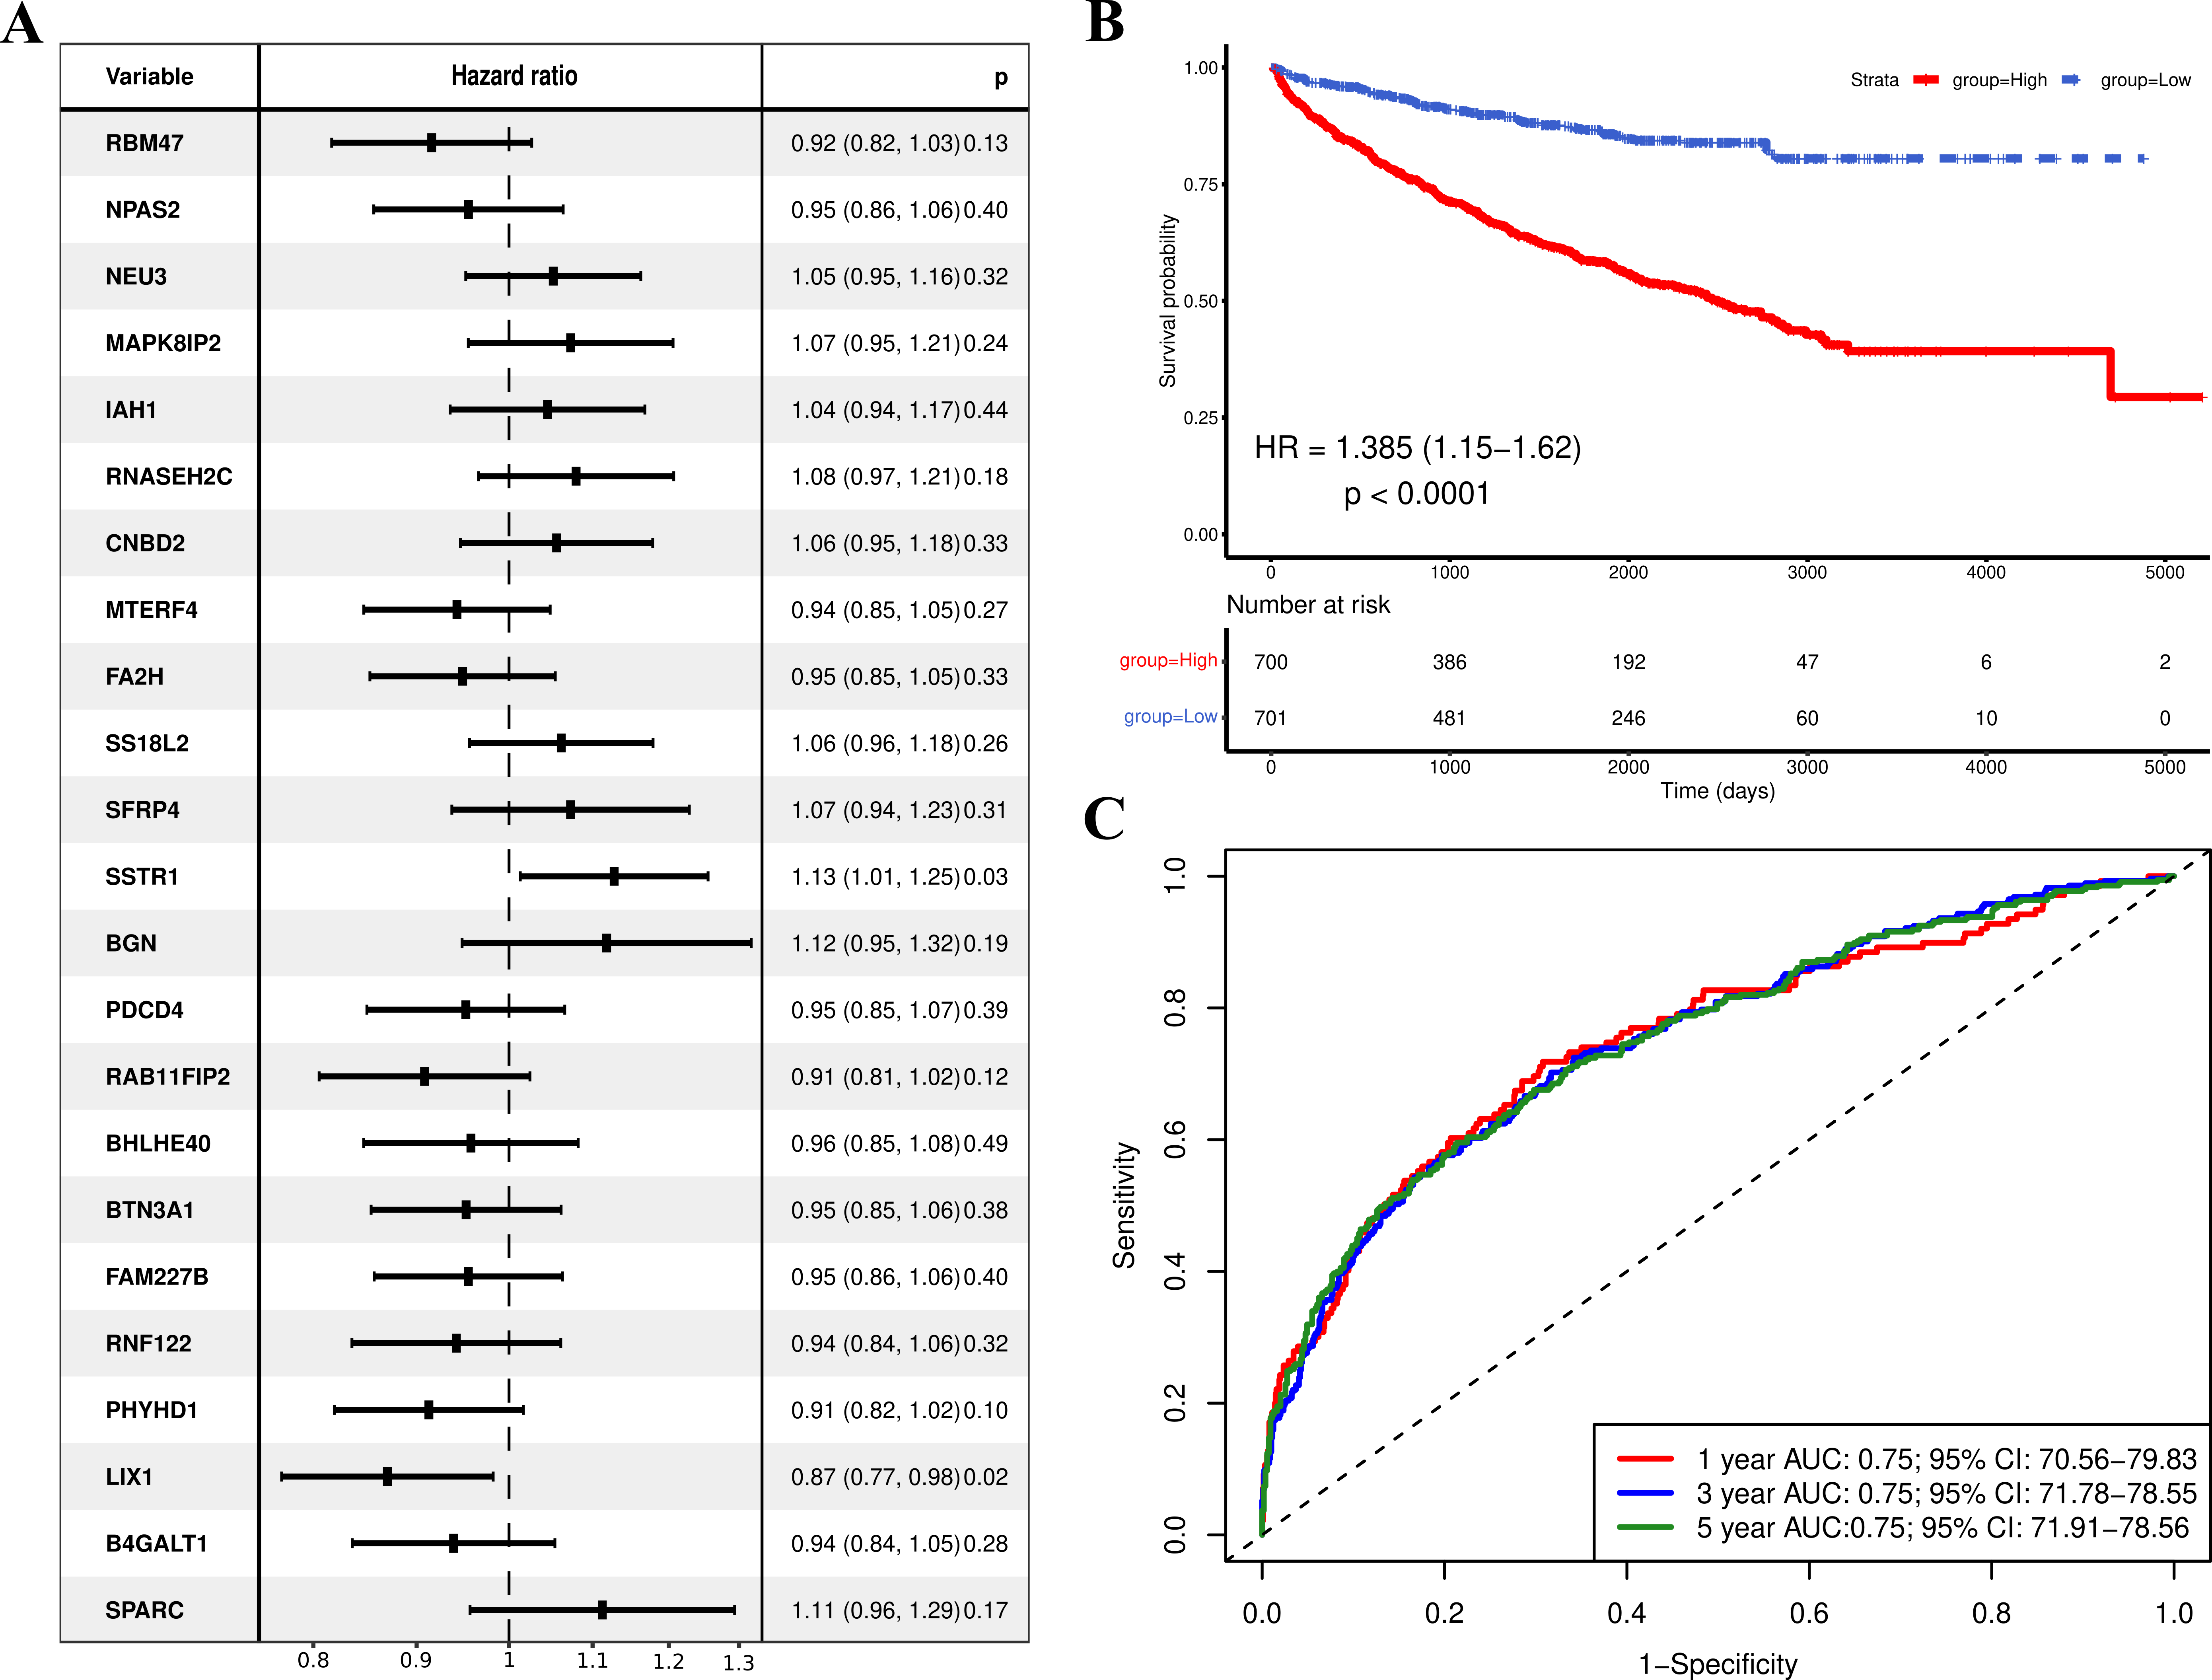
\includegraphics[width=1\textwidth]{Chapter3/Figures/Figure_1.png}
\caption[Prognostic modelling plots]{\textbf{Prognostic modelling plots} (a) Forest plot of non-zero coefficients passing Schoenfeld residual testing returned by Coxboost in the derivation dataset.  (b) Kaplan-Meier plot in the derivation dataset stratified by high-risk (red) and low-risk (blue) groups as defined by the median prognostic index cutoff point. Log-rank \textit{P} value and effect size derived from comparing high-risk to low-risk groups. (c) ROC analysis and AUC prediction accuracy of the prognostic index in the derivation dataset}\label{Figure1}
\end{figure*}

\begin{figure*}[!t]%
\centering
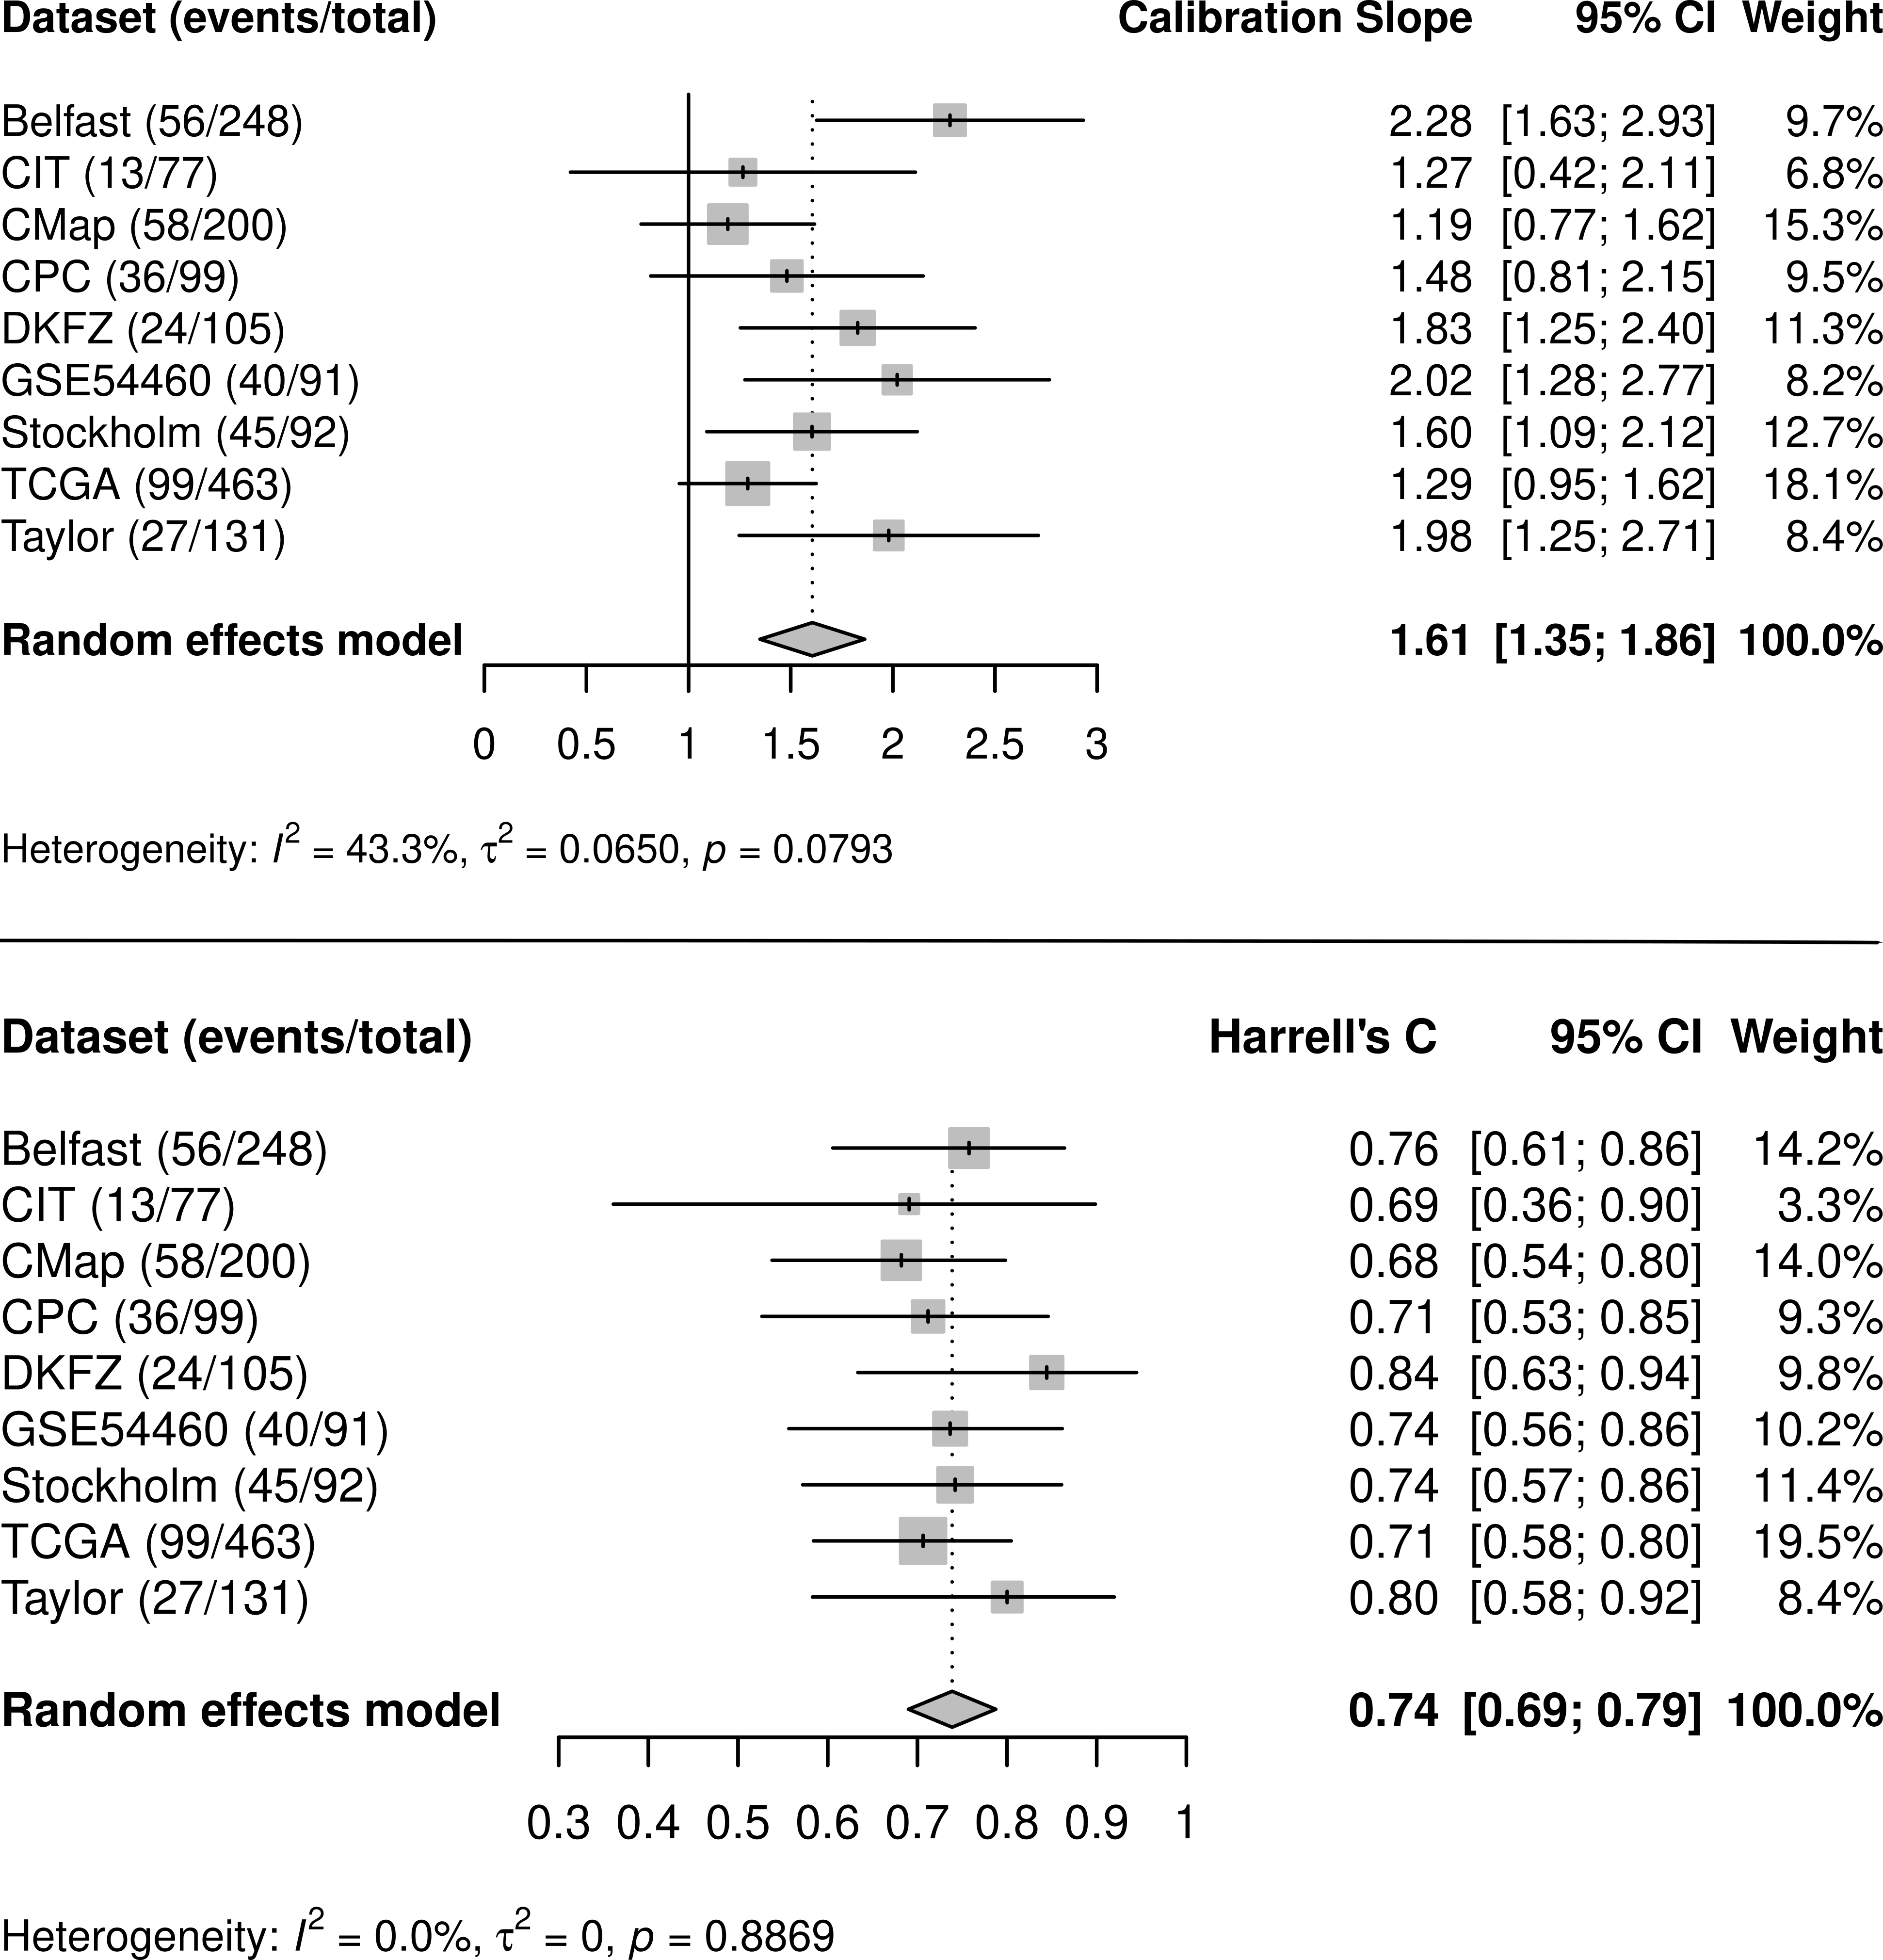
\includegraphics[width=1\textwidth]{Chapter3/Figures/Figure_2.png}
  \caption[Calibration slope, Harrell's C index forest plots]{Results from internal-external cross-validation of Cox proportional hazards model for the calibration slope (top) and Harrell's C index (bottom). Plots display each dataset's performance metric estimates and 95\% confidence intervals (squares with lines), and an overall pooled estimate obtained using random effects meta-analysis and 95\% confidence interval (diamond width encapsulates CI intervals). CI=confidence interval}\label{Figure2}
\end{figure*}

\paragraph{External Validation}
Model performance in the validation dataset remained robust, supporting the portability of the ceRNA network-derived prognostic model. The calibration slope was 1.33 (95\% CI = 0.59–2.06), which, although lower than in the derivation dataset, exceeds 1, indicating a tendency toward underfitting rather than overfitting and adequate predictive reliability (Table \ref{table2}). Discrimination was also well maintained, with time-dependent AUCs of 0.67, 0.78, and 0.87 at 1, 3, and 5 years, respectively (Figure \ref{Figure3}B), and a Harrell’s C-index of 0.71 (Table \ref{table2}). The hazard ratio in the validation cohort was 1.48, consistent with that observed during model development (Figure \ref{Figure3}A, Table \ref{table2}). Although calibration slope and hazard ratio estimates achieved statistical significance, the associated confidence intervals were wide, likely a consequence of the limited sample size in the GSE46602 validation cohort (22 BCR events among 36 patients).


%% use this setup for wide tables throughout thesis, caption + tablenotes nicely aligned. 
\begin{table*}[ht!]
\caption[Evaluation of the prognostic model in the derivation dataset and external validation dataset]{\textbf{Evaluation of the prognostic model in the derivation dataset and external validation dataset}.\label{table2}}
\begin{adjustwidth}{-0.7in}{-0in}
\tabcolsep=0pt%%
\footnotesize
\resizebox{1.2\textwidth}{!}{
\begin{tabular*}{\linewidth}{@{\extracolsep{\fill}}llllllllll@{\extracolsep{\fill}}}
  & \multicolumn{3}{c}{\textbf{Calibration slope}} & \multicolumn{2}{c}{\textbf{Chi-squared}} & & \multicolumn{3}{c}{\textbf{High risk stratum}} \\
  \cline{2-4}\cline{5-6}\cline{8-10} 
  & \textbf{coef} & \textbf{(95\% CI)} & \textbf{\textit{P} value} & \textbf{\(\chi^2_5\)} & \textbf{\textit{P} value} & \textbf{C-index}$^{1}$ & \textbf{Hazard ratio} & \textbf{(95\% CI)} & \textbf{\textit{P} value}
  \\
  \toprule
  Derivation & 1.59 & (1.41, 1.77) & 2.02e-68 & 0 & 1 & 0.73 & 1.38 & (1.15, 1.62) & 4.29e-31
  \\
  Validation & 1.33 & (0.59, 2.06) & 0.00038 & 0 & 1 & 0.71 & 1.48 & (0.52, 2.44) & 0.00257 
  \\
  \toprule
\end{tabular*}}
\end{adjustwidth}
\begin{tablenotes}
\item[$^{1}$] Harrell's C-index
\end{tablenotes}
\end{table*}


\begin{figure}[!h]%
\centering
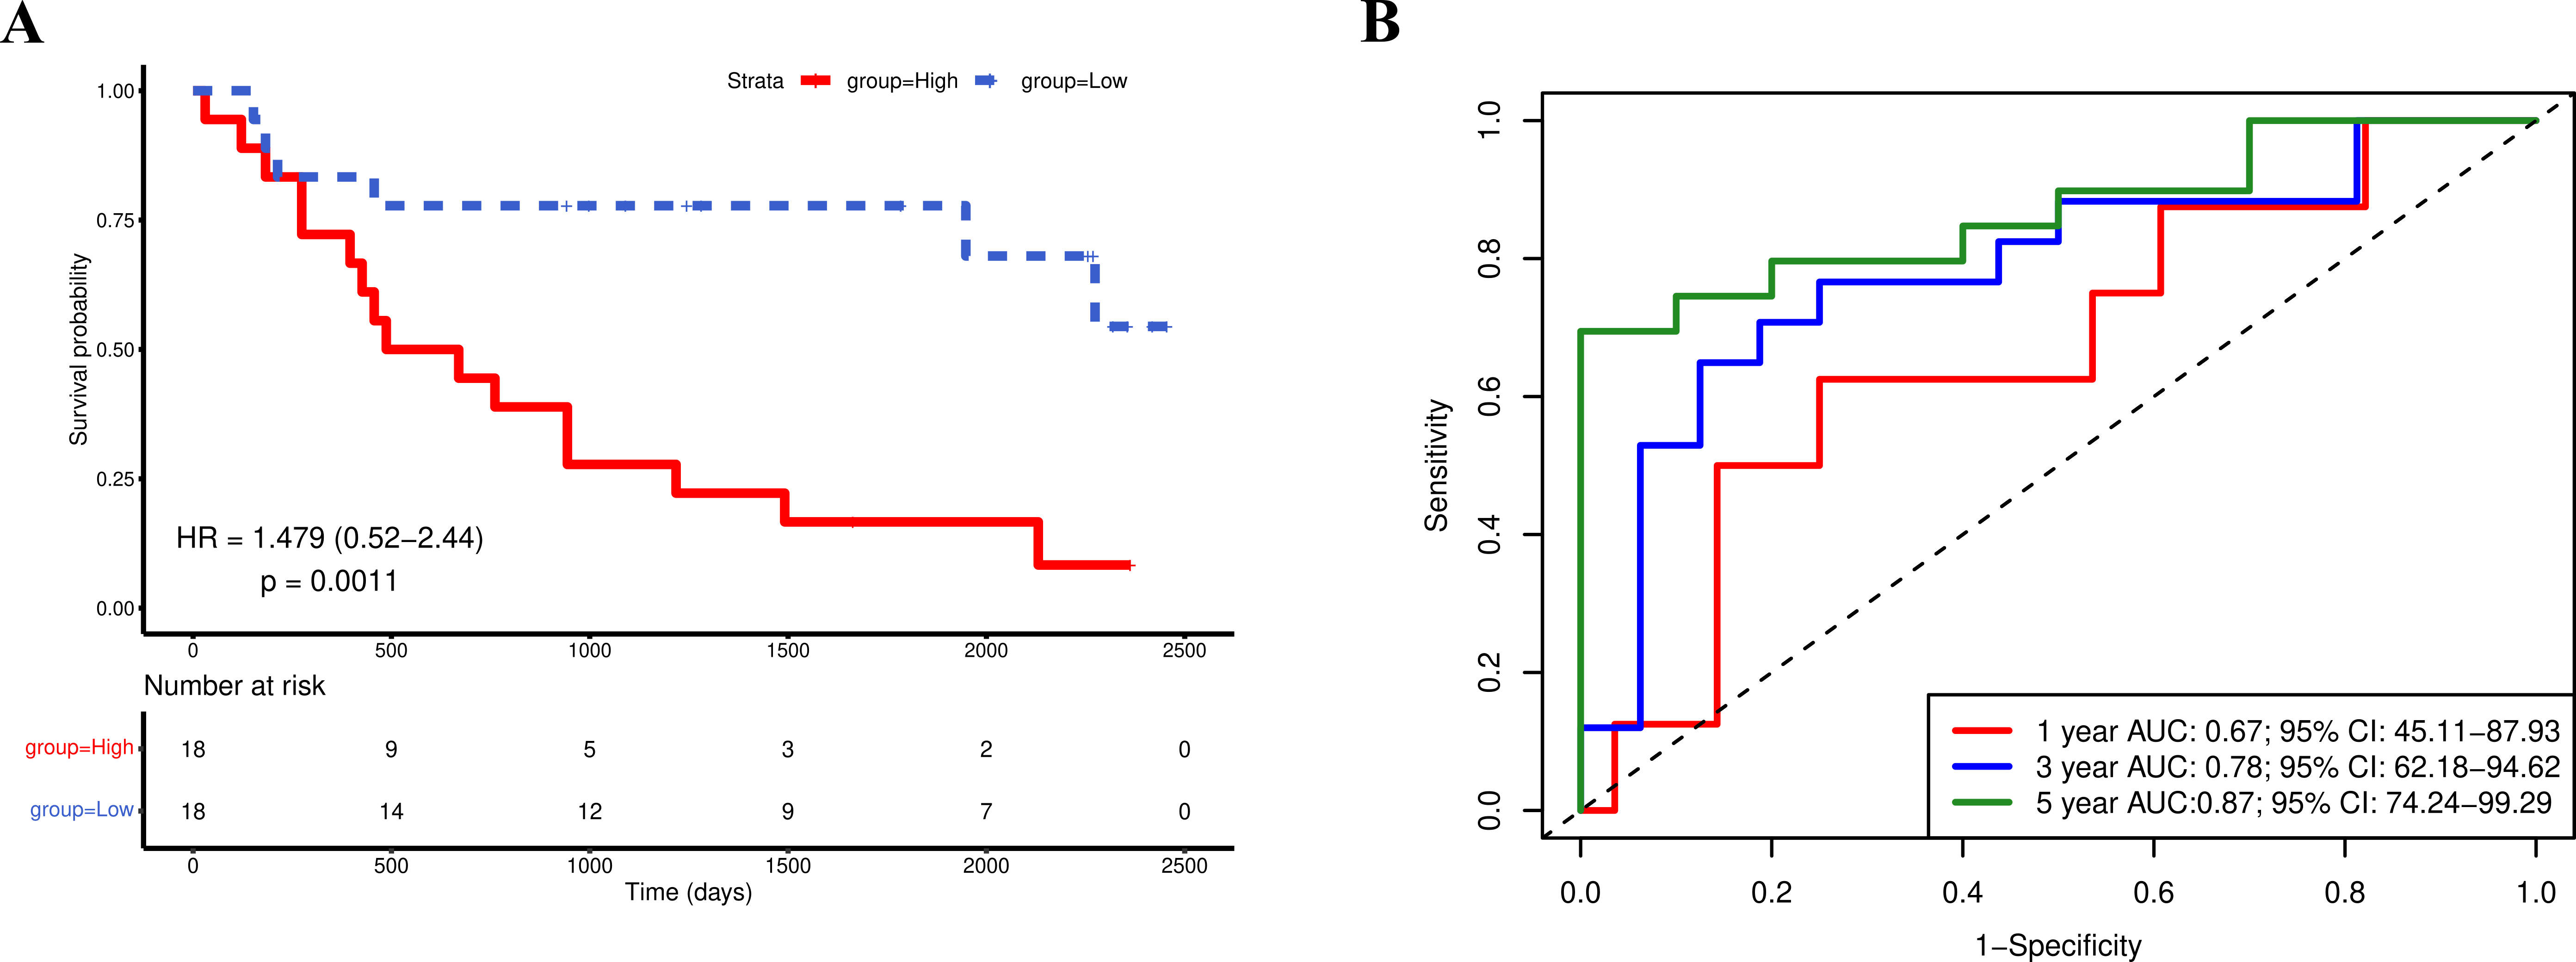
\includegraphics[width=1\textwidth]{Chapter3/Figures/Figure_3.png}
  \caption[Validation dataset plots]{(a) Kaplan-Meier plot in the validation dataset stratified by high-risk and low-risk groups as defined by the median prognostic index cutoff point, including log-rank P value. (b) ROC analysis and AUC prediction accuracy of the prognostic index in the validation dataset}
    \label{Figure3}
\end{figure}


\paragraph{Comparison to published signatures}
When comparing our model to published PCa gene signatures, we observed a lower Harrell’s C-index (0.71) in the external validation cohort compared to the highest-performing model by Long et al. (0.98) (Table \ref{table3}) \cite{Long2014}. The time-dependent AUCs of our model improved over longer follow-up periods, increasing from 0.67 at year 1, to 0.78 at year 2, and 0.87 at year 5. Notably, only two genes from our model - SFRP4 and BGN - were shared with existing published signatures, suggesting that our model captures a largely distinct set of genes associated with BCR. 
\par
The table of summary statistics generated when comparing our model to published signatures is available in Supplementary Table \ref{chp4supptable8}. 12 published signatures containing more than 28 predictors were removed from the summary statistics; \textit{NA} values for Harrell's C-index, substantial hazard ratios, large confidence intervals, and non-significant \textit{P} values were indicative of overfitting to the validation dataset, rendering comparisons infeasible.


\begin{table}[!t]
\begin{center}
\caption[Comparison to published signatures]{Signature size, Harrell's C-index and time-dependent AUC values for ceRNA network signature and published signatures in the validation dataset.\label{table3}}%
\footnotesize
\resizebox{\textwidth}{!}{
\begin{tabular*}{0.9\columnwidth}{@{\extracolsep\fill}lccccc@{\extracolsep\fill}}
  & & \textbf{Harrell's} & \multicolumn{3}{c}{\textbf{AUC (years)}} \\
  \cline{4-6}
    \textbf{Dataset} & \textbf{Genes} & \textbf{C-index} & \textbf{1} & \textbf{3} & \textbf{5} \\
    \midrule
    Agell \cite{Agell2012Nov} & 12 & 0.83 & 0.98  & 0.84  & 0.82  \\
    Bibikova \cite{Bibikova2007Jun} & 16 & 0.83 & 0.86  & 0.89  & 0.91  \\
    Bismar \cite{Cuzick2011Mar} & 12 & 0.76 &  0.83  & 0.78  & 0.81  \\
    \textbf{Digby et al.} & 23 & 0.71 & 0.67 & 0.78  & 0.87  \\
    Ding \cite{Ding2011Feb} & 4 & 0.64 & 0.55  & 0.69  & 0.80  \\
    Erho \cite{Erho2013Jun} & 19 & 0.89 & 0.99  & 0.91  & 0.95  \\
    Glinsky \cite{Glinsky2005Jun} & 11 & 0.82 & 0.81  & 0.84  & 0.81  \\
    Irshad \cite{Irshad2013Sep} & 19 & 0.89 & 0.92  & 0.96  & 0.96  \\
    Jia \cite{Jia2012} & 15 & 0.79 & 0.84  & 0.83  & 0.89  \\
    Klein \cite{Klein2014Sep} & 12 & 0.85 & 0.90  & 0.87  & 0.89  \\
    Long \cite{Long2014} & 24 & 0.98 & 0.99  & 1.00  & 1.00  \\
    Nakagawa \cite{Nakagawa2008} & 17 & 0.91 & 0.97  & 0.94  & 0.99  \\
    Olmos \cite{Olmos2012Nov} & 9 & 0.75 & 0.89  & 0.76  & 0.79  \\
    Ramaswamy \cite{Ramaswamy2003Jan} & 17 & 0.86 & 0.88  & 0.90  & 0.91  \\
    Ross \cite{Ross2011} & 6 & 0.75 & 0.86  & 0.77  & 0.81  \\
    Sharma \cite{Sharma2013Jan} & 16 & 0.78 & 0.77  & 0.83  & 0.86  \\
    Talantov \cite{Talantov2010Oct} & 3 & 0.61 & 0.52 & 0.64 & 0.61 \\
    Yu \cite{Yu2007Nov} & 14 & 0.81 & 0.86  & 0.81  & 0.88  \\
    \bottomrule
\end{tabular*}}
\end{center}
\end{table}


\subsection{Discussion}\label{sec12}
This study developed and evaluated a prognostic model to estimate the 5-year risk of BCR in PCa by identifying a common ceRNA network in PCa and enzalutamide-resistance, attempting to capture the inflection point at which BCR occurs both post-operatively and post-administration of second-generation anti-androgen drugs. ceRNA network modelling and subsequent feature selection yielded a 23-gene signature which, although sensitive to heterogeneity, obtained moderate predictive power in the external validation dataset when compared to previously published signatures. Furthermore, the 23-gene signature comprises a largely unique set of genes compared with previously published signatures, suggesting it captures distinct underlying gene expression patterns which may help elucidate the mechanistic progression of BCR.

\par

Several limitations of our work must be considered. Rich clinical metadata, including pathological T and N stages, clinical T and M stages, and age, were available only in the TCGA-PRAD cohort. In the datasets used for model development, PSA and Gleason score were the only clinical variables consistently recorded, limiting feature selection to these two predictors. Ideally, future studies should obtain complete clinical metadata for modelling, as these clinical variables are likely to influence the final set of predictors identified through feature selection.  

\par

Secondly, we were unable to generate models containing suitable predictor set sizes using alternative feature selection methods such as glmnet (LASSO, Elastic Net) and Random Forests for Survival, Regression, and Classification (RFSRC). Whilst a comparative analysis of feature selection methods would have been of interest, we ultimately selected CoxBoost, as its \textit{minstep} and \textit{maxstep} parameters allowed us to constrain the final set of predictors to an appropriate size. 

\par

Finally, our analyses revealed notable between-study heterogeneity, both at the overall model performance level and at the individual gene effect level. Internal-external cross-validation showed variability in calibration slopes and moderate heterogeneity ($I^2 = 43.3\%$) despite relatively stable discrimination performance. Complementary mixed-effects Cox modelling indicated that while most genes had stable effects across studies, a subset exhibited moderate to high variability in their prognostic associations, reflecting potential cohort-specific factors.

\par 

Attempts to directly model these study-level differences through full mixed-effects models including random slopes (e.g. $coxme(Surv(time, event) \sim gene_1 ... gene_n + (1|study))$ ) were not computationally feasible, as we encountered model convergence issues. This limitation highlights the challenge of adequately accounting for complex heterogeneity structures in high-dimensional genomic data.


\par
Regarding the genes included in our prognostic model, several support current literature, whilst others are less studied, providing novel candidates for future works. B4GALT1 is one of seven beta-1, 4-galactosyltransferase (B4GALT) genes, upregulated in bladder, lung and renal cell carcinomas \cite{Xie2016May, Xie2018May, DeVitis2019Nov}. In CRPC, B4GALT1 was found to be silenced by the androgenic enzyme AKR1C3, facilitating CRPC progression \cite{Wang2020Sep}. Our results show that B4GALT1 was downregulated in PCa and enzalutamide-resistance (-0.45 LogFC), suggesting this genes protective effect against BCR is mitigated (HR=0.94 95\% CI= 0.84-1.05). Biglycan (BGN) is secreted from extracellular matrix fibroblasts and facilitates the assembly of collagen fibrils and bone matrix \cite{Xing2015Mar}. Given that the prostate secretes numerous glycoproteins and proteoglycans \cite{Munkley2016Jun}, interest in BGN as a prognostic marker in PCa has been raised. A study demonstrated a significant association between BGN overexpression and BCR, yet when combined with clinical covariates in a multivariate model, BGN did not provide independent prognostic value \cite{Jacobsen2017Aug}. For this reason, BGN may only provide utility when combined with other markers, as utilised by the Onco\textit{type} DX prostate cancer assay \cite{Knezevic2013Oct}. Our results show overexpression (1.37 logFC) and an association with BCR (HR=1.12, 95\% CI 0.95-1.32), in agreement with Jacobsen et al. \cite{Jacobsen2017Aug}.

\par

Research by Linder et al. shows that circadian transcription factors are regulated temporally at a transcriptional level, and are dysregulated when exposed to enzalutamide in CRPC \cite{Linder2022Jun}. BHLHE40 is a circadian rhythm factor and circadian repressor; downregulation in PCa is associated with poor outcome \cite{HeidariHorestani2024Dec}. Our findings show similar downregulation (-1.95 logFC), and effect (HR=0.96, 95\% CI=0.85-1.08) in our dataset. Fatty acid 2-hydroxylase gene (FA2H) silencing accelerated gastric, colorectal and breast cancer \cite{Yao2019Mar, LiangSun2021Jan, Dai2019Oct}, increasing resistance to cisplatin and PM02734 in gastric cancer cells and human cancer cell lines, respectively \cite{Yao2019Mar, Herrero2008Dec}. Our results found FA2H to be upregulated (0.62 logFC) and protective against BCR (HR=0.95, 95\% CI=0.85-1.05), in agreement with the CMU5 prognostic signature trained and tested on the TCGA-PRAD dataset \cite{Wang2020May}. Mitogen-activated protein kinase 8 interacting protein 2 (MAPK8IP2) was found to be upregulated in multiple cancers, associated with BCR in PCa and upregulated in CRPC samples \cite{Zeng2022Nov, Cheng2020Jun}, consistent with our findings (2.35 logFC, HR=1.07 95\% CI=0.95-1.21). Neuronal PAS domain-containing protein 2 (NPAS2) is involved in anaerobic glycolysis in PCa cells; our findings support statements regarding its upregulation in PCa (0.79 logFC) \cite{Ma2023Dec}. 

\par

Upregulation of plasma membrane-associated sialidase (NEU3) has been shown to induce expression of EGR-1, AR and PSA in LNCaP cells with and without androgen, progressing PCa \cite{Kawamura2012Jan}. We found NEU3 upregulated (0.51 logFC) and associated with BCR (HR=1.05, 95\% CI=0.95-1.16). Programmed cell death protein 4 (PDCD4) is a tumour suppressor, downregulated in cancers; consistent with our findings (-0.79 logFC), capable of regulating prostate cancer cell proliferation, apoptosis, and castration resistance \cite{Zennami2019Feb}.  Phytanoyl-CoA dioxygenase domain containing 1 (PHYHD1) is downregulated in both recurrent vs. non-recurrent MCRPC and tumour vs. normal samples \cite{Li2018Feb, Su2021Sep}, similar to our findings (-0.53 logFC) in PCa and Enzalutamide-resistant samples. In a study by Khristi et al. investigating transcriptional perturbations induced by Esr2 knockdown and subsequent development of prostatic hyperplasia in \textit{R. norvegicus} \cite{Khristi2019Mar}, Family with sequence similarity 227 member B (FAM277B) was downregulated. Whilst FAM227B exhibited a protective effect against BCR (HR=0.95, 95\% 0.86, 1.06) in our datasets, its protective effect was mitigated through downregulation (-0.62 logFC). 

\par

Secreted frizzled-related protein 4 (SFRP4), a modulator of the cancer-associated Wnt pathway, is correlated with PCa aggressiveness and is an independent predictor of PCa aggressiveness in seven independent datasets \cite{Mortensen2015Nov, Horvath2004Jan, Azad2015May, Sandsmark2017Oct}. SFRP4 is included in multiple prognostic signatures \cite{Feng2022Jan, Yimamu2022Dec}, including the commercially available Onco\textit{type} DX test \cite{Knezevic2013Oct}. We found SFRP4 to be upregulated (1.40 logFC) and associated with BCR (HR=1.07, 95\% CI=0.94-1.23). Secreted protein, acidic, rich in cysteine (SPARC) expression is highly expressed in patients experiencing metastases after radical therapy and associated with higher Gleason scores \cite{HutchSPARC, Lopez-Moncada2019Nov}. Our results contradict these studies (-0.48 logFC), yet corroborate findings from several studies demonstrating SPARC expression is downregulated in PCa \cite{Chekhun2024Feb, Shin2013Aug}. Our results demonstrate Limb Expression 1 (LIX1) is downregulated (-2.48 logFC), mitigating its protective effects against BCR (HR=0.87, 95\% CI=0.77-0.98), consistent with recent work by Fan et al. \cite{Fan2025Feb}. 

\par

Whilst some genes in our prognostic signature remain understudied in PCa, their broader functions and associations with cancers warrant discussion. BTN3A1, a butyrophilin family membrane protein involved in T-cell activation and immune regulation, has been implicated as a tumour suppressor in breast and non–small cell lung cancer, where lower expression is associated with worse outcomes \cite{Liang2021Aug}. We report similar trends (-1.41 logFC, HR=0.95, 95\% CI=0.85-1.06) in PCa. RBM47, an RNA-binding protein, functions as a tumour suppressor by regulating splicing and stabilising antitumor transcripts in breast cancer \cite{Vanharanta2014Jun}. Similarly, in renal cell carcinoma, RBM47 acts as a tumour suppressor by inhibiting proliferation, migration, and invasion, with higher expression correlating with improved prognosis \cite{Wang2023Dec}. Our results show upregulation of RBM47 (0.36 logFC) with a protective effect against BCR (HR=0.92, 95\% CI=0.82-1.03). Rab11 family-interacting protein 2 (RAB11FIP2) overexpression is associated with tumour angiogenesis and poorer prognosis in colorectal cancer \cite{Dong2018Dec, Xu2016Feb}. Our results demonstrate downregulation in PCa with higher expression associated with a protective effect against BCR (-0.76 logFC, HR=0.91, 95\% CI=0.81-1.02). The mitochondrial transcription termination factor 4 (MTERF4) knockdown induces apoptosis, whilst overexpression promotes cell proliferation in HeLa cells \cite{Yu2011May}. We observed upregulation and a protective effect against BCR in our data (1.04 logFC, HR=0.94, 95\% CI=0.85-1.05).

\par 

Cyclic nucleotide binding domain containing 2 (CNBD2) is a prognostic marker in pancreatic cancer, where lower expression is associated with poor outcomes \cite{Uhlen2017Aug}. Our results demonstrate low levels of upregulation are associated with BCR (0.45 logFC, HR=1.06, 95\% CI=0.95-1.18). Overexpression of the ring finger protein 122 (RNF122) gene in glioblastoma samples and cell lines is associated with tumour progression via the  JAK2/STAT3/c‐Myc signaling pathway \cite{Xiao2024Sep}. We observed downregulation (-0.59 logFC), mitigating the protective effect of the gene (HR=0.94, 95\% CI 0.84, 1.06). SS18-like 2 protein (SS18L2) knockdown in triple-negative breast cancer cell lines induces G2/M arrest and apoptosis \cite{Yedier-Bayram2022Aug}. No current literature links SS18L2 to prostate cancer, thus our findings showing upregulation of SS18L2 in prostate cancer and enzalutamide-resistant cell lines (0.54 logFC) and higher expression associated with BCR (HR=1.06, CI 95\% 0.96, 1.18) warrant further investigation.
\par


For the remaining genes IAH1 and RNASEH2B, little is currently known about their role in cancers. Their inclusion in the prognostic signature underscores the hypothesis-generating value of our model; they represent promising candidates for functional follow-up studies, which could uncover novel roles in tumour progression, treatment response, or disease etiology.

\subsection{Conclusion}\label{sec13}
In summary, we integrated the transcriptomic profiles of prostate cancer patients and enzalutamide-resistant LNCaP cell lines at the circRNA, miRNA, and mRNA levels to construct a competing endogenous RNA network as a prognostic tool for biochemical recurrence. By leveraging regulatory information from the network, rather than relying on traditional machine learning dimension reduction techniques, we derived a biologically informed gene signature associated with recurrence. We further provide robust model evaluation techniques, offering a reproducible framework for future studies in prostate cancer prognosis.


\subsection*{Acknowledgements}

The authors thank Dr. Marvin Lim and Dr. Elaine Kenny for generating sequencing data on LNCaP cell lines.

\subsection*{Author contributions statement}

\textbf{B.D}: Conceptualization, Methodology, Software, Formal Analysis, Data Curation, Writing - Original Draft. \textbf{S.P.F}: Resources, Writing - Review \& Editing, Supervision. \textbf{P.\'{O}.B}: Conceptualization, Writing - Review \& Editing, Supervision, Funding Acquisition.


\subsection*{Competing interests}
The authors declare no competing interests.

\subsection*{Data Availability}
The following publicly available resources were used to obtain circRNA, miRNA and mRNA expression datasets: \href{https://portal.gdc.cancer.gov}{GDC Data Portal}, \href{https://www.ncbi.nlm.nih.gov/geo}{Gene Expression Omnibus}, \href{https://www.ebi.ac.uk/biostudies/arrayexpress}{ArrayExpress}, \href{http://bioinfo.jialab-ucr.org/PCaDB/}{PCaDB}. LNCaP sequencing data generated for this study are available at GSE312115 using the access token erupkycyvpkvvoj and Supplementary File \hyperlink{chp4suppfile1}{1}, respectively. All code used in the manuscript analysis is freely available on \href{https://github.com/BarryDigby/pca_network}{Github}.

\subsection*{Funding}
This research was funded by Science Foundation Ireland, grant number 18/CRT/6214.


\subsection{Supplementary Tables}

% Figures
\renewcommand{\thefigure}{\chapternum.S\arabic{figure}}
\setcounter{figure}{0}

% Tables
\renewcommand{\thetable}{\chapternum.S\arabic{table}}
\setcounter{table}{0}


\begin{table*}[ht!]
\caption[Prostate cancer datasets used for network construction]{Prostate cancer datasets used for differential expression testing and subsequent network construction.}
\label{chp4supptable1}
\footnotesize
\resizebox{\textwidth}{!}{
	\begin{tabular}{lcccr}
	\toprule 
	\textbf{Data type} & \shortstack{\textbf{Sample size}\\\textbf{(tumor/normal)}} & \textbf{Series} & \textbf{Platform} & \textbf{Reference} 
	\\
	\toprule 
	circRNA & 10/0 & \href{https://www.ncbi.nlm.nih.gov/geo/query/acc.cgi?acc=GSE113153}{GSE113153} & GPL21825 & \cite{Yang2019}
	\\
	miRNA & 100/28 & \href{https://www.ncbi.nlm.nih.gov/geo/query/acc.cgi?acc=GSE21036}{GSE21036} & GPL8227 & \cite{Taylor2010Jul}
	\\ 
	miRNA & 20/20 & \href{https://www.ncbi.nlm.nih.gov/geo/query/acc.cgi?acc=GSE23022}{GSE23022} & GPL8786 & \cite{Wach2012}
	\\
	miRNA & 21/21 & \href{https://www.ncbi.nlm.nih.gov/geo/query/acc.cgi?acc=GSE36803}{GSE36803} & GPL8786 & \cite{Lin2013} 
	\\ 
	miRNA & 50/10 & \href{https://www.ncbi.nlm.nih.gov/geo/query/acc.cgi?acc=GSE45604}{GSE45604} & GPL14613 & \cite{CasanovaSalas2014} 
    \\
	miRNA & 53/4 & \href{https://www.ncbi.nlm.nih.gov/geo/query/acc.cgi?acc=GSE46738}{GSE46738} & GPL8786 & \cite{Leite2015}  
	\\ 
	miRNA & 498/52 & \href{https://portal.gdc.cancer.gov/repository}{TCGA} & Illumina HiSeq & \cite{Grossman2016}
	\\
	mRNA & 498/52 &  \href{https://portal.gdc.cancer.gov/repository}{TCGA} & Illumina HiSeq & \cite{Grossman2016} 
	\\
	\toprule
	\end{tabular}}
\end{table*}



\begin{table*}[hbt!]
\caption[Enzalutamide datasets used for network construction]{Enzalutamide datasets used for differential expression testing and subsequent network construction. Clone 1 (high ENZ-resistance), Clone 9 (moderate ENZ-resistance).}
\label{chp4supptable2}
\footnotesize
\resizebox{\textwidth}{!}{
	\begin{tabular}{llllr}
	\toprule
	\textbf{Data type} & \shortstack{\textbf{Description of LNCaP samples}\\\textbf{(\textit{n} per subgroup)}} & \textbf{Series} & \textbf{Platform} & \textbf{Reference} 
	\\
	\toprule
	circRNA & Clone 1, Clone 9, Control (n=3) & \href{https://www.ncbi.nlm.nih.gov/geo/query/acc.cgi?acc=GSE118959}{GSE118959} & GPL21825 & \cite{Greene2019,Lim2021Dec}
	\\
	miRNA & Clone 1, Clone 9, Control (n=3) & \href{https://www.ncbi.nlm.nih.gov/geo/query/acc.cgi?acc=GSE312115}{GSE312115} & Illumina MiSeq & \textit{Digby et al.}
	\\
	mRNA & 21, 14, 7, 0 days ENZ treated (n=3) & \href{https://www.ncbi.nlm.nih.gov/geo/query/acc.cgi?acc=GSE143408}{GSE143408} & GPL25684 & \cite{Tousignant2020}
	\\
	mRNA & 6 months ENZ treated, control (n=4) & \href{https://www.ncbi.nlm.nih.gov/geo/query/acc.cgi?acc=GSE78201}{GSE78201} & GPL10558 & \cite{Kregel2016}
	\\
	mRNA & ENZ treated, ENZ sensitive (n=4) & \href{https://www.ncbi.nlm.nih.gov/geo/query/acc.cgi?acc=GSE88752}{GSE88752} & GPL11154 & \cite{Li2018}
	\\
	mRNA & Clone 1, Clone 9, Control (n=3) & \textit{in-house} & Illumina NovaSeq & \textit{N/A}
	\\
	\toprule
	\end{tabular}}
\end{table*}




\begin{table*}[hbt!]
\caption[Summary of datasets used for prognostic signature development and validation]{Datasets used for prognostic model development and external validation (GSE46602). Sample sizes are reported as (BCR events/total) following removal of patients with missing BCR information.}
\label{chp4supptable3}
\footnotesize
\resizebox{\textwidth}{!}{
	\begin{tabular}{llllr}
	\toprule
	\textbf{Dataset} & \textbf{BCR events/total} & \textbf{Series} & \textbf{Platform} & \textbf{Reference}
	\\
	\toprule
	Belfast & 56/248 & \href{https://www.ncbi.nlm.nih.gov/geo/query/acc.cgi?acc=GSE116918}{GSE116918} & GPL25318 &  \cite{Jain2018}
	\\
        CIT & 13/77 & \href{https://www.ncbi.nlm.nih.gov/geo/query/acc.cgi?acc=GSE54460}{GSE54460} & GPL11154 & \cite{Long2014}
        \\
        CMap & 58/200 & \href{https://www.ncbi.nlm.nih.gov/geo/query/acc.cgi?acc=GSE94767}{GSE94767} & GPL5175 & \cite{Luca2018}
        \\
        CPC & 36/99 & \href{https://www.ncbi.nlm.nih.gov/geo/query/acc.cgi?acc=GSE107299}{GSE107299} & GPL16686 & \cite{Sinha2019Mar}
        \\
        DKFZ & 24/105  & \href{https://ega-archive.org/studies/EGAS00001002923}{EGAS00001002923} & GPL11154 & \cite{Gerhauser2018}
        \\
        GSE46602 & 14/36 & \href{https://www.ncbi.nlm.nih.gov/geo/query/acc.cgi?acc=GSE46602}{GSE46602} & GPL570 & \cite{Mortensen2015Nov}
        \\
        GSE54460 & 40/91 & \href{https://www.ncbi.nlm.nih.gov/geo/query/acc.cgi?acc=GSE54460}{GSE54460} & GPL11154 & \cite{Long2014}
        \\
        Stockholm & 45/92 & \href{https://www.ncbi.nlm.nih.gov/geo/query/acc.cgi?acc=GSE70769}{GSE70769} & GPL10558 & \cite{RossAdams2015}
        \\
        TCGA & 99/463 & \href{https://portal.gdc.cancer.gov/repository}{TCGA} & Illumina HiSeq & \cite{Grossman2016}
        \\
        Taylor & 27/131 & \href{https://www.ncbi.nlm.nih.gov/geo/query/acc.cgi?acc=GSE21034}{GSE21034} & GPL5188 & \cite{Taylor2010Jul}
        \\
    \toprule
	\end{tabular}}
\end{table*}


\begin{table*}[h!]
  \centering
  \caption[Prognostic signatures used for comparison in the external validation dataset]{PCa prognostic signatures used for comparison in the external validation dataset}
  \label{chp4supptable4}
  \footnotesize
  \begin{adjustbox}{max width=\textwidth}
  \begin{tabular}{llr}
  \toprule 
  \textbf{Signature} & \textbf{Genes} & \textbf{Reference}
  \\
  \toprule 
  Agell & 12 &  \cite{Agell2012Nov}
  \\
  Bibikova & 16 & \cite{Bibikova2007Jun}
  \\ 
  Bismar & 12 & \cite{Bismar2006Jan}
  \\ 
  Cuzick & 31 & \cite{Cuzick2011Mar}
  \\
  Ding & 4 & \cite{Ding2011Feb}
  \\ 
  Erho & 19 & \cite{Erho2013Jun}
  \\ 
  Glinsky & 11 & \cite{Glinsky2005Jun}
  \\ 
  Irshad & 19 & \cite{Irshad2013Sep}
  \\
  Jia & 15 & \cite{Jia2012}
  \\
  Kamoun & 36 & \cite{Kamoun2018}
  \\ 
  Klein & 12 & \cite{Klein2014Sep}
  \\
  Li & 160 & \cite{Li2021May}
  \\
  Long & 24 & \cite{Long2014}
  \\
  Luca & 45 & \cite{Luca2018}
    \\
  Mo & 93 & \cite{Mo2018Apr}
    \\ 
  Nakagawa & 17 & \cite{Nakagawa2008} 
    \\
  Olmos & 9 & \cite{Olmos2012Nov} 
    \\
  Penney & 157 & \cite{Penney2011Jun} 
    \\
  Planche & 36 & \cite{Planche2011} 
    \\
Ramaswamy & 17 & \cite{Ramaswamy2003Jan} 
  \\
Ramos-Montoya & 222 & \cite{Ramos-Montoya2014May} 
  \\
Ross & 6 & \cite{Ross2011} 
  \\
Ross-Adams & 100 & \cite{Ross-Adams2015Jul} 
  \\
Sharma & 16 & \cite{Sharma2013Jan} 
  \\
Sinnott & 30 & \cite{Sinnott2017Jan} 
  \\
Talantov & 3 & \cite{Talantov2010Oct} 
  \\
Varambally & 44 & \cite{Varambally2005Nov}
  \\
Wu & 29 & \cite{Wu2013Apr} 
  \\
Yang & 28 & \cite{Yang2018May} 
  \\
Yu & 14 & \cite{Yu2007Nov} 
  \\
  \toprule
  \end{tabular}
  \end{adjustbox}
  \end{table*}


\clearpage

\begin{adjustwidth}{-0cm}{-0cm}
    \begin{longtblr}[
        entry = {Frequency of genes selected over 200 bootstrap samples},
        caption = {Frequency of genes selected by Coxboost over 200 bootstrap samples and passing Schoendfeld residuals filtering. Genes included in the final model are colored red.},
        label = {chp4supptable5}
        ]{
        colspec = {r X[4,l]},%% put weights for column width in []
        rowhead = 1
        }
        \hline
        \textbf{Frequency} & \textbf{Genes} \\
        \hline
        118 & gleason\_score \\
        105 & \textcolor{red}{RNASEH2C} \\
        102 & \textcolor{red}{SSTR1} \\
        94 & \textcolor{red}{SPARC} \\
        84 & \textcolor{red}{BGN} \\
        68 & \textcolor{red}{LIX1} \\
        60 & \textcolor{red}{NEU3} \\
        57 & \textcolor{red}{SFRP4} \\
        56 & \textcolor{red}{BHLHE40} \\
        54 & \textcolor{red}{SS18L2} \\
        52 & DCAF4L1 \\
        49 & \textcolor{red}{PHYHD1} \\
        48 & \textcolor{red}{PDCD4} \\
        46 & ST3GAL3 \\
        44 & TPCN2 \\
        43 & \textcolor{red}{CNBD2} \\
        42 & CELF5, SMCO3 \\
        41 & \textcolor{red}{FAM227B} \\
        39 & \textcolor{red}{RAB11FIP2} \\
        37 & POLR2L \\
        35 & LMO2, \textcolor{red}{NPAS2} \\
        34 & \textcolor{red}{BTN3A1}, DOCK6, PRDM1, ZNF287 \\
        33 & LRIF1, \textcolor{red}{RNF122} \\
        32 & HLX, \textcolor{red}{MTERF4} \\
        31 & REG4, SLC9B1, SRF \\
        30 & GLIPR2, \textcolor{red}{IAH1} \\
        29 & SLX4IP \\
        28 & COX6C, \textcolor{red}{FA2H}, NUS1 \\
        26 & RPIA \\
        25 & DLG3, MIEN1 \\
        24 & ACVRL1, \textcolor{red}{RBM47}, SLC35G1 \\
        23 & DDAH1, SLC2A4, SLC39A14, ZFPL1 \\
        22 & CDK17 \\
        21 & \textcolor{red}{MAPK8IP2}, SLCO5A1, ZNF623 \\
        20 & ZNF518B \\
        19 & HIC2, NDUFA1, TBC1D8, TMEM63C, TRAM2, TRIB1, UROS, ZNF268, ZNF804A \\
        18 & ATAD3C \\
        17 & CDCA7L, KIF21A, PRR13 \\
        16 & \textcolor{red}{B4GALT1}, BACE2, DHTKD1, RFXAP, TMEM151A \\
        15 & CDKN1A, DHX38, FOXL2, KCNC2 \\
        14 & AGRN, B3GAT1, TMC5 \\
        13 & CTHRC1, DPT, GSK3A, IGSF22, KCNS3, YKT6 \\
        12 & CHRM1, DHX40, GLP1R, MAEA, PAPSS1, PLIN1, ZBTB3 \\
        11 & FBXO43, OGFOD1, REPS1, RHOU, STARD3NL, TMSB10 \\
        10 & ALG9, C14orf39, C2orf68, CHRM3, CLPTM1, DUSP3, SARNP, TG, ZFR, ZNF138 \\
        9 & C1orf53, COX20, CRTC1, DNASE1L1, FAM117B, GCC1, GTF3C1, ITSN1, KAZN, LZIC, SH3RF1, SLC28A3, YPEL1, ZNF561 \\
        8 & ABCA12, ACAN, DECR1, DEDD, GPR37, LAMC1, MZB1, PACS1, POFUT2, TMEM54, TNS4 \\
        7 & ADGRG6, ATP1B3, BICD2, CRISPLD2, CSNK2A2, ELAVL2, EPSTI1, INHBB, KDM8, KL, LETMD1, MKRN1, MOCOS, MSR1, MUC6, NET1, RAB34, SCNN1G, SCRIB, WDR93 \\
        6 & CALML5, CBLB, ECHDC3, GBA2, HBQ1, HEY2, IGSF9B, KMO, MASP1, NSL1, RNF214, RPP30, SNAI2, STK35, TMEM164, TMEM44, TMF1, TRIM24, WASF2, ZNF664 \\
        5 & ABHD10, ANKFY1, ANXA3, CATSPERG, CDK10, COX10, FADS2, FBXO45, HS6ST1, JAG2, KREMEN1, OPA1, PABPC1L2A, PAPPA, PFKFB2, PGM2L1, PILRA, PPP4R4, SEC31B, SIAH3, SLC22A23, SLC22A3, STARD5, TEAD3, TMPRSS11F, USO1, WNT2B, ZNF830 \\
        4 & AKAP10, AQP4, C1orf216, CCDC120, CCNT2, CFAP44, EIF4G2, EPHA8, FADS1, GLUL, GRHL2, IPO11, KCNK9, LPIN1, LRTM2, MINK1, NAV3, NELFB, NFKBIL1, ORMDL1, PADI4, PPARGC1A, PPM1F, PPP3CB, SLC13A3, SLC25A21, SLC39A5, SP5, SUOX, TMEM192, TTC31 \\
        3 & ABHD13, ADAMTSL3, ANXA2, ARL8A, ARNT, ASCC3, ASPHD1, ATP6AP1, BRSK2, BTF3L4, CAMKV, CDCP1, CEP85L, CHST4, CLDN14, COL19A1, CPSF4, DSC3, ECHDC2, EFNA1, EHF, FAM43B, FMO5, FRMD5, GJB2, GMCL1, GNA14, GSAP, HBS1L, HCST, IL15RA, INSM2, IPO5, KIFC2, LRRC28, METAP1, MMP9, MNAT1, NAPA, NCALD, PHLDA3, PLAT, PWP1, RBL1, RIF1, SCAMP5, SGSM2, SIX4, SLC2A1, SNRPE, TCEANC2, THYN1, ZFP28, ZNF768 \\
        2 & ABRACL, ACSS2, ACTR3, AJAP1, ALX4, ASB4, BUD31, C3orf62, CACNA2D2, CACNB3, CENPQ, COL2A1, CTDSP2, DLGAP2, DRAM1, EBF2, EIF2B1, EYS, FMOD, GALNT10, GALNT11, HIC1, HMGCLL1, HNRNPA0, IBA57, IPO8, KIF20B, LGI3, LMTK2, LONRF1, LRRC61, LTA4H, MAK16, MCFD2, MCM3, MEIS1, MIOS, MIS12, MTERF2, NCDN, NDE1, NFIC, NFXL1, PER1, PLEKHM3, PPA2, RNMT, RPE65, RPS6KL1, SCFD1, SLC12A7, SLC5A9, SLCO3A1, SMG9, SRRD, SYNC, TH, THUMPD2, TOE1, TSC22D4, TTLL5, TTPA, TXLNB, UBE2E3, ULK1, UQCRB, USPL1, VDR, WDR59, WWTR1, YWHAG, ZDHHC18, ZMYM1, ZNF142, ZNF267, ZNF347, ZNF460, ZNF532, ZNF546 \\
        1 & ACVR2B, AKIRIN1, ANKRD53, ANXA5, ARSB, ASB1, BICC1, C19orf81, C2orf49, CAMLG, CATSPERB, CCND3, CEP120, CNIH4, CNP, COPB2, CUL5, CYP2E1, DAGLB, DDX3Y, DDX5, DENND4B, DFFA, DIRAS2, DYNC2LI1, EAF1, EDAR, EFHC1, EIF5, EMILIN2, ENOSF1, EPHA10, EPHB3, ESD, F10, FAM171A1, FBXO24, FRAT1, GIGYF1, GIT1, GPR87, GSR, HABP2, HEYL, HIF1A, HINFP, HPD, HSD11B1, IFI27L1, IFRD1, IFT81, IGDCC3, ING5, INPP5E, INPP5F, ISL1, ITGA5, KLK5, LEF1, LINGO1, LYRM7, MAG, MAOB, MARVELD2, MDH1B, ME1, MED6, MFSD10, MGAT5B, MORC2, MSANTD1, MTMR9, MUC4, NDUFA10, NKAIN1, NLRP9, NOL7, NRG4, NSRP1, NUMBL, NUP43, NXPH1, PBLD, PCDH1, PCDHB10, PCNP, PDIK1L, PHF19, PKHD1L1, PM20D2, PON2, PREB, PRMT9, PRPF39, PRRX1, QRFPR, QRSL1, RABIF, RALY, RASSF2, REN, RIT2, RNF168, RSRP1, SLC22A2, SLC25A37, SLC35F3, SLC36A4, SLC7A9, SRSF6, STKLD1, STRIP2, STX7, SYT7, TBCC, TMEM109, TMEM150C, TOR1B, TRIM59, TRPC4, TRUB1, UBA1, VPS54, ZC2HC1C, ZNF134, ZNF212, ZNF281, ZNF585B, ZNF706, ZNF791, ZNF862, ZRANB2 \\
        \hline
    \end{longtblr}
\end{adjustwidth}



\begin{table*}[t]
  \begin{adjustwidth}{-0.0in}{0in}
  \centering
  \caption[Model performance across internal-external cross-validation folds]{Prognostic model performance across internal-external cross-validation folds. Regular font study names represent the derivation dataset, whilst study names in bold represent the validation dataset. The derivation dataset represents a combination of all studies except the study listed, which is reserved as the validation dataset.}
  \label{chp4supptable6}
  \resizebox{1.05\linewidth}{!}{
  \begin{tabular}{llllllllll}
  \\
  & \multicolumn{3}{c}{\textbf{Calibration slope}} & \multicolumn{2}{c}{\textbf{Chi-squared}} & & \multicolumn{3}{c}{\textbf{High risk stratum}}
  \\ \cmidrule(lr){2-4}\cmidrule(lr){5-6}\cmidrule(lr){8-10}
  & \textbf{coef} & \textbf{(95\% CI)} & \textbf{P-value} & \textbf{\(\chi^2_5\)} & \textbf{P-value} & \textbf{Harrell's C} & \textbf{Hazard ratio} & \textbf{(95\% CI)} & \textbf{P-value}
  \\
  \toprule
  Belfast & 1.46 & (1.28, 1.65) & 6.14e-57 & 0 & 1 & 0.73 & 1.41 & (1.15, 1.66) & 7.13e-28 \\
  \textbf{Belfast} & 2.28 & (1.63, 2.93) & 7.61e-12 & 0 & 1 & 0.76 & 1.67 & (0.99, 2.35) & 1.70e-06 \\
  \toprule
  CIT & 1.61 & (1.42, 1.79) & 2.35e-66 & 0 & 1 & 0.73 & 1.38 & (1.14, 1.62) & 4.34e-30 \\
  \textbf{CIT} & 1.27 & (0.42, 2.11) & 3.30e-03 & 0 & 1 & 0.69 & 1.22 & (–0.07, 2.51) & 6.38e-02 \\
  \toprule
  CMap & 1.68 & (1.48, 1.88) & 1.76e-61 & 0 & 1 & 0.74 & 1.47 & (1.21, 1.73) & 1.31e-28 \\
  \textbf{CMap} & 1.19 & (0.77, 1.62) & 3.75e-08 & 0 & 1 & 0.68 & 1.00 & (0.44, 1.57) & 5.19e-04 \\
  \toprule
  CPC & 1.59 & (1.41, 1.78) & 4.63e-64 & 0 & 1 & 0.73 & 1.38 & (1.14, 1.63) & 3.40e-28 \\
  \textbf{CPC} & 1.48 & (0.81, 2.15) & 1.33e-05 & 0 & 1 & 0.71 & 1.23 & (0.50, 1.97) & 1.03e-03 \\
  \toprule
  DKFZ & 1.52 & (1.33, 1.70) & 2.16e-56 & 0 & 1 & 0.72 & 1.34 & (1.11, 1.58) & 3.06e-28 \\
  \textbf{DKFZ} & 1.83 & (1.25, 2.40) & 4.51e-10 & 0 & 1 & 0.84 & 2.28 & (1.07, 3.50) & 2.33e-04 \\
  \toprule
  GSE54460 & 1.60 & (1.41, 1.79) & 2.25e-63 & 0 & 1 & 0.73 & 1.41 & (1.16, 1.66) & 1.07e-28 \\
  \textbf{GSE54460} & 2.02 & (1.28, 2.77) & 1.06e-07 & 0 & 1 & 0.74 & 1.36 & (0.65, 2.08) & 2.00e-04 \\
  \toprule
  Stockholm & 1.60 & (1.41, 1.80) & 3.25e-61 & 0 & 1 & 0.73 & 1.37 & (1.12, 1.62) & 3.44e-27 \\
  \textbf{Stockholm} & 1.60 & (1.09, 2.12) & 1.05e-09 & 0 & 1 & 0.74 & 1.56 & (0.88, 2.25) & 7.53e-06 \\
  \toprule
  TCGA & 1.68 & (1.48, 1.89) & 2.70e-57 & 0 & 1 & 0.74 & 1.47 & (1.19, 1.74) & 1.57e-25 \\
  \textbf{TCGA} & 1.29 & (0.95, 1.63) & 4.64e-14 & 0 & 1 & 0.71 & 1.25 & (0.79, 1.71) & 9.95e-08 \\
  \toprule
  Taylor & 1.56 & (1.38, 1.75) & 2.23e-62 & 0 & 1 & 0.72 & 1.40 & (1.15, 1.64) & 2.08e-29 \\
  \textbf{Taylor} & 1.98 & (1.25, 2.71) & 1.17e-07 & 0 & 1 & 0.80 & 1.89 & (0.83, 2.96) & 4.73e-04 \\

  \hline
  \end{tabular}
  }
  \end{adjustwidth}
\end{table*}




\begin{table*}[t]
  \begin{adjustwidth}{-0in}{0in}
  \centering
  \caption[Gene-level Cox mixed-effects model results with heterogeneity assessment]{Gene-level Cox mixed-effects model results with heterogeneity assessment. Heterogeneity labels refer to variance levels 0.0-0.05 "Low", 0.05-0.09 "Moderate" and $>$0.1 "High". R. slope var: Random slope variance, the degree of heterogeneity in each gene coefficient across studies.}
  \label{chp4supptable7}
  \resizebox{\linewidth}{!}{
  \begin{tabular}{lrrrrrrrr}
  \toprule
  \textbf{Gene} & \textbf{Coef} & \textbf{HR} & \textbf{95\% CI} & \textbf{SE} & \textbf{P-value} & \textbf{R. slope var} & \textbf{Heterogeneity} \\
  \midrule
  NEU3       & 0.161  & 1.175 & (1.068, 1.292) & 0.048 & 0.0009   & 0.0000  & Low \\
  PDCD4      & -0.307 & 0.735 & (0.665, 0.812) & 0.051 & 0.0000   & 0.0000  & Low \\
  RAB11FIP2  & -0.312 & 0.731 & (0.664, 0.804) & 0.049 & 0.0000   & 0.0000  & Low \\
  RNASEH2C   & 0.233  & 1.262 & (1.145, 1.392) & 0.050 & 0.0000   & 0.0001  & Low \\
  CNBD2      & 0.179  & 1.196 & (1.087, 1.317) & 0.049 & 0.0003   & 0.0001  & Low \\
  SS18L2     & 0.212  & 1.236 & (1.121, 1.364) & 0.050 & 0.0000   & 0.0012  & Low \\
  B4GALT1    & -0.295 & 0.743 & (0.662, 0.835) & 0.059 & 0.0000   & 0.0076  & Low \\
  RNF122     & -0.248 & 0.780 & (0.685, 0.888) & 0.066 & 0.0002   & 0.0109  & Low \\
  SFRP4      & 0.409  & 1.506 & (1.315, 1.723) & 0.069 & 0.0000   & 0.0148  & Low \\
  SSTR1      & 0.413  & 1.512 & (1.327, 1.723) & 0.067 & 0.0000   & 0.0179  & Low \\
  MAPK8IP2   & 0.308  & 1.361 & (1.176, 1.576) & 0.075 & 0.0000   & 0.0224  & Low \\
  BHLHE40    & -0.128 & 0.879 & (0.756, 1.022) & 0.077 & 0.0945   & 0.0257  & Low \\
  FAM227B    & -0.243 & 0.783 & (0.666, 0.921) & 0.082 & 0.0031   & 0.0314  & Low \\
  IAH1       & 0.204  & 1.226 & (1.037, 1.451) & 0.086 & 0.0170   & 0.0357  & Low \\
  BTN3A1     & -0.248 & 0.780 & (0.658, 0.923) & 0.086 & 0.0039   & 0.0376  & Low \\
  FA2H       & -0.262 & 0.768 & (0.644, 0.917) & 0.090 & 0.0036   & 0.0448  & Low \\
  RBM47      & -0.332 & 0.717 & (0.603, 0.853) & 0.089 & 0.0002   & 0.0470  & Low \\
  BGN        & 0.449  & 1.567 & (1.296, 1.893) & 0.097 & 0.0000   & 0.0494  & Low \\
  NPAS2      & -0.249 & 0.779 & (0.646, 0.938) & 0.095 & 0.0085   & 0.0502  & Moderate \\
  PHYHD1     & -0.400 & 0.670 & (0.524, 0.857) & 0.125 & 0.0015   & 0.1119  & High \\
  LIX1       & -0.584 & 0.557 & (0.428, 0.725) & 0.134 & 0.0000   & 0.1208  & High \\
  MTERF4     & -0.351 & 0.703 & (0.544, 0.909) & 0.131 & 0.0073   & 0.1298  & High \\
  SPARC      & 0.373  & 1.453 & (1.114, 1.895) & 0.135 & 0.0058   & 0.1340  & High \\
  \bottomrule
  \end{tabular}
  }
  \end{adjustwidth}
\end{table*}




\begin{table*}[t]
  \begin{adjustwidth}{-0in}{0in}
  \centering
  \caption[Comparison of ceRNA network derived model vs. published prognostic signatures]{Comparison of ceRNA network derived model vs. published prognostic signatures.}
  \label{chp4supptable8}
  \resizebox{1.05\linewidth}{!}{
  \begin{tabular}{lllllllllr}
  \\
  & \multicolumn{3}{c}{\textbf{Calibration slope}} & \multicolumn{2}{c}{\textbf{Chi-squared}} & & \multicolumn{3}{c}{\textbf{High risk stratum}}
  \\ \cmidrule(lr){2-4}\cmidrule(lr){5-6}\cmidrule(lr){8-10}
  & \textbf{coef} & \textbf{(95\% CI)} & \textbf{P-value} & \textbf{\(\chi^2_5\)} & \textbf{P-value} & \textbf{Harrell's C} & \textbf{Hazard ratio} & \textbf{(95\% CI)} & \textbf{P-value}
  \\
  \toprule
Agell & 1 & (0.59, 1.41) & 1.95e-06 & 0 & 1 & 0.83 & 1.71 & (0.71, 2.72) & 7.97e-04 \\
Bibikova & 1 & (0.59, 1.41) & 1.57e-06 & 0 & 1 & 0.83 & 1.98 & (0.96, 3.01) & 1.50e-04 \\
Bismar & 1 & (0.57, 1.43) & 5.93e-06 & 0 & 1 & 0.76 & 1.53 & (0.58, 2.49) & 1.65e-03 \\
\textbf{Digby} & 1.33 & (0.59, 2.06) & 3.81e-04 & 0 & 1 & 0.71 & 1.48 & (0.52, 2.44) & 2.57e-03 \\ 
Ding & 1 & (0.17, 1.83) & 0.0184 & 0 & 1 & 0.64 & 0.82 & (-0.05, 1.69) & 6.44e-02 \\
Erho & 1 & (0.62, 1.38) & 3.40e-07 & 0 & 1 & 0.89 & 2.67 & (1.41, 3.93) & 3.36e-05 \\
Glinsky & 1 & (0.58, 1.42) & 2.50e-06 & 0 & 1 & 0.82 & 1.77 & (0.77, 2.78) & 5.23e-04 \\
Irshad & 1 & (0.62, 1.38) & 3.46e-07 & 0 & 1 & 0.89 & 2.71 & (1.44, 3.97) & 2.67e-05 \\
Jia & 1 & (0.58, 1.42) & 2.71e-06 & 0 & 1 & 0.79 & 1.71 & (0.68, 2.75) & 1.13e-03 \\
Klein & 1 & (0.58, 1.42) & 2.82e-06 & 0 & 1 & 0.85 & 2.65 & (1.40, 3.89) & 3.14e-05 \\
Long & 0.98 & (0.46, 1.51) & 2.02e-04 & 0 & 1 & 0.98 & 3.13 & (1.62, 4.65) & 1.90e-04 \\ 
Nakagawa & 1 & (0.61, 1.39) & 6.39e-07 & 0 & 1 & 0.91 & 3.14 & (1.62, 4.65) & 4.77e-05 \\
Olmos & 1 & (0.51, 1.49) & 7.07e-05 & 0 & 1 & 0.75 & 1.24 & (0.36, 2.13) & 5.83e-03 \\
Ramaswamy & 1 & (0.59, 1.41) & 1.57e-06 & 0 & 1 & 0.86 & 2.15 & (1.03, 3.27) & 1.59e-04 \\
Ross & 1 & (0.49, 1.51) & 1.34e-04 & 0 & 1 & 0.75 & 1.26 & (0.35, 2.18) & 6.62e-03 \\
Sharma & 1 & (0.52, 1.48) & 4.54e-05 & 0 & 1 & 0.78 & 1.94 & (0.90, 2.98) & 2.56e-04 \\
Talantov & 1 & (-0.04, 2.04) & 5.97e-02 & 0 & 1 & 0.61 & 0.62 & (-0.24, 1.48) & 1.60e-01 \\
Yu & 1 & (0.60, 1.40) & 1.23e-06 & 0 & 1 & 0.81 & 2.05 & (0.92, 3.18) & 3.58e-04 \\
  \toprule
  \end{tabular}
  }
  \end{adjustwidth}
\end{table*}

\clearpage

\subsection{Supplementary Figures}

\begin{figure}[!h]
  \centering
  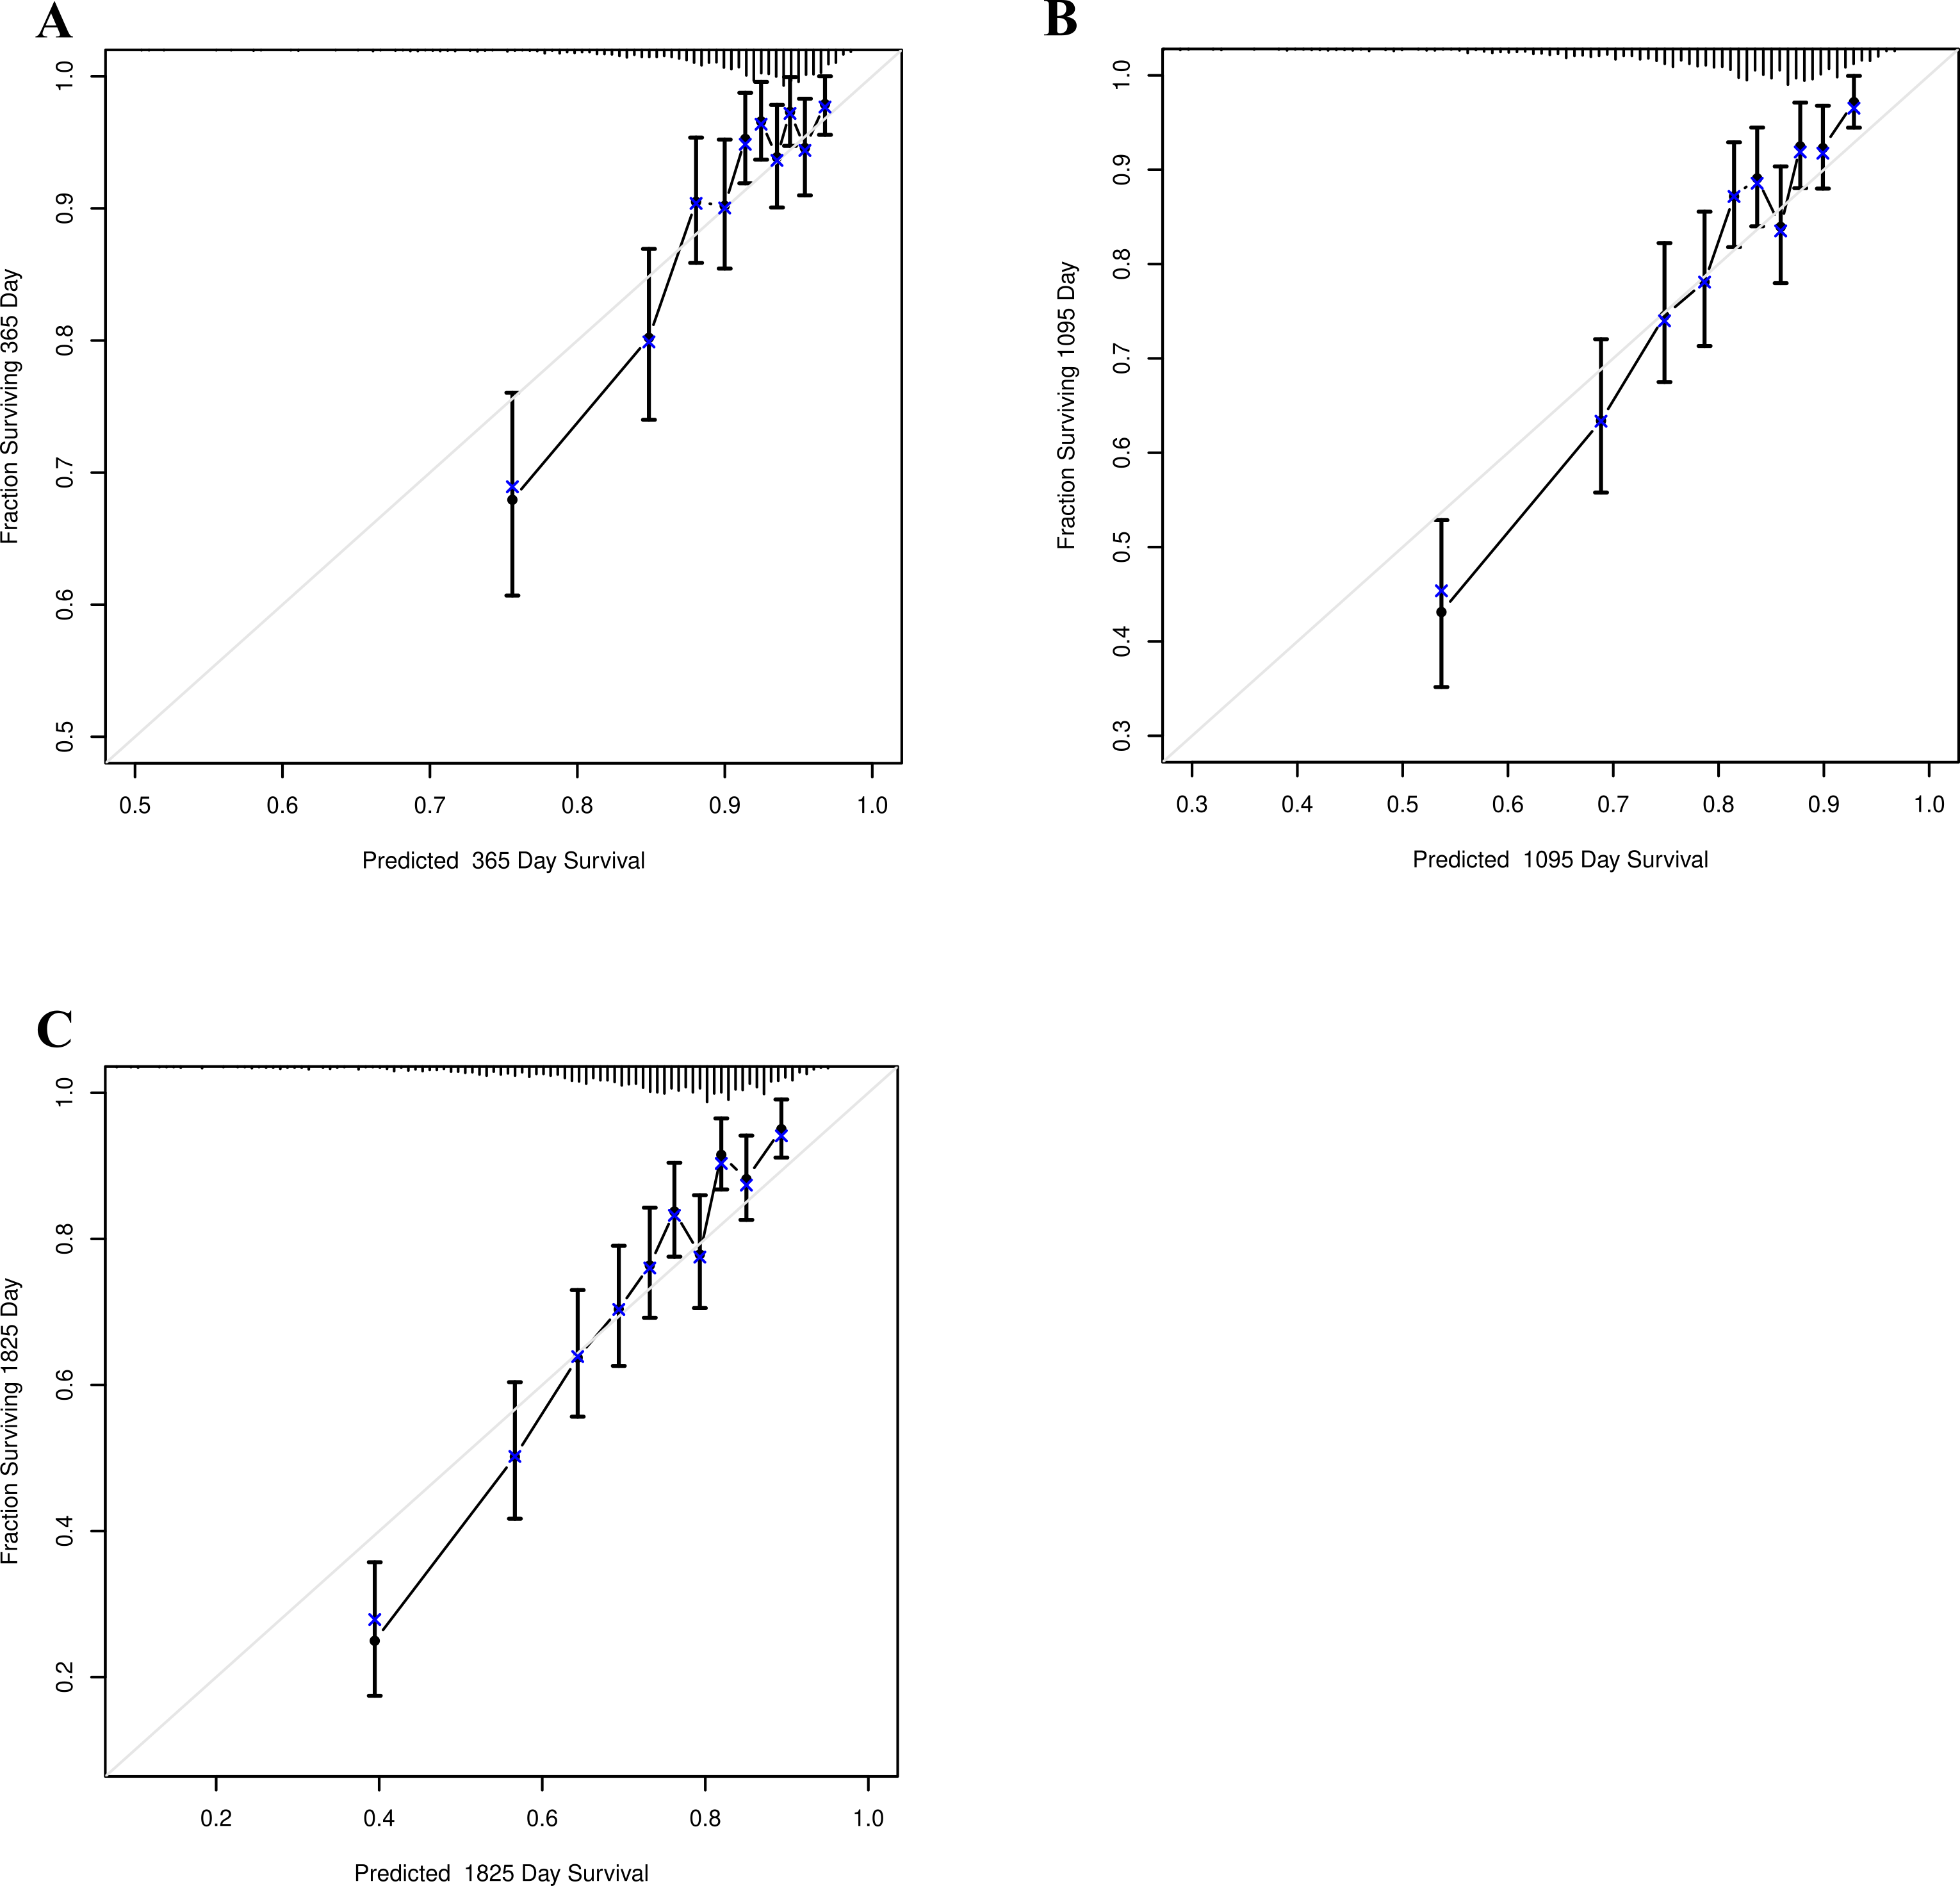
\includegraphics[width=\textwidth]{Chapter3/Figures/Supp_Figure1.png}
  \caption[Prognostic signature calibration curves]{Calibration curves plotting the estimated probabilities (x-axis) vs. the observed BCR events (y-axis) for years 1 (A), 3 (B) and 5 (C), respectively. Estimated probabilities were derived using the derivation dataset.}
  \label{chp4suppfigure1}
\end{figure}

\subsection{Supplementary Files}
\hypertarget{chp4suppfile1}{}

LNCaP miRNA sequencing counts are available online at the following \href{https://github.com/BarryDigby/pca_network/blob/main/mirna/LNCaP/mirna.tsv}{link}.
{\Huge \bfseries \noindent Chapter 6}
\vspace{-1em} 
\section*{\LARGE Discussion}
\addcontentsline{toc}{section}{6\quad Discussion}
\setcounter{section}{6}
\setcounter{subsection}{0}
\renewcommand{\chapternum}{6}

% Reset figure/table numbering per chapter
\renewcommand{\thefigure}{\chapternum.\arabic{figure}}
\setcounter{figure}{0}
\renewcommand{\thetable}{\chapternum.\arabic{table}}
\setcounter{table}{0}

\vspace{2em}

\subsection{Overview}
This thesis set out to address two interlinked obstacles that have constrained the study of circRNAs: the computational difficulty of detecting, quantifying, and reliably annotating circRNAs from high-throughput sequencing data, and the incomplete understanding of their post-transcriptional regulatory functions in oncogenesis and drug resistance. To this end, the work presented herein delivers two open-source software contributions to the bioinformatics and RNA biology communities alongside a translational investigation into the regulatory roles of circRNAs in PCa enzalutamide resistance and BCR, through the lens of the ceRNA network. circRNAs represent compelling candidates for both biomarker discovery and therapeutic intervention owing to their covalently closed loop structure, which lacks accessible 5' and 3' ends, conferring intrinsic resistance to exonucleolytic degradation and a markedly extended half-life relative to linear transcripts \cite{Salzman2012, Li2015Aug}.

In Chapter One, the biological foundation of androgen receptor signalling in prostate development, tissue homeostasis, and malignant transformation was described \cite{Rebello2021Feb}. While androgen-deprivation therapy and second-generation anti-androgens such as enzalutamide initially produce clinical responses, the selective pressure of AR blockade inevitably precipitates treatment failure, driving progression to castration-resistant prostate cancer and subsequent biochemical recurrence \cite{Scher2012Sep, Cornford2017, Rans2022, Shore2024}. The molecular mechanisms driving this progression—including AR gene amplification, point mutations within the ligand-binding domain, and the emergence of constitutively active splice variants such as \textit{AR-V7} \cite{Azad2015May, Hu2009Jan, Csizmarik2021Oct}—underscore the necessity for prognostic biomarkers capable of capturing latent therapeutic resistance.

Circular RNAs frequently harbour evolutionarily conserved microRNA response elements within their mature spliced sequences, enabling them to competitively bind and sequester miRNAs and relieve post-transcriptional repression on downstream messenger RNA targets within competing endogenous RNA networks \cite{Hansen2013Mar, Thomas2014Aug, Denzler2014Jun}. This regulatory interplay makes circRNAs attractive candidates for untangling complex oncogenic phenotypes such as therapeutic resistance. However, translating this mechanistic premise into reproducible prognostic models has historically been obstructed by bioinformatics bottlenecks: high discordance among back-splice junction detection algorithms, the absence of standardised quantification workflows, and fragmented public databases with conflicting coordinate systems \cite{Chen2023Jan, Digby2023Dec, Digby2024Dec}. This thesis systematically addresses these challenges across four research chapters. By first diagnosing tool-level discrepancies (Chapter Two), developing an automated consensus-based quantification pipeline in nf-core/circrna (Chapter Three), and creating a unified multi-database annotation resource in pycircdb (Chapter Four), these software contributions establish the scalable infrastructure needed to support complex circRNA analyses, complementing the translational investigation in Chapter Five where an enzalutamide-resistance ceRNA network was modelled to derive a 23-gene prognostic signature for biochemical recurrence in prostate cancer.

\subsection{Synopsis of Major Findings}
This thesis evaluated the computational landscape of circRNA detection, delivered two novel software frameworks that resolve challenges in circRNA quantification and annotation, and investigated the regulatory mechanism of non-coding RNAs in prostate cancer drug resistance. The principal findings of this work are:

\begin{itemize}
    \item \textbf{The computational landscape of circRNA detection is fragmented and lacks a gold standard.} A comprehensive evaluation of the computational strategies underpinning circRNA analysis - ranging from library enrichment protocols (such as ribonuclease R digestion and RPAD) to segmented-based and pseudo-reference mapping algorithms - revealed substantial discordance among established detection tools \cite{Panda2017Jul, Pandey2019Feb, Hansen2016Apr, Zeng2017Jun, Vromman2023Aug}. Benchmarking evidence demonstrated that individual tools exhibit high tool-specific false-positive rates and divergent sensitivities depending on aligner choices and filtering parameters. The findings strongly indicated that multi-tool consensus calling represents the most effective strategy to mitigate algorithmic blind spots, while identifying the absence of standardised coordinate conventions and nomenclature as a critical barrier to cross-study reproducibility \cite{CirComPara2, Chen2023Jan}.

    \item \textbf{nf-core/circrna delivers an automated, containerised, consensus-driven pipeline for end-to-end circRNA analysis.} To address the workflow fragmentation and tool discordance identified in Chapter Two, this work introduced nf-core/circrna, the first workflow to integrate circRNA quantification across seven tools, automated miRNA target prediction, and differential expression analysis into a single Nextflow DSL2 pipeline \cite{Digby2023Dec, DiTommaso2017, Ewels2020Mar}. Combinatorial evaluation of nf-core/circrna's seven quantification tools demonstrated that an ensemble of three tools requiring consensus support from at least two tools achieves an optimal trade-off between sensitivity ($97.2\%$), precision ($98.5\%$), and computational efficiency ($F_1 = 97.8\%$). Furthermore, benchmarking highlighted the robust individual performance of CIRIquant \cite{CIRIquant} and identified an elevated false-positive rate associated with DCC \cite{DCC} due to unconstrained STAR 2-pass chimeric mapping.

    \item \textbf{pycircdb unifies fragmented circRNA databases for high-throughput programmatic annotation.} To resolve the nomenclature and annotation bottlenecks identified throughout the literature \cite{Chen2023Jan}, this thesis delivered pycircdb, a Python-based command-line tool that harmonises nine public circRNA databases into a single queryable system \cite{Digby2024Dec}. pycircdb unifies genomic coordinates to a 0-based format, resolves hg19-hg38 liftovers while preserving segmental duplications, and uses Apache Hamilton with columnar Parquet storage. Consequently, it enables rapid batch annotation of candidate circRNAs with precomputed miRNA and RBP interactions on modest hardware (processing 300,000 circRNAs in 66.7s with 3.8 GB peak RAM and 4.2 GB disk footprint including database download).

    \item \textbf{A competing endogenous RNA network-derived signature predicts five-year biochemical recurrence in prostate cancer.} By integrating transcriptomic data from enzalutamide-resistant versus enzalutamide-sensitive LNCaP cell lines with clinical PCa patient cohorts across circRNA, miRNA, and mRNA biotypes, this work constructed a biologically constrained ceRNA network. This knowledge-based feature selection framework yielded a 23-gene prognostic signature predictive of five-year biochemical recurrence. The signature demonstrated robust discriminative performance across nine independent cohorts ($n=1{,}451$), achieving an apparent Harrell's C-index of 0.73, an optimism-corrected C-index of 0.68 via bootstrap resampling ($M=200$), and strong external validation ($C = 0.71$, five-year time-dependent $\text{AUC} = 0.87$) \cite{Mortensen2015Nov, Harrell1996Feb, Steyerberg2015Apr}. Crucially, the 23-gene signature was found to comprise a largely unique gene set relative to 30 published prognostic signatures, underscoring the discovery value of regulatory network modelling.
\end{itemize}

\subsection{Synthesis of Research Themes}

\subsubsection{Scalable, reproducible, and standardised workflows for circRNA analyses}
The computational challenges inherent in characterising circRNAs reflect a broader reproducibility crisis across high-throughput genomics and transcriptomics studies. Historically, computational pipelines frequently relied on bespoke, unversioned in-house scripts, non-containerised execution environments, and manual file formatting, leading to software decay and severe barriers to experimental replication \cite{Ziemann2023Oct}. In circRNA analyses, this fragmentation was compounded by the algorithmic divergence between segmented-anchor approaches (such as find\_circ and UROBORUS) and pseudo-reference methods (such as KNIFE and CIRIquant), where aligner-specific indexing heuristics, anchor-extension rules, and back-splice junction filtering thresholds produce widely divergent candidate sets across tools \cite{findcirc, UROBORUS, KNIFE, CIRIquant, Hansen2016Apr, Zeng2017Jun, Vromman2023Aug}. Furthermore, downstream public circRNA databases emerged as isolated web repositories with conflicting coordinate systems (0-based versus 1-based), asynchronous genome builds (hg19 and hg38), and idiosyncratic identifier schemes, hindering cross-database interoperability \cite{Chen2023Jan}.

In response to widespread reproducibility challenges in computational science, modern bioinformatics has undergone a transformative paradigm shift toward declarative, domain-specific workflow management systems, most notably Nextflow \cite{DiTommaso2017} and Snakemake \cite{Koster2012Oct, Molder2021Feb}. These systems decouple pipeline logic from compute infrastructure, allowing automated dependency resolution and scalable execution across local machines, high-performance compute clusters (such as SLURM, SGE or Kubernetes), and commercial cloud environments. In parallel, software containerisation through Docker, Apptainer (formerly Singularity), and community repositories such as BioContainers warehouse pinned versions of bioinformatics tools as container images \cite{Docker, Apptainer, daVeigaLeprevost2017Aug}, enabling reproducible analyses and alleviating dependency conflicts that have historically hindered analysis. These technical advances have been formalised through international standards and open-source initiatives, including the Global Alliance for Genomics and Health (GA4GH) Tool Registry and Workflow Execution Services \cite{Rehm2021Nov}, the Common Workflow Language (CWL) \cite{Crusoe2022Jun}, and centralised workflow registries such as WorkflowHub \cite{Goble2021Oct}, all driving adherence to the FAIR (Findable, Accessible, Interoperable, Reusable) data stewardship principles \cite{Wilkinson2016Mar}.

The computational contributions delivered in this thesis—\texttt{nf-core/circrna} (Chapter Three) and \texttt{pycircdb} (Chapter Four)—implement these modern workflow and data standardisation principles to establish an integrated analytical foundation for circRNA biology \cite{Digby2023Dec, Digby2024Dec}. Rather than proposing yet another detection algorithm, \texttt{nf-core/circrna} was engineered within the nf-core framework \cite{Ewels2020Mar}, embedding continuous integration testing, pinned containerised dependencies, and standardised configuration profiles across seven distinct circRNA quantification tools. By automating raw read quality control, multi-tool alignment, consensus-based back-splice junction filtering, mature spliced sequence extraction, miRNA response element prediction, and differential expression analysis into a single, platform-agnostic pipeline, \texttt{nf-core/circrna} mitigates the algorithmic blind spots and high false-positive rates inherent to single-tool analyses while ensuring deterministic execution across diverse computing platforms.

Complementing this upstream quantification pipeline, \texttt{pycircdb} resolves the persistent database fragmentation and annotation bottlenecks in the circRNA field. Moving away from relational database installations and static web interfaces that cannot scale to high-throughput batch queries, \texttt{pycircdb} restructures nine public repositories into a unified, 0-based coordinate framework. By leveraging columnar Apache Parquet storage hosted on public cloud infrastructure alongside Apache Hamilton directed acyclic graphs for parallel execution, \texttt{pycircdb} enables rapid, partition-aware batch queries of circRNA genomic annotations, spliced FASTA sequences, and precomputed miRNA and RBP interactions directly from the command line on standard workstation hardware. Together, \texttt{nf-core/circrna} and \texttt{pycircdb} advance computational reproducibility and lower technical barriers, bridging the gap between raw sequencing reads, circRNA quantification and standardised functional annotation.

\subsubsection{circRNAs as regulatory agents in the competing endogenous RNA network}
Complex human pathologies, particularly cancers, do not arise from isolated genetic abnormalities acting in a linear hierarchy; rather, they reflect systemic perturbations across interconnected networks \cite{Barabasi2011Jan, Ideker2012Jan}. Network biology posits that cellular phenotypes are governed by multi-layered regulatory graphs spanning protein-protein interactions, transcriptional circuits, and post-transcriptional cascades \cite{Califano2011Jan, Anastasiadou2018Jan}. Within this systems biology framework, the competing endogenous RNA (ceRNA) hypothesis formulated by Salmena et al. \cite{Salmena2011Aug} and expanded by Tay et al. \cite{Tay2014Aug} revealed a hidden post-transcriptional regulatory language: RNA transcripts harbouring shared microRNA response elements cross-regulate one another by competitively binding the limited intracellular pool of mature miRNAs. The subsequent discovery of circRNAs added an exceptionally stable, potent regulatory layer to this network architecture. Owing to their covalently closed loop structure, circRNAs resist exonucleolytic degradation by RNase R, conferring extended intracellular half-lives and enabling them to act as persistent molecular sponges that sequester miRNAs away from protein-coding mRNAs \cite{Salzman2012, Li2015Aug, Hansen2013Mar, Denzler2014Jun, Conn2024Sep}. This titrating activity coordinates critical oncogenic programmes, including cell proliferation, epithelial-to-mesenchymal transition, and acquired therapeutic resistance across diverse human malignancies \cite{Kristensen2019Nov, Hsiao2017, Lim2021Dec}.

In translational oncology, high-dimensional transcriptomic profiling regularly confronts the curse of dimensionality, where the number of measured genomic features vastly outweighs the number of available clinical patient samples. When using unconstrained data-driven feature selection or standard machine learning algorithms, models are acutely prone to overfitting technical noise, library batch effects, and platform-specific artefacts inherent to retrospective multicentre patient cohorts \cite{Riley2016Jun, Dhiman2021Oct, Steyerberg2015Apr}. In Chapter Five, this limitation was addressed by employing the topological constraints of the multi-layered ceRNA network as an explicit, knowledge-based inductive prior. Rather than selecting candidate prognostic biomarkers solely through unconstrained differential expression or univariate screening, candidate features were filtered to enforce coherent, reciprocal expression trajectories across circRNA, miRNA, and mRNA biotypes (upregulated circRNA $\rightarrow$ downregulated miRNA $\rightarrow$ upregulated mRNA, and vice versa).

Embedding this multi-omic regulatory network structure into the feature selection pipeline effectively regularised the high-dimensional search space prior to penalised survival modelling. As shown by the resulting 23-gene prognostic signature for prostate cancer biochemical recurrence, grounding biomarker discovery via a biologically constrained network topology insulated the model against cohort-specific batch variance. This inductive network resulted in a clinically transportable prognostic signal that generalised across diverse international patient cohorts evaluated under internal-external cross-validation, bootstrap resampling, and independent external validation \cite{Mortensen2015Nov, Harrell1996Feb, Steyerberg2015Apr}. Strikingly, the network-derived gene set demonstrated minimal overlap with thirty published prostate cancer prognostic panels, capturing a largely distinct transcriptional subspace \cite{Knezevic2013Oct, Cuzick2011Mar, Long2014Jun}. This highlights the discovery power of systems-level network modelling: by leveraging non-coding regulatory interactions as functional filters, researchers can uncover stable, clinically actionable biomarker programmes that conventional gene-centric and data-driven screening pipelines might overlook.

\subsubsection{Androgen receptor signalling plasticity, drug resistance and biomarker discovery}
Prostate cancer progression is fundamentally driven by the androgen receptor (AR) signalling axis. As detailed in Chapter One, canonical AR signalling governs prostate development, epithelial differentiation, and secretory function \cite{Rebello2021Feb}. Consequently, androgen-deprivation therapy (ADT) and surgical ablation have long served as the primary therapeutic action for localised and advanced disease. However, under the selective pressure of systemic androgen blockade, tumour cells undergo evolutionary adaptation, progressing to castration-resistant prostate cancer (CRPC) \cite{Scher2012Sep, Cornford2017}. Although second-generation anti-androgens such as enzalutamide competitively bind the AR ligand-binding domain to extend patient survival, intrinsic resistance occurs in up to 40\% of patients, and acquired resistance inevitably develops, heralding biochemical recurrence and metastatic dissemination \cite{Rans2022, Shore2024}.

The molecular underpinnings of enzalutamide resistance reflect transcriptional and genomic plasticity. Resistant tumour clones circumvent therapeutic inhibition through several distinct mechanisms, including AR gene amplification, point mutations within the ligand-binding domain (such as T877A, H874Y, and F876L, which mediate antagonist-to-agonist switching), and the generation of constitutively active splice variants lacking the ligand-binding domain, such as \textit{AR-V7} \cite{Azad2015May, Hu2009Jan, Csizmarik2021Oct}. Chapter Five leveraged in vitro cell-line models of acquired enzalutamide resistance (LNCaP clone models) to investigate transcriptomic alterations that accompany sustained anti-androgen exposure, capturing non-coding and coding RNA perturbations associated with treatment failure.

By integrating transcriptomic profiles from these cell-line models with PCa patient survival cohorts, Chapter Five assessed whether molecular programmes associated with acquired enzalutamide resistance could inform postoperative clinical risk stratification. Evaluating the 23-gene panel across retrospective cohorts demonstrated that transcriptional changes induced during acquired enzalutamide resistance are statistically informative for predicting time to biochemical recurrence following primary definitive therapy. Furthermore, several individual genes within the signature represent functionally relevant candidates in therapy resistance and tumour progression, including \textit{SFRP4}, \textit{B4GALT1}, \textit{FA2H}, and \textit{NEU3} \cite{Sandsmark2017Oct, DeVitis2019Nov, Yao2019Mar, Kawamura2012Jan}. While prospective clinical validation remains necessary, this work illustrates the feasibility of using in vitro drug-resistance signals, constrained by regulatory RNA networks, to guide the prioritisation of candidate prognostic biomarkers for postoperative disease monitoring.

\subsection{Methodological and Biological Limitations}

\subsubsection{Computational challenges in circRNA isoform resolution and cross-database mapping}
While the computational methodologies developed in this thesis advance circRNA detection and annotation, several limitations must be acknowledged:

\begin{itemize}
    \item \textbf{Short-read back-splice junction limitations}: Both nf-core/circrna and the primary databases integrated in pycircdb rely primarily on short-read Illumina sequencing data. Short reads span the back-splice junction (BSJ) but cannot resolve the internal exon composition or full-length mature sequence of circRNAs that contain multiple alternatively spliced internal exons or retained introns (EIcircRNAs) \cite{CIRI-full, isoCirc}. Consequently, predicted miRNA response elements derived from reference-guided exon concatenation may overestimate target sites if specific internal exons are skipped in vivo.
    
    \item \textbf{Upstream database dependency and longevity}: pycircdb aggregates nine curated resources, but the tool remains inherently dependent on the accuracy, curation quality, and ongoing availability of the underlying source files. Several circRNA databases originally surveyed in Chapter Two (e.g., CircRiC, Circ2Disease, Circ2Traits) have become unmaintained or inaccessible, reflecting a broader challenge of resource sustainability in bioinformatics. Furthermore, pycircdb is currently constrained to human genome builds (hg19 and hg38), limiting its utility for model organisms.

    \item \textbf{Coordinate liftover asymmetries}: Although pycircdb explicitly handles one-to-many mappings arising from segmental duplications and repetitive loci during UCSC liftOver between hg19 and hg38, a small fraction of circRNA coordinates situated in complex genomic regions fail cross-assembly liftover, resulting in build-specific records.
\end{itemize}

\subsubsection{Model limitations and cohort heterogeneity in prostate cancer prognosis}
The prognostic modelling framework established in Chapter Five provides valuable biological candidates, but exhibits important constraints:

\begin{itemize}
    \item \textbf{Clinical metadata constraints across historical cohorts}: In the meta-analysis of ten retrospective prostate cancer cohorts, comprehensive clinical metadata—such as pathological tumour stage, surgical margin status, and lymph node involvement—were inconsistently recorded across public repositories. Consequently, multivariate adjustments during feature selection and model evaluation were limited to serum PSA and Gleason score, the two parameters universally available across all derivation studies.
    
    \item \textbf{Between-study heterogeneity and calibration}: Internal-external cross-validation revealed moderate between-study heterogeneity in calibration slopes ($I^2 = 43.3\%$), driven by variations in microarray/sequencing platforms and patient demographic differences across international cohorts. Attempts to directly model between-study variation using multivariable mixed-effects models with random slopes proved computationally intractable due to convergence failure, reflecting the substantial sample sizes and BCR events required to reliably estimate high-dimensional random-effects covariance structures. 

    \item \textbf{In vitro modelling of drug resistance}: The ceRNA network was in part derived using enzalutamide-resistant LNCaP cell-line models in 2D monoculture. While these models effectively isolate cell-autonomous, AR-dependent resistance mechanisms, they cannot capture the complex stromal-epithelial interactions, immune infiltration, hypoxia, or lineage plasticity (such as neuroendocrine transdifferentiation) present in primary tumour microenvironments.

    \item \textbf{Requirement for functional wet-lab validation}: Although the 23-gene signature identified robust candidates with strong statistical support, the precise causal mechanisms by which these genes modulate biochemical recurrence and anti-androgen resistance require empirical validation through targeted CRISPR-Cas knockout, overexpression, and circRNA sponge rescue experiments.
\end{itemize}

\subsection{Future Perspectives}

\subsubsection{Next-generation long-read and spatial circRNA profiling}
The rapid evolution of sequencing technologies presents exciting avenues for expanding the computational tools developed in this thesis:

\begin{itemize}
    \item \textbf{Long-read full-length circRNA workflows}: Third-generation long-read sequencing technologies, including Oxford Nanopore Technologies (ONT) and Pacific Biosciences (PacBio), enable end-to-end sequencing of intact circular transcripts following rolling-circle amplification (RCA) or reverse transcription (RCRT) \cite{isoCirc, CIRIlong, circFLseq}. Future development of the nf-core ecosystem should incorporate a dedicated long-read circRNA workflow to reconstruct complete circular transcriptomes, resolving internal alternative splicing events and microRNA binding site architecture without reference-guided imputation.
    
    \item \textbf{Expansion of pycircdb across model organisms and single-cell modalities}: Future iterations of pycircdb will extend coordinate reconciliation and lookup capabilities to major model organisms (including \textit{Mus musculus}, \textit{Rattus norvegicus}, and \textit{Drosophila melanogaster}), matching the multi-species capacity of nf-core/circrna. Additionally, incorporating emerging single-cell and spatial transcriptomic circRNA data will allow researchers to query cell-type-specific and spatially resolved circRNA expression across complex tissues.

    \item \textbf{Integration with deep learning splicing predictors}: Integrating deep-learning models of non-canonical splicing and RNA secondary structure (e.g., JEDI, CIRI-deep) into nf-core/circrna will improve de novo back-splice junction classification, particularly in low-coverage or poly(A)-selected libraries \cite{JEDI, CIRIdeep}.
\end{itemize}

\subsubsection{Clinical translation, liquid biopsies and functional characterisation}
From a translational perspective, the findings presented in this thesis open several promising directions for clinical oncology:

\begin{itemize}
    \item \textbf{Prospective validation of the 23-gene prognostic signature}: The 23-gene signature derived in Chapter Five warrants further evaluation across emerging, contemporary clinical study datasets. Assessing its prognostic utility in cohorts treated with next-generation AR signalling inhibitors (such as enzalutamide, apalutamide, or darolutamide) will determine whether these candidate biomarkers retain discriminatory power in modern therapeutic regimens following radical prostatectomy.
    
    \item \textbf{Exosomal circRNA liquid biopsy assays}: Given the marked stability of circRNAs in extracellular vesicles and bodily fluids \cite{Li2015Aug, Memczak2015}, profiling the circRNAs identified within our enzalutamide-resistance ceRNA network in patient plasma or urinary exosomes represents a minimally invasive strategy for longitudinal disease monitoring and early detection of biochemical relapse.

    \item \textbf{Therapeutic targeting of oncogenic circRNA-miRNA axes}: Unravelling specific circRNA hubs that sponge tumour-suppressive miRNAs in enzalutamide-resistant cells provides actionable targets for therapeutic intervention. Synthetic circRNA sponges or antisense oligonucleotides (ASOs) engineered to disrupt specific back-splice junctions could potentially re-sensitise resistant tumour cells to androgen receptor antagonism.
\end{itemize}

\subsection{Concluding Remarks}
This thesis embarked on a dual investigation into circular RNAs, guided by the central premise that purpose-built computational methods are essential to deconstruct non-coding RNA networks and uncover clinically relevant insights. The body of work presented herein has advanced this premise through a series of interconnected contributions that span from algorithmic benchmarking and software engineering to translational biomarker discovery in prostate cancer.

By deconstructing the post-transcriptional regulatory architecture of anti-androgen resistance, this thesis has demonstrated that circular RNAs are active participants within the competing endogenous RNA network. It has shown that transcriptional perturbations accompanying acquired enzalutamide resistance can be captured through coherent circRNA-miRNA-mRNA network axes, identifying regulatory interactions that are statistically informative for predicting biochemical recurrence across multi-cohort clinical datasets.

Crucially, this work has moved beyond descriptive characterisation to deliver actionable computational frameworks. The development of nf-core/circrna and pycircdb provides the scientific community with reproducible, containerised infrastructure that resolves long-standing obstacles in consensus quantification, pipeline portability, and cross-database annotation \cite{Digby2023Dec, Digby2024Dec}. Furthermore, the establishment of a 23-gene prognostic signature illustrates the utility of using regulatory RNA networks to constrain feature selection, providing a robust paradigm for biomarker prioritisation that captures a largely distinct prognostic space relative to existing clinical panels \cite{Mortensen2015Nov, Harrell1996Feb, Steyerberg2015Apr}.

In conclusion, this thesis underscores that circular RNAs are not artefactual splicing curiosities, but stable, functionally active regulators of gene expression with tangible relevance in oncology. The computational pipelines and network-modelling strategies delivered in this work establish a systematic framework for deciphering the role of non-coding RNAs. By demonstrating that non-coding regulatory interactions can be systematically modelled, harmonised across databases, and linked to patient outcomes in prostate cancer, this work provides a foundation for the continued integration of circular RNAs into precision medicine and translational oncology. 

\bibliography{bibliography}

%remember to either sync with Mendeley or Zotero or upload a .bib file exported from those cite using \cite{CitationTagXXXX} there will be a list it's ok
\end{document}